\documentclass[12pt,a4paper]{extreport}
\usepackage[utf8]{inputenc}
%\usepackage[T5]{fontenc}
\usepackage[utf8]{vietnam}
%\usepackage{times}
\usepackage{enumerate}
\usepackage{enumitem}
\usepackage{multicol}
\usepackage{listings}
\usepackage[a4paper, top=3.5cm,bottom=3cm,left=3.5cm,right=2cm]{geometry}
\usepackage{verbatim}
\usepackage{graphicx}
\usepackage{url}
\usepackage{fancyhdr}
\usepackage{fancybox,framed}
\linespread{1.3}
\usepackage{lastpage}
\usepackage{floatrow}
\usepackage{floatrow}
\usepackage{array}
\usepackage{longtable}

\pagenumbering{arabic}
%\pagestyle{fancy}
\newfloatcommand{capbtabbox}{table}[][\FBwidth]
\usepackage{caption}
%\captionsetup[figure]{font=normalsize}
\usepackage{blindtext}
\usepackage{titlesec}
\usepackage[nottoc]{tocbibind}
\usepackage{bookmark}
%\usepackage[backend=bibtex,style=numeric,defernumbers=true,sorting=none]{biblatex}
% \usepackage[backend=biber]{biblatex}
%\bibliographystyle{plain}
%\bibliography{References/references.bib}

% ******************************************************************************
%\setlength{\topmargin}{-0.5cm} % Lề trên
%\setlength{\oddsidemargin}{-0.5cm} % Lề trái
%\setlength{\evensidemargin}{-0.5cm} % Lề phải
\setlength{\textwidth}{15.5cm} % Chiều rộng văn bản
\setlength{\textheight}{24cm} % Chiều cao văn bản
\setlength{\footskip}{1cm} % Khoảng cách giữa nội dung và số trang

% For line spacing 1.5
%\usepackage{setspace}
%\renewcommand{\baselinestretch}{1.5}

% ******************************************************************************
\usepackage{hyperref}
% \usepackage{hyperref}

% Cấu hình cho \paragraph để nó xuống hàng sau tiêu đề
\titleformat{\paragraph}[block]
{\normalfont\normalsize\bfseries}{\theparagraph}{1em}{}

\titlespacing*{\paragraph}
{0pt}{3.25ex plus 1ex minus .2ex}{1.5ex plus .2ex}

\setcounter{secnumdepth}{4}
\setcounter{tocdepth}{4}

\usepackage{array} % Gói cần thiết cho kiểu cột m{}

\titleformat*{\section}{\LARGE\bfseries}
\titleformat*{\subsection}{\Large\bfseries}
\titleformat*{\subsubsection}{\large\bfseries}


\usepackage{mdframed}

\usepackage{alltt}
\usepackage{color}
\usepackage{tocloft}

\usepackage{tikz}
\usetikzlibrary{calc}
\fancyfoot[C]{\thepage}

% Math
\usepackage{amsfonts}

\usepackage[numbers]{natbib}

%\newcommand{\tenSV}{Hoàng~Minh~Thanh} % Dấu ~ là khoảng trắng không được tách (các chữ nối với nhau bằng dấu ~ sẽ nằm cùng 1 dòng
%\newcommand{\mssv}{21C11029}
%\newcommand{\tenKL}{OPENHUMAN: HỆ THỐNG} % Chú ý dấu ~ trong tên khóa luận
%\newcommand{\tenGVHD}{PSG. TS. Lý Quốc Ngọc}
%\newcommand{\tenBM}{BM. Khoa~Học~Máy~Tính}
\author{Thanh Hoang-Minh \\ [2ex]
	Giảng viên hướng dẫn: \\ PGS. TS. Lý Quốc Ngọc}
%	\footnotesize \href{mailto:hmthanhgm@gmail.com}{(MSSV: 21C11029)}}

\institute{
	
\includegraphics[height=2cm]{hcmus.png}\\
	Faculty of Information Technology\\
	VNUHCM-University of Science}
\date{\today}

\usepackage{amsmath}
\usepackage{amssymb}
\usepackage{stmaryrd}

\usepackage[font=small,labelfont=bf]{subcaption}
\usepackage{listings}
\usepackage{color}

\usepackage{tocloft}
\usepackage{tabularx}
\usepackage{booktabs}
\usepackage{multirow}

\usepackage{tocloft}
\usepackage{tabularx}
\usepackage{booktabs}


% Chèn và định dạng mã giả
\usepackage{algorithm}
% \usepackage[ruled,vlined,linesnumbered]{algorithm2e}
\usepackage[noend]{algpseudocode}
\makeatletter
\def\BState{\State\hskip-\ALG@thistlm}
\makeatother


\usepackage{float}



\usepackage{cleveref}

% Redefine \tiny
\renewcommand{\tiny}{\fontsize{6.01}{7.21}\selectfont}    % MS Word 6pt ≈ LaTeX 6.01pt

% Redefine \scriptsize
\renewcommand{\scriptsize}{\fontsize{7.01}{8.41}\selectfont}  % MS Word 7pt ≈ LaTeX 7.01pt

% Redefine \footnotesize
\renewcommand{\footnotesize}{\fontsize{8.03}{9.63}\selectfont} % MS Word 8pt ≈ LaTeX 8.03pt

% Redefine \small
\renewcommand{\small}{\fontsize{12.03}{14.43}\selectfont}  % MS Word 12pt ≈ LaTeX 12.03pt

% Redefine \normalsize
\renewcommand{\normalsize}{\fontsize{13.04}{15.65}\selectfont} % MS Word 13pt ≈ LaTeX 13.04pt

% Redefine \large
\renewcommand{\large}{\fontsize{14.08}{16.90}\selectfont}  % MS Word 14pt ≈ LaTeX 14.08pt

% Redefine \Large
\renewcommand{\Large}{\fontsize{16.16}{19.26}\selectfont}  % MS Word 16pt ≈ LaTeX 16.16pt

% Redefine \LARGE
\renewcommand{\LARGE}{\fontsize{18.19}{21.83}\selectfont}  % MS Word 18pt ≈ LaTeX 18.19pt

% Redefine \huge
\renewcommand{\huge}{\fontsize{20.22}{24.26}\selectfont}   % MS Word 20pt ≈ LaTeX 20.22pt

% Redefine \Huge
\renewcommand{\Huge}{\fontsize{24.27}{29.12}\selectfont}   % MS Word 24pt ≈ LaTeX 24.27pt




% \titleformat{\section}[block]{\normalfont\Large\bfseries}{\thesection}{1em}{}

% \titleformat{\chapter}[display]
%   {\normalfont\LARGE\bfseries}   % Font size and weight for chapter title
%   {\thechapter}                  % Chapter number formatting
%   {1em}                          % Space between number and title
%   {}

% \makeatletter
% \def\@makechapterhead#1{
%   \vspace*{50pt}  % Vertical space before the chapter title
%   {\normalfont\Huge\bfseries\MakeUppercase{#1}}  % Font size and uppercase
%   \par\nobreak
%   \vskip 40pt
% }
% \makeatother


% \makeatletter
% \def\@makechapterhead#1{
%   \vspace*{50pt}  % Vertical space before the chapter title
%   {\normalfont\Huge\bfseries \MakeUppercase{Chương \thechapter: #1}}  % "Chapter" text and uppercase title
%   \par\nobreak
%   \vskip 40pt
% }
% \makeatother

%********************* Custom *********************

% \Huge
% Customize chapter title (equivalent to Word styles)
\titleformat{\chapter} % Adjust the chapter heading
  {\LARGE\bfseries}     % Font size: Huge (24.27pt), bold
  {\chaptername\ \MakeUppercase\thechapter.}       % Chapter number with a period
  {20pt}               % Space between the number and title
  {\MakeUppercase}     % Title format

% Customize section title (equivalent to Word styles)
\titleformat{\section} % Adjust the section heading
  {\Large\bfseries}    % Font size: LARGE (18.19pt), bold
  {\thesection}        % Section numbering
  {15pt}               % Space between the number and title
  {\LARGE\bfseries}    % Title format

% Customize subsection title
\titleformat{\subsection} % Adjust the subsection heading
  {\large\bfseries}      % Font size: Large (16.16pt), bold
  {\thesubsection}       % Subsection numbering
  {10pt}                 % Space between the number and title
  {\Large\bfseries}      % Title format

% Customize subsubsection title
\titleformat{\subsubsection} % Adjust the subsubsection heading
{\normalsize\bfseries}      % Font size: Large (16.16pt), bold
{\thesubsubsection}       % Subsection numbering
{10pt}                 % Space between the number and title
{\normalsize\bfseries}      % Title format

%********************* Custom *********************

\definecolor{customlinkcolor}{HTML}{0064E0}
\definecolor{customcitecolor}{HTML}{00AF19}
\definecolor{custompinkcolor}{HTML}{AF00E6}


\hypersetup{
	colorlinks=true,
	linkcolor=customlinkcolor,
	citecolor=customcitecolor,
	filecolor=magenta,
	urlcolor=custompinkcolor,
	citebordercolor=red,
	breaklinks=true,
	bookmarksopen=true,
	frenchlinks=true,
	linkbordercolor={0 0 1},
	menubordercolor={0 0 1},
	plainpages=false,
	urlbordercolor={0 0 1},
	pdftitle={OpenHuman: A conversational gesture synthesis system based on emotions and semantics},
	pdfauthor={Hoàng Minh Thanh},
	pdfpagemode=FullScreen,
	pdfborder={0 0 0}
}
% ~~~~~~~~~~~ Default ~~~~~~~~~~~
\newcommand{\ones}{\mathbf 1}
\newcommand{\reals}{{\mbox{\bf R}}}
\newcommand{\integers}{{\mbox{\bf Z}}}
\newcommand{\symm}{{\mbox{\bf S}}}  % symmetric matrices

\newcommand{\nullspace}{{\mathcal N}}
\newcommand{\range}{{\mathcal R}}
\newcommand{\Rank}{\mathop{\bf Rank}}
\newcommand{\Tr}{\mathop{\bf Tr}}
\newcommand{\diag}{\mathop{\bf diag}}
\newcommand{\card}{\mathop{\bf card}}
\newcommand{\rank}{\mathop{\bf rank}}
\newcommand{\conv}{\mathop{\bf conv}}
\newcommand{\prox}{\mathbf{prox}}

\newcommand{\Expect}{\mathop{\bf E{}}}
\newcommand{\Prob}{\mathop{\bf Prob}}
\newcommand{\Co}{{\mathop {\bf Co}}} % convex hull
\newcommand{\dist}{\mathop{\bf dist{}}}
\newcommand{\argmin}{\mathop{\rm argmin}}
\newcommand{\argmax}{\mathop{\rm argmax}}
\newcommand{\epi}{\mathop{\bf epi}} % epigraph
\newcommand{\Vol}{\mathop{\bf vol}}
\newcommand{\dom}{\mathop{\bf dom}} % domain
\newcommand{\intr}{\mathop{\bf int}}
\newcommand{\sign}{\mathop{\bf sign}}

\newcommand{\cf}{{\it cf.}}
\newcommand{\eg}{{\it e.g.}}
\newcommand{\ie}{{\it i.e.}}
\newcommand{\etc}{{\it etc.}}


% ~~~~~~~~~~~ Custom ~~~~~~~~~~~
%new commands
\newcommand{\der}[2]{\frac{d#1}{d#2}}
\newcommand{\nder}[3]{\frac{d^#1 #2}{d #3 ^ #1}}
\newcommand{\pder}[2]{\frac{\partial #1}{\partial #2}}
\newcommand{\npder}[3]{\frac{\partial ^#1 #2}{\partial #3^#1}}
\newcommand{\sentencelist}{def}
\newcommand{\overbar}[1]{\mkern 1.5mu\overline{\mkern-1.5mu#1\mkern-1.5mu}\mkern 1.5mu}
\newcommand{\lined}{\overbar}
\newcommand{\perm}[2]{{}^{#1}\!P_{#2}}
\newcommand{\comb}[2]{{}^{#1}C_{#2}}
\newcommand{\intall}{\int_{-\infty}^{\infty}}
\newcommand{\Var}[1]{\text{Var}\left(#1\right)}
\newcommand{\E}[1]{\text{E}\left(#1\right)}
\newcommand{\define}{\equiv}
\newcommand{\diff}[1]{\mathrm{d}#1}
\newcommand{\empy}[1]{{\color{darkorange}\emph{#1}}}
\newcommand{\empr}[1]{{\color{cardinalred}\emph{#1}}}

%********************* Custom ********************* 
\newcommand{\vardbtilde}[1]{\tilde{\raisebox{0pt}[0.85\height]{$\tilde{#1}$}}}
\newcommand{\defeq}{\coloneqq}
\newcommand{\grad}{\nabla}
%\newcommand{\E}{\mathbb{E}}
%\newcommand{\Var}{\mathrm{Var}}
\newcommand{\Cov}{\mathrm{Cov}}
\newcommand{\Ea}[1]{\E\left[#1\right]}
\newcommand{\Eb}[2]{\E_{#1}\!\left[#2\right]}
\newcommand{\Vara}[1]{\Var\left[#1\right]}
\newcommand{\Varb}[2]{\Var_{#1}\left[#2\right]}
\newcommand{\kl}[2]{D_{\mathrm{KL}}\!\left(#1 ~ \| ~ #2\right)}
\newcommand{\pdata}{{p_\mathrm{data}}}
\newcommand{\bA}{\mathbf{A}}
\newcommand{\bI}{\mathbf{I}}
\newcommand{\bJ}{\mathbf{J}}
\newcommand{\bH}{\mathbf{H}}
\newcommand{\bL}{\mathbf{L}}
\newcommand{\bM}{\mathbf{M}}
\newcommand{\bQ}{\mathbf{Q}}
\newcommand{\bR}{\mathbf{R}}
\newcommand{\bzero}{\mathbf{0}}
\newcommand{\bone}{\mathbf{1}}
\newcommand{\bb}{\mathbf{b}}
\newcommand{\bu}{\mathbf{u}}
\newcommand{\bv}{\mathbf{v}}
\newcommand{\bw}{\mathbf{w}}
\newcommand{\bx}{\mathbf{x}}
\newcommand{\by}{\mathbf{y}}
\newcommand{\bz}{\mathbf{z}}
\newcommand{\bxh}{\hat{\mathbf{x}}}
\newcommand{\btheta}{{\boldsymbol{\theta}}}
\newcommand{\bphi}{{\boldsymbol{\phi}}}
\newcommand{\bepsilon}{{\boldsymbol{\epsilon}}}
\newcommand{\bmu}{{\boldsymbol{\mu}}}
\newcommand{\bnu}{{\boldsymbol{\nu}}}
\newcommand{\bSigma}{{\boldsymbol{\Sigma}}}

\graphicspath{ {images/} }

\begin{document}

%\begin{titlepage}
	
	\begin{mdframed}[linewidth=1pt,
		linecolor=black,
		leftmargin=0,
		rightmargin=0,
		innertopmargin=20mm,
		innerbottommargin=20mm,
		innerleftmargin=10mm,
		innerrightmargin=10mm,
		skipabove=0,
		skipbelow=0]
		
		
		\centering
		\vspace*{1cm}
		
		{VIETNAM NATIONAL UNIVERSITY, HO CHI MINH CITY\par}
		\vspace{0.25cm}
		{\large \textbf{UNIVERSITY OF SCIENCE}\par}
		
		\vspace{2cm}
		
		{\large \MakeUppercase{\textbf{HOÀNG MINH THANH}}\par}
		
		\vspace{2cm}
		
		{\Large \bfseries
			\MakeUppercase{OpenHuman: A Conversational Gesture Synthesis System Based on Emotion and Semantics} \par}
		
		\vspace{3cm}
		
		{\large \bfseries
			MASTER'S THESIS\par}
		
		\vfill
		\vspace{3cm}
		
		{\small Ho Chi Minh City – 2024 \par}
	\end{mdframed}
\end{titlepage}

\pagenumbering{gobble}  
\pagebreak



\begin{titlepage}
	
	\begin{mdframed}[linewidth=1pt, 
		linecolor=black, 
		innerleftmargin=10mm, 
		innerrightmargin=10mm, 
		innertopmargin=10mm, 
		innerbottommargin=10mm]
		
		\centering
		\vspace*{1cm}
		
		{VIETNAM NATIONAL UNIVERSITY, HO CHI MINH CITY\par}
		\vspace{0.25cm}
		\textbf{UNIVERSITY OF SCIENCE}\\
		
		\vspace{2cm}
		
		\large HOÀNG MINH THANH \\
		
		\vspace{2cm}
		
		\Large \textbf{\MakeUppercase{OpenHuman: A Conversational Gesture Synthesis System Based on Emotion and Semantics}}\\
		
		\vspace{1cm}
		
		\flushleft
		{\normalsize Major: Computer Science}\\
		{\normalsize Program Code: 8480101}\\
		
		\vspace{2cm}
		
		\centering
		{\normalsize ACADEMIC SUPERVISOR}\\ 
		{\normalsize Assoc. Prof. Dr. LÝ QUỐC NGỌC}\\
		
		\vfill
		\vspace{3cm}
		
		{\small Ho Chi Minh City – 2024}
	\end{mdframed}
\end{titlepage}

\pagenumbering{gobble}  
\pagebreak
\pagenumbering{roman}

\pagebreak

%
%

\vspace{2cm}

\section*{\centering  \Large LỜI CAM ĐOAN}
\phantomsection
\addcontentsline{toc}{section}{Lời cam đoan}

\vspace{2cm}

{
Tôi cam đoan luận văn thạc sĩ ngành Khoa học máy tính, với đề tài OpenHuman: Hệ thống tổng hợp cử chỉ hội thoại dựa trên cảm xúc và ngữ nghĩa là công trình khoa học do tôi thực hiện dưới sự hướng dẫn của TS. Lý Quốc Ngọc.

Những kết quả nghiên cứu của luận văn hoàn toàn trung thực và chính xác. 

\begin{table}[H]
	\centering
	\begin{tabularx}{\textwidth}{X X}
		\textbf{\begin{tabular}[c]{@{}c@{}} \end{tabular}} &
		\textbf{\begin{tabular}[c]{@{}c@{}}
				\textit{TP. Hồ Chí Minh, ngày... tháng... năm...} \\
				HỌC VIÊN THỰC HIỆN \\
				\textit{(Ký và ghi rõ họ tên)}
		\end{tabular}}
	\end{tabularx}
\end{table}
\pagebreak

%
%\vspace{2cm}

\phantomsection
\addcontentsline{toc}{section}{Acknowledgements}

{\MakeUppercase\centering\Large\bfseries ACKNOWLEDGEMENTS}

\vspace{2cm}
{
	
	I would like to express my sincere gratitude to Mr. Lý Quốc Ngọc for his dedicated guidance, for sharing his knowledge and experience, and for offering valuable solutions throughout the process of completing this graduation thesis.
	
	My heartfelt thanks also go to the lecturers of the Faculty of Information Technology at the University of Science – Vietnam National University, Ho Chi Minh City, who have imparted invaluable knowledge to me during my studies.
	
	I would also like to thank the researchers whose work I have cited and built upon to complete this thesis.
	
	Finally, I am deeply grateful to my family, friends, and others who have always supported and encouraged me during the course of this thesis.
	
	Once again, my sincere thanks to all!
}

\pagebreak

%
%

% Ngắt việc thêm mục lục vào chính nó
\addtocontents{toc}{\protect\setcounter{tocdepth}{-1}}
% Căn giữa chữ "Mục lục"
% Bỏ qua tiêu đề tự động của \tableofcontents
\renewcommand{\contentsname}{}

%\renewcommand{\cftchappresnum}{\chaptername222 \quad \ \MakeUppercase} 
% Điều chỉnh cách hiển thị số chương trong TOC
\renewcommand{\cftchappresnum}{\chaptername\ \MakeUppercase} 
% Điều chỉnh khoảng cách giữa số chương và tiêu đề trong TOC
\setlength{\cftchapnumwidth}{6em} % Điều chỉnh độ rộng số chương
\setlength{\cftchapindent}{0em}     % Điều chỉnh độ thụt đầu dòng

\begin{center}
\textbf{\huge Table of Contents}
\end{center}

\tableofcontents
% Khôi phục lại thêm các mục vào mục lục sau đó
\addtocontents{toc}{\protect\setcounter{tocdepth}{2}}


\pagebreak

%
%
% Thêm "Danh mục hình ảnh" vào mục lục mà không liên quan đến \listoffigures
\phantomsection
% \addcontentsline{toc}{section}{Danh mục hình ảnh}

% Tạm thời ngừng việc thêm vào mục lục
\addtocontents{toc}{\protect\setcounter{tocdepth}{-1}}

% Sử dụng \listoffigures mà không hiển thị trên mục lục
\renewcommand{\listfigurename}{\makebox[\linewidth]{\Large DANH MỤC HÌNH ẢNH}}


\listoffigures

% Khôi phục lại việc thêm vào mục lục cho các phần sau
\addtocontents{toc}{\protect\setcounter{tocdepth}{2}}

\pagebreak


%% Manually add "List of Tables" to the table of contents without relying on \listoftables
\phantomsection
\addcontentsline{toc}{section}{List of Tables}

% Temporarily disable adding entries to the table of contents
\addtocontents{toc}{\protect\setcounter{tocdepth}{-1}}

% Use \listoftables without automatically adding it to the table of contents
\renewcommand{\listtablename}{\makebox[\linewidth]{\Large LIST OF TABLES}}

\listoftables

% Restore table of contents depth for subsequent sections
\addtocontents{toc}{\protect\setcounter{tocdepth}{2}}

%% Thêm "Danh mục các bảng số liệu" vào mục lục mà không liên quan đến \listoftables
\phantomsection
\addcontentsline{toc}{section}{Danh mục các thuật toán}


% Tạm thời ngừng việc thêm vào mục lục
\addtocontents{toc}{\protect\setcounter{tocdepth}{-1}}

% Sử dụng \listoftables mà không hiển thị trong mục lục
\renewcommand{\listalgorithmname}{\makebox[\linewidth]{\Large DANH MỤC CÁC THUẬT TOÁN}}

\listofalgorithms

% Khôi phục lại việc thêm vào mục lục cho các phần sau
\addtocontents{toc}{\protect\setcounter{tocdepth}{2}}

\pagebreak

%\pagebreak
\phantomsection
\addcontentsline{toc}{section}{List of Symbols and Abbreviations}
\section*{\textbf{ \Large LIST OF SYMBOLS AND ABBREVIATIONS}}

\begin{center}
\begin{tabular}{|p{3cm}|p{11cm}|}
\hline
\textbf{Symbol/Abbreviation} & \textbf{Full Description} \\
\hline
$\theta$ & Trainable weights to be learned \\
\hline
$\theta'$ & Learned weights used during sampling \\
\hline
$\epsilon$ & Noise added to the image \\
\hline
$\hat{\epsilon}$ & Predicted noise \\
\hline
$\epsilon_\theta$ or $f_\theta$ & Noise prediction function in DDPM with parameter $\theta$, where $f_\theta$ and $\epsilon_\theta$ are equivalent \\
\hline
$N$, $M$, $D$ & Numbers indicating the dimensions of matrices or vectors \\
\hline
$t: 1 \rightarrow T$ & Noise step $t$ from $t=1$ to $t=T$ \\
\hline
$n_{\operatorname{joins}}$ & Number of joints \\
\hline
$\mathcal{N}(a \bx, b^2)$ & The function $f(x) = a \bx + b \epsilon$ with $\epsilon \in \mathcal{N}(0, \mathbf{1})$ is equivalent to the normal distribution $\mathcal{N}(a \bx, b^2)$ \\
\hline
$\mathcal{N}(0, \mathbf{I})$ & Standard normal distribution with mean 0 and variance 1 \\
\hline
$\mathcal{N}(\bx_t; \mu_\theta, \Sigma_\theta)$ & Normal distribution where $\bx_t$ is the output, $\mu_\theta$ is the mean, and $\Sigma_\theta$ is the variance parameterized by $\theta$ \\
\hline
$\mathbf{x}_{t}^{1:M}$ & Gesture data at time step $t$, from frame 1 to frame $M$ \\
\hline
$\hat{\mathbf{x}}_0$ & Predicted data by the model \\
\hline
$f(x | y)$ & Conditional probability function: given $y$, find the probability of $x$ \\
\hline
$q(\bx_t | \bx_{t-1})$ & Conditional probability function in the forward diffusion process, given $\bx_{t-1}$, compute $\bx_t$ \\
\hline
$p_{\theta} (\bx_{t-1} | \bx_{t})$ & Conditional probability function in the denoising process: given $\bx_t$, compute $\bx_{t-1}$ with learnable parameter $\theta$ \\
\hline
$\boldsymbol{\mu}_\theta(\mathbf{x}_t, t)$ & Mean of $\bx_t$ at time step $t$ after passing through the model with parameter $\theta$ \\
\hline
$\mathbb{E}$ & Expectation \\
\hline
$\mathcal{L}^t$ & Loss function at time step $t$ \\
\hline
$G_\theta$ & The OHGesture model to be trained with parameter $\theta$ \\
\hline
$\prod^T_{t=1}$ & Product operator: $\prod_{t=1}^T a_t = a_1 \cdot a_2 \cdot \ldots \cdot a_T$ \\
\hline
\end{tabular}
\end{center}

\pagebreak

%\pagebreak
\phantomsection
\addcontentsline{toc}{section}{Glossary of Terms}
\section*{\textbf{ \Large GLOSSARY OF TERMS}}

\begin{center}
\begin{tabular}{|p{5cm}|p{10cm}|}
\hline
\textbf{Abbreviation} & \textbf{Full Meaning} \\
\hline
DDPM & Denoising Diffusion Probabilistic Models \\
\hline
OHGesture & Proposed model of the thesis \\
\hline
Sampling/Inference & The process of sampling or inference in the model \\
\hline
KL & Kullback–Leibler Divergence \\
\hline
MAE & Mean Absolute Error \\
\hline
MSE & Mean Squared Error \\
\hline
Forward Diffusion Process & A noise-adding process without weight-based training \\
\hline
\end{tabular}
\end{center}

\pagebreak

%%\phantomsection
\addcontentsline{toc}{section}{Trang thông tin luận văn tiếng Việt}
\begin{center}
{\centering \MakeUppercase \LARGE \fontsize{16.16}{19.26}\selectfont \bfseries TRANG THÔNG TIN LUẬN VĂN}
\end{center}
{
\setlength{\parindent}{0pt}
Tên đề tài luận văn: OpenHuman: Hệ thống tổng hợp cử chỉ hội thoại dựa trên cảm xúc và ngữ nghĩa \\
Ngành: Khoa học máy tính \\
Mã số ngành:  8480101 \\
Họ tên học viên cao học: Hoàng Minh Thanh \\
Khóa đào tạo: 31 \\
Người hướng dẫn khoa học: PGS. TS. Lý Quốc Ngọc \\
Cơ sở đào tạo: Trường Đại học Khoa học Tự nhiên, ĐHQG.HCM}

\vspace{10pt}
{\MakeUppercase \Large \bfseries 1. TÓM TẮT NỘI DUNG LUẬN VĂN:}
%\subsection*{1 TÓM TẮT NỘI DUNG LUẬN VĂN}

Cùng với sự bùng nổ của phần cứng, các mô hình ngôn ngữ lớn, sự bùng nổ của các hệ thống trí tuệ nhân tạo dựa trên văn bản như ChatGPT, CharacterAI, Gemini,..  và sự phát triển của đồ họa máy tính thì nút nghẽn cổ chai hiện nay để phát triển người kỹ thuật số (digital human) chính là khả năng tạo ra chuyển động của nhân vật tương ứng với văn bản hoặc giọng nói.
Một trong những khó khăn trong quá trình sinh cử chỉ là dữ liệu cử chỉ không đủ nhiều và chất lượng, cũng như sự thiếu thông nhất về ngữ cảnh trong cử chỉ là một trong những khó khăn trong việc xây dựng các hệ thống. Trong các phương pháp hiện nay,  mô hình diffusion đạt kết quả tốt nhất do có khả năng tổng quát hóa và phủ được ở những vùng thiếu cân xứng giữa các đặc trưng, và các vùng có mật độ dữ liệu thấp.

 Để có thể sinh cử chỉ tương ứng với giọng nói, và thông tin về cảm xúc cần học, luận văn sử dụng mô hình diffusion có điều kiện. Với điều kiện ở đây chính là cử chỉ khởi tạo, cảm xúc, giọng nói và văn bản tương ứng.
Luận văn kế thừa từ mô hình DiffuseStyleGesture để xây dựng mô hình đề xuất \textbf{OHGesture}, trong luận văn giọng nói được chuyển thành văn bản, như một đặc trưng về ngữ nghĩa bổ sung trong quá trình học. Luận văn kế thừa mã nguồn Unity của mô hình DeepPhase để kết xuất, và trực quan hóa các chuyển động của nhân vật, cuối cùng các mã nguồn và mã nguồn chương trình được luận văn công khai để cộng đồng nghiên cứu về sinh cử chỉ tiếp tục phát triển các hệ thông sinh cử chỉ tối ưu hơn trong tương lai. 

\vspace{5pt}
{\MakeUppercase \Large \bfseries 2. NHỮNG KẾT QUẢ MỚI CỦA LUẬN VĂN:}

%\subsection*{2 NHỮNG KẾT QUẢ MỚI CỦA LUẬN VĂN}

Thứ nhất, qua kết quả sinh cử chỉ thực tế, luận văn có thể chứng minh được mô hình đề xuất OHGesture đạt kết quả sinh cử chỉ tốt và thể hiện sự độ đồng bộ giữa cử chỉ, giọng nói, và cảm xúc.
Thứ hai, bằng việc tích hợp văn bản để bổ sung đặc trưng ngữ nghĩa, luận văn cung cấp thêm một hình học giúp mô hình có thể hiểu được từng ngữ cảnh cụ thể trong quá trình sinh cử chỉ.
Thứ ba, nghiên cứu đóng góp một phương pháp mới trong việc xây dựng hệ thống đánh giá chuẩn hóa cho các mô hình sinh cử chỉ. Phương pháp kết hợp dữ liệu từ nhiều nguồn ngôn ngữ và sử dụng đánh giá của con người, tạo nên một nền tảng so sánh khách quan và toàn diện.
Cuối cùng, luận văn sử dụng cộng minh họa chuyển động của nhân vật, mã nguồn trên github, mô hình pretrain trên Huggingface. Cũng như kết quả sinh cử mô hình đạt kết quả tốt với đầu vào nằm ngoài dữ liệu của quá trình huấn luyện.

\vspace{5pt}
{\MakeUppercase \Large \bfseries 3. CÁC ỨNG DỤNG/ KHẢ NĂNG ỨNG DỤNG TRONG THỰC TIỄN HAY NHỮNG VẤN ĐỀ CÒN BỎ NGỎ CẦN TIẾP TỤC NGHIÊN CỨU:}

%\subsection*{3 CÁC ỨNG DỤNG/ KHẢ NĂNG ỨNG DỤNG TRONG THỰC TIỄN HAY NHỮNG VẤN ĐỀ CÒN BỎ NGỎ CẦN TIẾP TỤC NGHIÊN CỨU}

Mô hình OHGesture đã có thể sinh cử chỉ từ nhãn cảm xúc, giọng nói và văn bản tương ứng.
Từ đây, chúng tôi có thể phát triển các hệ thống tương tác với người bằng cách kết hợp với các agent chuyên xử lý thông tin bằng văn bản khác như Character.AI, ChatGPT API,.. Ngoài ra, chúng tôi cũng dự định làm một store tương tự như App Store nhưng chứa người ảo, với mỗi người ảo như một app được xây dựng từ nhiều người khác nhau có thể ứng dụng từ bạn gái ảo, giáo dục, trợ lý khách hàng...

Mô hình hiện tại đang sử dụng các chuỗi cử chỉ như một bức ảnh để khử nhiễu, có thể cải tiến bằng các sử dụng Fast Fourier Transform để trích xuất các đặc trưng về pha của chuyển động, từ đó xây dựng hệ thống sinh cử chỉ tốt hơn.


\begin{center}
    \begin{tabular}{c c}
        \textbf{TẬP THỂ CÁN BỘ HƯỚNG DẪN} & \textbf{HỌC VIÊN CAO HỌC} \\
        (Ký tên, họ tên) & (Ký tên, họ tên) \\
    \end{tabular}
    
    \vspace{3cm} % Điều chỉnh khoảng cách này nếu cần
    
    \textbf{XÁC NHẬN CỦA CƠ SỞ ĐÀO TẠO} \\
    \textbf{HIỆU TRƯỞNG}
\end{center}

%
\pagebreak
\phantomsection
\addcontentsline{toc}{section}{Thesis Information Page}
\begin{center}
	{\centering \MakeUppercase \LARGE \fontsize{16.16}{19.26}\selectfont \bfseries THESIS INFORMATION}
\end{center}



{
	\setlength{\parindent}{0pt}
Thesis title: OpenHuman: A conversational gesture synthesis system based on emotions and semantics \\
Speciality: Computer Science \\
Code: 8480104\\
Name of Master Student: Hoàng Minh Thanh \\
Academic year: 31\\
Supervisor: Associate Professor Ly Quoc Ngoc\\
At: VNUHCM - University of Science}


\vspace{5pt}
{\MakeUppercase\Large \bfseries{1. SUMMARY:}}

Along with the explosion of hardware advancements, large language models, text-based AI systems such as ChatGPT, CharacterAI, Gemini, and the development of computer graphics, the current bottleneck in creating digital humans lies in generating character movements corresponding to text or speech inputs.

One major challenge in gesture generation is the lack of sufficient and high-quality gesture data, as well as the lack of contextual consistency in gestures, making system development more difficult. Among current approaches, diffusion models achieve the best results due to their ability to generalize and handle imbalanced feature distributions and low-data-density regions effectively.

To generate gestures corresponding to speech and emotional information, this thesis employ a conditional diffusion model. The conditions include initial gestures, emotions, speech, and corresponding text. This thesis extends the DiffuseStyleGesture model to propose the \textbf{OHGesture} model. The thesis method converts speech into text as an additional semantic feature for training. We leverage the Unity codebase of the DeepPhase model for rendering and visualizing character movements. Lastly, this thesis make all our source code publicly available to encourage further development of gesture generation systems by the research community.


\vspace{5pt}
{\MakeUppercase\Large \bfseries 2. NOVELTY OF THESIS:}


%2. NOVEL CONTRIBUTIONS OF THE THESIS:
First, through actual gesture generation results, this thesis demonstrate that the proposed OHGesture model achieves high-quality gesture generation with synchronization between gestures, speech, and emotions.

Second, by integrating text to supplement semantic features, this thesis provide an additional mechanism to help the model understand specific contexts during gesture generation.

Third, this research contributes a novel method for constructing standardized evaluation systems for gesture generation models. By combining data from multiple linguistic sources and utilizing human evaluations, this thesis establish an objective and comprehensive benchmarking platform.

Finally, this thesis utilize animated character visualization, source code hosted on GitHub, and pretrained models on Huggingface. The proposed model achieves favorable results even with inputs outside the training dataset.

\vspace{5pt}
{\MakeUppercase\Large \bfseries 3. APPLICATIONS/ APPLICABILITY/ PERSPECTIVE:}

The OHGesture model is capable of generating gestures from emotion labels, speech, and corresponding text. This enables the development of human-interactive systems by integrating it with other text-based processing agents like Character.AI or the ChatGPT API. Additionally, we envision creating a store similar to the App Store but dedicated to virtual humans. Each virtual human, acting as an app, could be developed by various contributors and serve diverse applications such as virtual girlfriends, education, and customer assistance.

Currently, the model treats gesture sequences as images for denoising, which limits its performance. We plan to improve it by employing Fast Fourier Transform (FFT) to extract phase features of movements, aiming to develop a better gesture generation system.

\begin{center}
    \begin{tabular}{c c}
        \textbf{SUPERVISOR} & \textbf{Master STUDENT} \\
        (Signature, full name) & (Signature, full name) \\
    \end{tabular}
    
    \vspace{2.5cm} % Điều chỉnh khoảng cách này nếu cần
    
    \textbf{CERTIFICATION} \\
    \textbf{CERTIFICATION UNIVERSITY OF SCIENCE} \\
    \textbf{PRESIDENT}
\end{center}

\pagebreak

\pagenumbering{arabic}

%
% \chapter{MỞ ĐẦU}
% \label{Introduction}

% \section{Bối cảnh chung}


% \begin{figure}[htbp]
% 	\centering
% 	\begin{subfigure}{0.35\textwidth}
% 		\centering
% 		
\includegraphics[height=5.8cm]{images/cgi}
% 		 \caption{\small Công nghệ CGI với người kỹ thuật số siêu thật \cite{edchrisjones}}
% 		\label{fig:CGI}
% 	\end{subfigure}
% 	\hfill
% 	\begin{subfigure}{0.6\textwidth}
% 		\centering
% 		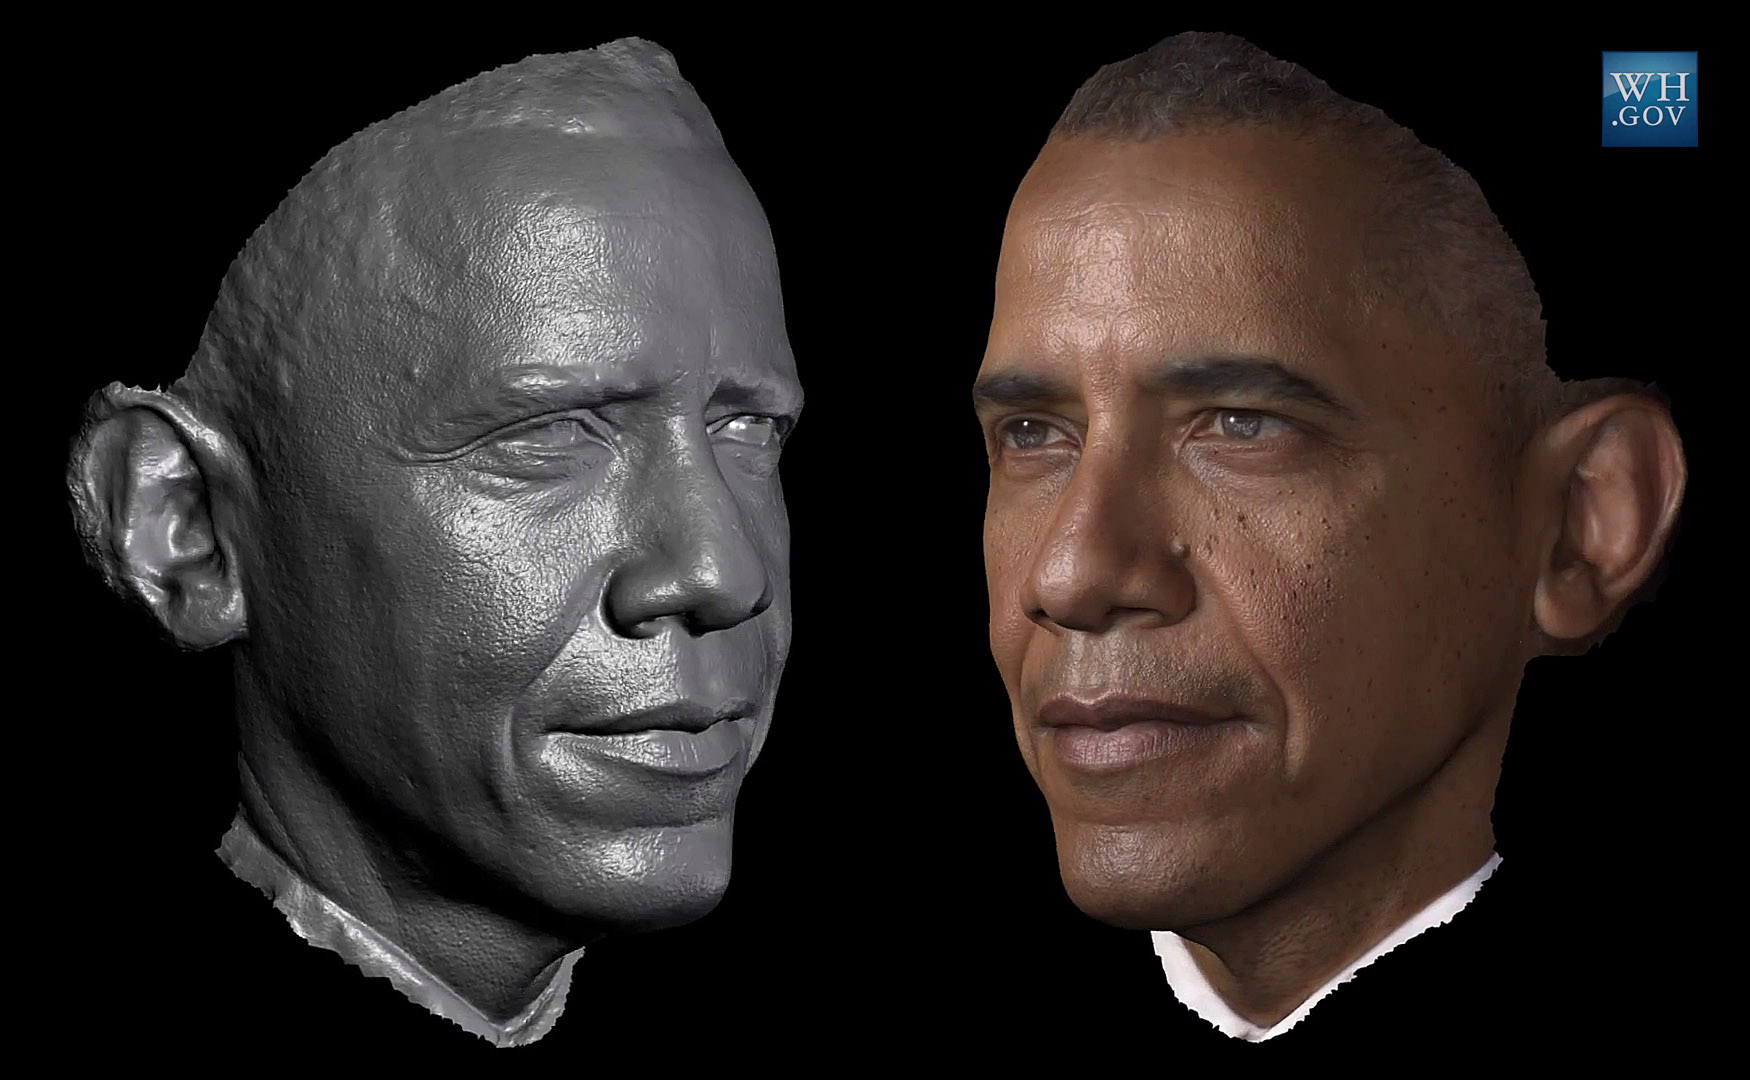
\includegraphics[height=5.8cm]{images/obama_scan}
% 		\caption{\small Minh họa công trình tái tạo khuôn mặt tổng thống Obama \cite{metallo2015scanning}}
% 		\label{fig:obamascan}
% 	\end{subfigure}
% 	\caption{Minh họa kỹ thuật đồ họa máy tính trong việc xây dựng người kỹ thuật số}
% 	\label{fig:DigitalHuman}
% \end{figure}

% Mỗi ngày, trên thế giới có hàng tỷ người nhìn vào màn hình RGB, kết quả hiển thị trên màn hình là đầu ra của mọi hệ thống phần mềm. Do đó, việc hiển thị từng pixel trên màn hình và cách để mô phỏng lại hình ảnh trên một cách chân thực nhất được các nhà khoa học về đồ họa máy tính (Computer Graphic) nghiên cứu từ những năm 1960s và đặc biệt là việc mô phỏng lại con người. Ngay từ năm 2014, các họa sĩ 3D đã có thể tạo nên một nhân vật người siêu thật như \autoref{fig:CGI} trong khi đó các phần cứng máy tính còn chưa phát triển như hiện nay. 

% Ngày nay, công nghệ đồ họa máy tính đã hoàn toàn có thể mô phỏng nhiều vật giống đến mức siêu thực (realistic), bao gồm các vật phức tạp như nước, đường xá, bánh mì,...  và thậm chí là cả cơ thể và khuôn mặt con người với độ chi tiết đến từng lông tơ, nốt mụn và vân mắt. 
% Vào năm 2015, bằng kỹ thuật quét 3 chiều ghi lại toàn bộ các góc của khuôn mặt, sự phản chiếu ánh sáng, trong công trình \cite{metallo2015scanning}
% các nhà khoa học đồ họa máy tính đã có thể tái tạo toàn bộ khuôn mặt của tổng thống Obama trên máy tính với độ chính xác cao và gần như không thể phân biệt \autoref{fig:obamascan}.

% Trí tuệ nhân tạo thể hiện kết quả vượt bậc những năm gần đây, không chỉ trong nghiên cứu mà còn trong ứng dụng thực tế, tiêu biểu như ứng dụng ChatGPT, MidJourney và sự phát triển cả theo chiều dọc và chiều ngang trong nhiều lĩnh vực ứng dụng trí tuệ nhân tạo. Mặc dù đồ họa máy tính đã có thể xây dựng khuôn mặt người siêu thật, việc sinh cử chỉ lại phụ thuộc vào việc chụp chuyển động (Motion Capture) từ các cảm biến và gặp khó khăn khi xây dựng hệ thống trí tuệ nhân tạo học từ dữ liệu.

% Các hệ thống trí tuệ nhân tạo hiện nay đã có thể tạo văn bản và giọng nói tiệm cận như con người, nhưng một trong những trở ngại lớn nhất để xây dựng con người kỹ thuật số hiện nay chính là việc sinh cử chỉ. Chính vì vậy, mục tiêu của luận văn là xây dựng một hệ thống sinh cử chỉ hội thoại dựa trên cảm xúc và ngữ nghĩa với dữ liệu đầu vào gồm cả văn bản và giọng nói.

% \section{Động lực nghiên cứu}

% Sinh cử chỉ hội thoại giúp ích cho rất nhiều lĩnh vực như hoạt ảnh, dựng phim, trò chơi điện tử, giáo dục và những ứng dụng thực tế ảo. Việc sinh cử chỉ chuyển động được thực hiện theo cách truyền thống là thuê các diễn viên sử dụng thiết bị theo dõi chuyển động và bố trí các hệ thống cảm biến xung quanh thu nhận chuyển động để đạt được độ chính xác chân thực nhất. Tuy nhiên, các chuyển động thu được sau đó chỉ được phát lại và không có sự biến đổi linh hoạt giữa các hành động. Do đó, việc áp dụng trí tuệ nhân tạo để có thể học các chuyển động từ dữ liệu thu nhận và sau đó có thể sinh ra dữ liệu mới sẽ là một cuộc cách mạng trong ngành công nghiệp chụp chuyển động.

% Vào năm 2011, một nhóm tác giả \cite{bergmann2011relation} đã chứng minh rằng có sự liên hệ giữa giọng nói và cử chỉ con người, đây chính là tiền đề cho thấy chúng ta có thể dùng dữ liệu giọng nói để có thể dùng để học và biểu diễn được cử chỉ con người.
% Với sự thành công của các mô hình ngôn ngữ tự nhiên trong xử lý văn bản và độ chính xác siêu thật trong việc mô phỏng gương mặt con người, ngành đồ họa máy tính đã đạt được những tiến bộ vượt bậc. Cùng với đó là sự dễ dàng và chính xác trong việc tổng hợp giọng nói con người.
% Việc ứng dụng trí tuệ nhân tạo để sinh cử chỉ con người là một trong những điểm nghẽn chính trong phát triển trợ lý ảo giao tiếp và tương tác với con người.

% \section{Dữ liệu bài toán}
% \label{sec:Data}


% \begin{figure}[H]
% 	\centering
% 	\begin{subfigure}{0.49\textwidth}
% 		\centering
% 		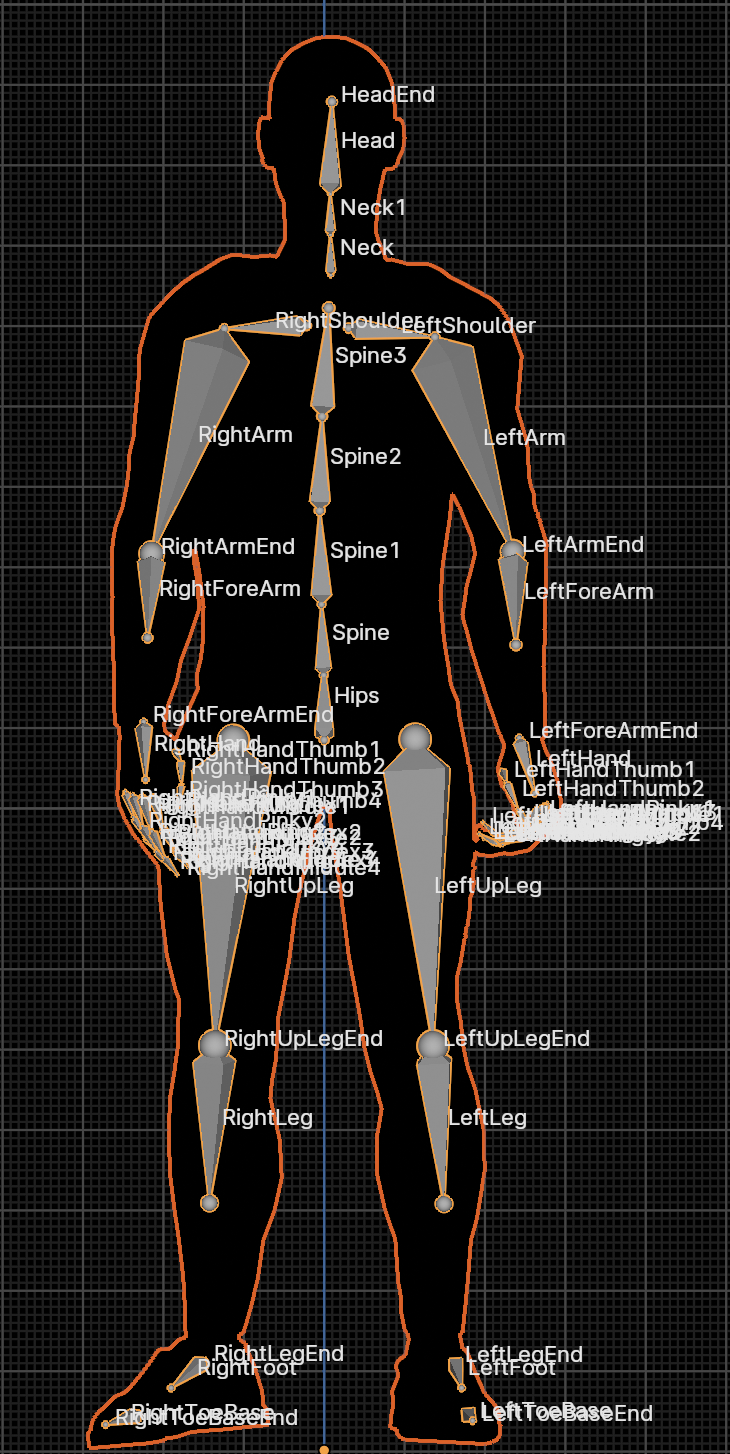
\includegraphics[height=10cm]{images/Skeleton.png}
% 		\caption{\small Khung xương và tên của các khớp của một khung xương trong mỗi khung hình.}
% 		\label{fig:Skeleton}
% 	\end{subfigure}
% 	\hfill
% 	\begin{subfigure}{0.49\textwidth}
% 		\centering
% 		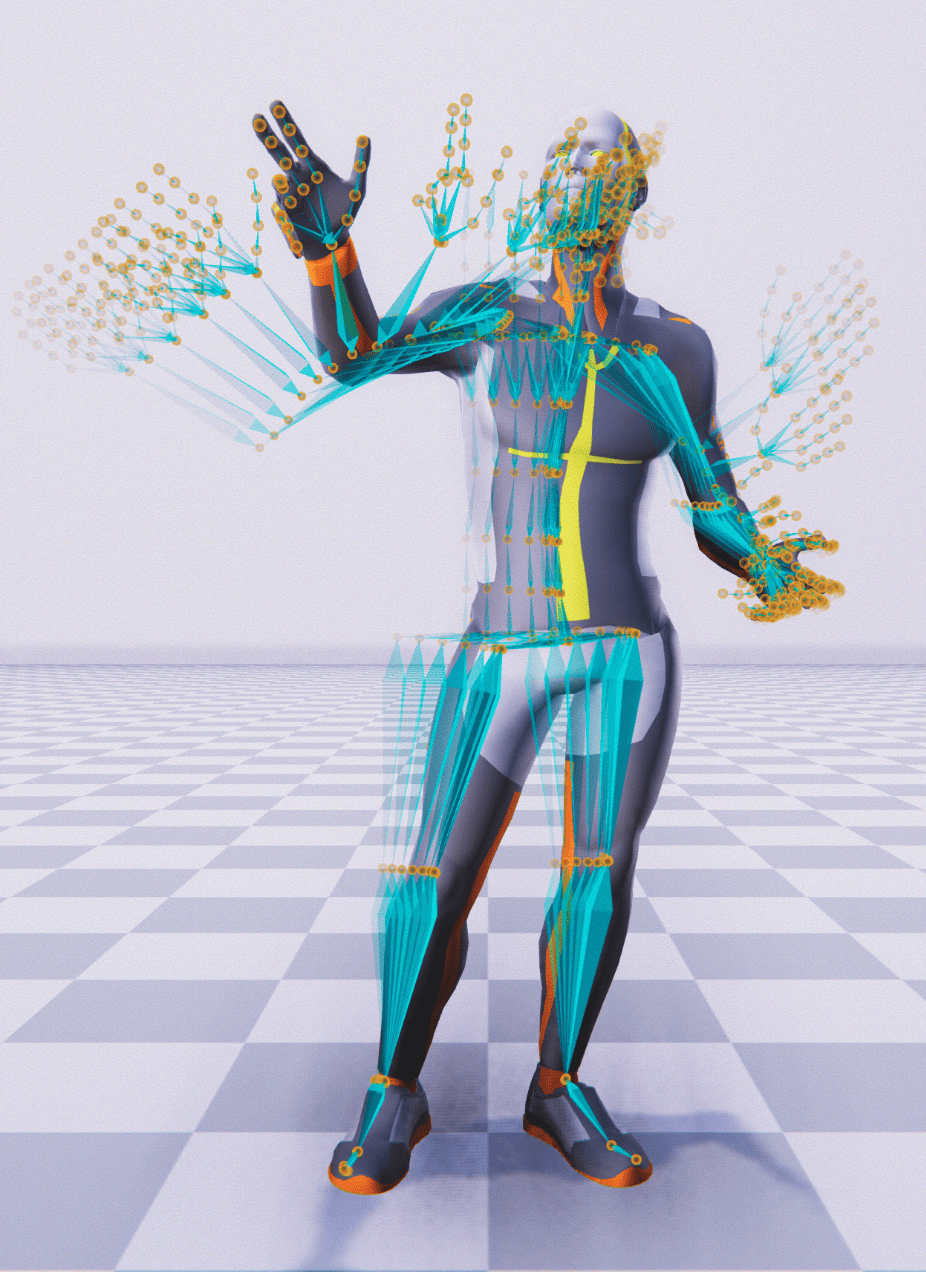
\includegraphics[height=10cm]{images/MotionPastAndFuture.png}
% 		\caption{\small Chuỗi chuyển động của cử chỉ bao gồm 6 cử chỉ quá khứ và 6 cử chỉ tương lai.}
% 		\label{fig:MotionPastAndFuture}
% 	\end{subfigure}
% \end{figure}

% \subsection{Kiến trúc khung xương của cử chỉ}

% Cử chỉ (gesture) trong luận văn là sự chuyển động của toàn bộ cơ thể của một nhân vật như hình \autoref{fig:Skeleton} theo từng khung hình. Để có thể biểu diễn các chuyển động của một nhân vật trong đồ họa máy tính, các chuyển động sẽ được biểu diễn thành chuyển động của các xương (bone) riêng lẻ. Bao gồm cánh tay (hand), chân (leg), đầu (head), xương sống (spine),... Kiến trúc đầy đủ của một nhân vật được trình bày ở phụ lục \autoref{appendix:BVHData:skeleton}.

% Dữ liệu một nhân vật theo thời gian trong thực tế sẽ được thu nhận bằng các hệ thống chụp chuyển động (motion capture) với các hệ thống camera và cảm biến chuyên biệt. Kết quả của quá trình motion capture là các tệp được định nghĩa dưới dạng tệp BVH (Biovision Hierarchy).

% Các tệp BVH bao gồm hai thành phần chính: {HIERARCHY} và {MOTION}. HIERARCHY được thể hiện dưới dạng một cây bao gồm các thông tin về tên và vị trí khởi tạo các khung xương, MOTION là dữ liệu về chuyển động của toàn bộ khung xương theo từng khung hình (frame).  Mỗi tệp BVH sẽ có thông tin về số khung hình trên giây ($\text{fps}$) và tổng sống khung hình. Thông tin mỗi tệp BVH được trình bày ở phụ lục \autoref{appendix:BVHData:BVHStructure}. 


% \subsection{Kiến trúc chuyển động của cử chỉ}

% Dữ liệu chuyển động của cử chỉ như \autoref{fig:MotionPastAndFuture} hay phần MOTION của tệp BVH sẽ chứa thông tin về tọa độ và góc quay của một nhân vật theo từng khung hình. Dữ liệu mỗi khung hình là tập khung xương (skeleton) bao gồm $75$ xương (bone), $\{ \textbf{b}_{1}, \textbf{b}_{2}, \cdots , \textbf{b}_{75} \}$, mỗi xương thể hiện vị trí (position) $\{ p_{x}, p_{y}, p_{z} \}$ và góc quay (rotation) $\{ r_{x}, r_{y}, r_{z} \}$ chuyển động của một nhân vật theo thời gian.

% Kết quả của việc sinh cử chỉ (gesture generation) là sinh ra chuỗi chuyển động góc quay các xương của nhân vật theo từng khung hình (frame). Việc sinh cử chỉ (gesture generation) được đánh giá bằng việc tạo ra các cử chỉ tự nhiên, giống con người (human-likeness) và phù hợp với ngữ cảnh.

% Trong luận văn, các dữ liệu về vị trí và góc quay của khung xương nhân vật được tiền xử lý để chuyển thành một vector đặc trưng $\mathbf{g} \in \mathbb{R}^{D}$ với $D=1141$. Dữ liệu cần học khi đó sẽ là $\bx \in \mathbb{R}^{M \times D}$.

% Quá trình xử lý dữ liệu được trình bày đầy đủ ở \autoref{appendix:BVHData}.

% \section{Phát biểu bài toán}
% \label{sec:ProblemStatement}

% Với kết quả cuối cùng là chuỗi cử chỉ thể hiện sự chuyển động của các khung xương theo từng khung hình, có thể áp dụng nhiều phương pháp khác nhau như phương pháp học phân loại (classification), gom nhóm (clustering), hồi quy (regression), .. Trong luận văn này, bài toán sinh cử chỉ được xem xét như một bài toán hồi quy (regression), với đầu vào là một chuỗi cử chỉ cho trước và đầu ra là chuỗi cử chỉ tiếp theo cần dự đoán.

% \begin{figure}[H]
% 	\centering
% 	\href{https://www.youtube.com/watch?v=B6nv1kQmi-Q}{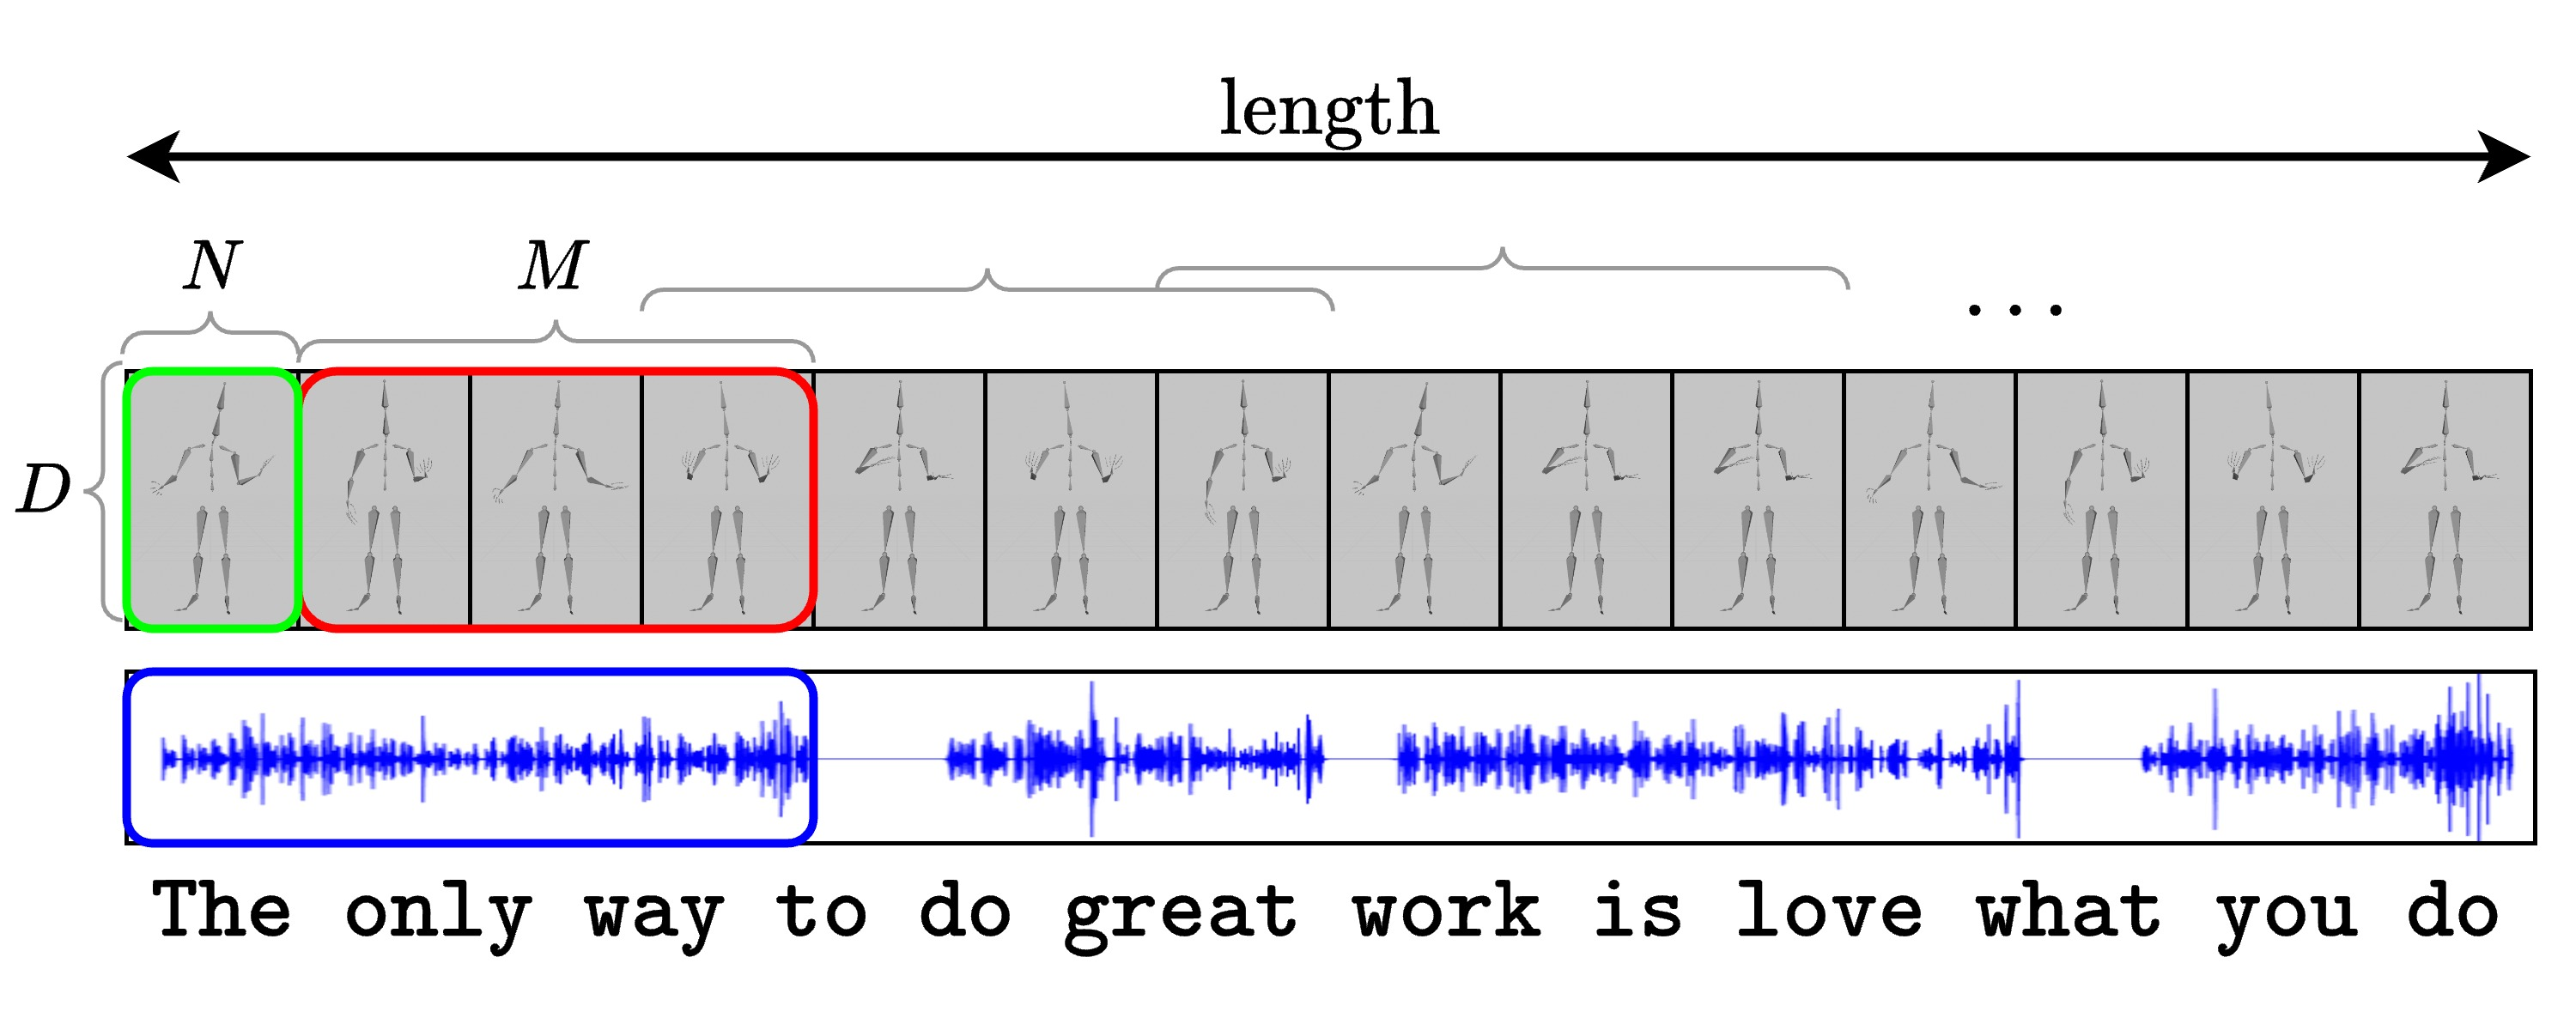
\includegraphics[width=\linewidth]{FeatureProcessing}}
% 	\caption{Minh họa một chuỗi cử chỉ, $N$ khung hình đầu được lấy làm cử chỉ khởi tạo $\mathbf{s}$ (seed gesture) và $M$ khung hình còn lại làm cử chỉ để học}
% 	\label{fig:GestureSeries}
% \end{figure}

% Với một chuỗi cử chỉ có độ dài khung hình bất kỳ, cảm xúc sẽ được gán cho toàn bộ chuỗi cử chỉ. Một điểm cải tiến của luận văn là tương ứng với chuỗi cử chỉ là dữ liệu giọng nói và đoạn văn bản được dịch từ dữ liệu giọng nói tương ứng.
% Mục tiêu của luận văn là xây dựng mô hình để dự đoán từng đoạn nhỏ, với thông tin dữ liệu đầu vào bao gồm chuỗi $N$ khung hình cử chỉ cho trước $\mathbf{s} \in \mathbb{R}^{1:N \times D}$ (seed gesture), chuỗi giọng nói $\mathbf{a}$ (speech), văn bản $\mathbf{v}$ (text),  cảm xúc $\mathbf{e}$ (emotion) tương ứng.

% Kết quả dự đoán của mô hình là $\hat{\mathbf{x}} \in \mathbb{R}^{1:M \times D}$ bao gồm từ khung hình 1 đến khung hình $M$ chuỗi cử chỉ tiếp theo . Với dữ liệu gốc là chuỗi cử chỉ đã có $\mathbf{x}  \in \mathbb{R}^{1:M \times D}$.

% \begin{multicols}{2}
	
% \textbf{Đầu vào}

% \begin{itemize}
% 	\item Chuỗi cử chỉ khởi tạo: $\mathbf{s} \in \mathbb{R}^{1:N \times D}$
% 	\item Chuỗi giọng nói: $\mathbf{a}$
% 	\item Văn bản: $\mathbf{v}$ 
% 	%				\in \mathbb{R}^{16000 M}
% 	%			trích xuất đặc trưng MFCC: $\mathbf{a} \in \mathbb{R}^{M \times C_{\text{mfcc}}}$
% 	\item Cảm xúc: $\mathbf{e}$ 
	
% 	{\small
% 		(\texttt{Happy},  \texttt{Sad},  \texttt{Neutral}, \texttt{Angry}, \texttt{Old}, \texttt{Funny})
% 	}
% \end{itemize}

% \columnbreak

% \textbf{Dữ liệu dự đoán}
% \vspace{-10pt}
% \begin{itemize}
% 	\item Chuỗi cử chỉ dự đoán: $\hat{\mathbf{x}} \in \mathbb{R}^{1:M \times D}$
% \end{itemize}

% \textbf{Dữ liệu gốc}
% \vspace{-10pt}
% \begin{itemize}
% 	\item Chuỗi cử chỉ gốc: $ \mathbf{x}  \in \mathbb{R}^{1:M \times D}$
% \end{itemize}

% \end{multicols}

% \section{Các khó khăn cần giải quyết}
% \label{sec:difficult}

% Có rất nhiều khó khăn trong việc xây dựng một mô hình có thể học được các đặc trưng cử chỉ hội thoại như con người.

% Thứ nhất, \textit{dữ liệu không đủ nhiều và chất lượng}, chi phí để tạo ra một bộ dữ liệu trong ngành công nghiệp chụp chuyển động có chất lượng và quy mô lớn để ứng dụng thực tế là rất cao.

% Thứ hai, \textit{sự thiếu đồng nhất về ngữ cảnh của các loại dữ liệu}, các bộ dữ liệu về văn bản thường nhiều hơn so với giọng nói, và cũng không rõ văn bản đó được tạo ra bởi ai. Sự đồng bộ giữa giọng nói và cảm xúc khi nói cũng thường thiếu trong tập dữ liệu. Ngoài ra, dữ liệu văn bản trong tập dữ liệu huấn luyện lại thuộc nhiều chủ đề đa dạng.
 
% Thứ ba, \textit{sự phân bố không cân xứng về  dữ liệu giữa các loại đặc trưng cần học}. Các dữ liệu dùng cho nghiên cứu cử chỉ hiện nay thường tập trung vào ngôn ngữ Tiếng Anh, các cử chỉ có sự phân bố không cân xứng giữa các trạng thái như nói, hỏi, hoặc im lặng.

% Thứ tư, \textit{chi phí tính toán với nhiều loại dữ liệu của mô hình là một thách thức lớn}. Với đầu vào của mô hình gồm nhiều loại dữ liệu như văn bản, tiếng nói và điểm 3D, cần nhiều lớp mã hóa cho từng loại dữ liệu, dẫn đến chi phí tính toán cao trong cả giai đoạn huấn luyện và suy luận. Nếu giảm thông tin dữ liệu đầu vào cũng sẽ giảm kết quả suy luận của mô hình khi sinh cử chỉ.

% Cuối cùng, \textit{các bước xử lý cần được thực hiện tuần tự}, cách hiệu quả nhất để con người tương tác với máy tính là thông qua giọng nói và nhập từ bàn phím, tuy nhiên việc xử lý được văn bản và giọng nói để làm đầu vào cho mô hình phải thực hiện tuần tự. Độ trễ trong quá trình suy luận của sản phẩm thực tế cũng là một vấn đề lớn, vì người dùng không thể chờ đợi quá lâu để nhận kết quả. Ngoài ra, việc hiển thị cử chỉ đó lên máy tính bằng kỹ thuật đồ họa cũng cần được tối ưu để giảm thời gian xử lý.


% \section{Đóng góp dự kiến}

% \begin{itemize}
% 	\item Dựa trên tập dữ liệu có sẵn, luận văn chuyển giọng nói trong tập dữ liệu thành văn bản, và dùng văn bản đó để làm dữ liệu huấn luyện mới như là một dữ liệu ngữ nghĩa bổ sung trong quá trình học.
	
% 	\item Dựa trên mô hình cơ bản DiffuseStyleGesture, luận văn mở rộng thêm đặc trưng văn bản trong quá trình khử nhiễu có điều kiện.
	
% 	\item Luận văn sử dụng Unity để render, trích xuất dữ liệu và trực quan hóa kết quả sinh cử chỉ.
	
% 	\item Luận văn xây dựng hệ thống kết xuất, và minh họa chương trình bằng Unity
% \end{itemize}


\chapter{INTRODUCTION}
\label{Introduction}

\section{General Background}

\begin{figure}[htbp]
	\centering
	\begin{subfigure}{0.35\textwidth}
		\centering
		
\includegraphics[height=5.8cm]{images/cgi}
		\caption{\small CGI technology with hyper-realistic digital humans \cite{edchrisjones}}
		\label{fig:CGI}
	\end{subfigure}
	\hfill
	\begin{subfigure}{0.6\textwidth}
		\centering
		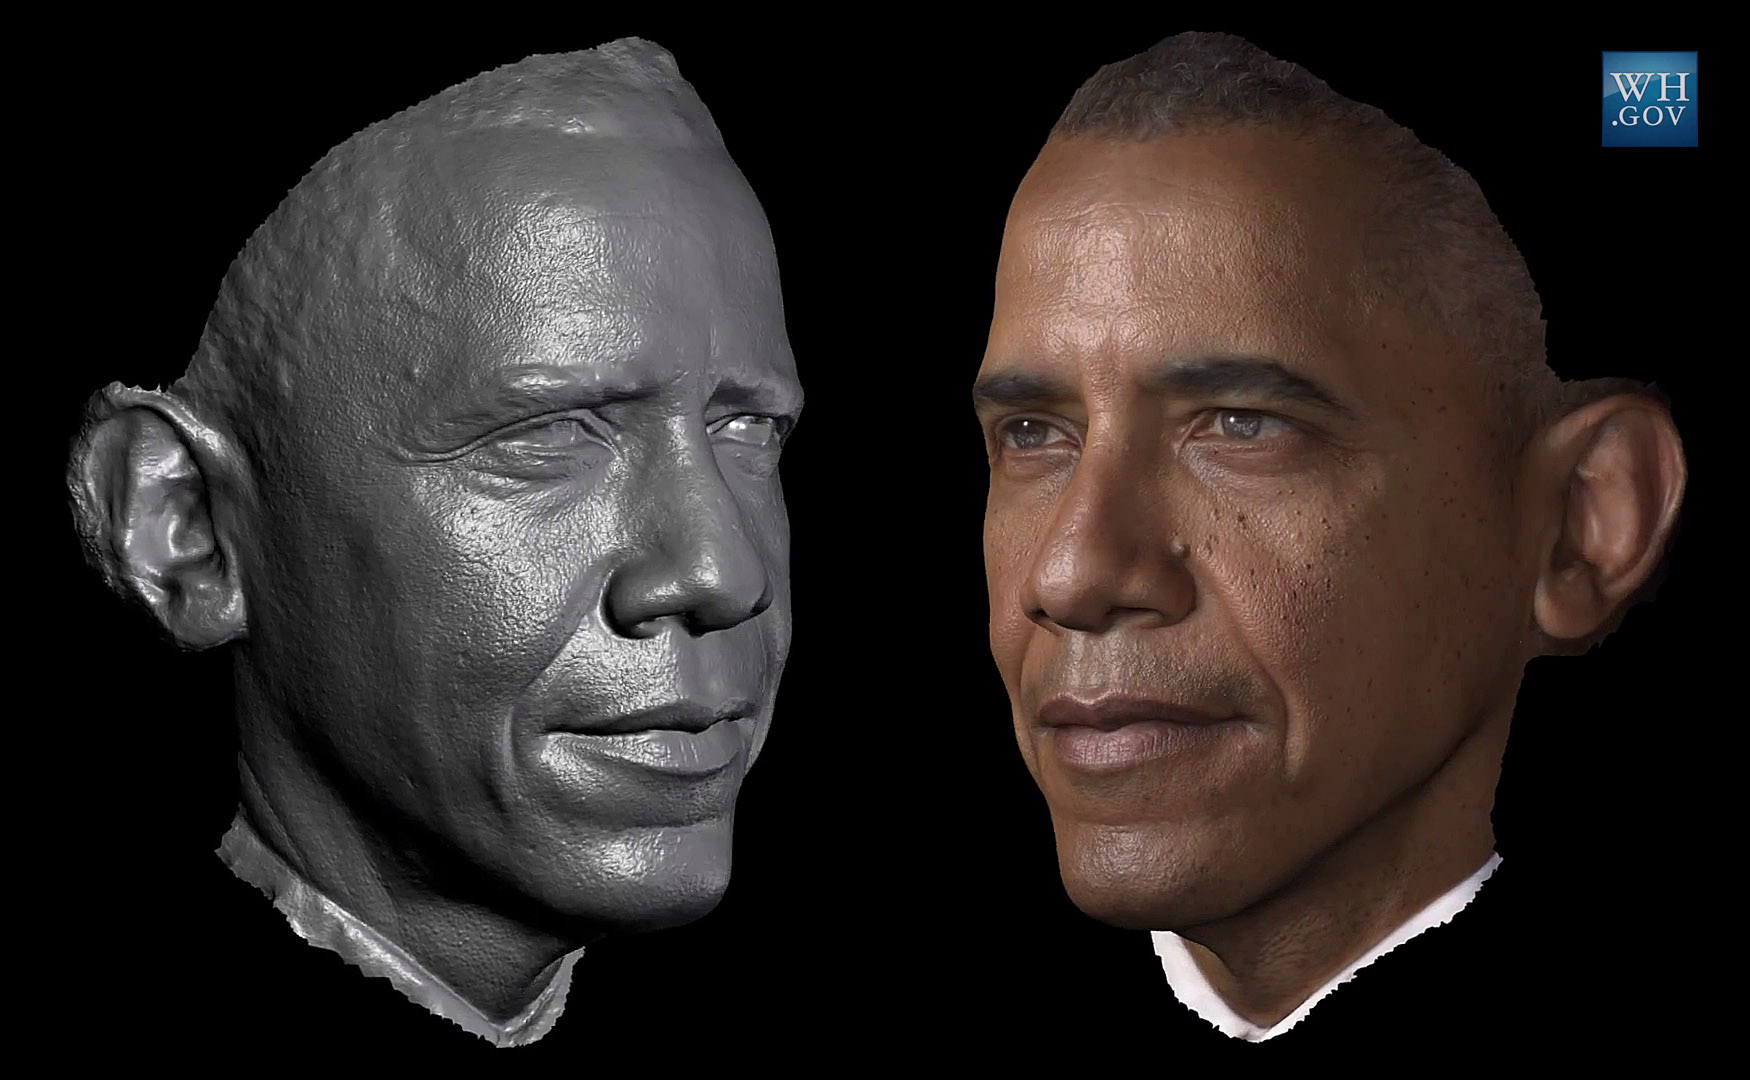
\includegraphics[height=5.8cm]{images/obama_scan}
		\caption{\small Illustration of the reconstruction of President Obama's face \cite{metallo2015scanning}}
		\label{fig:obamascan}
	\end{subfigure}
	\caption{Illustration of computer graphics techniques in constructing digital humans}
	\label{fig:DigitalHuman}
\end{figure}

Every day, billions of people around the world look at RGB screens, where the display results are outputs of various software systems. Thus, pixel-level rendering on the screen and how to simulate it most realistically has been a topic of computer graphics research since the 1960s, especially the simulation of humans. As early as 2014, 3D artists were able to create hyper-realistic digital characters like in \autoref{fig:CGI}, even when computing hardware was not as advanced as today.

Today, computer graphics technology is capable of simulating many objects to a hyper-realistic level, including complex ones like water, roads, bread, and even the human body and face down to fine details such as pores, acne, and eye patterns. In 2015, using 3D scanning techniques to capture all facial angles and light reflections, researchers in \cite{metallo2015scanning} managed to reconstruct the entire face of President Obama on a computer with high accuracy and near-indistinguishability (\autoref{fig:obamascan}).

Artificial intelligence (AI) has made remarkable advances in recent years, not only in research but also in real-world applications, such as ChatGPT, MidJourney, and across many vertical and horizontal domains. While computer graphics can now construct hyper-realistic faces, generating gestures still relies heavily on motion capture using sensors, and building AI systems that can learn from data remains challenging.

Modern AI systems can now generate human-like text and speech. However, one of the biggest obstacles in building digital humans is gesture generation. Therefore, the aim of this thesis is to build an emotional and semantic-conditioned conversational gesture generation system using both text and speech as input.

\section{Research Motivation}

Conversational gesture generation benefits many fields such as animation, filmmaking, video games, education, and virtual reality applications. Traditionally, gesture motion is captured by hiring actors equipped with motion tracking devices and surrounding sensors to record movements with high realism. However, these recorded motions are replayed statically and lack flexibility between actions. Therefore, applying AI to learn motion from data and generate new motions will be a revolution in the motion capture industry.

In 2011, a group of researchers \cite{bergmann2011relation} demonstrated a correlation between human speech and gestures, forming the foundation to learn and represent gestures from speech data. With the success of natural language models in text processing and the hyper-realistic simulation of human faces, computer graphics has achieved significant progress. Combined with the ease and accuracy of human speech synthesis, gesture generation through AI has become one of the main bottlenecks in developing interactive virtual assistants.

\section{Problem Data}
\label{sec:Data}

\begin{figure}[H]
	\centering
	\begin{subfigure}{0.49\textwidth}
		\centering
		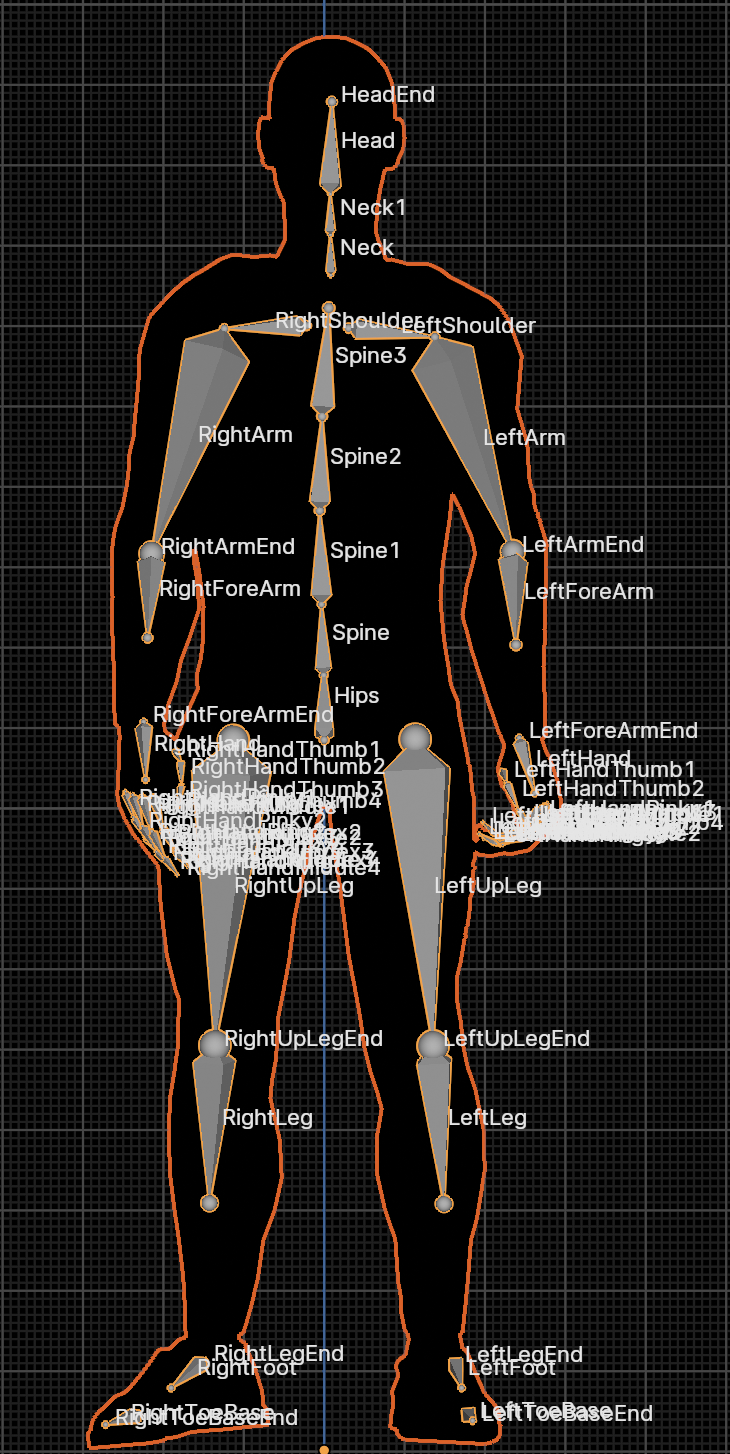
\includegraphics[height=10cm]{images/Skeleton.png}
		\caption{\small Skeleton and joint names of a frame}
		\label{fig:Skeleton}
	\end{subfigure}
	\hfill
	\begin{subfigure}{0.49\textwidth}
		\centering
		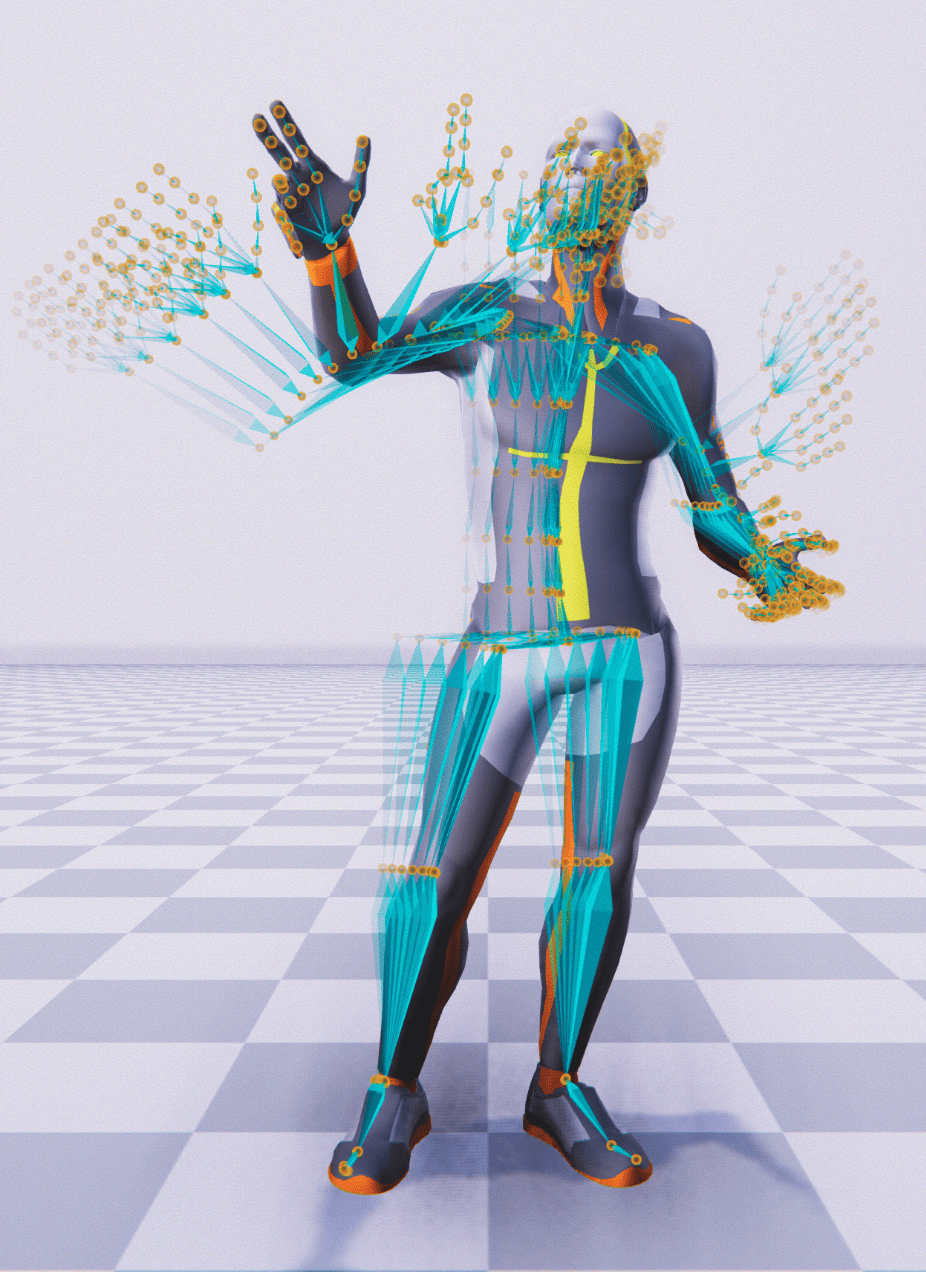
\includegraphics[height=10cm]{images/MotionPastAndFuture.png}
		\caption{\small Motion sequence consisting of 6 past and 6 future gestures}
		\label{fig:MotionPastAndFuture}
	\end{subfigure}
\end{figure}

\subsection{Skeleton Structure of Gestures}

In this thesis, a gesture is defined as the movement of a character's entire body over time, as shown in \autoref{fig:Skeleton}, captured frame by frame. In computer graphics, character motion is represented as bone-specific movements, including hands, legs, head, spine, etc. The full character skeleton structure is presented in Appendix \autoref{appendix:BVHData:skeleton}.

Motion data is captured via motion capture systems using cameras and specialized sensors. The output is typically stored in BVH (Biovision Hierarchy) files.

A BVH file consists of two main parts: `HIERARCHY` and `MOTION`. The `HIERARCHY` section is structured as a tree containing the skeleton’s initial positions and names. The `MOTION` section contains the movement data for the entire skeleton frame-by-frame. Each BVH file includes frame rate (fps) and total frame count. Details are presented in Appendix \autoref{appendix:BVHData:BVHStructure}.

\subsection{Motion Structure of Gestures}

Gesture motion data, as illustrated in \autoref{fig:MotionPastAndFuture}, or the `MOTION` section of a BVH file, contains position and rotation information per frame. Each frame is a skeleton of 75 bones: $\{ \textbf{b}_{1}, \textbf{b}_{2}, \cdots , \textbf{b}_{75} \}$, where each bone has position $\{ p_{x}, p_{y}, p_{z} \}$ and rotation $\{ r_{x}, r_{y}, r_{z} \}$.

The output of gesture generation is a sequence of bone rotations per frame. The generated gestures are evaluated based on naturalness, human-likeness, and contextual appropriateness.

In this thesis, the skeleton’s position and rotation data are preprocessed into a feature vector $\mathbf{g} \in \mathbb{R}^{D}$ with $D = 1141$. The learning data becomes $\bx \in \mathbb{R}^{M \times D}$. The preprocessing pipeline is detailed in \autoref{appendix:BVHData}.

\section{Problem Statement}
\label{sec:ProblemStatement}

The ultimate goal is to produce a sequence of gestures that reflect the motion of the skeleton frame by frame. This can be approached via classification, clustering, or regression. In this thesis, gesture generation is framed as a regression problem: given an input gesture sequence, predict the next sequence.

\begin{figure}[H]
	\centering
	\href{https://www.youtube.com/watch?v=B6nv1kQmi-Q}{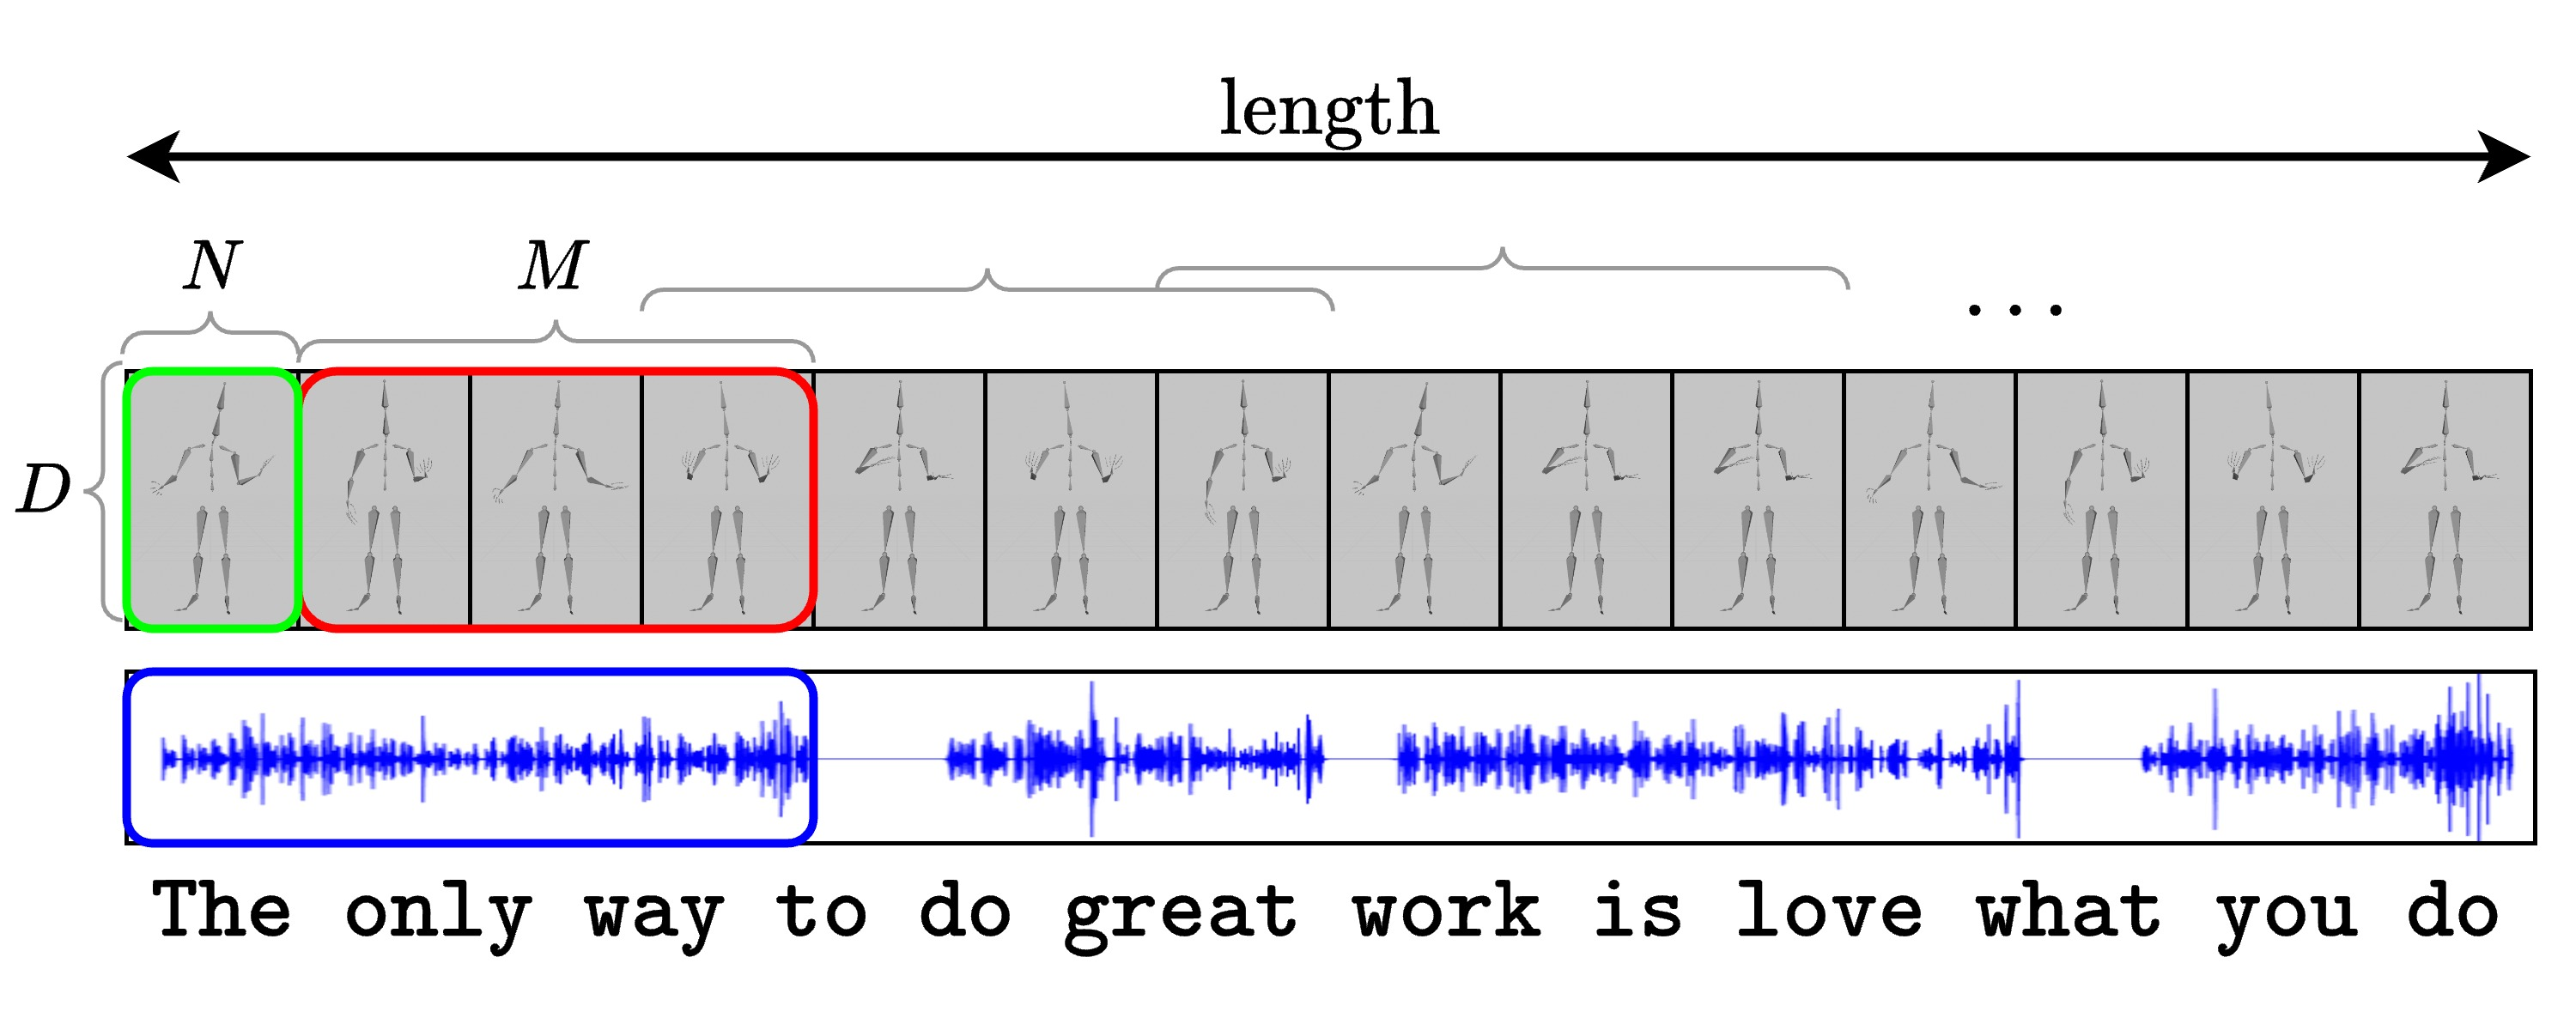
\includegraphics[width=\linewidth]{FeatureProcessing}}
	\caption{A gesture sequence: the first $N$ frames are used as seed gesture $\mathbf{s}$, and the remaining $M$ frames are to be predicted}
	\label{fig:GestureSeries}
\end{figure}

Each gesture sequence is labeled with an emotion. A key novelty of this thesis is pairing the gesture sequence with both the original speech and the corresponding text (transcribed from the speech).

The objective is to build a model that predicts $M$ future frames from the given inputs: seed gesture $\mathbf{s} \in \mathbb{R}^{1:N \times D}$, speech $\mathbf{a}$, text $\mathbf{v}$, and emotion $\mathbf{e}$.

The model prediction is $\hat{\mathbf{x}} \in \mathbb{R}^{1:M \times D}$, which is compared against ground-truth gesture $\mathbf{x} \in \mathbb{R}^{1:M \times D}$.

\begin{multicols}{2}
	
\textbf{Input}

\begin{itemize}
	\item Seed gesture sequence: $\mathbf{s} \in \mathbb{R}^{1:N \times D}$
	\item Speech signal: $\mathbf{a}$
	\item Text: $\mathbf{v}$
	\item Emotion: $\mathbf{e}$ 
	
	{\small
		(\texttt{Happy},  \texttt{Sad},  \texttt{Neutral}, \texttt{Angry}, \texttt{Old}, \texttt{Funny})
	}
\end{itemize}

\columnbreak

\textbf{Predicted Output}
\vspace{-10pt}
\begin{itemize}
	\item Predicted gesture sequence: $\hat{\mathbf{x}} \in \mathbb{R}^{1:M \times D}$
\end{itemize}

\textbf{Ground Truth}
\vspace{-10pt}
\begin{itemize}
	\item Ground truth gesture: $ \mathbf{x}  \in \mathbb{R}^{1:M \times D}$
\end{itemize}

\end{multicols}

\section{Challenges}
\label{sec:difficult}

There are several challenges in building a model that can learn human-like conversational gesture patterns:

1. \textit{Limited and low-quality data:} Creating large-scale, high-quality datasets for motion capture is extremely costly in the industry.

2. \textit{Inconsistent context between modalities:} Text datasets are more abundant than speech, and speaker attribution is often missing. Synchronization between speech and emotional tone is also lacking. Additionally, training texts span many unrelated topics.

3. \textit{Imbalanced feature distributions:} Current datasets are biased toward English-speaking gestures, with imbalanced gesture distributions between speaking, questioning, and silent states.

4. \textit{High computational cost due to multimodal input:} The model must encode text, speech, and 3D pose data, increasing the computational load during both training and inference. Reducing input information also degrades performance.

5. \textit{Sequential preprocessing steps:} Although human-computer interaction is most effective through speech and keyboard input, processing the text and speech input for gesture generation must be done sequentially. In real-world applications, inference latency is critical, and users cannot wait long. Rendering the gestures on screen must also be optimized for speed.

\section{Expected Contributions}

\begin{itemize}
	\item From existing datasets, speech is transcribed into text and used as additional semantic features for training.
	
	\item Based on the DiffuseStyleGesture model, the thesis extends the conditional denoising process to include text features.
	
	\item The thesis uses Unity for rendering, data extraction, and visualization of gesture generation results.
	
	\item The thesis develops a rendering pipeline and demonstrates the system with Unity.
\end{itemize}



\chapter{TỔNG QUAN}
\label{Chapter2}

Bài toán sinh cử chỉ cũng tương tự như các bài toán khác, đều đã nghiên cứu và phát triển song hành với các phương pháp học máy truyền thống và hiện đại. Gồm các nhóm phương pháp dựa trên luật và các phương pháp dựa trên dữ liệu.  Đầu tiên luận văn trình bày về các đặc điểm của cử chỉ \autoref{sec:relationspeechandgesture}, từ đó là tiền đề cho việc học mối quan hệ giữa cử chỉ, văn bản và giọng nói. Trong mục \autoref{sec:commonstage}, luận văn sẽ trình bày về các công đoạn chung trong các phương pháp sinh cử chỉ.
Ở phần \autoref{sec:relatedwork}, luận văn trình bày về các phương pháp đã được sử dụng trong quá trình sinh cử chỉ. Luận văn sẽ so sánh các phương pháp, từ đó nêu lý do luận văn sử dụng mô hình diffusion để áp dụng cho bài toán sinh cử chỉ.
Trong phần \autoref{sec:diffusionbase}, luận văn sẽ trình bày về cách các mô hình diffusion được áp dụng cho bài toán sinh cử chỉ gần đây.

\section{Đặc điểm của cử chỉ}
\label{sec:relationspeechandgesture}

Theo ngôn ngữ học, cử chỉ có thể được phân thành 6 nhóm chính: cử chỉ thích nghi (adaptors), cử chỉ biểu tượng (emblems), cử chỉ chỉ định (deictics), cử chỉ biểu trưng (iconics), cử chỉ ẩn dụ (metaphorics), và cử chỉ nhấn mạnh (beat) \cite{ekman1969repertoire}, \cite{sebeok2011advances}. Trong số đó, cử chỉ nhấn mạnh không mang ý nghĩa ngữ nghĩa trực tiếp nhưng đóng vai trò quan trọng trong việc đồng bộ nhịp điệu giữa giọng nói và cử chỉ \cite{kipp2005gesture}, \cite{sebeok2011advances}. Tuy nhiên, nhịp điệu giữa giọng nói và cử chỉ nhấn mạnh không hoàn toàn đồng bộ, khiến việc học mối quan hệ thời gian giữa chúng trở nên phức tạp \cite{mcclave1994gestural}, \cite{bhattacharya2021speech2affectivegestures}, \cite{kucherenko2020gesticulator}, \cite{yoon2020speech}.

Cử chỉ tương tác với các cấp độ thông tin khác nhau trong giọng nói \cite{sebeok2011advances}. Chẳng hạn, cử chỉ biểu tượng, như hành động giơ ngón cái, thường liên quan đến thông tin ngữ nghĩa cấp cao (ví dụ: "tốt" hoặc "tuyệt vời"), trong khi cử chỉ nhấn mạnh thường đi kèm với thông tin cấp thấp như nhấn mạnh trong âm thanh. Các nghiên cứu trước đây thường chỉ sử dụng đặc trưng từ lớp cuối cùng của bộ mã hóa giọng nói để tổng hợp cử chỉ \cite{alexanderson2020style}, \cite{bhattacharya2021speech2affectivegestures}, \cite{kucherenko2021large}, \cite{qian2021speech}, \cite{yoon2022genea}. Tuy nhiên, cách tiếp cận này có thể làm trộn lẫn thông tin từ nhiều cấp độ, dẫn đến khó khăn trong việc phân tách rõ ràng nhịp điệu và ngữ nghĩa.

Như các nghiên cứu ngôn ngữ học chỉ ra \cite{kipp2005gesture}, \cite{neff2008gesture}, \cite{webb1997linguistic}, cử chỉ trong giao tiếp hàng ngày có thể được chia thành một số lượng giới hạn các đơn vị ngữ nghĩa với các biến thể chuyển động khác nhau. Dựa trên giả định này, được phân tách đặc trưng giọng nói thành hai loại: đặc trưng cấp cao đại diện cho các đơn vị ngữ nghĩa, và đặc trưng cấp thấp xác định các biến thể chuyển động. Từ đó, mối liên hệ giữa chúng được học thông qua các lớp khác nhau của bộ mã hóa giọng nói. Các thử nghiệm chứng minh rằng cơ chế này có khả năng tách biệt rõ ràng các đặc trưng ở nhiều cấp độ, đồng thời tổng hợp được cử chỉ phù hợp về ngữ nghĩa và phong cách.



\section{Tổng quan các phương pháp cho bài toán sinh cử chỉ}
\label{sec:relatedwork}

\subsection{Phương pháp dựa trên luật}

\subsubsection{Nguyên lý chung}

Dựa trên việc xây dựng các quy tắc hoặc luật rõ ràng, các quy tắc được định nghĩa thủ công, xác định cách hệ thống xử lý đầu vào để tạo ra đầu ra.

\subsubsection{Phương pháp}

Tiêu biểu cho phương pháp dựa trên luật là \textit{Robot behavior toolkit} \cite{huang2012robot} và  \textit{Animated conversation} \cite{cassell1994animated}.
Phương pháp dựa trên luật thường ánh xạ (mappings) từng giọng nói với từng đơn vị cử chỉ, với các luật được tạo thủ công. Phương pháp dựa trên luật thì dễ dàng điều khiển kết quả của mô hình và có khả năng giải thích tốt kết quả dự đoán của mô hình.
Tuy nhiên chi phí để tạo thủ công là không khả thi để xây dựng cho các ứng dụng phức tạp đòi hỏi phải xử lý một lượng dữ liệu rất lớn.

\subsection{Phương pháp dựa trên thống kê}

\subsubsection{Nguyên lý chung}

Dựa vào phân tích dữ liệu, học từ các mẫu trong tập dữ liệu và sử dụng các mô hình xác suất hoặc hàm toán học để đưa ra dự đoán. Phương pháp này dựa trên việc tối ưu hóa các tham số của mô hình để phù hợp với dữ liệu.

\subsubsection{Phương pháp}

Tương tự như phương pháp dựa trên luật, phương pháp dựa trên dữ liệu cũng ánh xạ các đặc trưng của giọng nói tương ứng với cử chỉ nhưng thay vì làm thủ công thì được sử dụng học một cách tự động dựa trên các phân tích thống kê của dữ liệu.

Tiêu biểu của phương pháp thống kê là \textit{Gesture controllers} \cite{levine2010gesture}, \textit{Statistics-based} \cite{yang2020statistics}, các phương pháp này sử dụng phân phối xác suất để tìm sự tương đồng giữa các đặc trưng giọng nói và cử chỉ. \textit{Gesture modeling}  \cite{neff2008gesture} xây dựng mô hình xác suất để học từng phong cách của từng người nói.

\subsection{Phương pháp học sâu}

\textbf{Nguyên lý chung của phương pháp học sâu}

Sử dụng mạng nơ-ron đa lớp (Multi-layer Perceptron) để tự động trích xuất đặc trưng từ dữ liệu thô và học các biểu diễn phức tạp của dữ liệu. Mô hình học thông qua tối ưu hóa các tham số.

\begin{figure}[H]
	\centering
	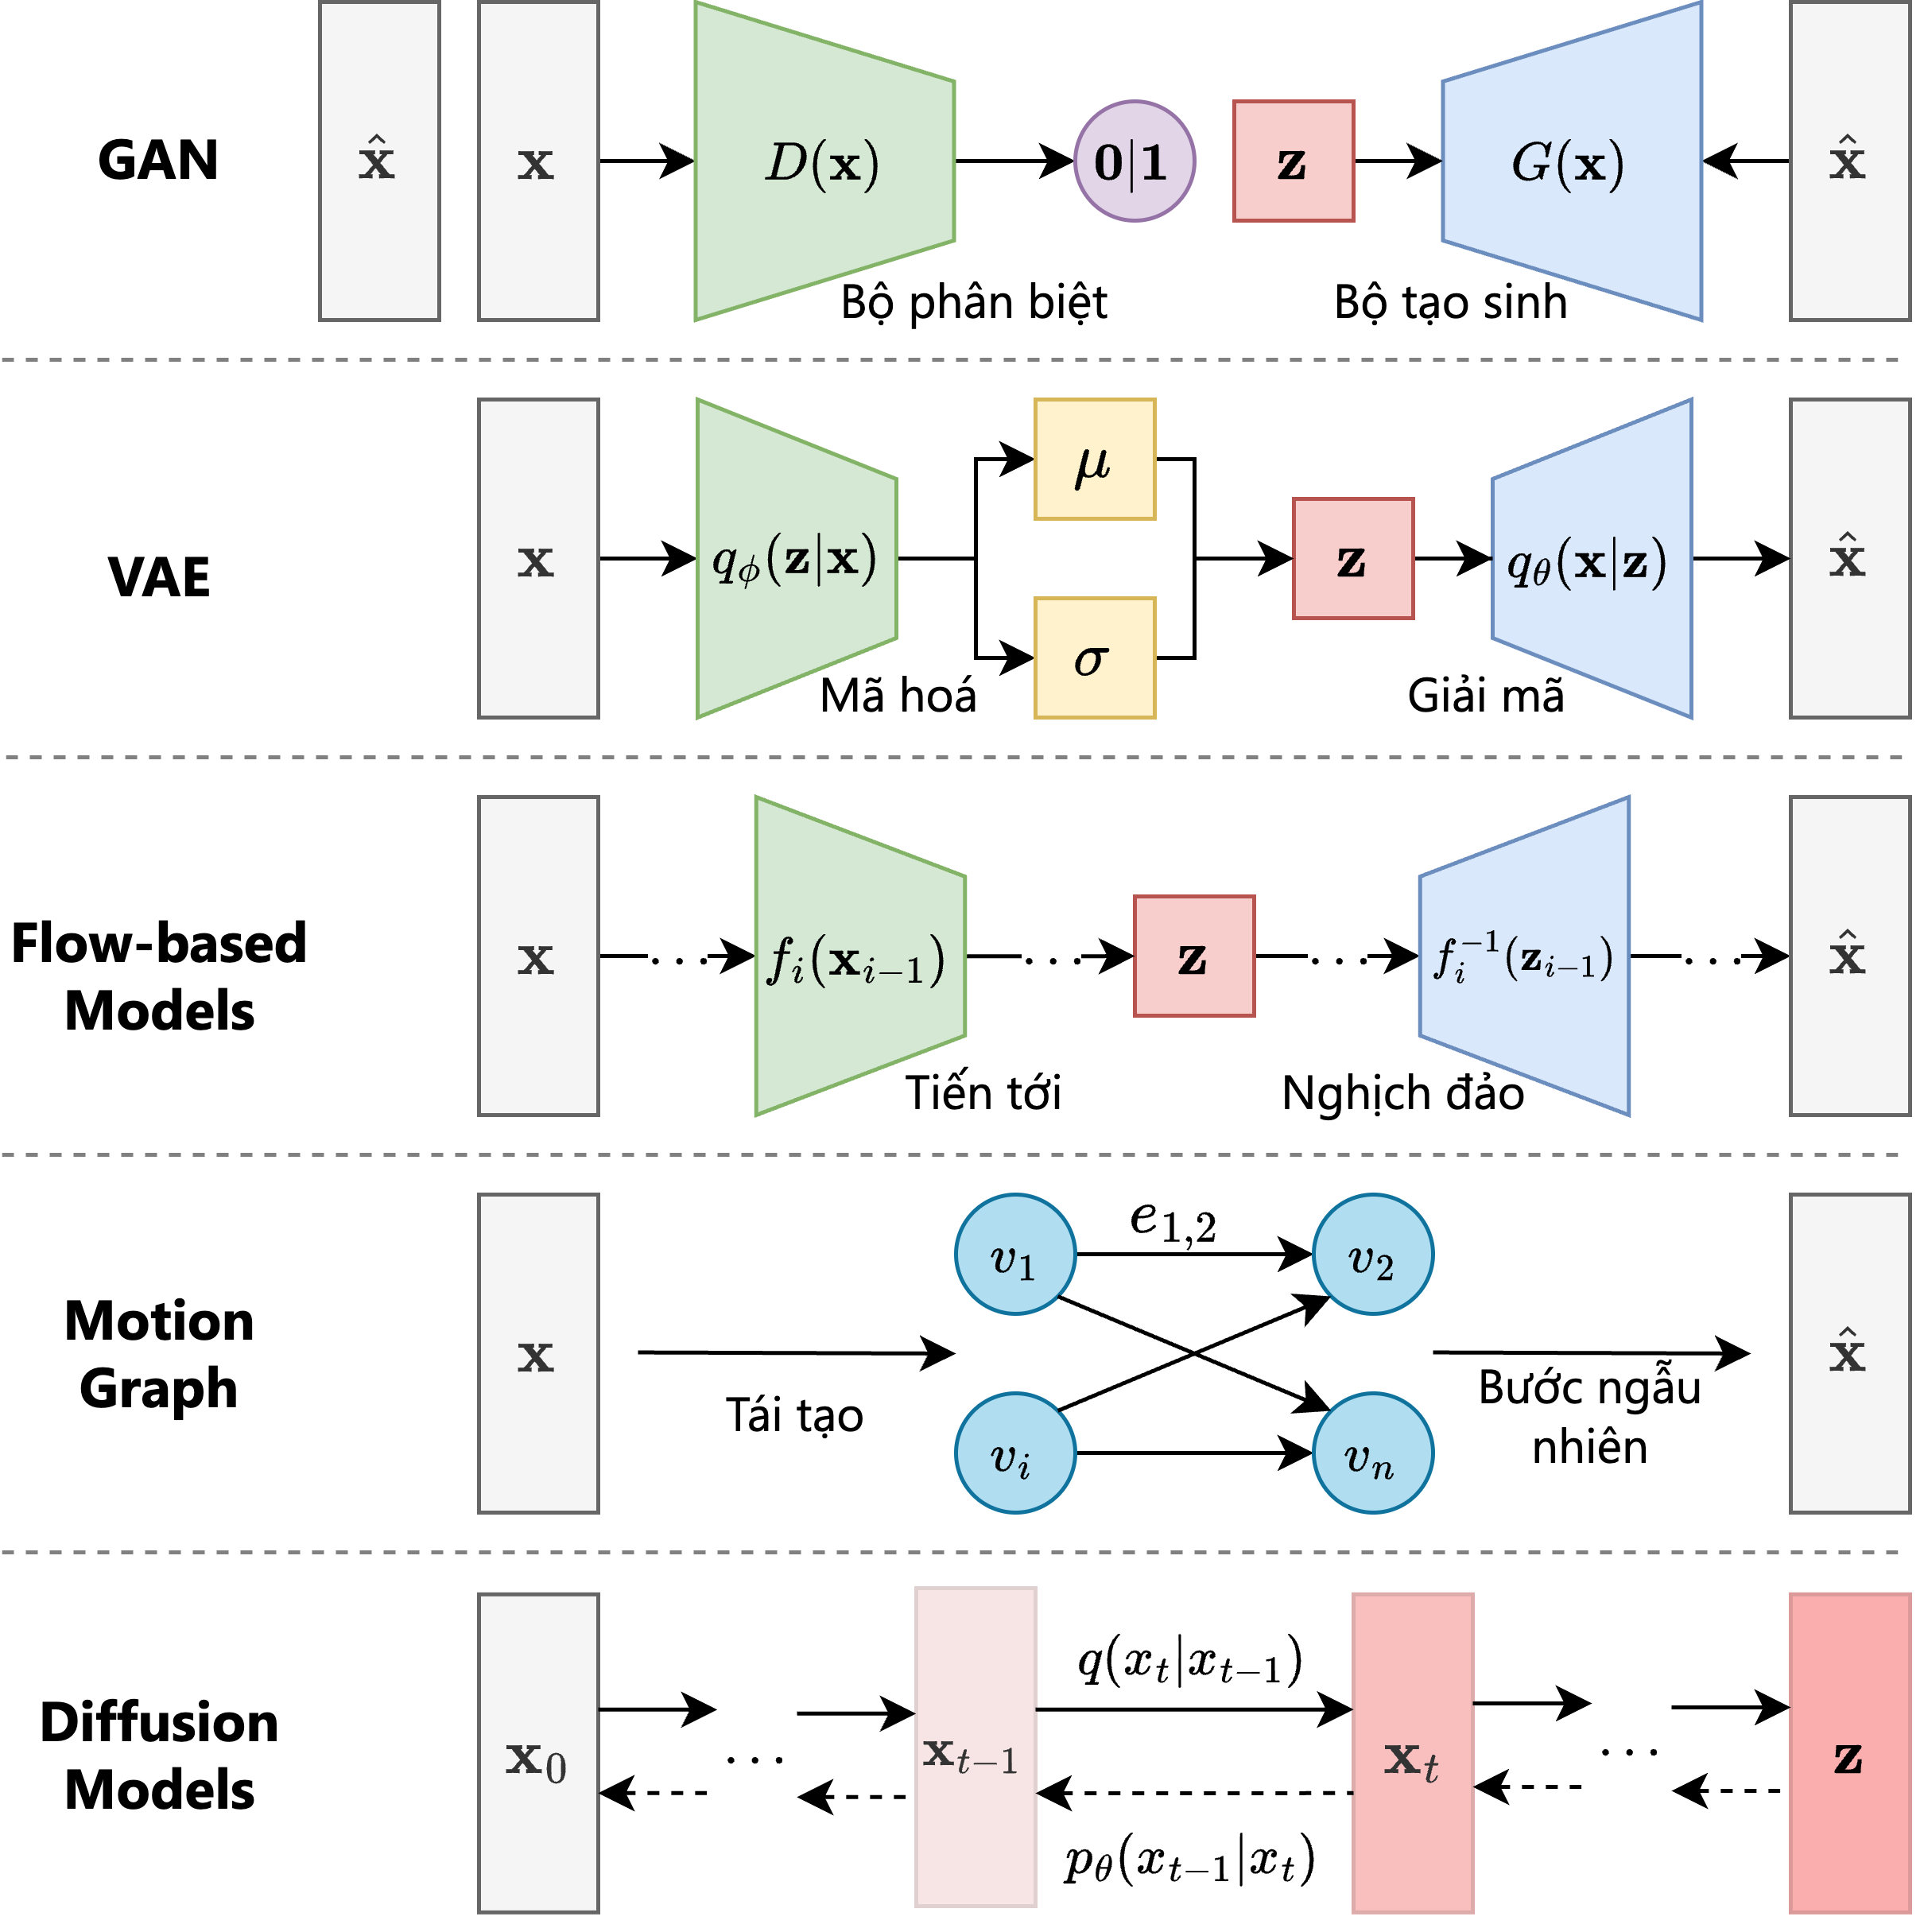
\includegraphics[width=0.8\textwidth]{GeneralOverview}
	\caption{Tổng quan về các mô hình tạo sinh khác nhau.}
	\label{fig:GeneralOverview}
\end{figure}

Phương pháp sinh cử chỉ bằng học sâu minh họa ở \autoref{fig:GeneralOverview} được chia thành hai nhóm chính: học dựa trên ước lượng log likelihood (likelihood-based model)  và phương pháp dựa vào các mô hình sinh ngầm định (implicit generative models) \cite{song2021score}.

\subsubsection{Mô hình dựa trên likelihood}

\textbf{Nguyên lý chung của mô hình dựa trên likelihood}

Mô hình dựa trên Log Likelihood hoạt động bằng cách tối đa hóa xác suất hợp lý của dữ liệu quan sát được, dựa trên các tham số $\theta$ của mô hình. Mục tiêu là tìm được tham số tối ưu $\theta'$ dựa trên xác suất $p(\mathbf{x})$ của dữ liệu, trong đó $\mathbf{x}$ là dữ liệu chuỗi cử chỉ.

\textbf{Phương pháp}

Quá trình áp dụng các phương pháp học sâu vào bài toán sinh cử chỉ cũng tương đồng với sự phát triển của các phương pháp học sâu, từ RNN, LSTM và Transformer .v.v.. Các phương pháp tiêu biểu trong nhóm phương pháp dựa trên likelihood:

\begin{itemize}[]
	\item Phương pháp \textit{Gesticulator} \cite{kucherenko2020gesticulator} sử dụng kiến trúc Multilayer Perceptron (MLP) để mã hóa đặc trưng văn bản và âm thanh, sử dụng vector văn bản từ BERT làm vector đặc trưng cho văn bản. 
	
	\item Trong \textit{HA2G} \cite{liu2022learning} dựa trên kiến trúc Transformer xây dựng một mô hình phân cấp (hierarchical) để học các tương quan ở nhiều cấp độ giữa lời nói và cử chỉ, từ các đặc trưng cục bộ (local) đến toàn cục (global). 
	
	\item \textit{Gesture Generation from Trimodal Context} \cite{yoon2020speech} dựa trên kiến trúc RNN, coi việc sinh cử chỉ là bài toán dịch trong xử lý ngôn ngữ. 
	
	\item \textit{DNN} \cite{chiu2015predicting} sử dụng LSTM kết hợp GRU để xây dựng mô hình phân loại (classifier neural network) từng đơn vị cử chỉ để chọn một đơn vị cử chỉ phù hợp dựa trên đầu vào là giọng nói. 
	
	\item \textit{Cascaded Motion Network (CaMN)} \cite{liu2022beat} đề xuất tập dữ liệu BEAT đồng thời đề xuất mô hình giống như thác nước, các thông tin về người nói, nhãn cảm xúc, văn bản, giọng nói và cử chỉ được đi qua các lớp để trích xuất đặc trưng để được các vector tiềm ẩn. Trong giai đoạn kết hợp các đặc trưng, mô hình CaMN kết hợp các đặc trưng theo hình thác nước, lần lượt kết hợp các đặc trưng người nói và cảm xúc, và tiếp tục kết hợp với các vector tiềm ẩn của văn bản, giọng nói và cử chỉ.
	
	\item \textbf{Motion Graph} : Trong phương pháp \textit{Gesturemaster} \cite{zhou2022gesturemaster}, mô hình xây dựng đồ thị ngữ nghĩa, từ trong câu được kết nối trong một đồ thị, nơi các liên kết biểu thị quan hệ ngữ nghĩa giữa chúng. Dựa trên thông tin đồ thị, mô hình chọn các đỉnh (node) và cạnh (edges) có sự tương đồng nhất để biểu diễn cử chỉ. 
	
\end{itemize}

\subsubsection{Mô hình sinh ngầm định}
\label{sec:ImplicitGenerativeModels}

\textbf{Nguyên lý}

Mô hình sinh ngầm định học phân phối dữ liệu mà không cần biểu diễn tường minh hàm mật độ xác suất $p(\bx)$. Thay vì trực tiếp tính xác suất $p(\bx)$, mô hình sẽ học một ánh xạ $G_{\theta}: \mathcal{Z} \to \mathcal{X}$ thông qua so khớp phân phối giữa dữ liệu thật và dữ liệu sinh ra $\mathbf{x} = G_\theta(\mathbf{z}), \quad \mathbf{z} \sim p_z(\mathbf{z})$.  Trong đó $\mathcal{Z}$ là không gian nhiễu đầu vào, thường có phân phối đơn giản \(p_{z}\) (ví dụ: Gaussian, Uniform). \(\mathcal{X}\) là không gian dữ liệu thực, là chuỗi cử chỉ \(\mathbf{x}\). 

Trong bài toán sinh cử chỉ, để kết hợp thêm các điều kiện về giọng nói, nhãn văn bản, các mô hình sinh ngầm định thường kết hợp thêm điều kiện $\mathbf{c}$, với điều kiện là ngữ cảnh của bài toán để có được kết quả sinh: $\mathbf{x} = G_\theta(\mathbf{z}, \mathbf{c})$. Ngữ cảnh của bài toán có thể bao gồm giọng nói, văn bản, mã định danh người nói, phong cách, cảm xúc hay cử chỉ khởi tạo.

%
Ví dụ tiêu biểu nhất là mô hình generative adversarial networks (GANs) và Diffusion. Khi dữ liệu được tổng hợp bằng cách chuyển phân phối dữ liệu ban đầu ở dạng phân phối chuẩn về phân phối của dữ liệu.

\textbf{Phương pháp} 

Các phương pháp tiêu biểu cho mô hình sinh ngầm định là 

\begin{itemize}
	\item \textit{MoGlow} \cite{henter2020moglow} sử dụng Normalizing Flows được sử dụng để duy trì tính nhất quán và tính tương thích của chuyển động, đồng thời cung cấp khả năng điều khiển thông qua các thông số đầu vào. Điều này cho phép người dùng tạo ra các chuyển động mới hoặc thay đổi các chuyển động hiện có bằng cách thay đổi các thông số điều khiển.
	
	\item \textbf{GAN}: \textit{GRU-based WGAN} \cite{wu2021probabilistic} sử dụng Wasserstein GAN để đánh giá và cải thiện chất lượng của việc tổng hợp cử chỉ, mô hình tập trung vào việc tối ưu hóa hàm mất mát Wassserstein, giúp giảm tình trạng chảy đặc (mode collapse) thường gặp trong GAN truyền thống. GRU được sử dụng để xử lý dữ liệu lời nói và biến nó thành các đặc trưng cử chỉ có thể sử dụng được. Sau đó, những đặc trưng này được cung cấp vào mạng WGAN, nơi chúng sẽ được đánh giá và tinh chỉnh để tổng hợp cử chỉ.
	
	\item \textbf{VAE}:  \textit{FreeMo} \cite{xu2022freeform} sử dụng VAE để phân rã (decomposing) các cử chỉ thành tư thế cử chỉ (pose modes) và giai điệu chuyển động (rhythmic motions). Tư thế cử chỉ được sinh ra ngẫu nhiên sử dụng quá trình lấy mẫu có điều kiện trong không gian ẩn của VAE. Trong khi các giai điệu chuyển động được sinh ra từ 
	
	\item \textbf{VQ-VAE} \textit{Rhythmic Gesticulator} \cite{ao2022rhythmic} tiền xử lý các đoạn giọng nói theo nhịp điệu (beats) để tách giọng nói thành các đoạn nhỏ, và biểu diễn chúng thành các khối theo kích thước chuẩn hóa (normalization). Tương tự phương pháp VQ-VAE, các chuỗi cử chỉ đã chuẩn hóa sẽ được lượng tử hóa (quantization) thành các vùng không gian khác nhau của cử chỉ được gọi là các từ vựng cử chỉ (gesture lexicon). Mô hình học từ vựng cử chỉ (gesture lexicon) từ khối chuẩn hóa trên với điều kiện là cử chỉ trước đó, phong cách cử chỉ và giọng nói. Sau đó mô hình tái tạo lại từ quá trình chuẩn hóa (denormalization) để có được chuỗi cử chỉ ban đầu. Khác với mô hình sinh ngầm định như GANs hay Diffusion, VQ-VAE thường tập trung vào việc nén dữ liệu hơn là sinh dữ liệu trực tiếp.
	
	\item \textbf{Diffusion}:  Mô hình Diffusion tập trung vào việc tạo ra dữ liệu mới từ trạng thái nhiễu, phục hồi ngược lại dữ liệu gốc. Các phương pháp dựa trên Diffusion sẽ được trình bày ở mục \autoref{sec:diffusionbase}
	
\end{itemize}


\subsection{So sánh các phương pháp sinh cử chỉ}

\begin{table}[H]
	\small
	\centering
	\renewcommand{\arraystretch}{1.5} % Tăng khoảng cách giữa các hàng
	\resizebox{\textwidth}{!}{ % Giảm kích thước bảng để vừa với trang
		\begin{tabular}{|p{0.2\textwidth}|p{0.35\textwidth}|p{0.35\textwidth}|p{0.2\textwidth}|}
			\hline
			\textbf{Phương pháp tiêu biểu} & \textbf{Ưu điểm} & \textbf{Nhược điểm} & \textbf{Loại phương pháp} \\ \hline
			Robot behavior toolkit \cite{huang2012robot} & 
			- Dễ hiểu và dễ triển khai. \newline 
			- Dễ giải thích và có thể kiểm soát được \newline
			- Hiệu quả trong các trường hợp đơn giản hoặc dữ liệu nhỏ. & 
			- Không tổng quát hóa tốt với dữ liệu phức tạp. \newline 
			- Đòi hỏi nhiều công sức trong việc xây dựng quy tắc thủ công. & 
			Mô hình dựa trên luật  \\ \hline
			MLP \cite{kucherenko2020gesticulator}, RNN \cite{bhattacharya2021speech2affectivegestures}, \cite{liu2022learning}, \cite{hasegawa2018evaluation}, \cite{yoon2020speech}, CNN \cite{habibie2021learning}, Transformer \cite{bhattacharya2021text2gestures}  & 
			- Khả năng ước lượng mật độ xác suất của dữ liệu \newline 
			- Có khả năng mở rộng và học từ dữ liệu lớn & 
			- Dễ bị ảnh hưởng bởi nhiễu \newline 
			- Kết quả thấp ở vùng dữ liệu hiếm \newline
			- Khả năng sinh không đa dạng & 
			Mô hình dựa trên Likelihood \\ \hline
			\textbf{DiffusionStyle-Gesture} \cite{yang2023diffusestylegesture}, MDM \cite{tevet2022human}, Motiondiffuse \cite{zhang2022motiondiffuse} &
			- Tạo ra dữ liệu chất lượng cao. \newline 
			- Linh hoạt và đa dạng \newline
			- Phủ được vùng có mật độ dữ liệu thấp & 
			- Cần cấu hình phức tạp để đạt hiệu năng tốt. \newline 
			- Mỗi lần lấy nhiễu ngẫu nhiên là khác nhau. \newline 
			- Quá trình lấy mẫu chậm & 
			Mô hình sinh ngầm định\\ \hline
		\end{tabular}
	}
	\caption{Bảng so sánh ưu và nhược điểm của các phương pháp}
	\label{table:CompareMethod}
\end{table}

%\textbf{Bảng so sánh các phương pháp}
%
%\begin{table}[ht]
%	\centering
%	\begin{tabular}{|l|l|l|l|l|l|}
%		\hline
%		\textbf{Phương pháp} & \textbf{Loại mô hình} & \textbf{Đặc điểm nổi bật} & \textbf{Ưu điểm} & \textbf{Hạn chế} & \textbf{Tài liệu tham khảo} \\ \hline
%		VAE  & Autoencoder & Biểu diễn dữ liệu trong không gian tiềm ẩn & Tạo đặc trưng ẩn & Khó kiểm soát đầu ra & \cite{kingma2013auto} \\ \hline
%		VQ-VAE & Autoencoder (cải tiến) & Dùng codebook cho không gian tiềm ẩn & Biểu diễn chi tiết hơn & Phức tạp hơn & \cite{van2017neural} \\ \hline
%		RNN & Mạng hồi tiếp & Xử lý chuỗi dữ liệu & Tốt cho dữ liệu tuần tự & Khó huấn luyện & \cite{bhattacharya2021speech2affectivegestures} \\ \hline
%		Transformer & Mạng chú ý & Tạo cử chỉ qua cơ chế chú ý & Hiệu quả với dữ liệu dài & Yêu cầu nhiều tài nguyên & \cite{bhattacharya2021text2gestures} \\ \hline
%		WGAN & GAN & Học phân phối dữ liệu đối kháng & Tạo sự đa dạng & Khó huấn luyện & \cite{wu2021probabilistic} \\ \hline
%		Normalizing Flow & Mô hình xác suất & Học phân phối phức tạp & Hữu ích với dữ liệu phức tạp & Cần tài nguyên tính toán lớn & \cite{alexanderson2020style} \\ \hline
%		Diffusion Models & Mô hình sinh dữ liệu & Chi tiết cao, xử lý dữ liệu thiếu & Tạo cử chỉ chi tiết & Thời gian huấn luyện lâu & \cite{xu2022freeform} \\ \hline
%	\end{tabular}
%	\caption{So sánh các phương pháp sinh cử chỉ}
%\end{table}

\section{Công đoạn chung của phương pháp học sâu trong bài toán sinh cử chỉ}
\label{sec:commonstage}

Như đã trình bày ở \autoref{sec:Data}, cử chỉ bao gồm chuỗi chuyển động của tọa độ điểm 3D. Với mỗi tập dữ liệu số lượng xương (bone) mỗi khung hình sẽ khác nhau. 

Cách tiếp cận bằng học sâu với bài toán sinh cử chỉ (gesture generation) được thực hiện với nhiều phương pháp khác nhau. Tuy nhiên luận văn tổng quát hóa lại thành các công đoạn chính như \autoref{fig:CommonStage} sau:

\begin{figure}[H]
	\centering
	\includegraphics[width=\textwidth]{CommonStage}
	\caption{Các công đoạn trong mô hình sinh cử chỉ.}
	\label{fig:CommonStage}
\end{figure}

\begin{enumerate}[label=\textbf{\arabic*.}]
	\item \textbf{Tiền xử lý dữ liệu} (Preprocessing): Trong công đoạn tiền xử lý, các dữ liệu về đoạn giọng nói, dữ liệu về chuỗi cử chỉ, đoạn văn bản sẽ được đọc, số hóa để thu được các vector hoặc ma trận thể hiện thông tin thô của dữ liệu. Đối với mỗi phương pháp học khác nhau, các thông tin dữ liệu ban đầu sẽ được chọn để học cũng khác nhau.
	
	\item \textbf{Xử lý đặc trưng} (Feature Processing): Trong công đoạn xử lý đặc trưng, các dữ liệu thô như giọng nói và văn bản được nhúng (embedding) để biểu diễn thành các vector đặc trưng. Các phương pháp khác nhau sẽ chọn các mô hình nhúng khác nhau. Việc biểu diễn các cử chỉ của nhân vật thành các vector đặc trưng của mỗi phương pháp cũng khác nhau.
	
	\item \textbf{Trích xuất đặc trưng} (Feature Extraction): Công đoạn trích xuất đặc trưng sẽ dùng các lớp biến đổi tuyến tính (linear) hoặc các lớp CNN để trích xuất các đặc trưng của dữ liệu. Các dữ liệu về văn bản hoặc giọng nói sau khi xử lý đặc trưng có thể cũng được cho đi qua các lớp trích xuất đặc trưng để biểu diễn thành các vector đặc trưng để biểu diễn tương ứng với văn bản và giọng nói.
	
	\item \textbf{Mã hóa đặc trưng} (Feature Encoding): Trong công đoạn mã hóa đặc trưng, các vector về cử chỉ, cảm xúc, và giọng nói sẽ được biểu diễn lên không gian tiềm ẩn nhỏ hơn kích thước ban đầu nhằm thuận tiện cho việc tính sự tương quan giữa các đặc trưng ở công đoạn kết hợp đặc trưng.
	
	\item \textbf{Kết hợp đặc trưng} (Feature Fusion): Trong công đoạn kết hợp đặc trưng, các đặc trưng giọng nói, văn bản, cử chỉ cũng như các thông tin khác được kết hợp với nhau bằng việc concat, các lớp kết nối đầy đủ hoặc kết hợp các đặc trưng bằng cách cộng hoặc trừ các vector tiềm ẩn.
	
	\item \textbf{Giải mã đặc trưng} (Feature Decoding): Trong công đoạn giải mã đặc trưng, các vector tiềm ẩn sẽ được giải mã hay tăng chiều dữ liệu về kích thước ban đầu.
	
	\item \textbf{Kết xuất} (Render): Sau khi có được vector ở kích thước ban đầu, các vector sẽ được biến đổi ngược trở về các tệp BVH để được kết xuất thông qua các phần mềm như Blender hoặc Unity để minh họa các chuyển động nhân vật.
\end{enumerate}

\section{Diffusion-base Model}
\label{sec:diffusionbase}

\subsection{Nguyên lý chung của các phương pháp dựa trên Diffusion}

\begin{figure}[H]
	\centering
	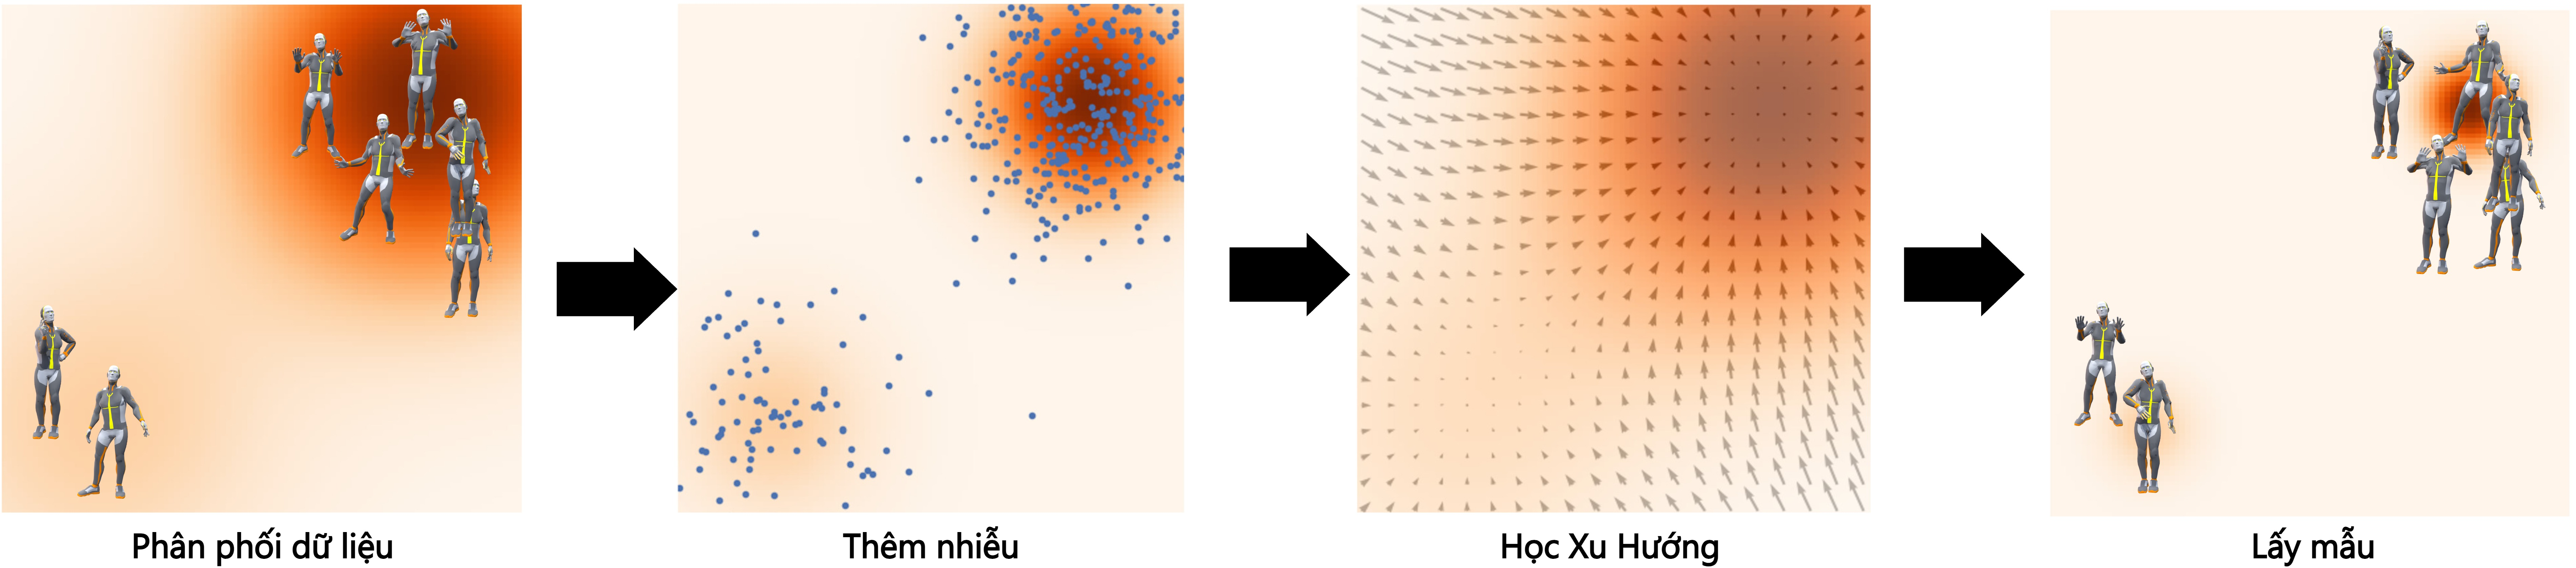
\includegraphics[width=\textwidth]{ScoreMatching}
	\caption{Minh họa nguyên lý chung của mô hình mô hình Diffusion.}
	\label{fig:ScoreMatching}
\end{figure}

Tương tự phương pháp trong nhóm phương pháp sinh ngầm định (Implicit Generative Models \autoref{sec:ImplicitGenerativeModels}), nguyên lý của mô hình Diffusion là học một hàm $f_{\theta}$ biểu diễn xu hướng (drift) của quá trình từ phân phối chuẩn $\mathcal{N}(0, \mathbf{I})$ về phân phối của dữ liệu $\bx_{0} \sim p(\bx)$, từ đó lấy mẫu (sampling) lên từng bước của quá trình đảo ngược để sinh ra các dữ liệu mới như \autoref{fig:ScoreMatching}.
Quá trình này được thực hiện từng $T$ bước, với nhiễu được thêm trong quá trình lấy mẫu giảm dần để mô hình có thể điều hướng về các vùng có mật độ dữ liệu lớn.

\subsection{Phương pháp tiêu biểu}
\label{subsec:TypicalMethod}

\subsubsection{Phương pháp tiêu biểu}

\begin{itemize}
	\item \textit{MotionDiffuse} \cite{zhang2022motiondiffuse} sử dụng mô hình Diffusion có điều kiện, với điều kiện dựa trên là văn bản mà không bao gồm âm thanh. Ngoài ra mô hình dự đoán nhiễu, chứ không dự đoán chuỗi cử chỉ gốc. Mô hình MotionDiffuse sử dụng các lớp Self-Attention và Cross Attention để tính tương quan giữa đặc trưng văn bản và đặc trưng cử chỉ trong công đoạn \textit{5. Kết hợp đặc trưng} (\autoref{fig:CommonStage}).
	
	\item \textit{Flame} \cite{kim2023flame} sử dụng mô hình diffusion với kiến trúc transformer. Trong công đoạn \textit{2. Xử lý đặc trưng} (\autoref{fig:CommonStage}), mô hình sử dụng mô hình pre-train RoBERTa để nhúng (embedding) văn bản để được các vector đặc trưng văn bản, và sử dụng chúng làm điều kiện cho mô hình. 
	Trong công đoạn \textit{5. Kết hợp đặc trưng} (\autoref{fig:CommonStage}), sử dụng văn bản làm token $\texttt{CLS}$ đầu tiên của chuỗi cử chỉ trước khi đi qua lớp Transformer Decoder .  Mô hình cũng dự đoán nhiễu đã được thêm vào mô hình Diffusion chứ không dự đoán chuỗi cử chỉ gốc.
	
	\item \textit{DiffWave} \cite{kong2020diffwave} sử dụng mô hình Diffusion với việc dự đoán nhiễu, các bước thời gian được đi qua nhiều lớp Fully Connected khác nhau và lớp kích hoạt Swish trước khi kết hợp các đặc trưng. Mô hình sử dụng kiến trúc dilated convolutions kế thừa từ WaveNet. Mô hình DiffWave giúp biểu diễn giọng nói được biểu diễn tốt hơn, tạo đầu vào hiệu quả hơn cho mô hình Diffusion.
	
	\item \textit{Listen, denoise, action} \cite{alexanderson2022listen} kế thừa từ mô hình DiffWave \cite{kong2020diffwave}, thay lớp dilated convolutions bằng Transformer , kết hợp với Conformers giúp cải thiện hiệu suất của mô hình.
	
	\item \textit{DiffSHEG} \cite{chen2024diffsheg} sử dụng mô hình diffusion, trong công đoạn \textit{2. Xử lý đặc trưng}, mô hình DiffSHEG sử dụng HuBERT để biểu diễn âm thanh. Coi biểu cảm là tín hiệu cho cử chỉ. Mô hình đạt được sự kết hợp thời gian thực của đồng thời cả biểu cảm khuôn mặt (facial expression) và cử chỉ (gesture).
	
	\item \textit{GestureDiffuCLIP} \cite{ao2023gesturediffuclip} sử dụng mô hình Diffusion với điều kiện là văn bản, GestureDiffuCLIP sử dụng phương pháp học tương phản (Contrastive Learning) để kết hợp đặc trưng văn bản thông qua CLIP để điều khiển phong cách của cử chỉ. Tương tự các phương pháp trên, coi văn bản như là Prompt của các mô hình sinh văn bản như StableDiffusion, Midjourney giúp mô hình học được cử chỉ từ đoạn văn bản mô tả.
	
	\item \textit{Freetalker} \cite{yang2024freetalker} sử dụng mô hình Diffusion để huấn luyện trên nhiều tập dữ liệu khác nhau, tạo cử chỉ cho người nói dựa trên lời nói và văn bản. Mô hình dự đoán cử chỉ gốc. Thay vì sử dụng Transformer, Freetalker sử dụng Attention-based Network để tính tương quan giữa các đặc trưng văn bản, âm thanh và cử chỉ trong công đoạn \textit{5. Kết hợp đặc trưng} (\autoref{fig:CommonStage}).
\end{itemize}


\subsubsection{Phương pháp được kế thừa trong luận văn}

\begin{itemize}
	\item \textit{MDM} \cite{tevet2022human}  áp dụng Diffusion có điều kiện cho bài toán sinh cử chỉ, với điều kiện là CLIP (Contrastive Language–Image Pre-training) của văn bản mô tả. MDM sử dụng kiến trúc transformer để tái tạo dữ liệu cử chỉ ban đầu, sử dụng Diffusion có điều kiện với điều kiện là đoạn văn bản mô tả chuyển động của cử chỉ. Tương tự các phương pháp diffusion sử dụng văn bản mô tả, trong công đoạn \textit{3. Trích xuất đặc trưng} (\autoref{fig:CommonStage}), đoạn văn bản sẽ được mặt nạ ngẫu nhiên (Random Mask) để ẩn đi các đoạn văn bản, từ đó giúp mô hình xác định mức độ quan trọng của từng đoạn văn bản đối với các cử chỉ khác nhau.
	%	Ở công đoạn 
	Trong công đoạn \textit{5. Kết hợp đặc trưng} (\autoref{fig:CommonStage}), mô hình sử dụng văn bản làm token $\texttt{CLS}$ đầu tiên của chuỗi cử chỉ trước khi đi qua lớp Transformer Encoder. Trong Transformer Encoder, cơ chế self-attention sẽ tính sự tương quan giữa văn bản với từng khung hình của cử chỉ. MDM dự đoán dữ liệu gốc thay vì dự đoán nhiễu.
	
	\item \textbf{DiffuseStyleGesture} \cite{yang2023diffusestylegesture} là mô hình Diffusion kế thừa từ \textit{MDM} \cite{tevet2022human}. Mô hình kết hợp điều kiện bao gồm âm thanh, cử chỉ khởi tạo và phong cách. Trong công đoạn \textit{1. Tiền xử lý} (\autoref{fig:CommonStage}) mô hình xử lý các tọa độ vector để thu được vectơ có số chiều $D=1141$ ở mỗi khung hình. Trong công đoạn \textit{2. Xử lý đặc trưng} (\autoref{fig:CommonStage}), DiffuseStyleGesture sử dụng WavLM để nhúng âm thanh. Trong công đoạn \textit{5. Kết hợp đặc trưng} (\autoref{fig:CommonStage}), mô hình cải tiến MDM bằng việc sử dụng Cross-Local Attention trước khi đi qua lớp Transformer Encoder.
%	 \textit{1. Tiền xử lý} (\autoref{fig:CommonStage}), dữ liệu cử chỉ $\bx^{J \times D}$ là số khung xương, với mỗi khung xương
\end{itemize}

\subsection{Mô hình Diffusion phù hợp với bài toán sinh cử chỉ}
\label{subsec:reason}

Với đặc điểm dữ liệu cử chỉ như giá trị của các góc quay và tọa độ điểm khớp, yêu cầu độ chi tiết cao đảm bảo độ chân thực cho chuyển động nhân vật. Tuy nhiên, dữ liệu trong các trường hợp cực trị của các tham số là rất hạn chế. Nhờ vào khả năng học chi tiết và bao quát dữ liệu trong các tình huống hiếm gặp. Mô hình Diffusion có thể giải quyết những khó khăn này, như được nêu trong \autoref{sec:difficult}. Mô hình Diffusion được đánh giá về ưu và nhược điểm so với các phương pháp hiện tại trong \autoref{table:CompareMethod}. Luận văn chọn mô hình Diffusion để giải quyết bài toán sinh cử chỉ. Mô hình của luận văn kế thừa từ mô hình \textbf{DiffuseStyleGesture} \cite{yang2023diffusestylegesture}, tích hợp văn bản như một đặc trưng ngữ nghĩa trong quá trình học trong công đoạn \textit{5. Kết hợp đặc trưng} (\autoref{fig:CommonStage}) của quá trình sinh cử chỉ để xây dựng mô hình đề xuất \textbf{OHGesture}.
%
%\chapter{METHOD PROPOSAL}
\label{chap:Chapter3}

The nature of neural network-based methods is to estimate the probability density of data, which requires normalization. In contrast, Diffusion models learn to estimate the gradients of data distribution \cite{song2021score} and do not require normalization over the entire dataset, resulting in better performance than neural network methods that do not use diffusion. Diffusion models can approximate data distributions even in low-density regions and generate highly detailed results.

This thesis builds upon the DiffuseStyleGesture model \cite{yang2022DiffuseStyleGestureplus}, with the main improvement being the integration of speech. Speech is transcribed into text, and the text is embedded to obtain textual semantic feature vectors, which are then used as conditioning vectors in the conditional diffusion process, as described in \autoref{subsec:feature_extraction}. In addition, in \textit{Stage 7. Rendering} (\autoref{fig:CommonStage}), Unity is used to visualize the generated gestures.

The main contributions of the thesis are presented in \autoref{sec:contribution}.

The thesis first describes the diffusion model in \autoref{sec:summary_diffusion}, followed by the proposed OHGesture model in \autoref{sec:ohgesture}.

\pagebreak

\section{Basic Diffusion Model and Improvements}
\label{sec:summary_diffusion}

\begin{figure}[h]
	\centering
	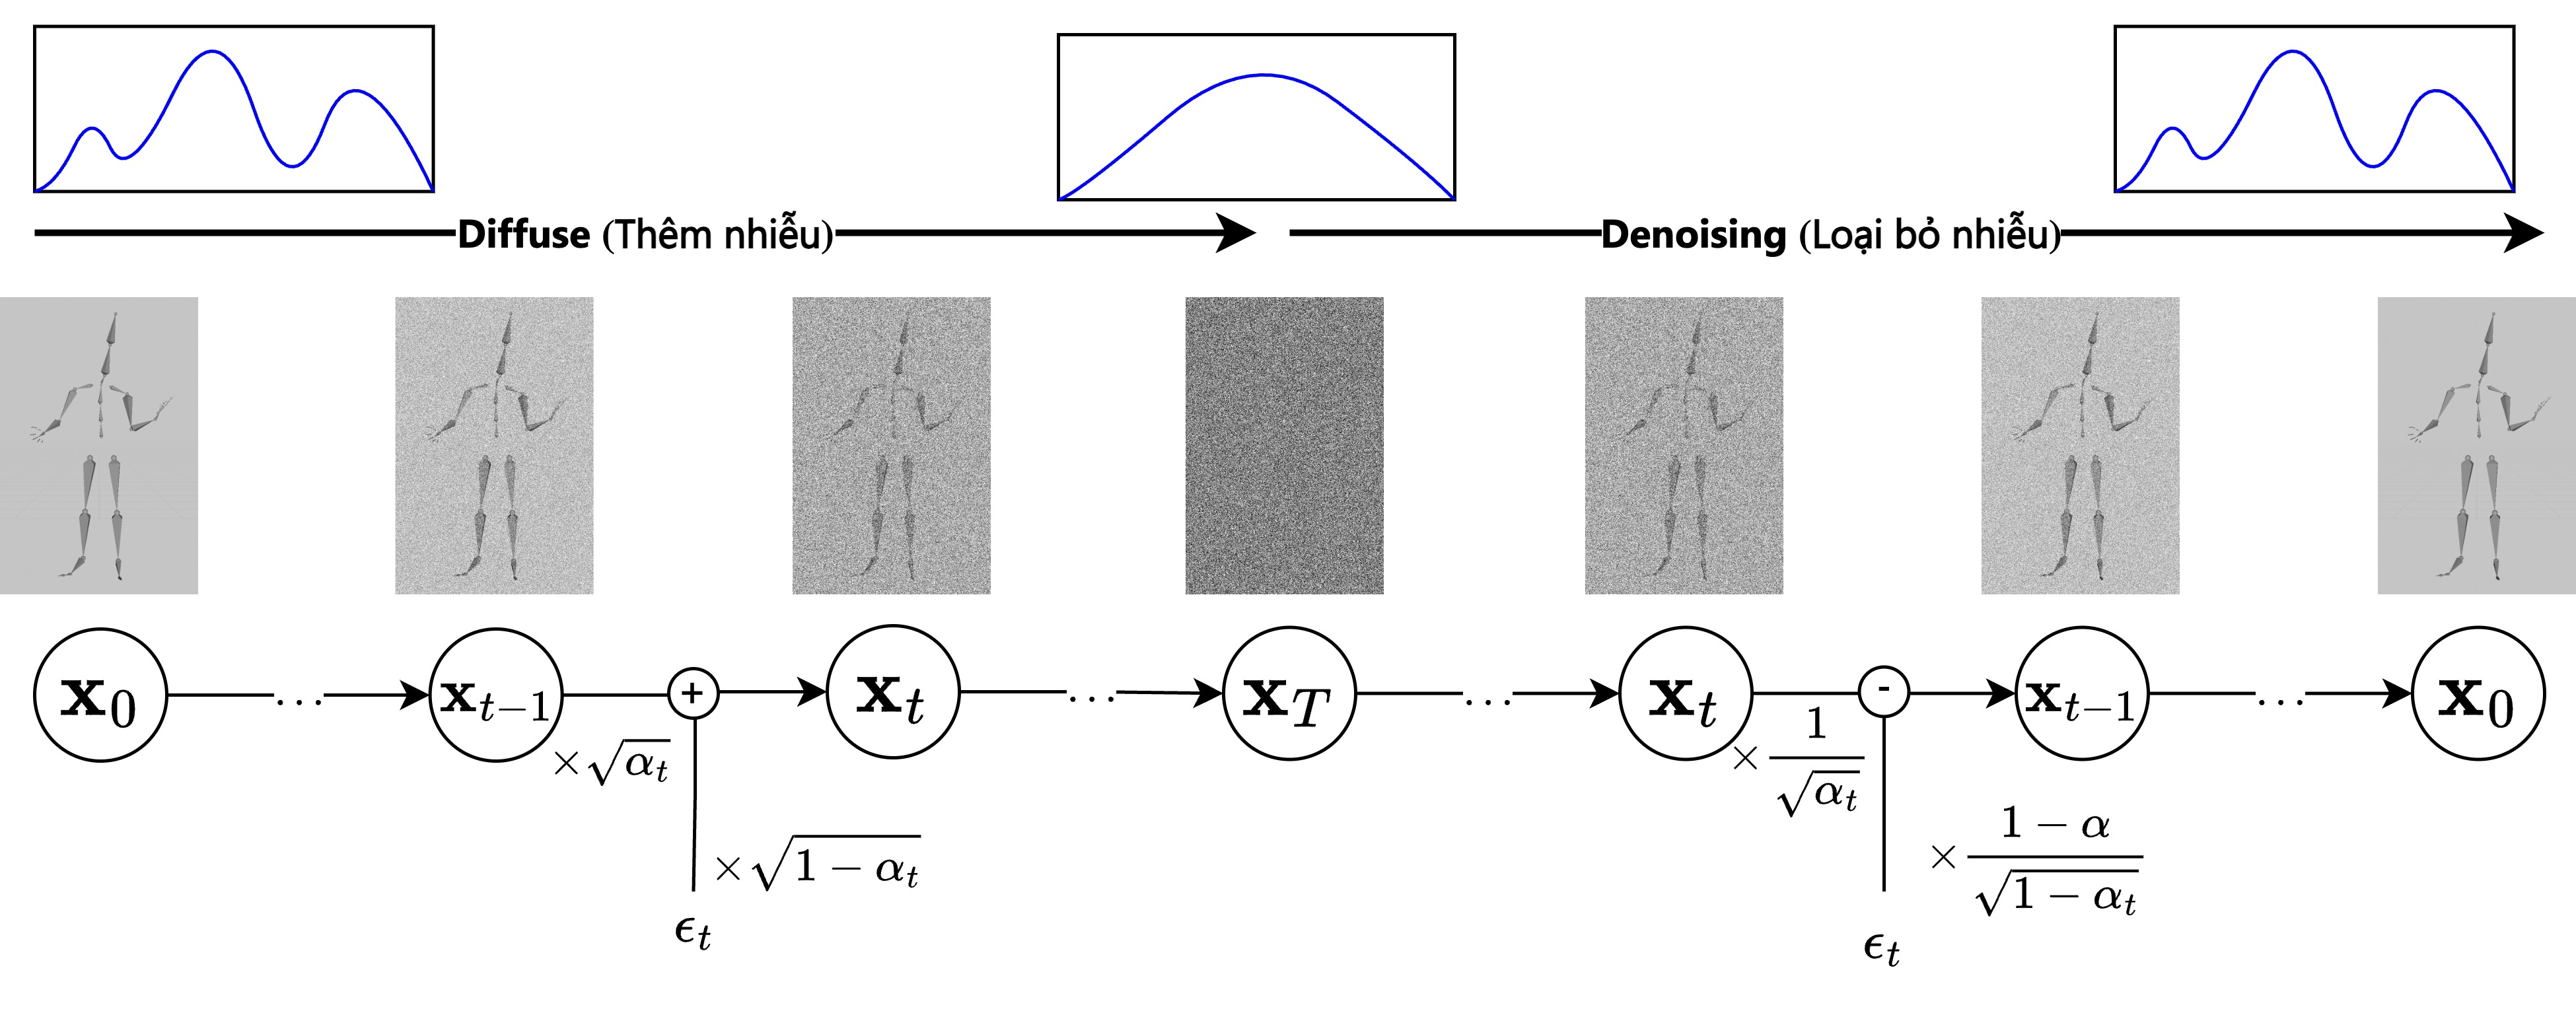
\includegraphics[width=\linewidth]{DiffuseAndDenoise.jpg}
	\caption{The \textbf{non-training} Diffusion and Denoising Process}
	\label{fig:DiffuseAndDenoise}
\end{figure}

In neural network methods like ResNet or InceptionNet, the goal is to learn the weight $\theta$ of a function $f_{\theta}(x)$ by minimizing a loss function $\mathcal{L}_\text{loss}$ between a label $y$ and its prediction $\hat{y}$. Once training is complete, the learned weight $\theta'$ can be used to predict a new sample $x'$ through $f_{\theta'}$ to obtain prediction $y'$.

Similarly to VAE, where the input matrix is encoded into a latent vector $z$ and then decoded back into a matrix of the original size, the diffusion model breaks the learning process into $T$ steps. At each step $t$, the forward diffusion process $q(\mathbf{x})$ from $1 \to T$ adds Gaussian noise $\epsilon_t \sim \mathcal{N}(\mathbf{0}, \mathbf{I})$, where $\mathbf{I}$ is the identity matrix of the standard Gaussian distribution with $\mathbb{E}[\epsilon] = 0$ and $\operatorname{Var}(\epsilon) = 1$.

The process of adding noise from left to right is called $q(\bx)$, while the denoising process from right to left is $p(\bx)$. Note that $\epsilon_t$ is randomly sampled at each step $t$, but once sampled, it is fixed. As illustrated in \autoref{fig:DiffuseAndDenoise}, if we add a noise $\epsilon_t$ during diffusion and subtract exactly the same noise during denoising, the result $\bx_0$ is \textbf{identical} to the original input.

However, during denoising, instead of subtracting the actual noise $\epsilon_t$, the model uses a function $f_{\theta}$ to \textbf{predict the added noise} during diffusion. Then, $\bx_T$ is iteratively denoised by subtracting the predicted noise to obtain $\hat{\bx}_{T-1}$, continuing until $\hat{\bx}_0$ is reached.

In the basic Diffusion model or Denoising Diffusion Probabilistic Models (DDPM \cite{ho2020denoising}), the denoising process goes from $T \to 1$, and the goal is to learn the weights $\theta$ of the noise prediction function $f_{\theta}$ (also denoted as $\epsilon_\theta$). After training, the learned weights $\theta'$ are used to predict the noise $\hat{\epsilon}$. Then, the noise is subtracted from the noisy image $\mathbf{x}_t$ to get $\mathbf{x}_{t-1}$, with additional noise $\mathbf{z} \sim \mathcal{N}(0, \mathbf{I})$ added to maintain gesture diversity. This process is repeated until reaching the final prediction $\hat{\bx}_0$.

\subsection{Forward Diffusion Process}

Given the input data $\mathbf{x}_0 \sim q(x)$ from the real dataset, at each step $t$, noise is added to $\mathbf{x}_{0}$ with the noise-to-signal ratio controlled by a factor $\beta$:

\begin{equation}
	\label{eq:addgaussian}
	\mathbf{x}_t = \sqrt{1 - \beta_t}\mathbf{x}_{t-1} + \sqrt{\beta_t} \boldsymbol{\epsilon}_{t-1}
\end{equation}

The forward process runs from $1 \to T$, with $\beta_t \in (0, 1)$ for each $t$.

Since a function of the form $f(x) = ax + b\epsilon$, with $\epsilon \sim \mathcal{N}(0, \mathbf{I})$, implies $f(x) \sim \mathcal{N}(ax, b^2)$, the forward process can be reformulated as:

\begin{equation}
	\label{eq:forward_diffusion_process}
	\begin{aligned}
		q(\mathbf{x}_t \vert \mathbf{x}_{t-1}) &= \mathcal{N}(\mathbf{x}_t; \sqrt{1 - \beta_t} \mathbf{x}_{t-1}, \beta_t\mathbf{I}) \quad \\
		q(\mathbf{x}_{1:T} \vert \mathbf{x}_0) &= \prod^T_{t=1} q(\mathbf{x}_t \vert \mathbf{x}_{t-1})
	\end{aligned}
\end{equation}

Here, $\sqrt{1 - \beta_t}$ gradually decreases the contribution of $\mathbf{x}_t$, while $\beta_t$ increases the noise component. Typically, $\beta_1 < \beta_2 < \dots < \beta_T$. As $T \to \infty$, $\mathbf{x}_T$ approaches a pure Gaussian distribution: $q(\mathbf{x}_T) = \mathcal{N}(0, \mathbf{I})$ \cite{weng2021diffusion}.

\begin{figure}[h]
	\centering
	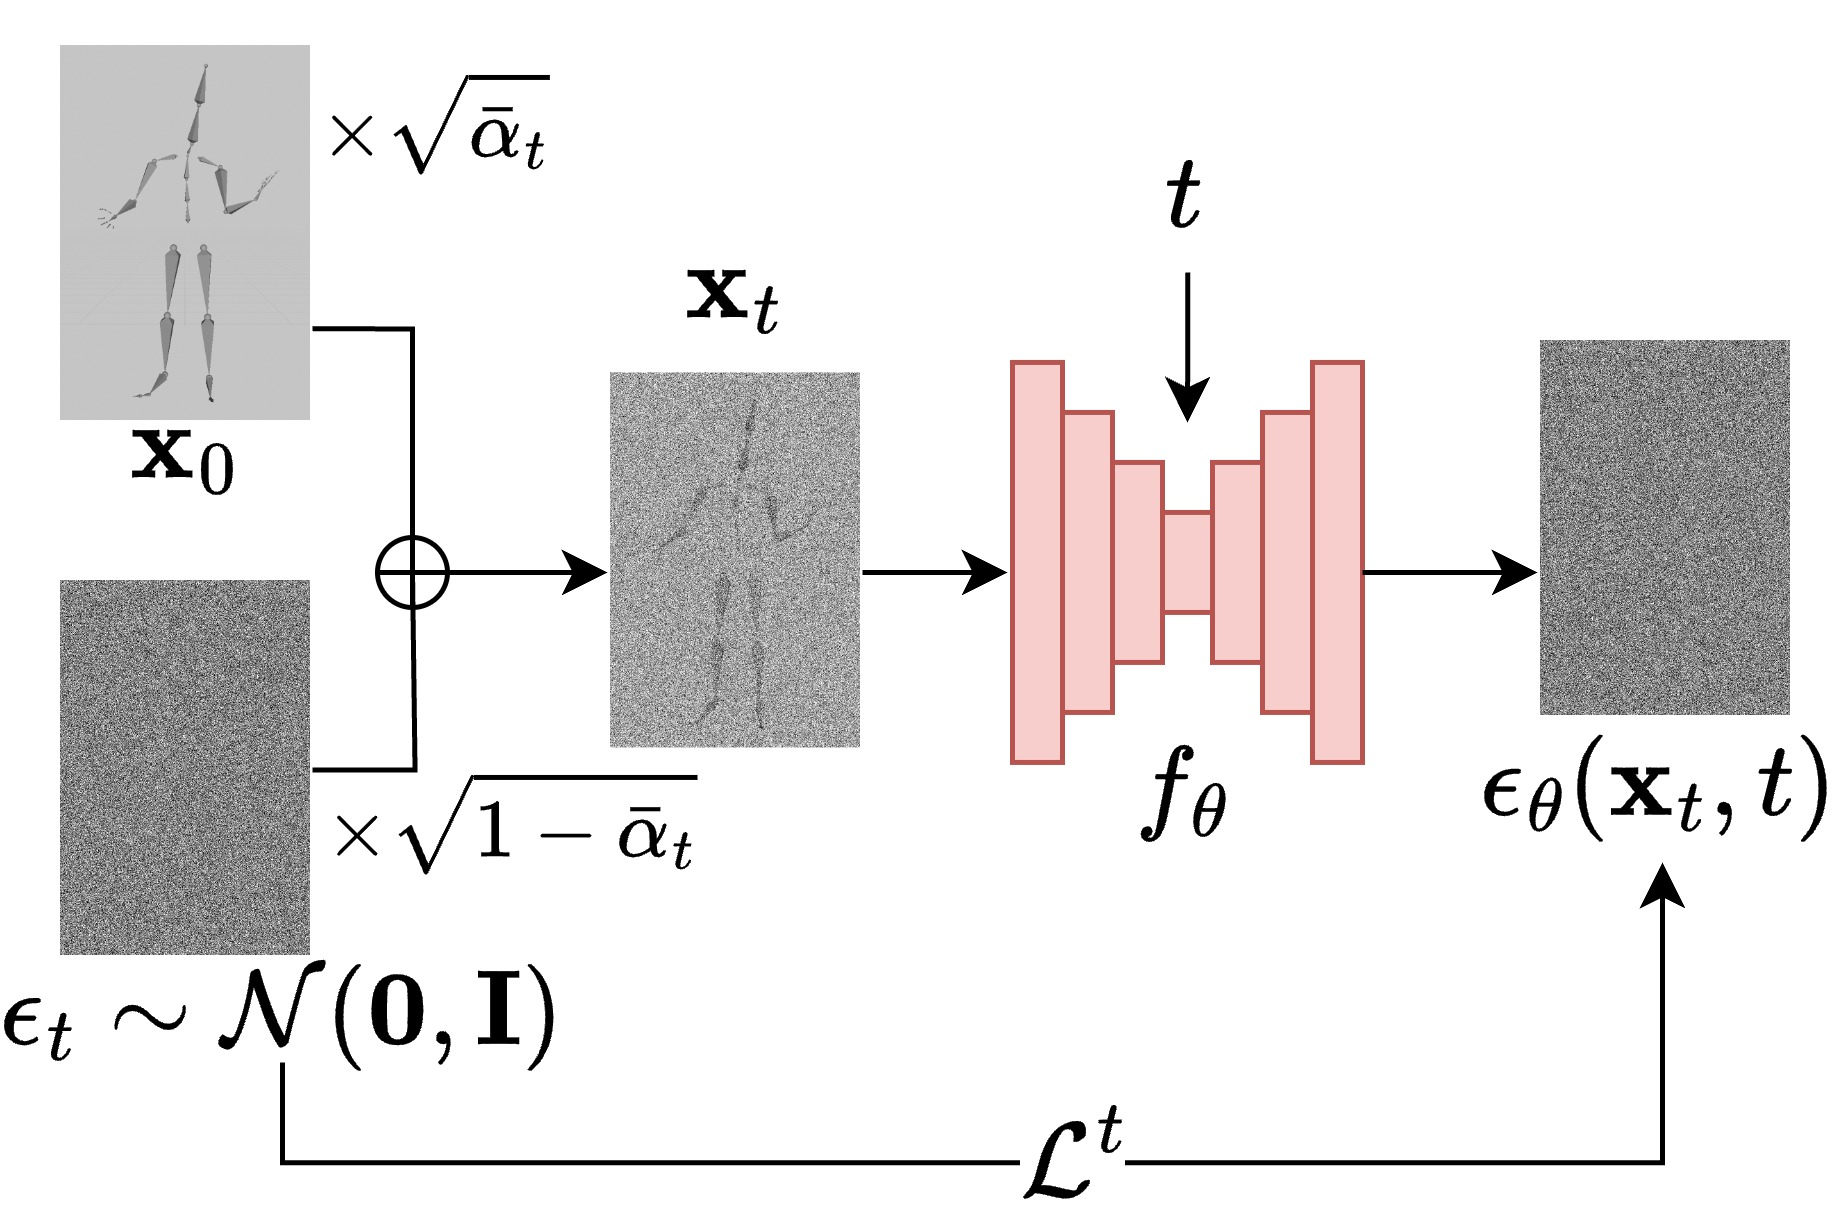
\includegraphics[height=160pt]{AlgorithmForwardDiffusion}
	\caption{Noise addition during training}
	\label{fig:AlgorithmForwardDiffusion}
\end{figure}

Since $\boldsymbol{\epsilon}_{t-1}, \boldsymbol{\epsilon}_{t-2}, \dots \sim \mathcal{N}(\mathbf{0}, \mathbf{I})$ and fixed for each $t$, $\bx_t$ can be computed directly from $\bx_0$. Define $\alpha_t = 1 - \beta_t$ and $\bar{\alpha}_t = \prod_{i=1}^t \alpha_i$, then \autoref{eq:addgaussian} becomes:

%\begin{equation}
%\begin{aligned}
%	\boldsymbol{x}_t &= \sqrt{\bar{\alpha}_t} \boldsymbol{x}_0 + \sqrt{1 - \bar{\alpha}_t} \boldsymbol{\epsilon}_0 \\
%	&\sim \mathcal{N}\left(\boldsymbol{x}_t; \sqrt{\bar{\alpha}_t} \boldsymbol{x}_0, \left(1 - \bar{\alpha}_t\right) \textbf{I}\right)
%\end{aligned}
%\label{eq:tracexzero}
%\end{equation}

\begin{equation}
	\begin{aligned}
		\boldsymbol{x}_t &= \sqrt{\alpha_t}\boldsymbol{x}_{t-1} + \sqrt{1 - \alpha_t}\boldsymbol{\epsilon}_{t-1} \\
		&= \sqrt{\alpha_t}\left(\sqrt{\alpha_{t-1}}\boldsymbol{x}_{t-2} + \sqrt{1 - \alpha_{t-1}}\boldsymbol{\epsilon}_{t-2}\right) + \sqrt{1 - \alpha_t}\boldsymbol{\epsilon}_{t-1} \\
		&= \sqrt{\alpha_t\alpha_{t-1}}\boldsymbol{x}_{t-2} + \sqrt{\alpha_t(1 - \alpha_{t-1})}\boldsymbol{\epsilon}_{t-2} + \sqrt{1 - \alpha_t}\boldsymbol{\epsilon}_{t-1} \\
		&= \sqrt{\alpha_t\alpha_{t-1}}\boldsymbol{x}_{t-2} + \sqrt{\alpha_t(1 - \alpha_{t-1}) + (1 - \alpha_t)}\boldsymbol{\epsilon}_{t-2} \\
		&= \sqrt{\alpha_t\alpha_{t-1}}\boldsymbol{x}_{t-2} + \sqrt{1 - \alpha_t\alpha_{t-1}}\boldsymbol{\epsilon}_{t-2} \\
		&= \ldots \\
		&= \sqrt{\prod_{i=1}^t \alpha_i} \boldsymbol{x}_0 + \sqrt{1 - \prod_{i=1}^t \alpha_i} \boldsymbol{\epsilon}_0 \\
		&= \sqrt{\bar{\alpha}_t} \boldsymbol{x}_0 + \sqrt{1 - \bar{\alpha}_t} \boldsymbol{\epsilon}_0 \\
		&\sim \mathcal{N}\left(\boldsymbol{x}_t; \sqrt{\bar{\alpha}_t} \boldsymbol{x}_0, \left(1 - \bar{\alpha}_t\right) \textbf{I}\right)
	\end{aligned}
	\label{eq:tracexzero}
\end{equation}

The evolution of $\sqrt{\alpha}$ and $\sqrt{1 - \alpha}$ over diffusion steps is shown in Appendix \autoref{appendix:Appendix1}.

\subsection{Denoising Process}
\label{subsection:denoising_process}

\begin{figure}[h]
	\centering
	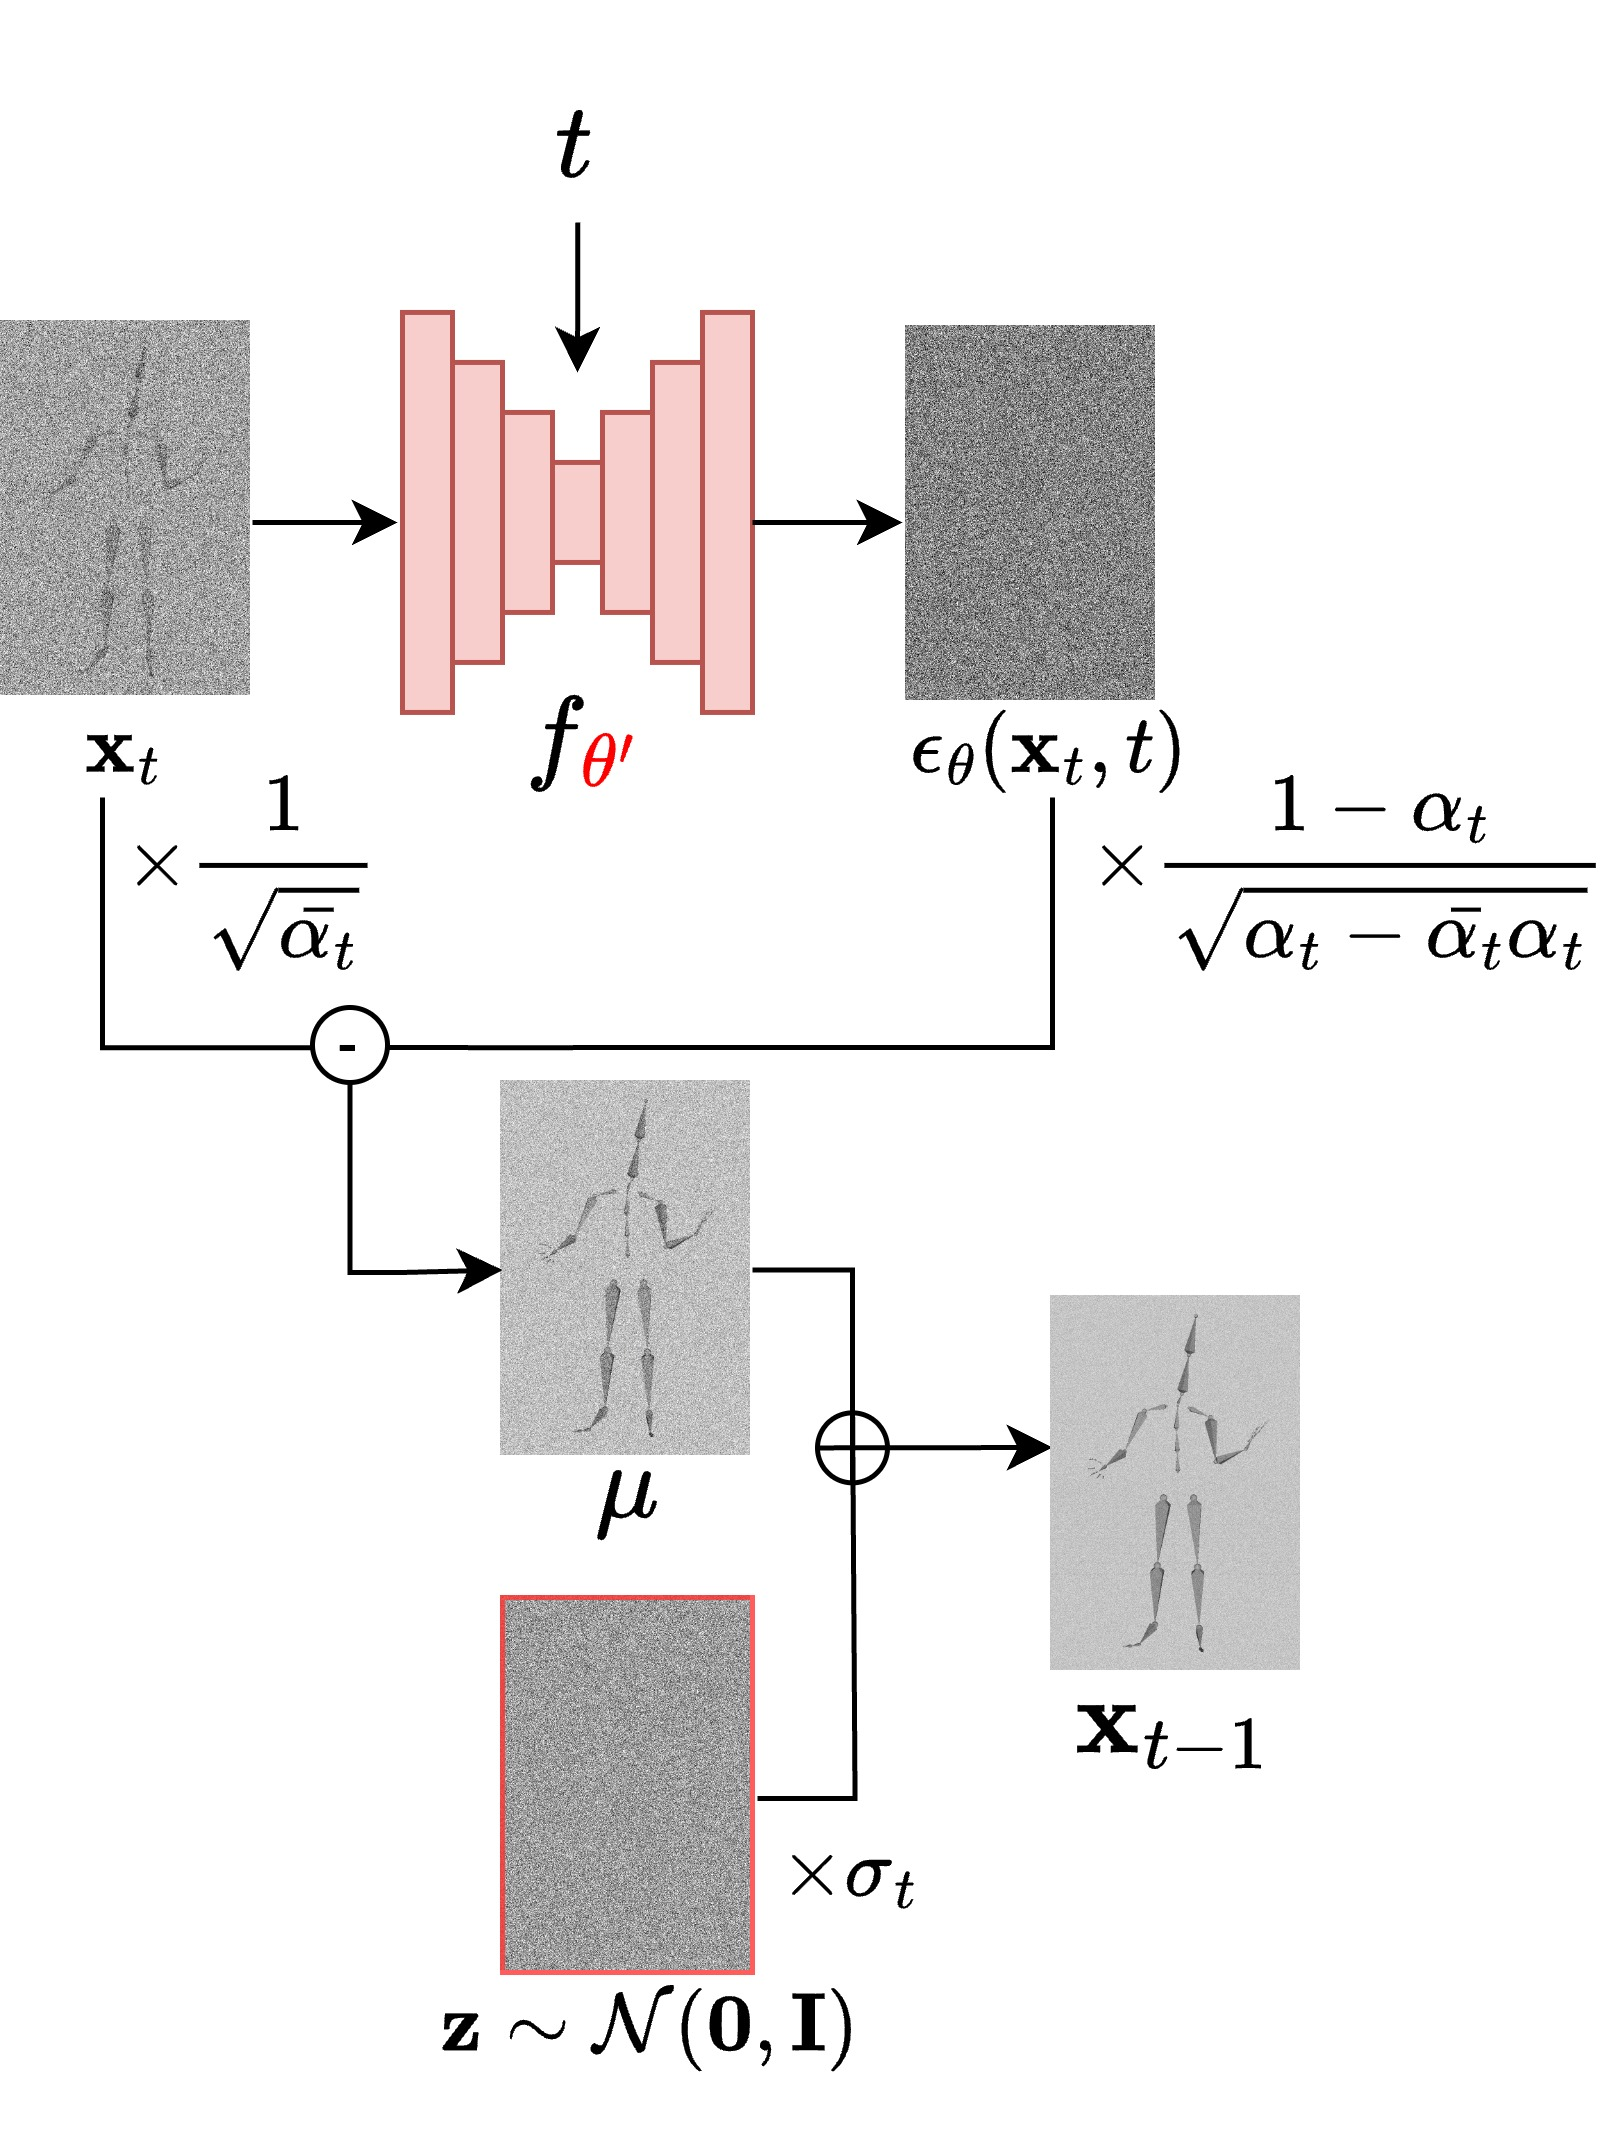
\includegraphics[height=280pt]{AlgorithmSamplingDiffusion}
	\caption{Denoising during inference}
	\label{fig:AlgorithmSamplingDiffusion}
	\vspace{-5pt}
\end{figure}

The denoising process $p_\theta(\mathbf{x}_{t-1} \vert \mathbf{x}_t)$ starts from $\bx_T \sim \mathcal{N}(\mathbf{0}, \mathbf{I})$. A neural network $f_{\theta}(\bx_t, t)$ is used to predict the noise $\hat{\epsilon}_t = f_{\theta}(\bx_t, t)$.

The denoising distribution has mean and variance:

\begin{equation}
	\label{eq:denoising_process}
	\begin{aligned}
		p_\theta(\mathbf{x}_{0:T})
		&= p(\mathbf{x}_T) \prod^T_{t=1} p_\theta(\mathbf{x}_{t-1} \vert \mathbf{x}_t) \\
		p_\theta(\mathbf{x}_{t-1} \vert \mathbf{x}_t) &= \mathcal{N}(\mathbf{x}_{t-1};  \boldsymbol{\mu}_\theta(\mathbf{x}_t, t), \boldsymbol{\Sigma}_\theta(\mathbf{x}_t, t))
	\end{aligned}
\end{equation}

where $\boldsymbol{\mu}_\theta(\mathbf{x}_t, t) = {\frac{1}{\sqrt{\alpha_t}} \left( \mathbf{x}_t - \frac{1 - \alpha_t}{\sqrt{1 - \bar{\alpha}_t}}  f_\theta(\mathbf{x}_t, t) \right)}$.

\subsection{Training Process in the Basic Diffusion Model}

\begin{figure}[h]
	\centering
	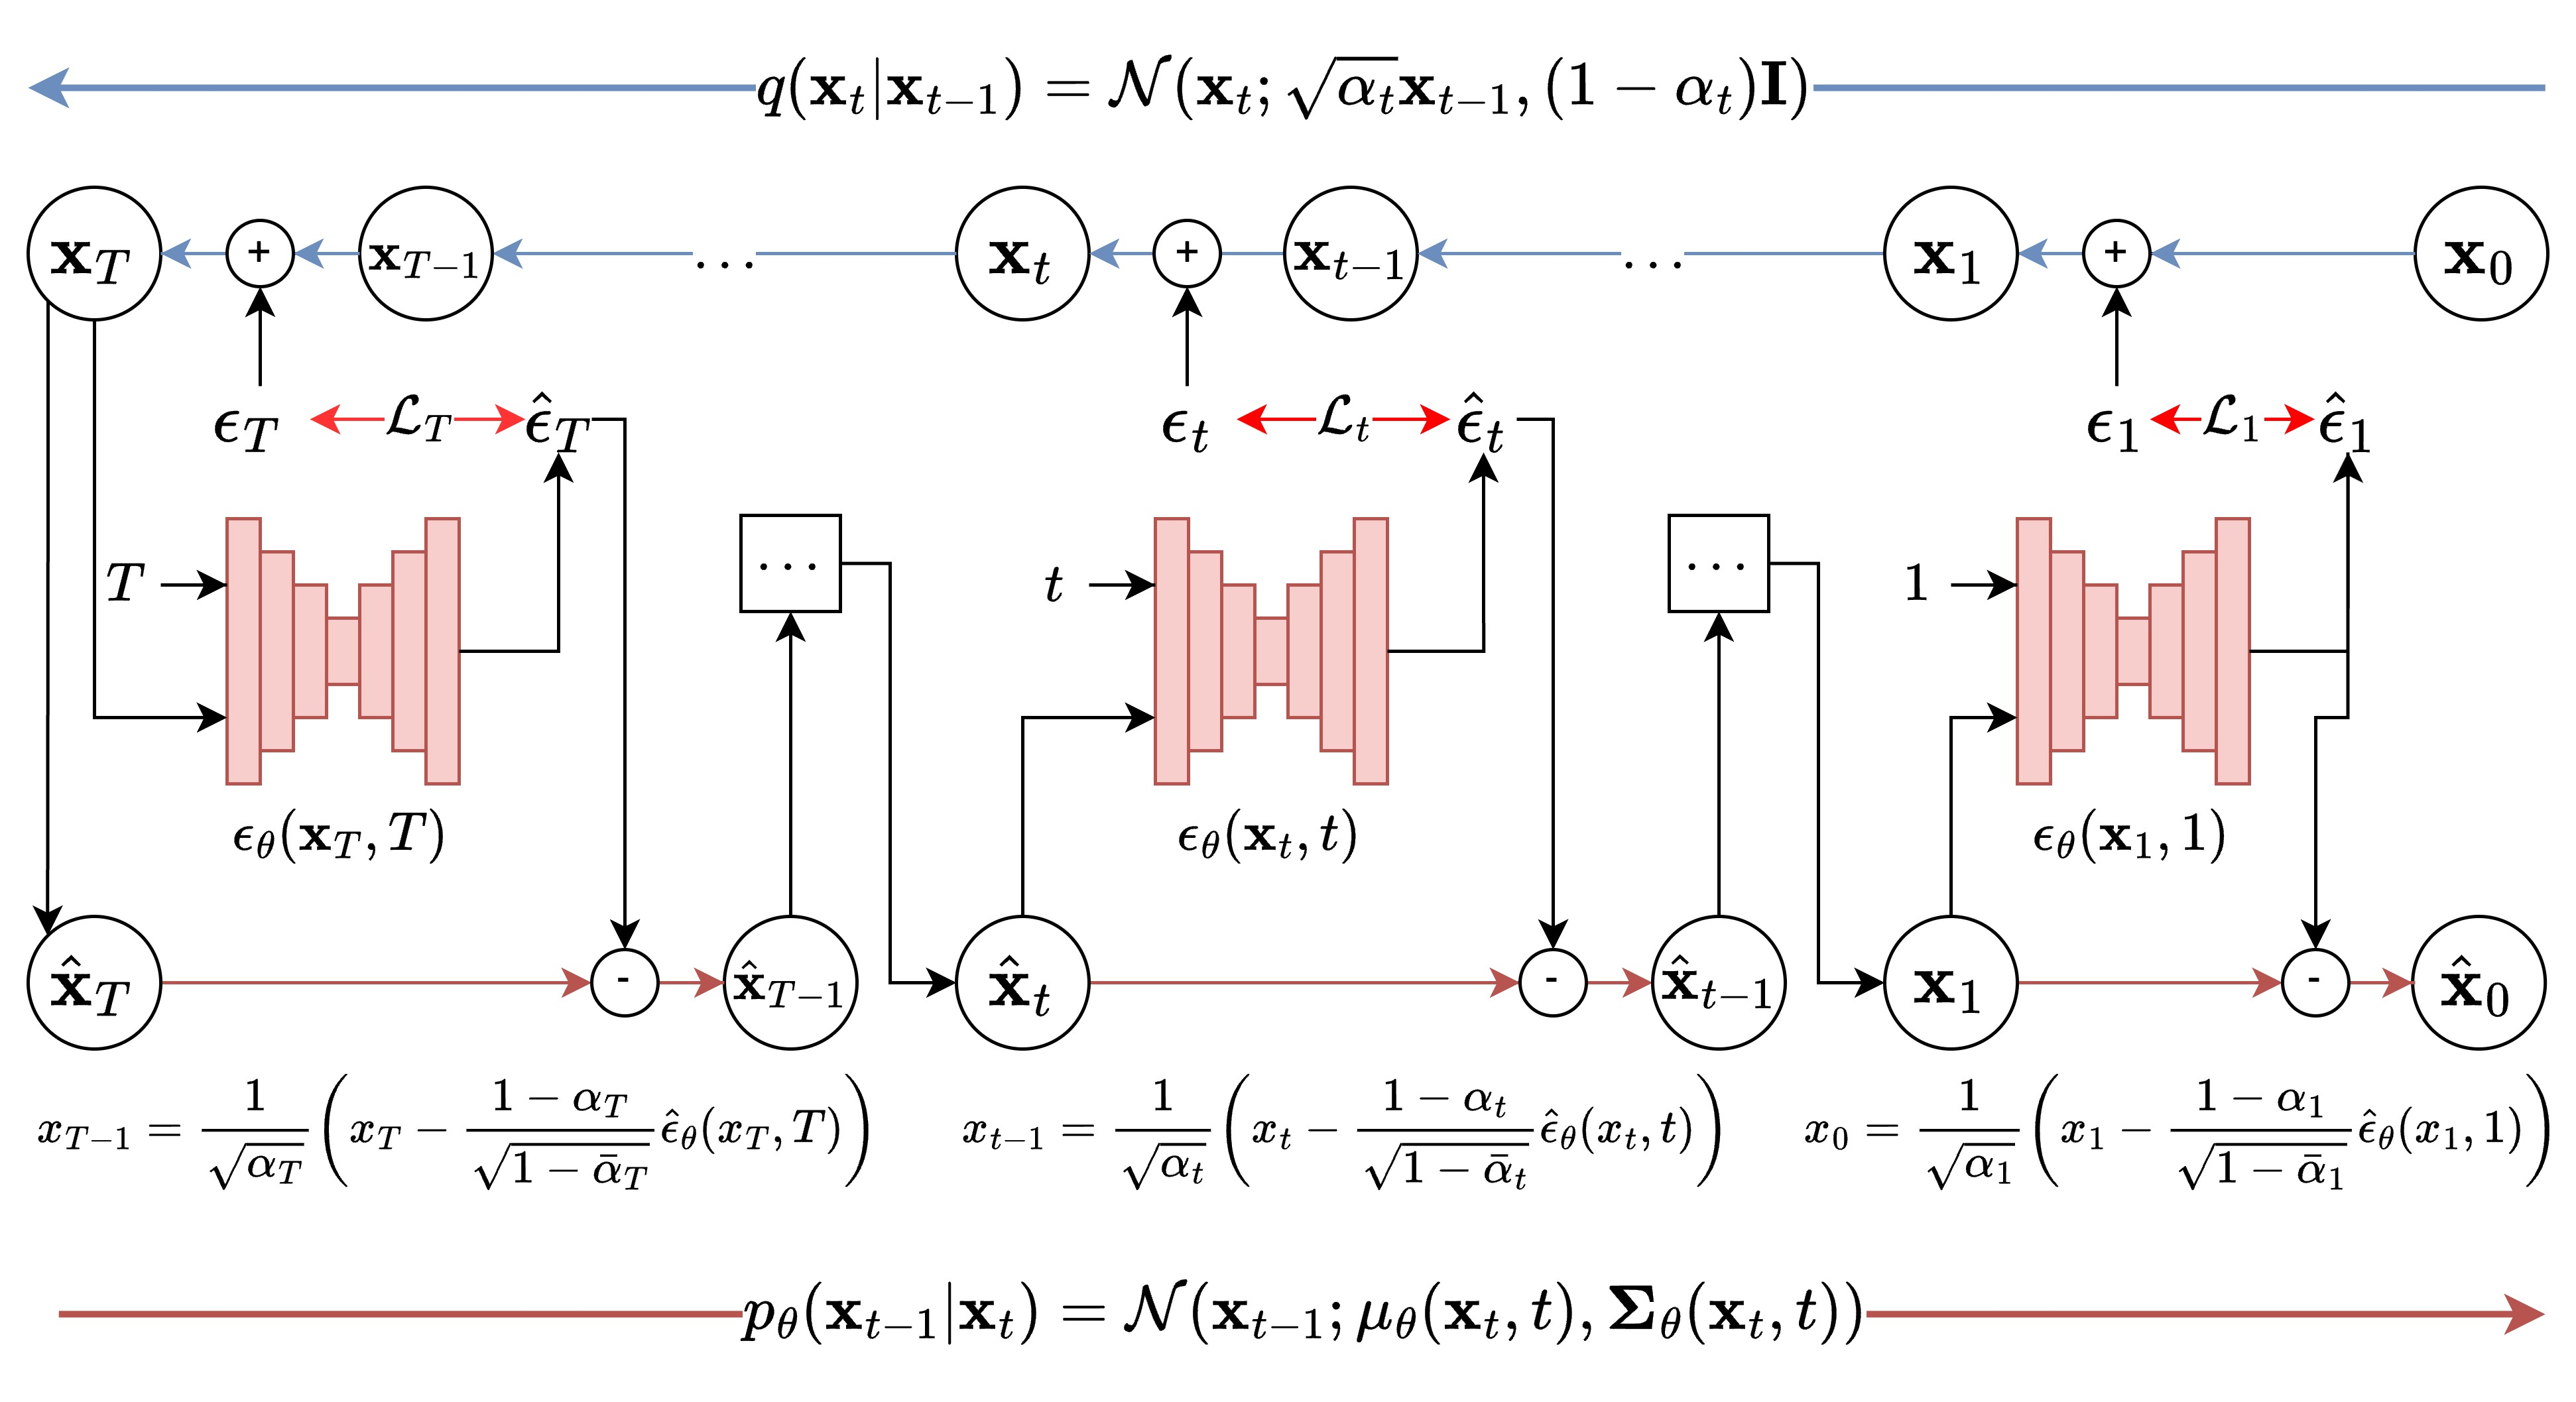
\includegraphics[width=\linewidth]{DDPMTraining}
	\caption{Basic diffusion model}
	\label{fig:basic_diffusion}
	\vspace{-5pt}
\end{figure}

The diffusion model learns the parameters $\theta$ of the noise prediction function $f_{\theta}(\bx_t, t)$ (or $\epsilon_\theta$). During denoising, we minimize the loss between the predicted noise $\boldsymbol{\epsilon}_\theta(\bx_t, t)$ and actual noise $\boldsymbol{\epsilon}_t$ at each step $t$:

\begin{equation}
	\label{eq:diffusion_loss}
	\begin{aligned}
		\mathcal{L}^t
		&= \mathbb{E}_{t \sim [1, T], \bx_0, \boldsymbol{\epsilon}_t} \left[\|\boldsymbol{\epsilon}_t - \boldsymbol{\epsilon}_\theta(\bx_t, t)\|^2 \right] \\
		&= \mathbb{E}_{t \sim [1, T], \bx_0, \boldsymbol{\epsilon}_t} \left[\|\boldsymbol{\epsilon}_t - \boldsymbol{\epsilon}_\theta(\sqrt{\bar{\alpha}_t}\bx_0 + \sqrt{1 - \bar{\alpha}_t}\boldsymbol{\epsilon}_t, t)\|^2 \right]
	\end{aligned}
\end{equation}

The total loss is $\mathcal{L} = \sum_{t=1}^T \mathcal{L}^t$.

Here, $f_{\theta}(x_t, t)$ or $\epsilon_\theta$ is a U-Net model used to encode and decode the data for noise prediction. The computation process is illustrated in \autoref{fig:basic_diffusion}.

\begin{algorithm}[h]
	\setlength{\baselineskip}{10pt}
	\begin{enumerate}
		\vspace{5pt}
		\item Precompute $\sqrt{\alpha_t}$, $\sqrt{1 - \alpha_t}$, and $\sqrt{\bar{\alpha}_t}$ for $t = 1 \rightarrow T$. Define noise schedule $\{\alpha_t \in (0, 1)\}_{t=1}^T$ with $\alpha_1 < \alpha_2 < \dots < \alpha_T$.
		
		\item Sample label $\bx_0$ from the normalized data distribution.
		
		\item Generate random noise $\boldsymbol{\epsilon}_t$ for each step $t = 1 \rightarrow T$, where $\boldsymbol{\epsilon}_t \sim \mathcal{N}(\mathbf{0}, \mathbf{I})$.
		
		\item Apply forward diffusion to get $\bx_t$:
		$$
		\bx_t = \sqrt{\bar{\alpha}_t} \bx_0 + \sqrt{1 - \bar{\alpha}_t} \boldsymbol{\epsilon}_t
		$$
		
		\item Randomly select $t \in [1, T]$.
		
		\item Feed $\bx_t$ and $t$ into the model to predict noise: $\hat{\boldsymbol{\epsilon}} = \boldsymbol{\epsilon}_\theta(\bx_t, t)$.
		
		\item Compute the gradient:
		$$
		\grad_{\theta_t} \left\| \boldsymbol{\epsilon}_t - \boldsymbol{\epsilon}_\theta(\bx_t, t) \right\|^2
		$$
		
		And loss:
		$$
		\mathcal{L}^t = \mathbb{E}_{t, \bx_0, \boldsymbol{\epsilon}_t} \left[ \|\boldsymbol{\epsilon}_t - \boldsymbol{\epsilon}_\theta(\sqrt{\bar{\alpha}_t} \bx_0 + \sqrt{1 - \bar{\alpha}_t} \boldsymbol{\epsilon}_t, t)\|^2 \right]
		$$
		
		\item Repeat step 6 until convergence to obtain optimal weights $\theta'$.
	\end{enumerate}
	\caption{DDPM Training Algorithm}
	\label{alg:TrainingDDPM}
\end{algorithm}

\subsection{Basic Sampling Process in Diffusion Models}

\begin{figure*}
	\centering
	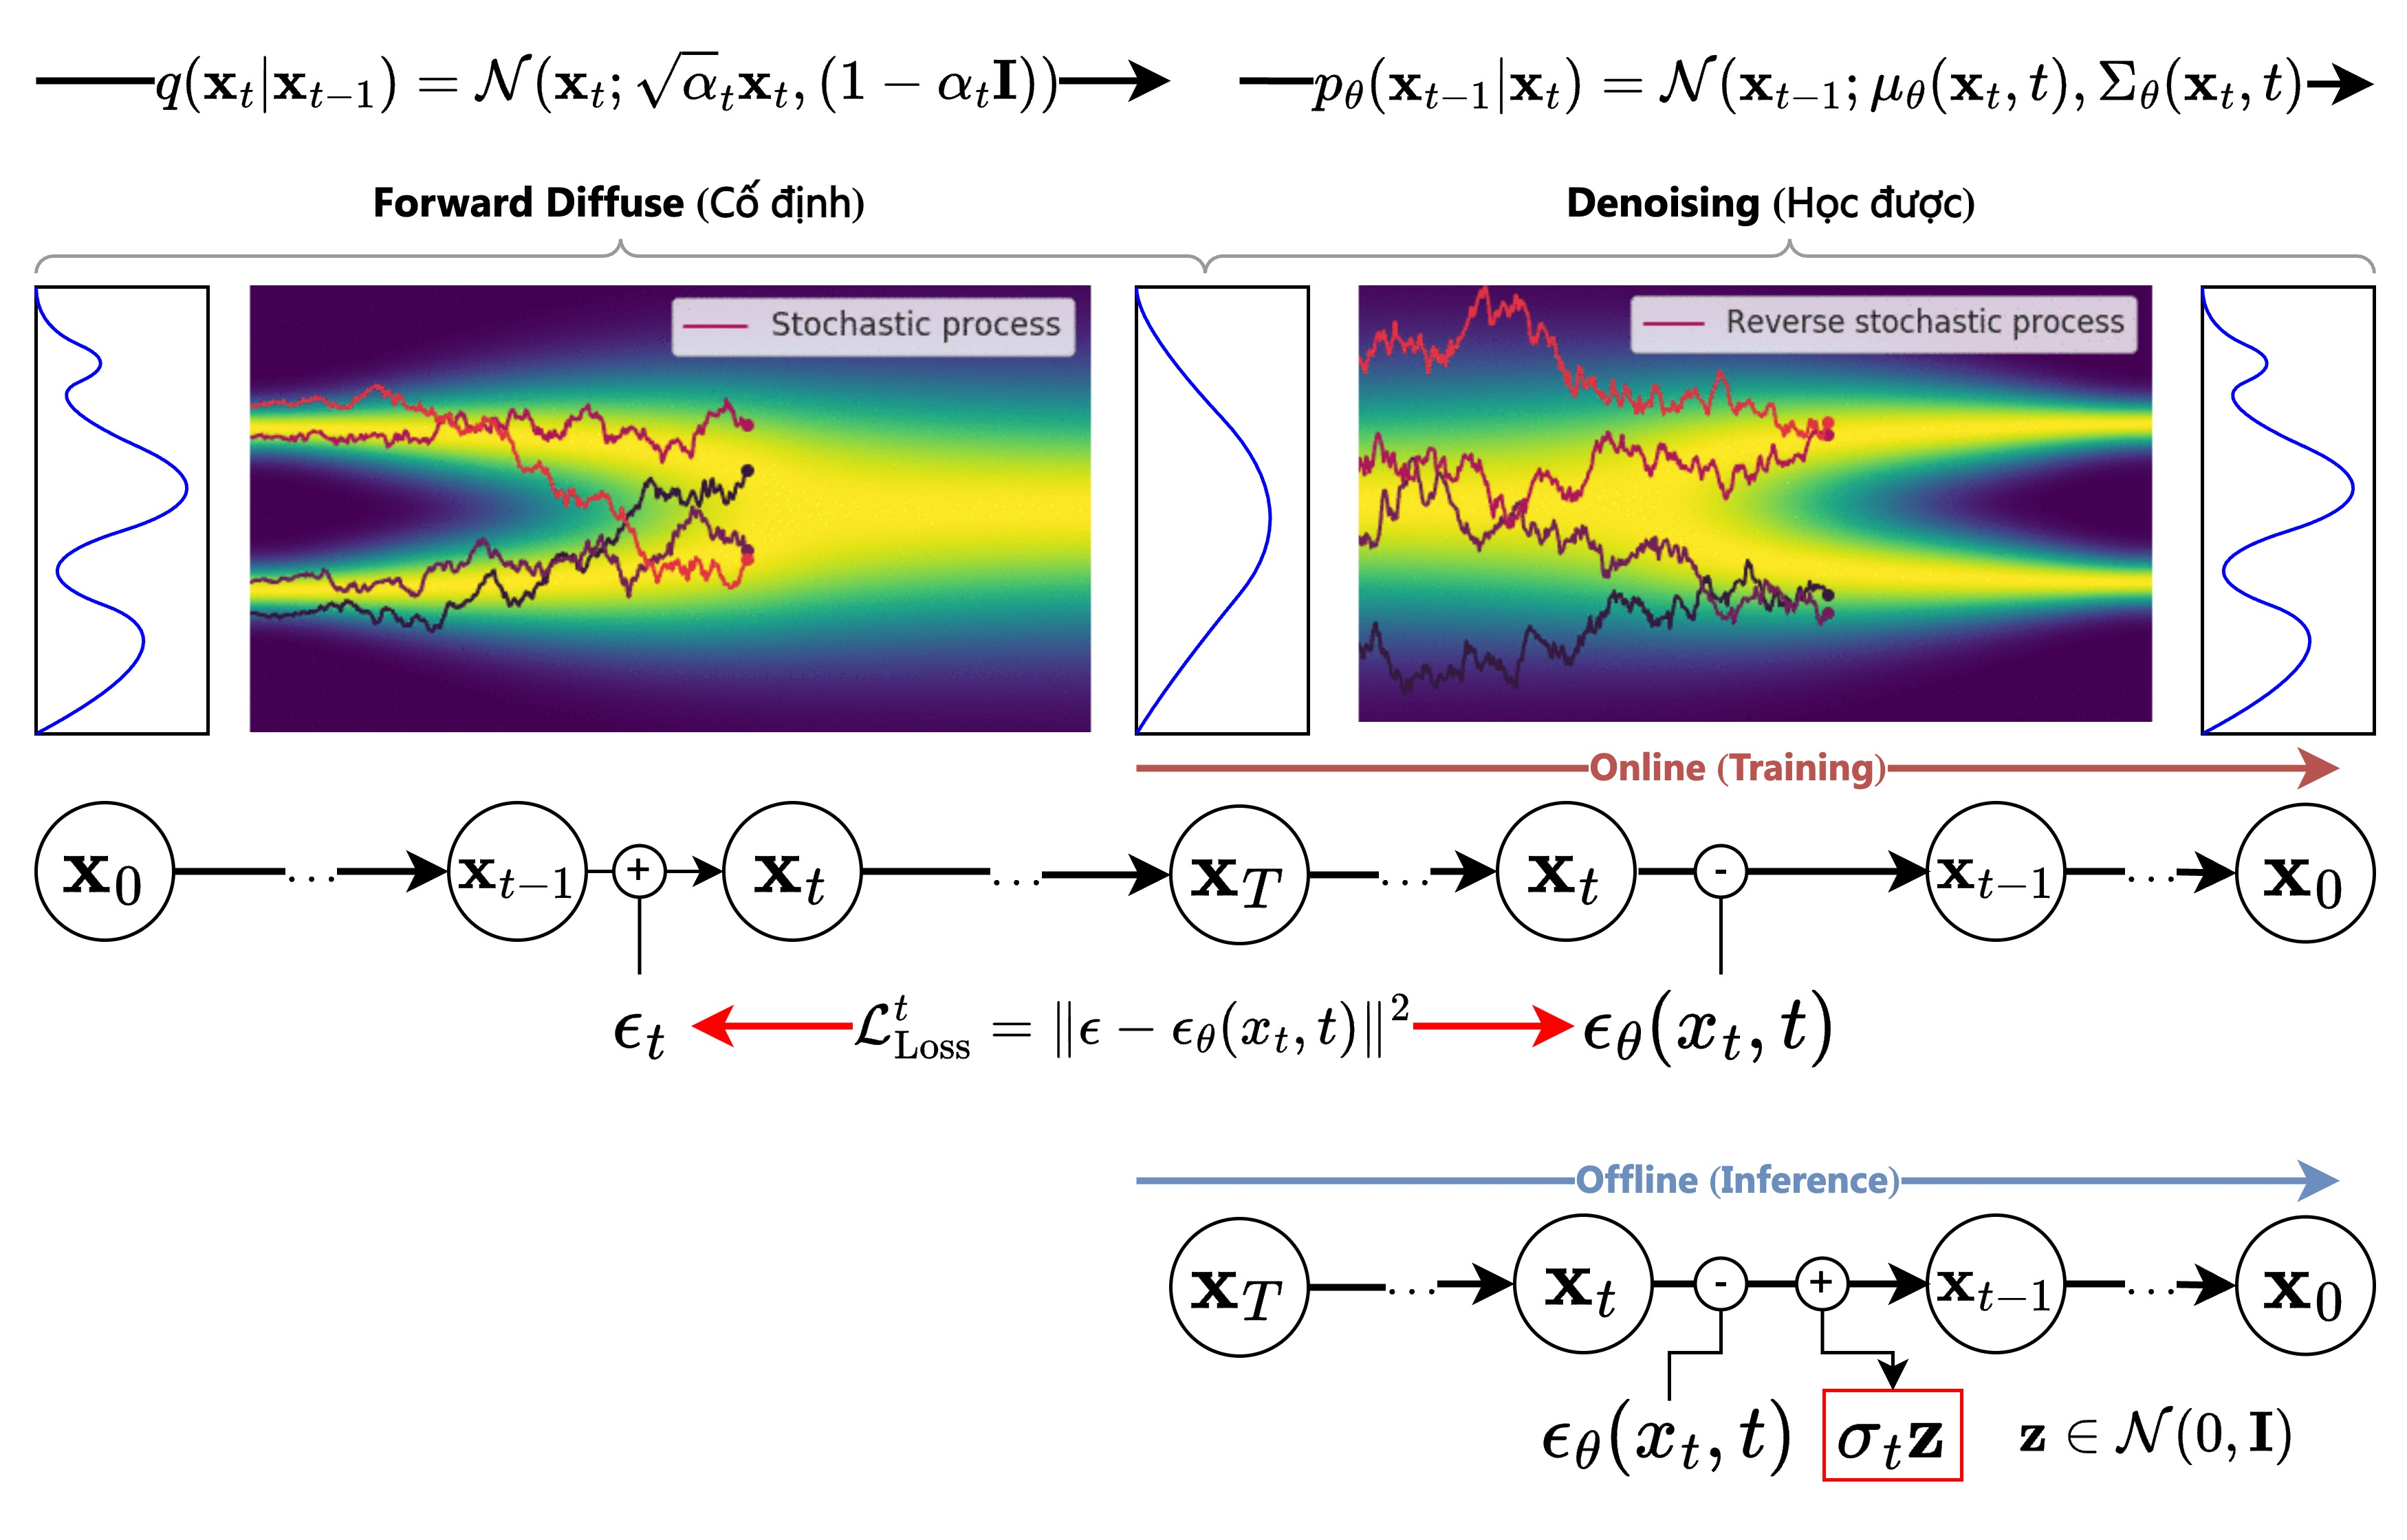
\includegraphics[width=\linewidth]{TrainingAndSamplingStandard}
	\caption{Training and Sampling process in a standard Diffusion model}
	\label{fig:GaussianDrift}
\end{figure*}

After obtaining the weights $\theta'$, the denoising function is used to denoise from noise $\bx_T \sim \mathcal{N} (\mathbf{0}, \mathbf{I})$.  
The transformation from pure noise $\bx_{T}$ to the prediction $\hat{\bx_0}$ is as follows:

\begin{equation}
	\label{eq:adddenoising}
	\bx_{t-1} = \frac{1}{\sqrt{\alpha_t}} \left( \bx_t - \frac{1- \alpha_t}{\sqrt{1 - \bar{\alpha}_t}} f_{\theta'}(\bx_t, t) \right) + \sqrt{1 - \alpha_t} \tilde{\epsilon}_t
\end{equation}

Note that $\epsilon_t$ is fixed and randomly generated noise created before the training process, and reused during the forward diffusion process \autoref{subsection:denoising_process} in formula \autoref{eq:addgaussian}. As shown in \autoref{fig:GaussianDrift}, the error $\epsilon_t$ corresponds to the noise at each step $t$, and the loss function $\mathcal{L}^{t}$ is computed per time step $t$.

Following the training process, the DDPM sampling algorithm begins from pure noise, i.e., $\mathbf{x}_T \sim \mathcal{N}(0, \mathbf{I})$, where the initial data is entirely noise. The values $\sqrt{\alpha_t}$, $\sqrt{1 - \alpha_t}$, and $\sqrt{\bar{\alpha}_t}$, obtained from the training phase, are used during sampling to reconstruct the original data $\mathbf{x}_0$. The next step is to compute the noise adjustment coefficient $\sigma_t$, based on the noise schedule $\alpha_t$ defined during training. These values influence the amount of noise added in the reverse sampling process.

The sampling process (\autoref{alg:samplingddpm}) proceeds from step $T$ down to $1$, and at each step, a random noise $\mathbf{z} \sim \mathcal{N}(0, \mathbf{I})$ is generated and added to the predicted result. At each step $t$, the model predicts the noise $\boldsymbol{\epsilon}_{\theta'}$ based on the noisy data $\mathbf{x}_t$ and time step $t$, then uses this prediction to compute the value $\mu$, an estimate of $\mathbf{x}_0$. Finally, a noise term $\sigma_t \mathbf{z}$ is added to $\mu$ to obtain $\hat{\mathbf{x}}_{t-1}$, the noisy data at step $t-1$. This process continues until $t = 1$, at which point $\hat{\mathbf{x}}_0$ — the final prediction of the original data — is obtained through denoising.

\begin{algorithm}[h]
	\caption{Sampling algorithm in DDPM}
	\label{alg:samplingddpm}
	\setlength{\baselineskip}{10pt}
	\begin{enumerate}
		\item Start with noise: $\mathbf{x}_T \sim \mathcal{N}(0, \mathbf{I})$.
		
		\item Retrieve values $\sqrt{\alpha_t}$, $\sqrt{1 - \alpha_t}$, and $\sqrt{\bar{\alpha}_t}$ from the training process.
		
		\item Compute the noise adjustment coefficient $\sigma_t$ from $\alpha_t$ at each step $t: 1 \rightarrow T$:
		\[
		\sigma_t = \sqrt{\frac{1 - \bar{\alpha}_{t-1}}{1 - \bar{\alpha}_t} (1 - \alpha_t)}
		\]
		
		\item For each $t$, iterate \textbf{sequentially} from $[T, \dots, 1]$.
		
		\item Generate random noise $\mathbf{z} \sim \mathcal{N}(0, \mathbf{I})$.
		
		\item Feed $\mathbf{x}_t$ into the model to infer noise: $\boldsymbol{\epsilon}_{\theta'} = \boldsymbol{\epsilon}_{\theta'}(\mathbf{x}_t, t)$.
		
		\item Use the predicted noise to subtract from $\mathbf{x}_t$ at step $t$:
		\[
		\mu = \frac{1}{\sqrt{\alpha_t}} \left( \mathbf{x}_t - \frac{1 - \alpha_t}{\sqrt{1 - \bar{\alpha}_t}} \boldsymbol{\epsilon}_{\theta'}(\mathbf{x}_t, t) \right)
		\]
		
		\item Add noise: $\hat{\mathbf{x}}_{t-1} = \mu + \sigma_t \mathbf{z}$.
		
		\item When $t = 1$, obtain $\hat{\mathbf{x}}_0$ from the denoising process.
	\end{enumerate}
\end{algorithm}

The most important aspect of the denoising sampling process is to add a noise term $\mathbf{z} \in \mathcal{N}(0, \mathbf{I})$, with $\mathbf{z}$ sequentially added at each step $t$ using the scaling factor $\sigma_t$. The goal of noise $\epsilon$ is to shape the marginal noise distribution so that model $f_\theta$ (or $\epsilon_{\theta}$) can learn to denoise, whereas $\mathbf{z}$ is used to increase diversity in generation and improve stability during sampling. The decay of $\sigma_t$ is detailed in Appendix \autoref{appendix:Appendix1:NoiseScale}.

\subsection{Improved Diffusion Model with $\bx_0$ Prediction Instead of $\epsilon_t$}
\label{subsec:X0Objective}

Based on \autoref{eq:tracexzero}, it is clear that given $\bx_t$, we can infer $\bx_0$. Conversely, given $\bx_0$, we can explicitly infer $\bx_t$ for any $t$ by adding the noise $\epsilon_t$ from the forward diffusion process.

From this observation, the authors in \cite{nichol2021improved} proposed an improvement to DDPM: instead of using the neural network $f_{\theta}(\bx_t, t)$ to predict $\epsilon_t$ as in \autoref{fig:basic_diffusion}, the function $f_{\theta}(\bx_t, t)$ is repurposed to directly predict $\bx_0$, after which noise is added using \autoref{eq:tracexzero}.

\begin{figure}[h]
	\captionsetup{skip=2pt}
	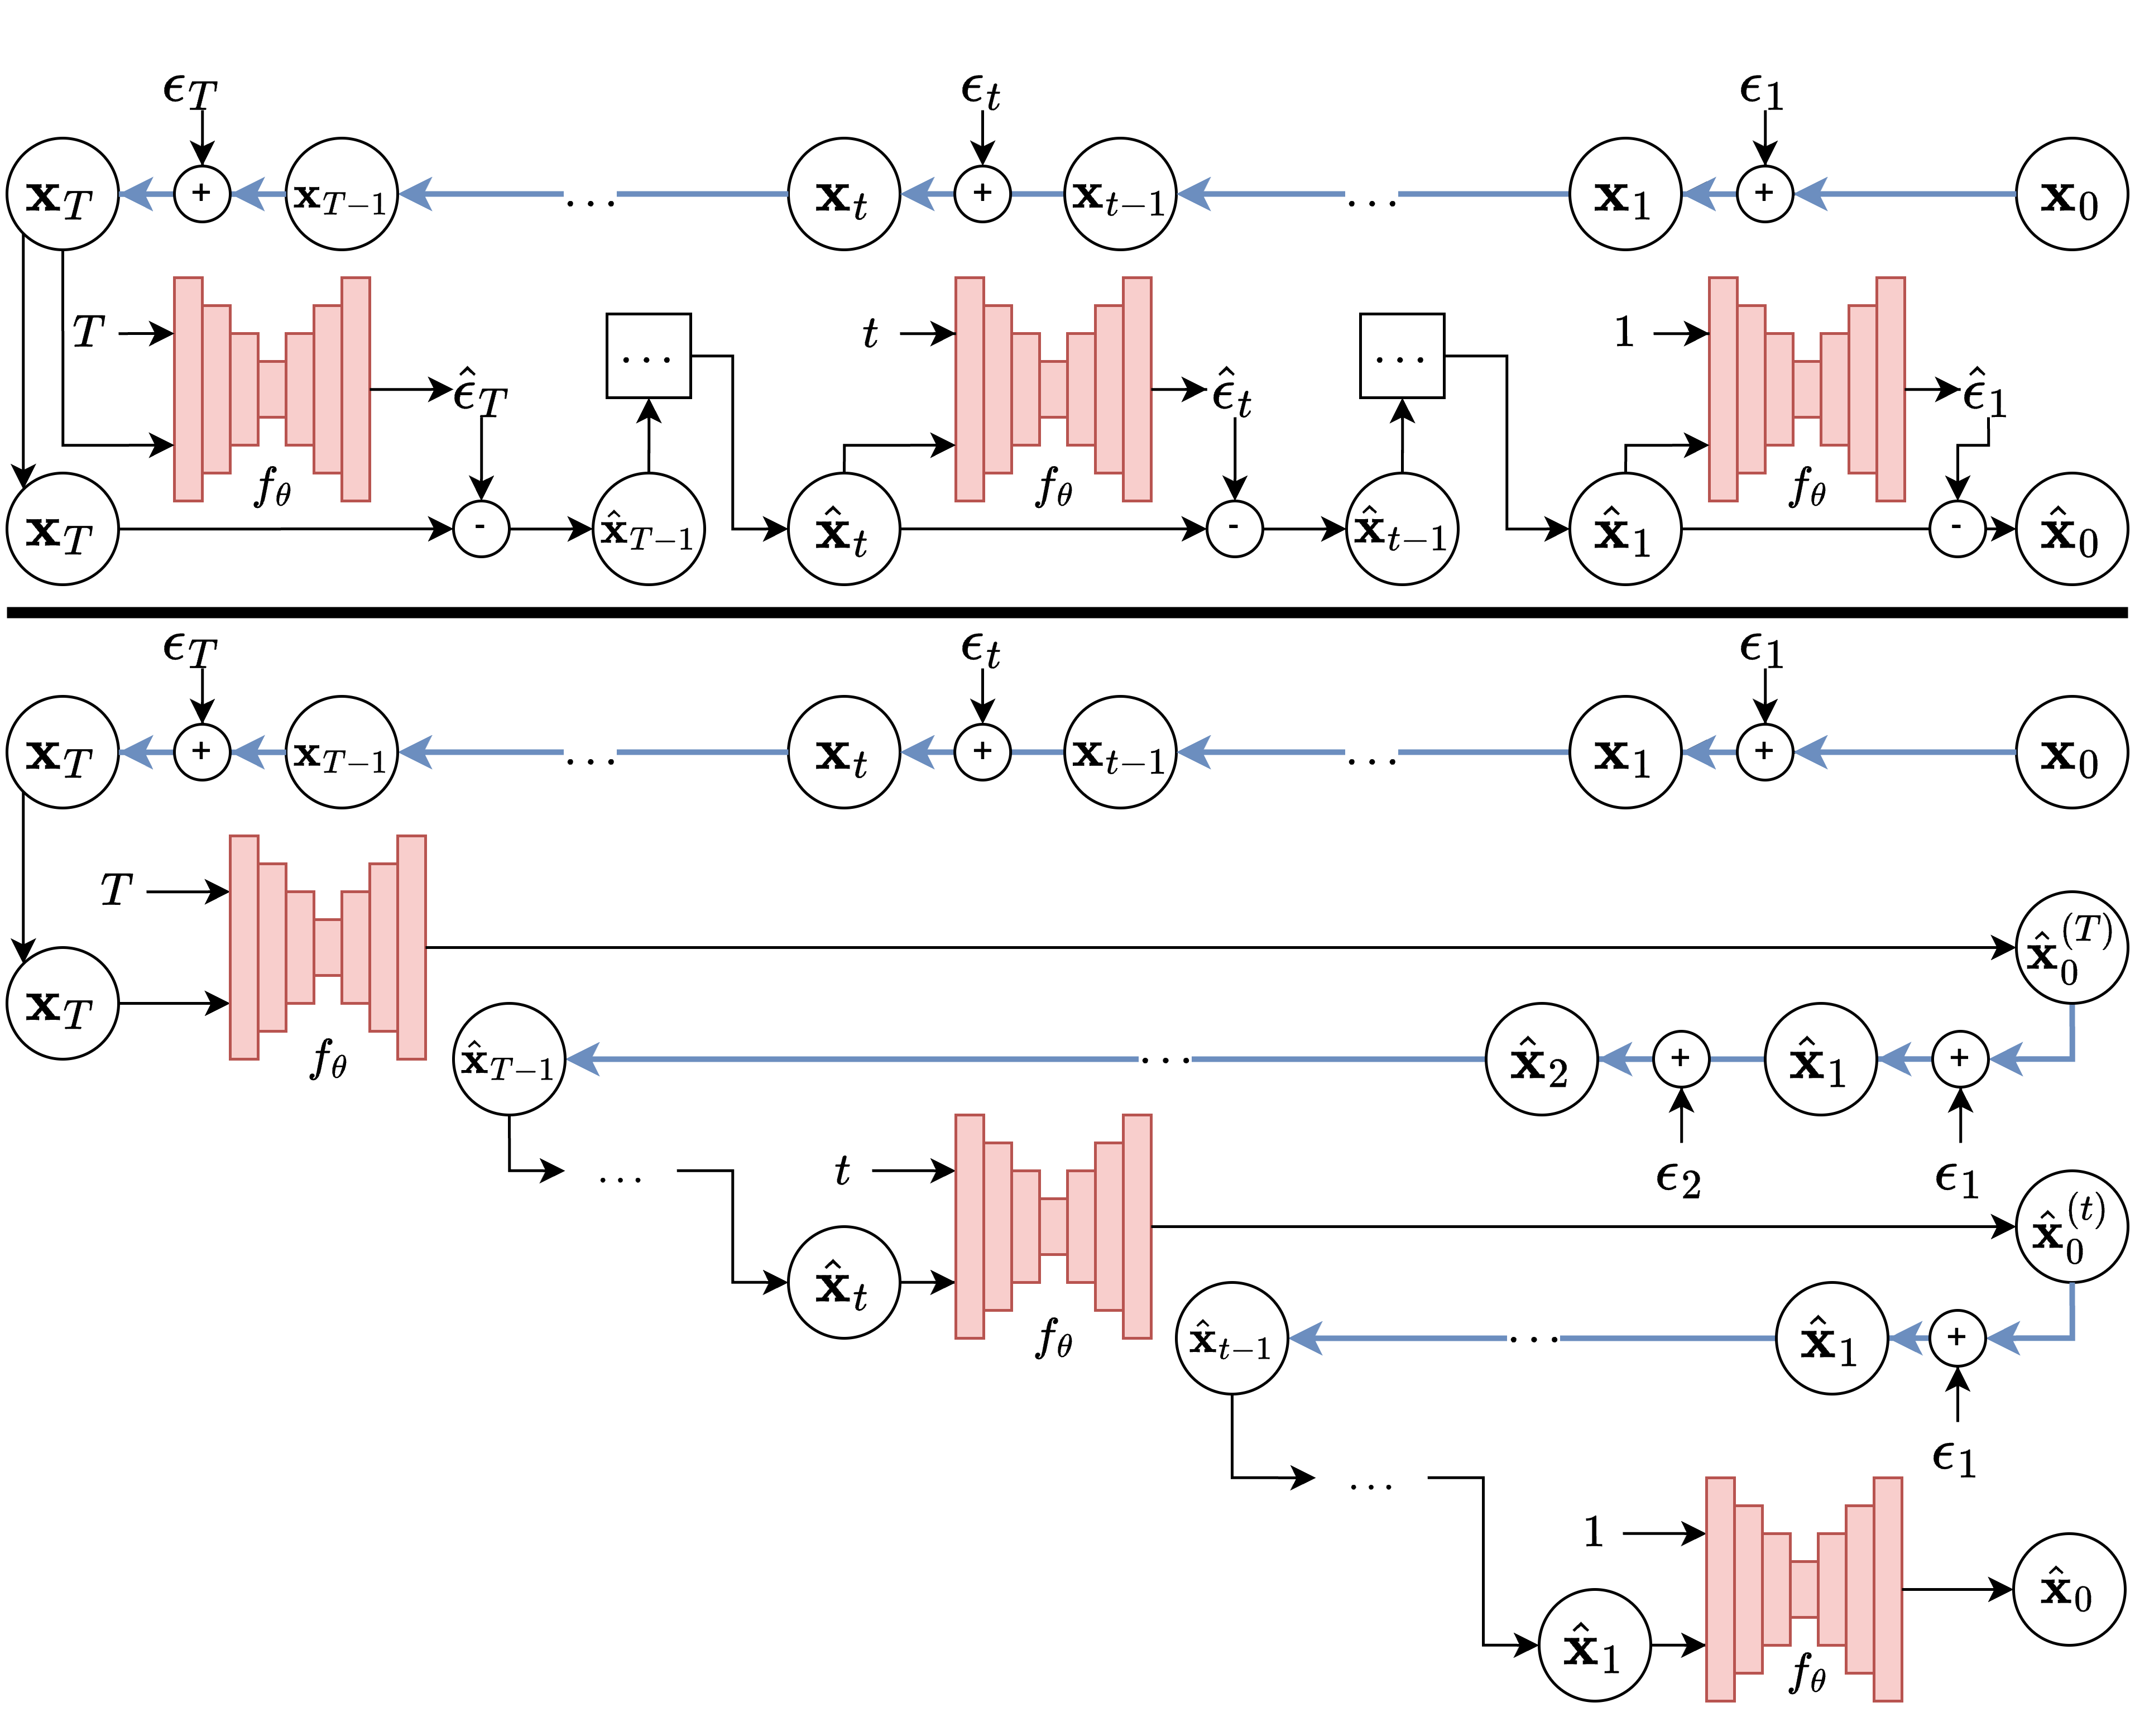
\includegraphics[width=\linewidth]{X0Objective}
	\caption{Comparison between $\epsilon$ objective (top) and $\bx_0$ objective (bottom)}
	\label{fig:X0Objective}
\end{figure}

As shown in \autoref{fig:X0Objective}, we start with forward diffusion from $t: 1 \rightarrow T$ to obtain $\bx_T \sim \mathcal{N} (0, \mathbf{I})$. After acquiring $\bx_T$, we feed it into $f_{\theta}$ to predict $\hat{\bx}_0$, and from $\hat{\bx}_0$ we add noise to obtain $\hat{\bx}_{t-1}$. This continues until $t = 1$, when $\hat{\bx}_0$ is ultimately obtained. We can compare the two methods as follows:

\begin{itemize}
	\item \textbf{$\epsilon$ objective}: the model predicts the noise. Begin with forward noise injection to get $\bx_T$, then use $\bx_T \in \mathcal{N}(0, \mathbf{I})$ as input for denoising. During denoising, the model predicts the noise $\hat{\epsilon}_t$ added in the forward step, i.e., $\epsilon_t$, and minimizes the error between the predicted and actual forward noise.
	\item \textbf{$\bx_0$ objective}: similarly, the model applies forward diffusion to get $\bx_T$, then uses $\bx_T \in \mathcal{N}(0, \mathbf{I})$ for denoising. The model directly predicts $\bx_0$, then reintroduces noise to compute $\bx_{t-1}$, and continues using $\bx_{t-1}$ as input to predict $\bx_0$ again.
\end{itemize}

\subsection{Conditional Diffusion Models}
\label{subsec:DiffusionCondition}

To control the generation process under different conditions, generation must be conditioned on $c$—that is, we aim to model $p(\bx | c)$ given condition $c$. The authors in \cite{dhariwal2021diffusion} proposed using a separate function $f_{\phi}$ to train the conditional component. However, this approach presents difficulties when the conditions change, and combining or updating weights in a separate model is challenging for scalability.

\begin{figure}[h]
	\captionsetup{skip=20pt}
	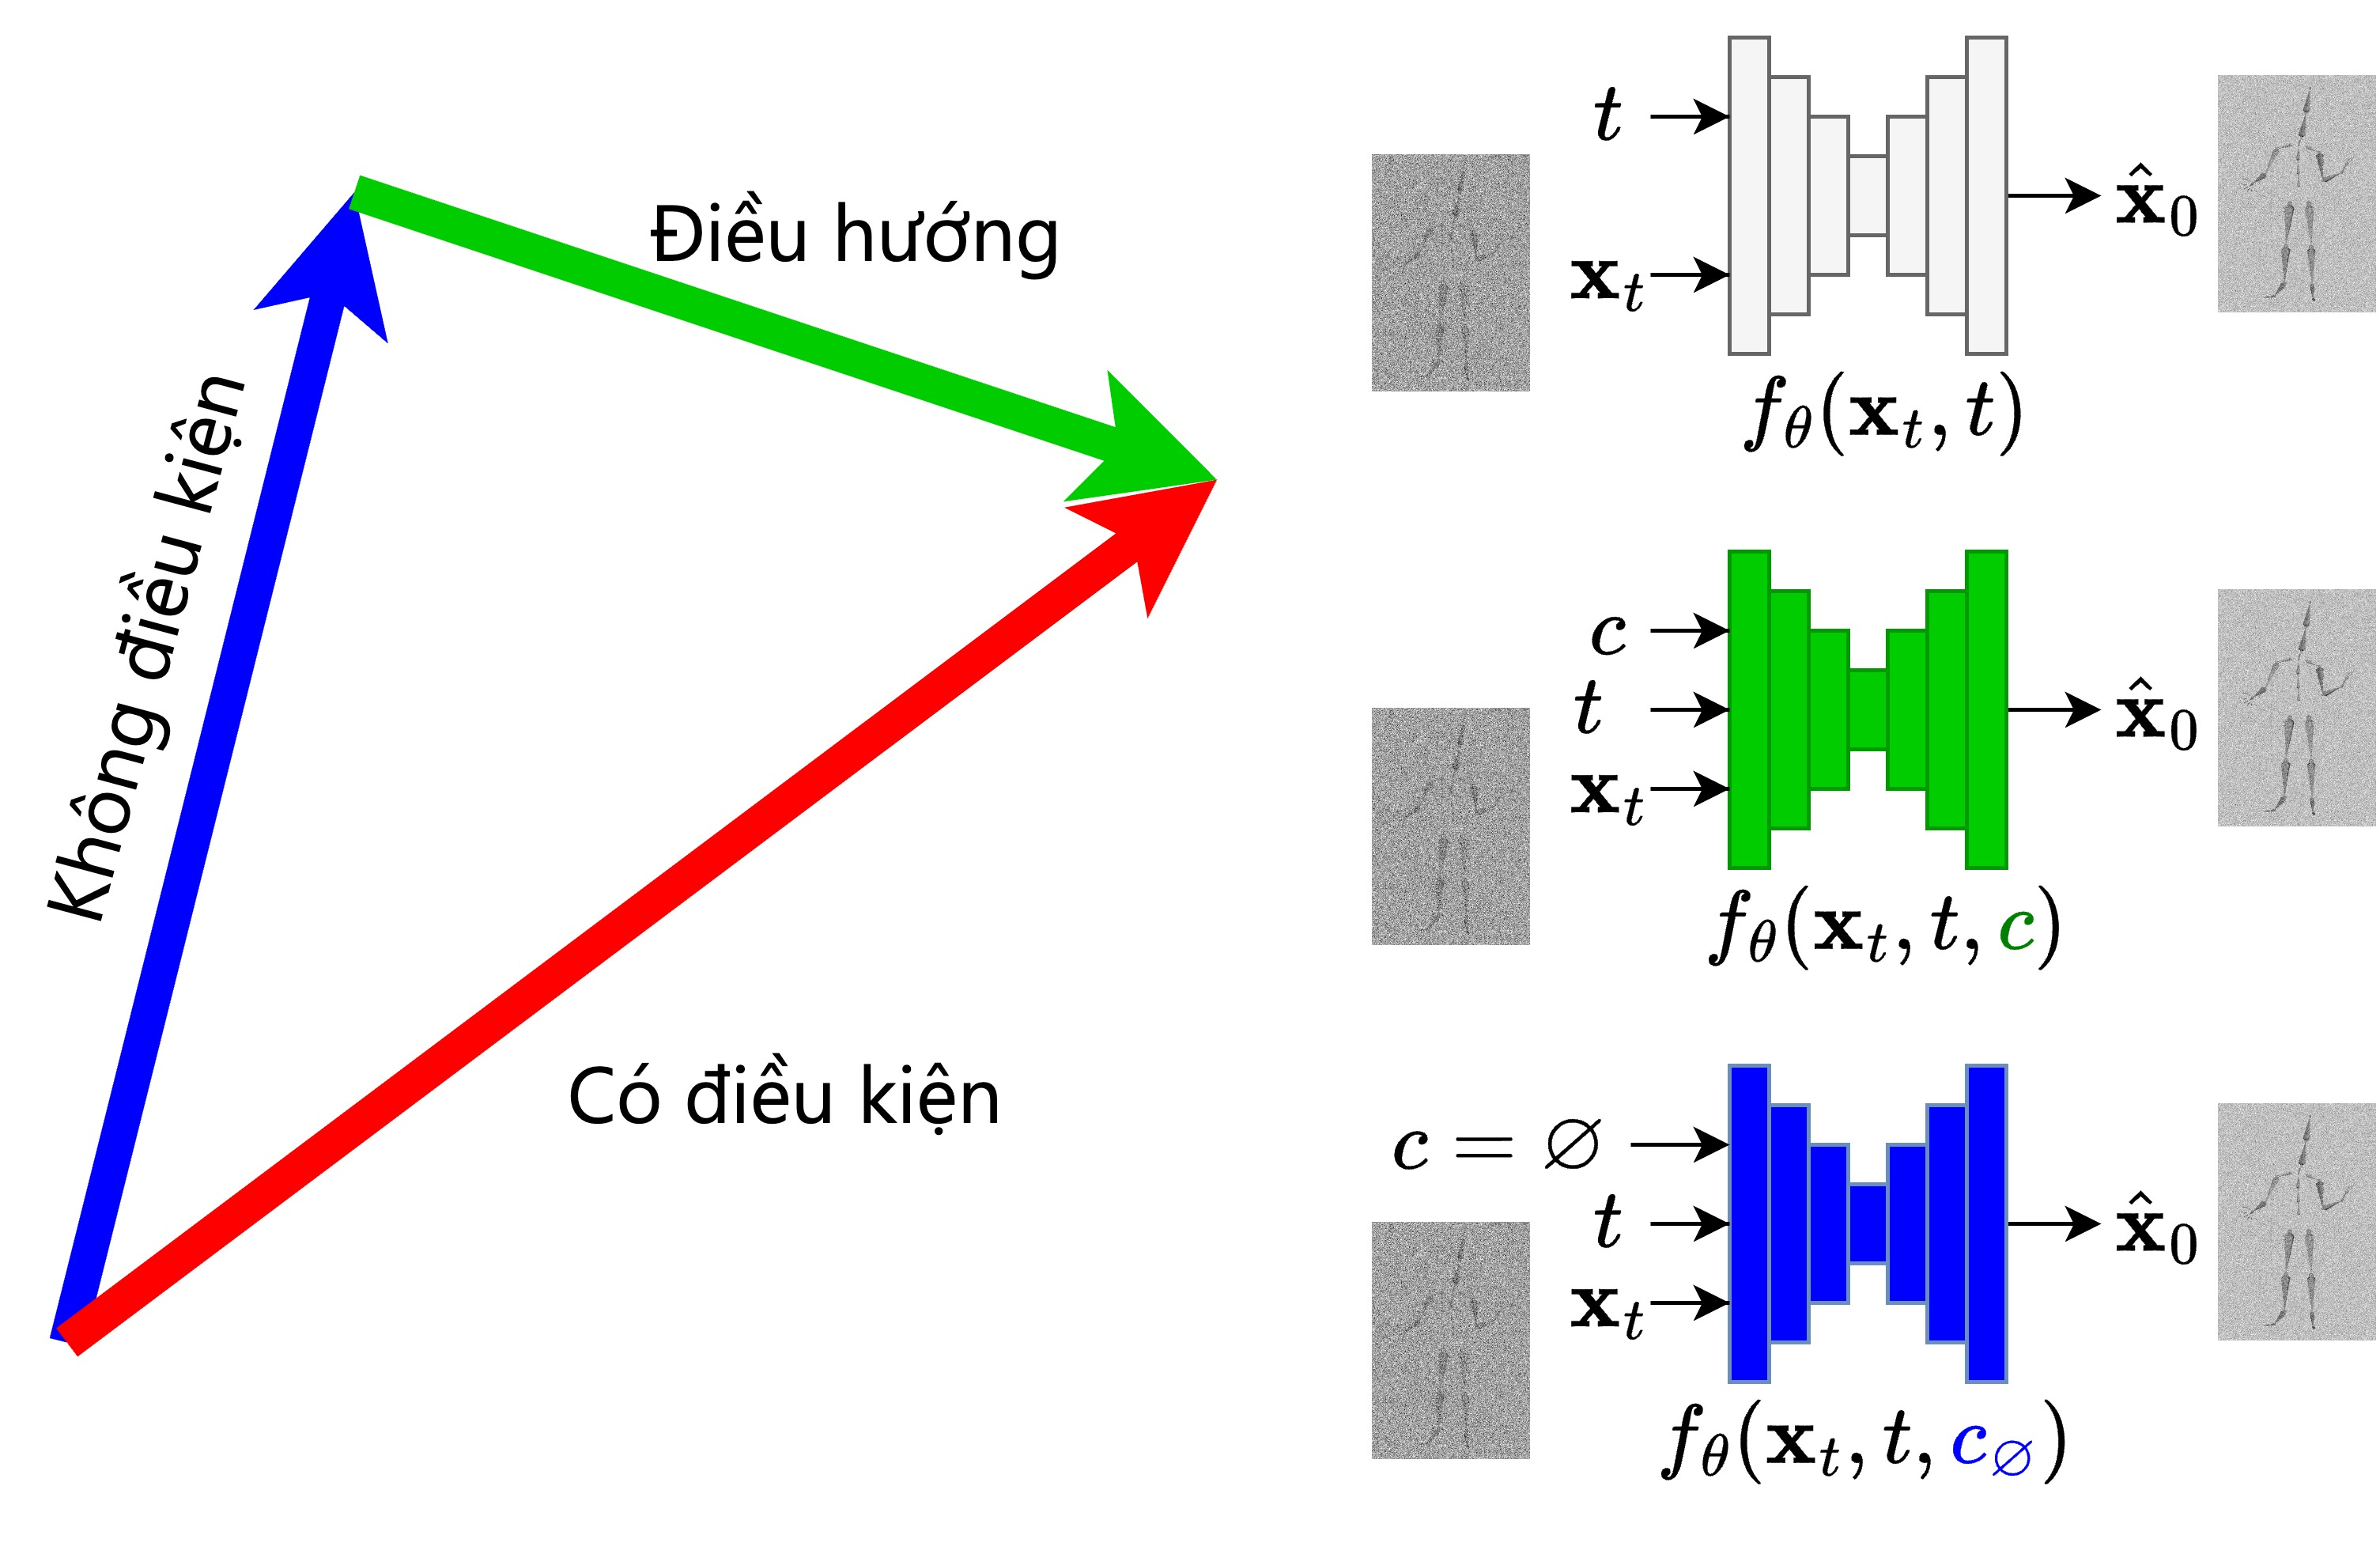
\includegraphics[width=0.9\linewidth]{AdversarialGradient}
	\caption{Conditional Diffusion via Guidance Vector}
	\label{fig:AdversarialGradient}
\end{figure}

As shown in \autoref{fig:GaussianDrift}, to allow inference to generate different $\bx_0$ samples controllably based on condition $c$, a guidance term must be added at each step $t$. The authors proposed Classifier-Free Diffusion Guidance \cite{ho2022classifier}, in which the result $\bx_0$ is updated by combining the conditional and unconditional outputs:

\begin{equation}
{\color{red}{\hat{\mathbf{x}}}}_{0 \gamma, \color{green}{c}, \color{blue}{c_{\varnothing}}}=\gamma \cdot f_{\theta} \left(\mathbf{x}_{t}, t, {\color{green}{c}} \right)+(1-\gamma) \cdot f_{\theta} \left(\mathbf{x}_{t}, t, {\color{blue}{c_{\varnothing}}} \right)
\end{equation}

Here, $c$ is the condition, $c_{\varnothing}$ is the null (empty) condition, and the conditional generation is controlled by the parameter $\gamma$: the larger $\gamma$ is, the closer the result aligns with condition $c$; conversely, a smaller $\gamma$ leads to a result closer to the unconditional output.

As illustrated in \autoref{fig:AdversarialGradient}, the top function $f_{\theta}$ is unconditional, the middle one is conditional diffusion, and the bottom one is diffusion under an empty condition.

%\pagebreak

\section{Proposed OHGesture Model}
\label{sec:ohgesture}

\begin{figure}[h]
	\centering
		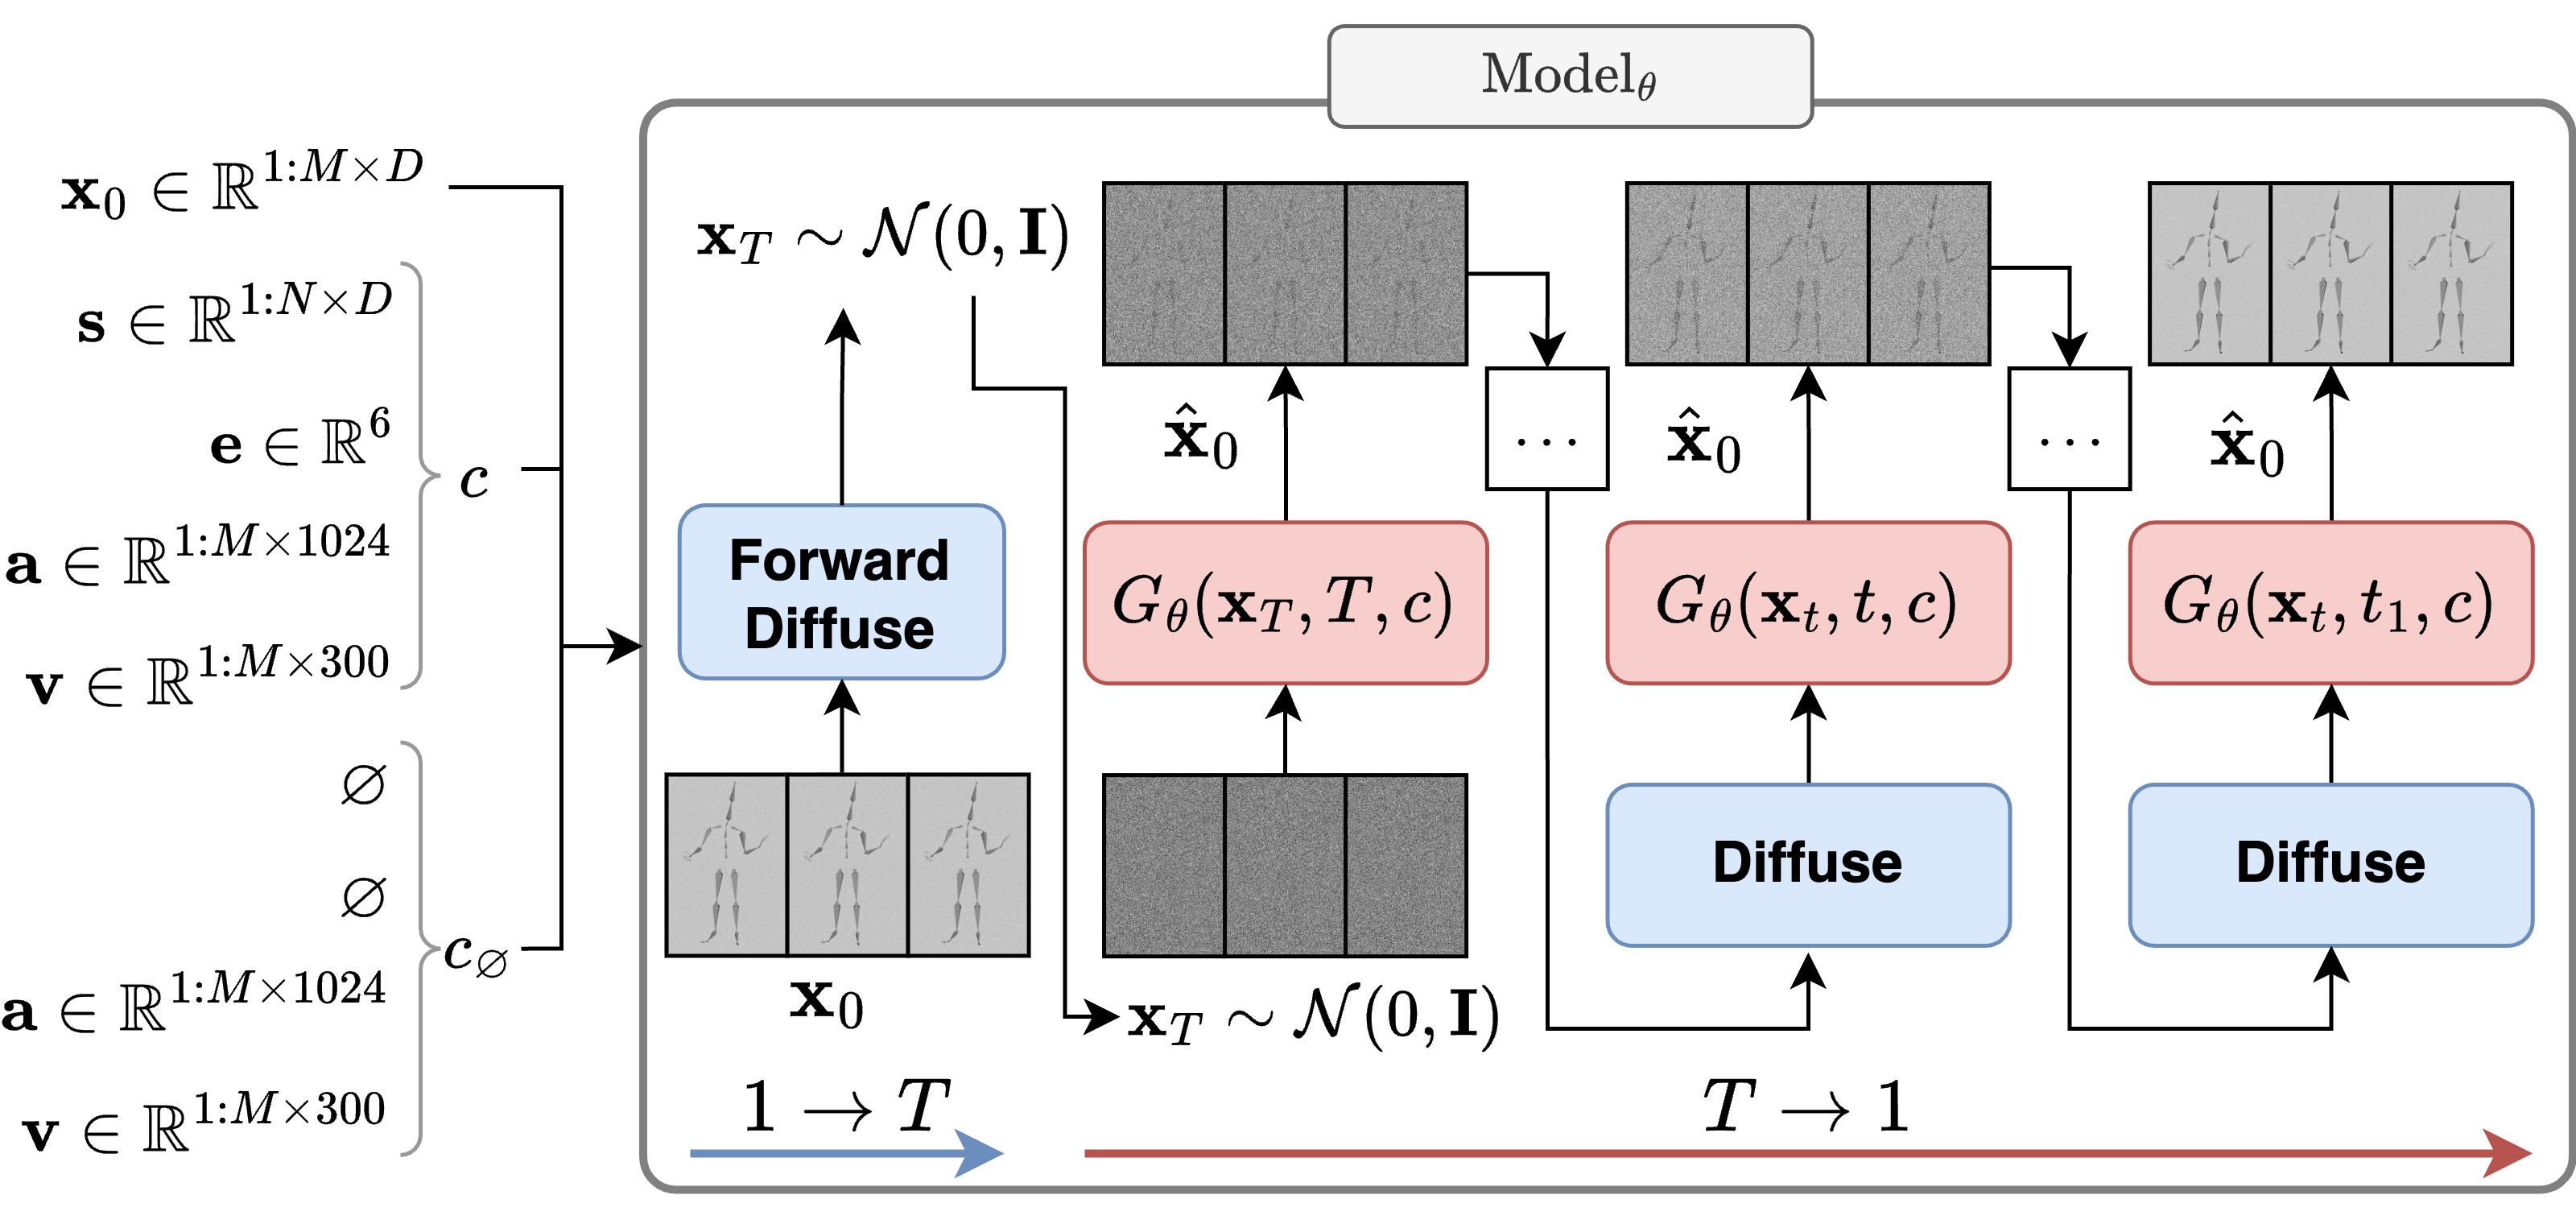
\includegraphics[width=\linewidth]{AllStage}
	\caption{Overview of the OHGesture model}
	\label{fig:TrainingAndSampling}
\end{figure}

The proposed model \textbf{OHGesture} (\textbf{O}pen \textbf{H}uman \textbf{Gesture} Generation) in this thesis is based on the \textbf{DiffuseStyleGesture} model \cite{yang2023diffusestylegesture}, which applies the Diffusion model \cite{ho2020denoising} with conditional guidance \cite{ho2022classifier} (Classifier-Free Diffusion Guidance) to control features during the denoising process.

The similarities and differences of applying the diffusion model to the gesture generation task compared to image generation are as follows:

\vspace{10pt}

\textbf{Similarities}
\begin{itemize}
	\item Uses the Diffusion model (\autoref{sec:summary_diffusion}) on gesture data $\bx^{1:M \times D}$, with $M$ temporal frames and $D=1141$ representing motion coordinates per frame (analogous to image width and height).
	\item Uses conditional Diffusion (\autoref{subsec:DiffusionCondition}) with $\bx_0$ objective (\autoref{subsec:X0Objective}).
	\item In stages \textit{4. Feature Encoding} and \textit{6. Feature Decoding} in \autoref{fig:CommonStage}, the model uses a latent vector of dimension $256$.
\end{itemize}

\textbf{Differences}
\begin{itemize}
	\item Conditional gesture generation:
	\begin{itemize}
		\item Emotional condition: $c = \big[ \mathbf{s}, \mathbf{e}, \mathbf{a}, \mathbf{v} \big]$ and $c_{\varnothing} = \big[ \varnothing, \varnothing, \mathbf{a}, \mathbf{v}\big]$.
		\item Emotion state interpolation between $\mathbf{e}_1, \mathbf{e}_2$ using: $c = \big[ \mathbf{s}, \mathbf{e}_1, \mathbf{a}, \mathbf{v} \big]$ and $c_{\varnothing} = \big[ \mathbf{s}, \mathbf{e}_2, \mathbf{a}, \mathbf{v} \big]$.
	\end{itemize}
	\item In stage \textit{5. Feature Fusion} \autoref{fig:CommonStage}, the model uses Self-Attention: learning the relationship between emotions, seed gestures, and each frame (similar to DALL-E 2's text-image alignment).
	\item In stage \textit{5. Feature Fusion} \autoref{fig:CommonStage}, the model concatenates speech and text (analogous to ControlNet's pixel-wise condition).
\end{itemize}

Here, $\bx_0$ is a sequence of $M$ gesture frames $\mathbf{x} \in \mathbb{R}^{1:M \times D}$ ($D = 1141$), with condition $c = [\mathbf{s}, \mathbf{e}, \mathbf{a}, \mathbf{v}]$ including seed gesture $\mathbf{s}$, emotion $\mathbf{e}$, speech $\mathbf{a}$ corresponding to the gesture, and text $\mathbf{v}$.

The model's objective is to learn parameters $\theta$ of the generative function $G_{\theta}$ with inputs being the noisy gesture matrix $\bx_t \in \mathbb{R}^{1:M \times D}$, timestep $t$, and condition $c$. An overview of the proposed \textbf{OHGesture} model is illustrated in \autoref{fig:TrainingAndSampling}. As with standard diffusion models, it includes two processes: the diffusion process $q$ and the denoising process $p_{\theta}$ with weights $\theta$. The \textit{1. Preprocessing} stage will be presented in \autoref{sec:Preprocessing}.


\subsection{Feature Processing Stage}

In the \textit{Stage 2: Feature Processing} step (\autoref{fig:CommonStage}), the goal is to convert raw input data into matrices or vectors suitable for input into the model.

\begin{itemize}
    \item \textbf{Text} $\mathbf{v} \in \mathbb{R}^{1:M \times 300}$:  
    As discussed in \autoref{subsec:TypicalMethod}, methods such as \textit{MDM} \cite{tevet2022human} and \textit{DiffuseStyleGesture+} \cite{yang2022DiffuseStyleGestureplus} use gesture-descriptive prompts, similar to those used in Midjourney, as input for the model. However, such prompts are mainly used to cluster gestures rather than align them semantically. 

    In contrast, this thesis treats text as a semantic feature that aligns specific segments of text with corresponding gesture segments for digital human generation. Therefore, the contribution in this stage is to use speech data that has already been preprocessed (see \autoref{sec:Preprocessing}) to obtain transcribed text. The FastText model \cite{bojanowski2017enriching} is used to embed this text into vectors, which are then temporally aligned with the number of gesture frames, resulting in a text matrix $\mathbf{v} \in \mathbb{R}^{1:M \times 300}$. For segments without text, zero vectors are used; for segments with vocabulary, the corresponding embedding is assigned for each gesture frame.

    \item \textbf{Speech} $\mathbf{a} \in \mathbb{R}^{1:M \times 1024}$:  
    All speech data in `.wav` format is downsampled to $16~\mathrm{kHz}$. The speech corresponding to the gesture segment (4 seconds) is extracted as a waveform vector $\mathbf{a} \in \mathbb{R}^{64000}$. Following DiffuseStyleGesture, this thesis uses the pre-trained WavLM Large model \cite{Chen_2022} to embed the raw waveform into a high-dimensional vector representing acoustic features. Linear interpolation is then applied to temporally align the latent features from WavLM at $20~\text{fps}$, resulting in the speech matrix $\mathbf{a} \in \mathbb{R}^{1:M \times 1024}$.

    \item \textbf{Emotion} $\mathbf{e} \in \mathbb{R}^{6}$:  
    Emotion is represented by one of six classes: $\texttt{Happy}$, $\texttt{Sad}$, $\texttt{Neutral}$, $\texttt{Old}$, $\texttt{Relaxed}$, and $\texttt{Angry}$.  
    Each label is encoded using one-hot encoding to form the vector $\mathbf{e} \in \mathbb{R}^{6}$.

    \item \textbf{Seed Gesture} $\mathbf{s} \in \mathbb{R}^{1:N \times D}$:  
    This is the initial gesture sequence composed of $N=8$ frames, with each frame containing joint data for 75 joints. These are processed according to the formula in \autoref{eq:gesturevector} to yield a $D=1141$-dimensional vector.

    \item \textbf{Ground Truth Gesture} $\mathbf{x}_{0} \in \mathbb{R}^{1:M \times D}$:  
    This is the ground-truth gesture sequence of $M = 80$ frames (corresponding to 4 seconds at $20~\text{fps}$), which is preprocessed to form the matrix $\mathbf{x}_{0} \in \mathbb{R}^{1:M \times D}$.
\end{itemize}

\subsection{Feature Extraction Stage}
\label{subsec:feature_extraction}

In the \textit{Stage 3: Feature Extraction} step (\autoref{fig:CommonStage}), the goal is to convert the input matrices into latent vectors that capture the semantic content of each modality. This is done by passing the feature data through linear transformation layers or Multilayer Perceptrons (MLPs).


\begin{figure}[H]
	\centering
	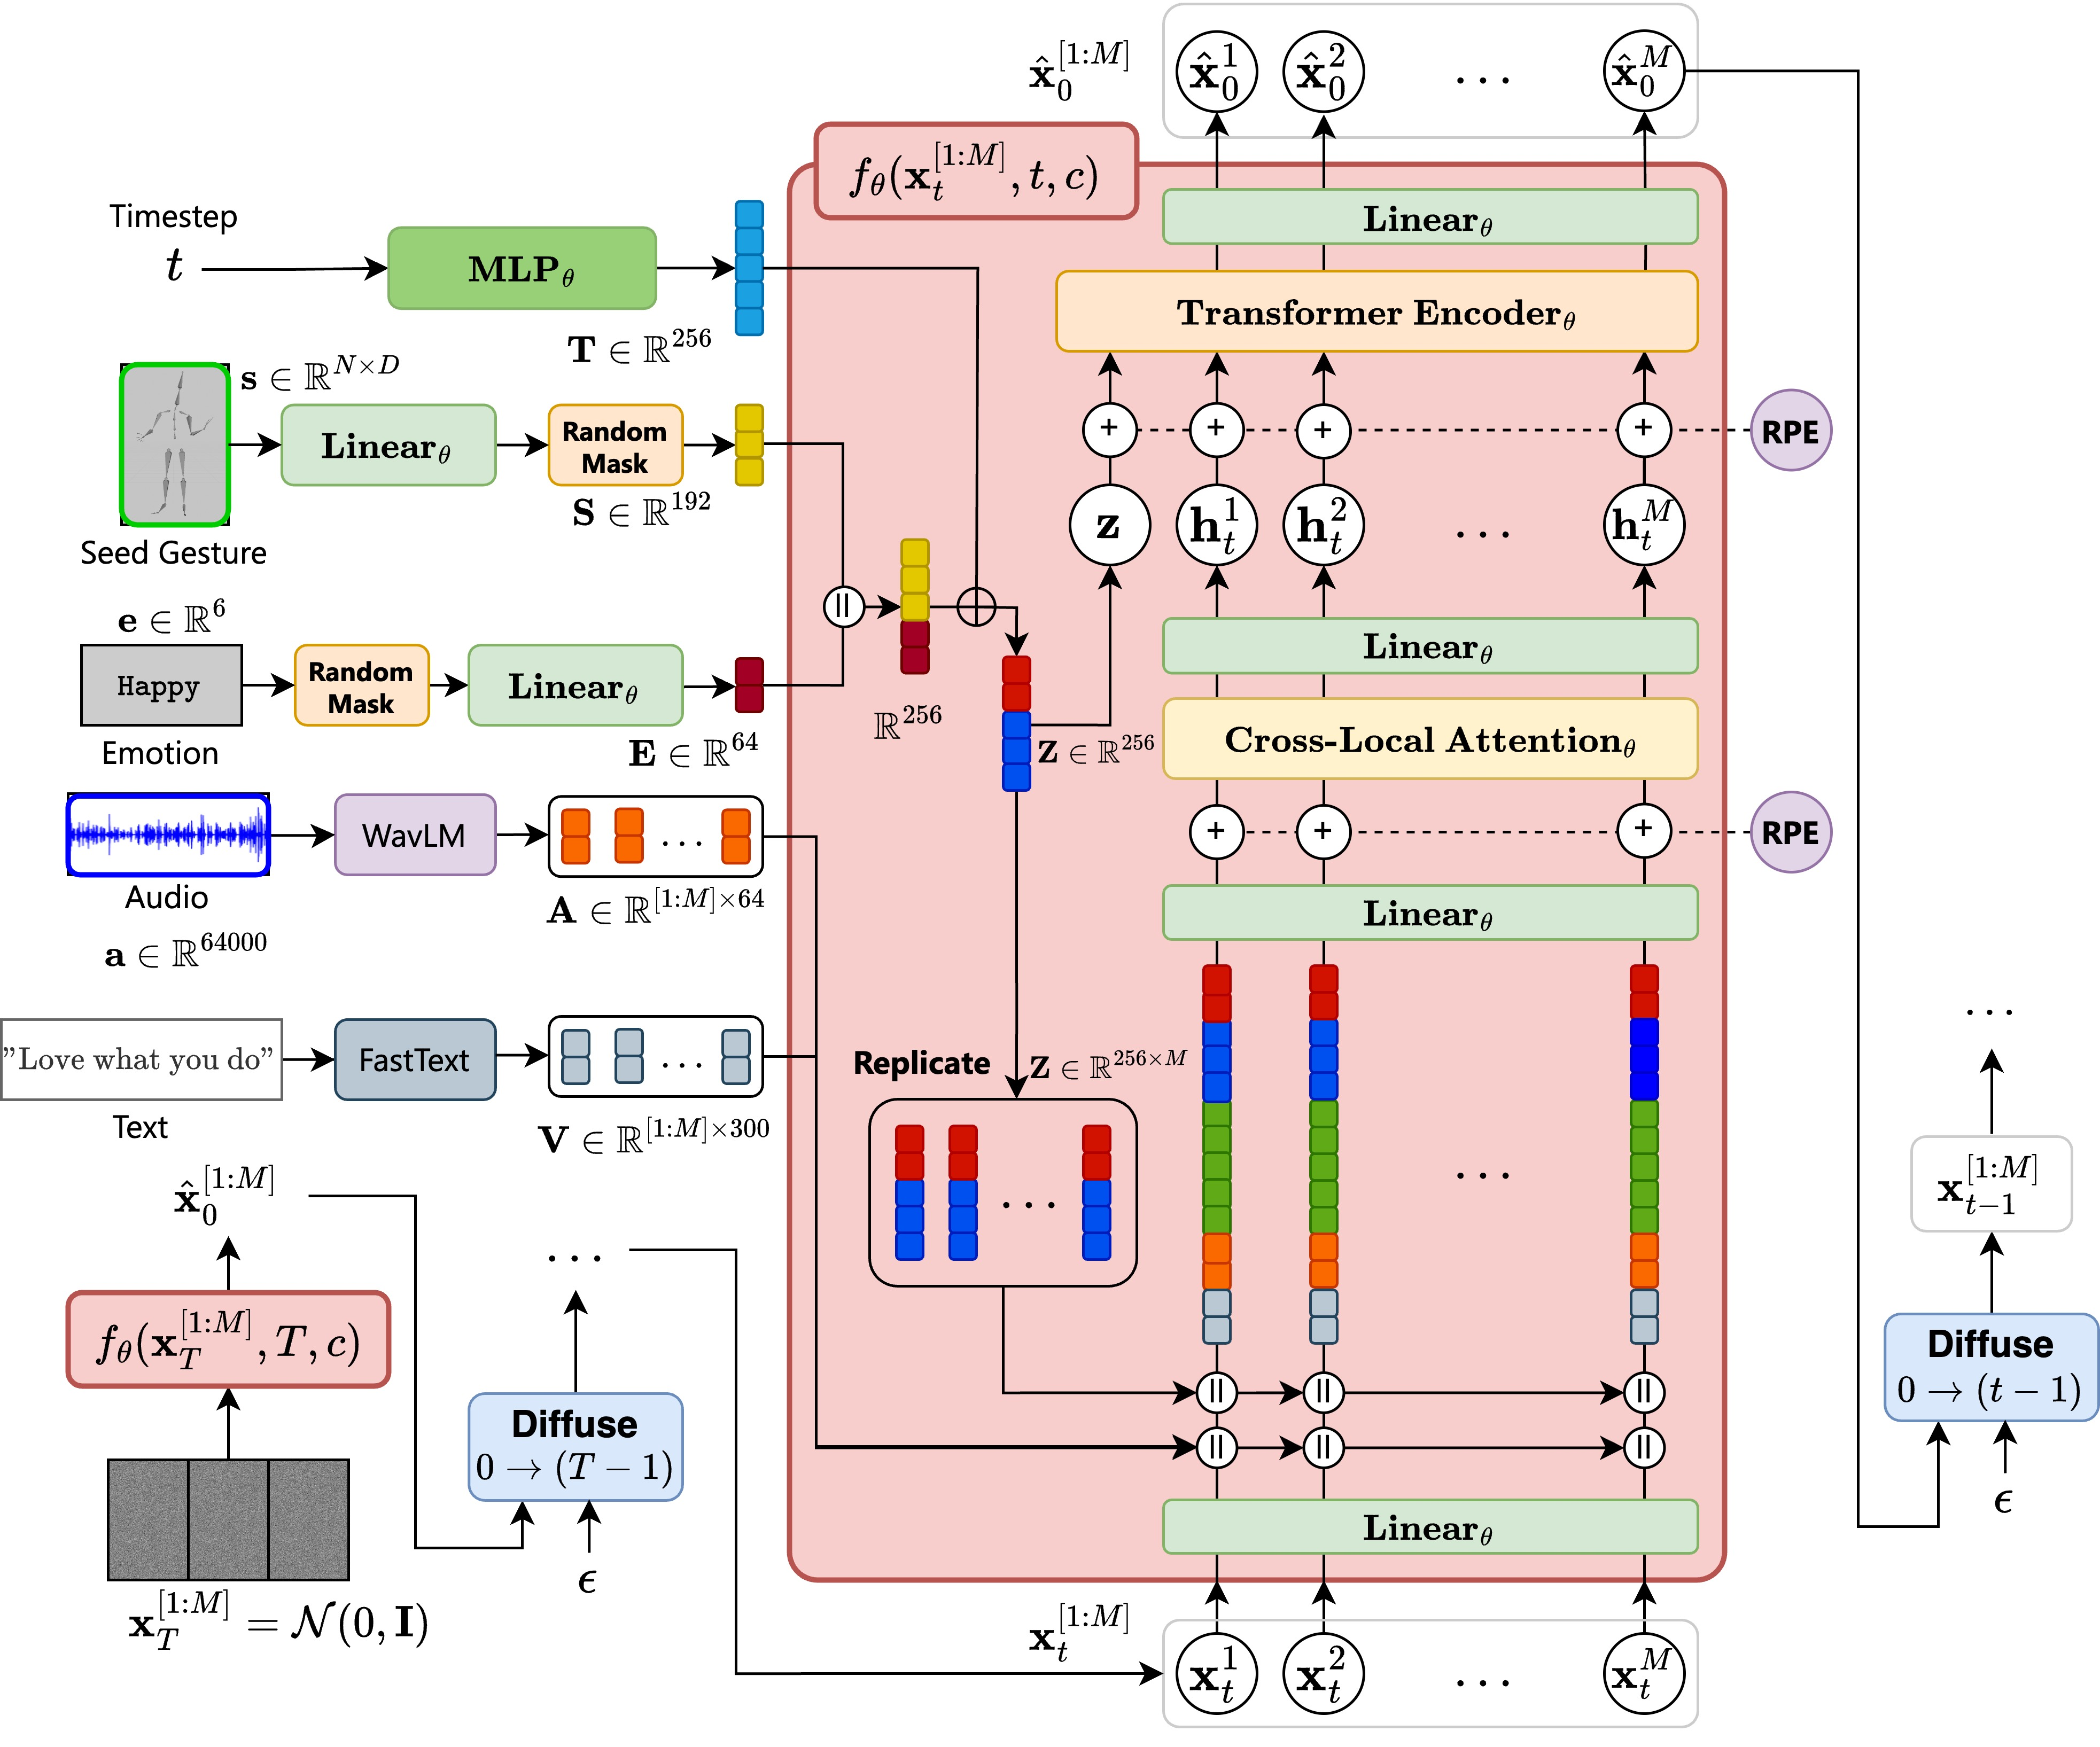
\includegraphics[width=\textwidth]{OHGesture}
	\caption{The Model Architecture in OHGesture}
	\label{fig:OHGesture}
\end{figure}
\vspace{-10pt}

\begin{itemize}
    \item \textbf{Timestep $\mathbf{T} \in \mathbb{R}^{256}$}: The timestep at each process step $t \in [0, T]$ enables the model to generalize the denoising process across different time steps. The objective is for the model to learn how the values should change with respect to $t$ in order to accurately predict $\bx_0$. The timestep $t$ is initialized using sinusoidal positional encoding: $\text{PE}(t) = \left[ \sin{\left(\frac{t}{10000^{2i / d}}\right)}, \cos{\left(\frac{t}{10000^{2i / d}}\right)} \right]$, and then passed through a Multilayer Perceptron (MLP) to obtain the vector $\mathbf{T} \in \mathbb{R}^{256}$.

    \item \textbf{Speech $\mathbf{A} \in \mathbb{R}^{1:M \times 64}$}: The speech feature matrix $\mathbf{a} \in \mathbb{R}^{1:M \times 1024}$ is passed through a linear layer to reduce its dimensionality to a 64-dimensional feature vector, resulting in the matrix $\mathbf{A} \in \mathbb{R}^{1:M \times 64}$.

    \item \textbf{Text $\mathbf{V} \in \mathbb{R}^{1:M \times 64}$}: After preprocessing described in \autoref{sec:Preprocessing}, the text is aligned to match the number of frames $M$, resulting in matrix $\mathbf{v} \in \mathbb{R}^{1:M \times 300}$. It is then passed through a linear transformation to reduce feature dimensionality, yielding the final matrix $\mathbf{V} \in \mathbb{R}^{1:M \times 64}$, aligned with the speech matrix.

    \item \textbf{Seed Gesture $\mathbf{S} \in \mathbb{R}^{192}$}: The seed gesture $\mathbf{s} \in \mathbb{R}^{1:N \times D}$ is processed through a linear transformation layer to obtain the vector $\mathbf{S} \in \mathbb{R}^{192}$. During training, $\mathbf{S}$ is also passed through a random masking layer to randomly mask segments of gesture frames in $N$ frames. This allows the model to learn how missing frames impact the final predicted gestures.

    \item \textbf{Emotion $\mathbf{E} \in \mathbb{R}^{64}$}: The emotion vector $\mathbf{e} \in \mathbb{R}^{6}$ is passed through a linear transformation layer to produce the feature vector $\mathbf{E} \in \mathbb{R}^{64}$. This is designed to be concatenated with the seed gesture vector $\mathbf{S} \in \mathbb{R}^{192}$ to form a 256-dimensional latent vector.

    \item \textbf{Noisy Gesture $\mathbf{x}_{T} \in \mathbb{R}^{1:M \times D}$}: During training, $\mathbf{x}_t$ is the noisy gesture that shares the same dimensionality as the original gesture $\mathbf{x}_0$ and is sampled from a standard normal distribution $\mathcal{N}(0, \mathbf{I})$. The initial noisy gesture $\mathbf{x}_T$ is drawn from a Gaussian distribution, and the subsequent $\mathbf{x}_t, \, t < T$ are produced through iterative noising steps, as illustrated in \autoref{fig:TrainingAndSampling}.
%   Afterward, the dimensionality is adjusted to 256 using a linear transformation layer.
\end{itemize}


\subsection{Feature Encoding Stage}

In the \textit{Stage 4: Feature Encoding} step (\autoref{fig:CommonStage}), the objective is to reduce the dimensionality of the input data to a lower latent space, in order to alleviate computational overhead and avoid the explosion of processing complexity.

The primary data used in the diffusion process is the gesture sequence $\bx_t \in \mathbb{R}^{1:M \times D}$. As illustrated in \autoref{fig:OHGesture}, the gesture sequence with size $M \times D$ is passed through a linear transformation layer $\operatorname{Linear}_{\theta}$ to produce the matrix $\mathbf{X} \in \mathbb{R}^{1:M \times 256}$. This dimensionality reduction of $\bx$ is performed prior to passing the gesture sequence through the Cross-Local Attention and Transformer Encoder layers, in order to compute correlations across multiple modalities.

\subsection{Feature Fusion Stage}

In the \textit{Stage 5: Feature Fusion} step (\autoref{fig:CommonStage}), the goal is to compute inter-feature correlations using concatenation, addition, or attention-based mechanisms.

First, the seed gesture vector $\mathbf{S} \in \mathbb{R}^{192}$ and the emotion vector $\mathbf{E} \in \mathbb{R}^{64}$ are concatenated to form a single vector of size $256$, since $256$ is the chosen hidden dimensionality for computing feature correlations. This vector is then added to the timestep vector $\mathbf{T}$ to form the final vector $\mathbf{z}_{tk} \in \mathbb{R}^{256}$.


\begin{equation}
	\label{eq:ConditionConcat}
	\mathbf{z}_{tk} = \operatorname{concat }(\mathbf{E}\ || \  \mathbf{S}) + \mathbf{T}
\end{equation}

The feature fusion process of $\mathbf{z}_{tk}$ is illustrated in \autoref{fig:FeatureFusion}.

\subsubsection{Frame-wise Feature Integration}

Next, $\mathbf{z}_{tk} \xrightarrow{\operatorname{replicate}} \mathbf{Z}$ is replicated $M$ times to match the dimensionality of $M$ frames, resulting in the matrix $\mathbf{Z} \in \mathbb{R}^{1:M \times 256}$, as shown in \autoref{fig:OHGesture}.

The speech feature matrix $\mathbf{A}$ and the text feature matrix $\mathbf{V}$ are then added together to produce a matrix that combines both modalities. This combined matrix is then concatenated with the gesture feature matrix $\mathbf{X}$. Finally, the result is concatenated with matrix $\mathbf{Z}$ to obtain the full feature matrix $\mathbf{M}$.


\begin{equation}
	\label{eq:FrameConcat}
	\mathbf{M} = \operatorname{concat}( \mathbf{Z}\  || \   \operatorname{concat}(\mathbf{X}\ || \  (\mathbf{V} + \mathbf{A}) ) )
\end{equation}

The matrix $\mathbf{M} \in \mathbb{R}^{1:M \times P}$, as shown in \autoref{eq:FrameConcat}, represents the frame-wise feature matrix from frame $1$ to frame $M$, where each frame has dimensionality $P$, which is the sum of all concatenated feature vectors. Given $\mathbf{X} \in \mathbb{R}^{1:M \times 256}$, $\mathbf{Z} \in \mathbb{R}^{1:M \times 256}$, and $\mathbf{A}, \mathbf{V} \in \mathbb{R}^{1:M \times 64}$, the resulting dimensionality is $P = 256 + 256 + 64$.

Subsequently, the matrix $\mathbf{m}$ is passed through a linear transformation to reduce its dimensionality from $P$ to $256$, resulting in the matrix $\mathbf{m}_{t} \in \mathbb{R}^{1:M \times 256}$.

\begin{equation}
	\label{eq:FeatureDimensionReducion}
	\mathbf{m}_{t} = \operatorname{Linear}_{\theta}( \mathbf{M} )
\end{equation}

\subsubsection{Attention Mechanism in the Feature Integration Process}

In the proposed model, the attention mechanism \cite{vaswani2017attention} is employed to integrate features. The objective of applying attention is to capture the correlation between individual frames in the sequence. The attention mechanism is utilized in both the Cross-Local Attention and the Self-Attention layers within the Transformer Encoder.

The attention mechanism is formulated as follows:

\begin{equation} \label{eq:attention}
	\operatorname{Attention}(\mathbf{Q}, \mathbf{K}, \mathbf{V}, \mathbf{Mask})=\operatorname{softmax}\left(\frac{\mathbf{Q} \mathbf{K}^{T}+\mathbf{Mask}}{\sqrt{C}}\right) \mathbf{V}
\end{equation}

In the Attention formula above, $\mathbf{Q}$ (Query), $\mathbf{K}$ (Key), and $\mathbf{V}$ (Value) are matrices obtained by passing the input through linear transformation matrices: $\mathbf{Q} = {X} \mathbf{W}_Q$, $\mathbf{K} = {X} \mathbf{W}_K$, $\mathbf{V} = {X} \mathbf{W}_V$. The input $X$ is a matrix representing a sequence of $M$ frames, where each frame is a concatenated vector composed of various feature vectors, including seed gestures, text, speech, emotion, and the gesture $\bx_t$ that the thesis aims to denoise. The term $\sqrt{C}$ is a normalization \textbf{c}onstant that accounts for the dimensionality of the matrices. 

The Local-Cross Attention mechanism is controlled to focus only on local motion features of gestures and features in neighboring frames.

\begin{figure}[H]
	\centering
	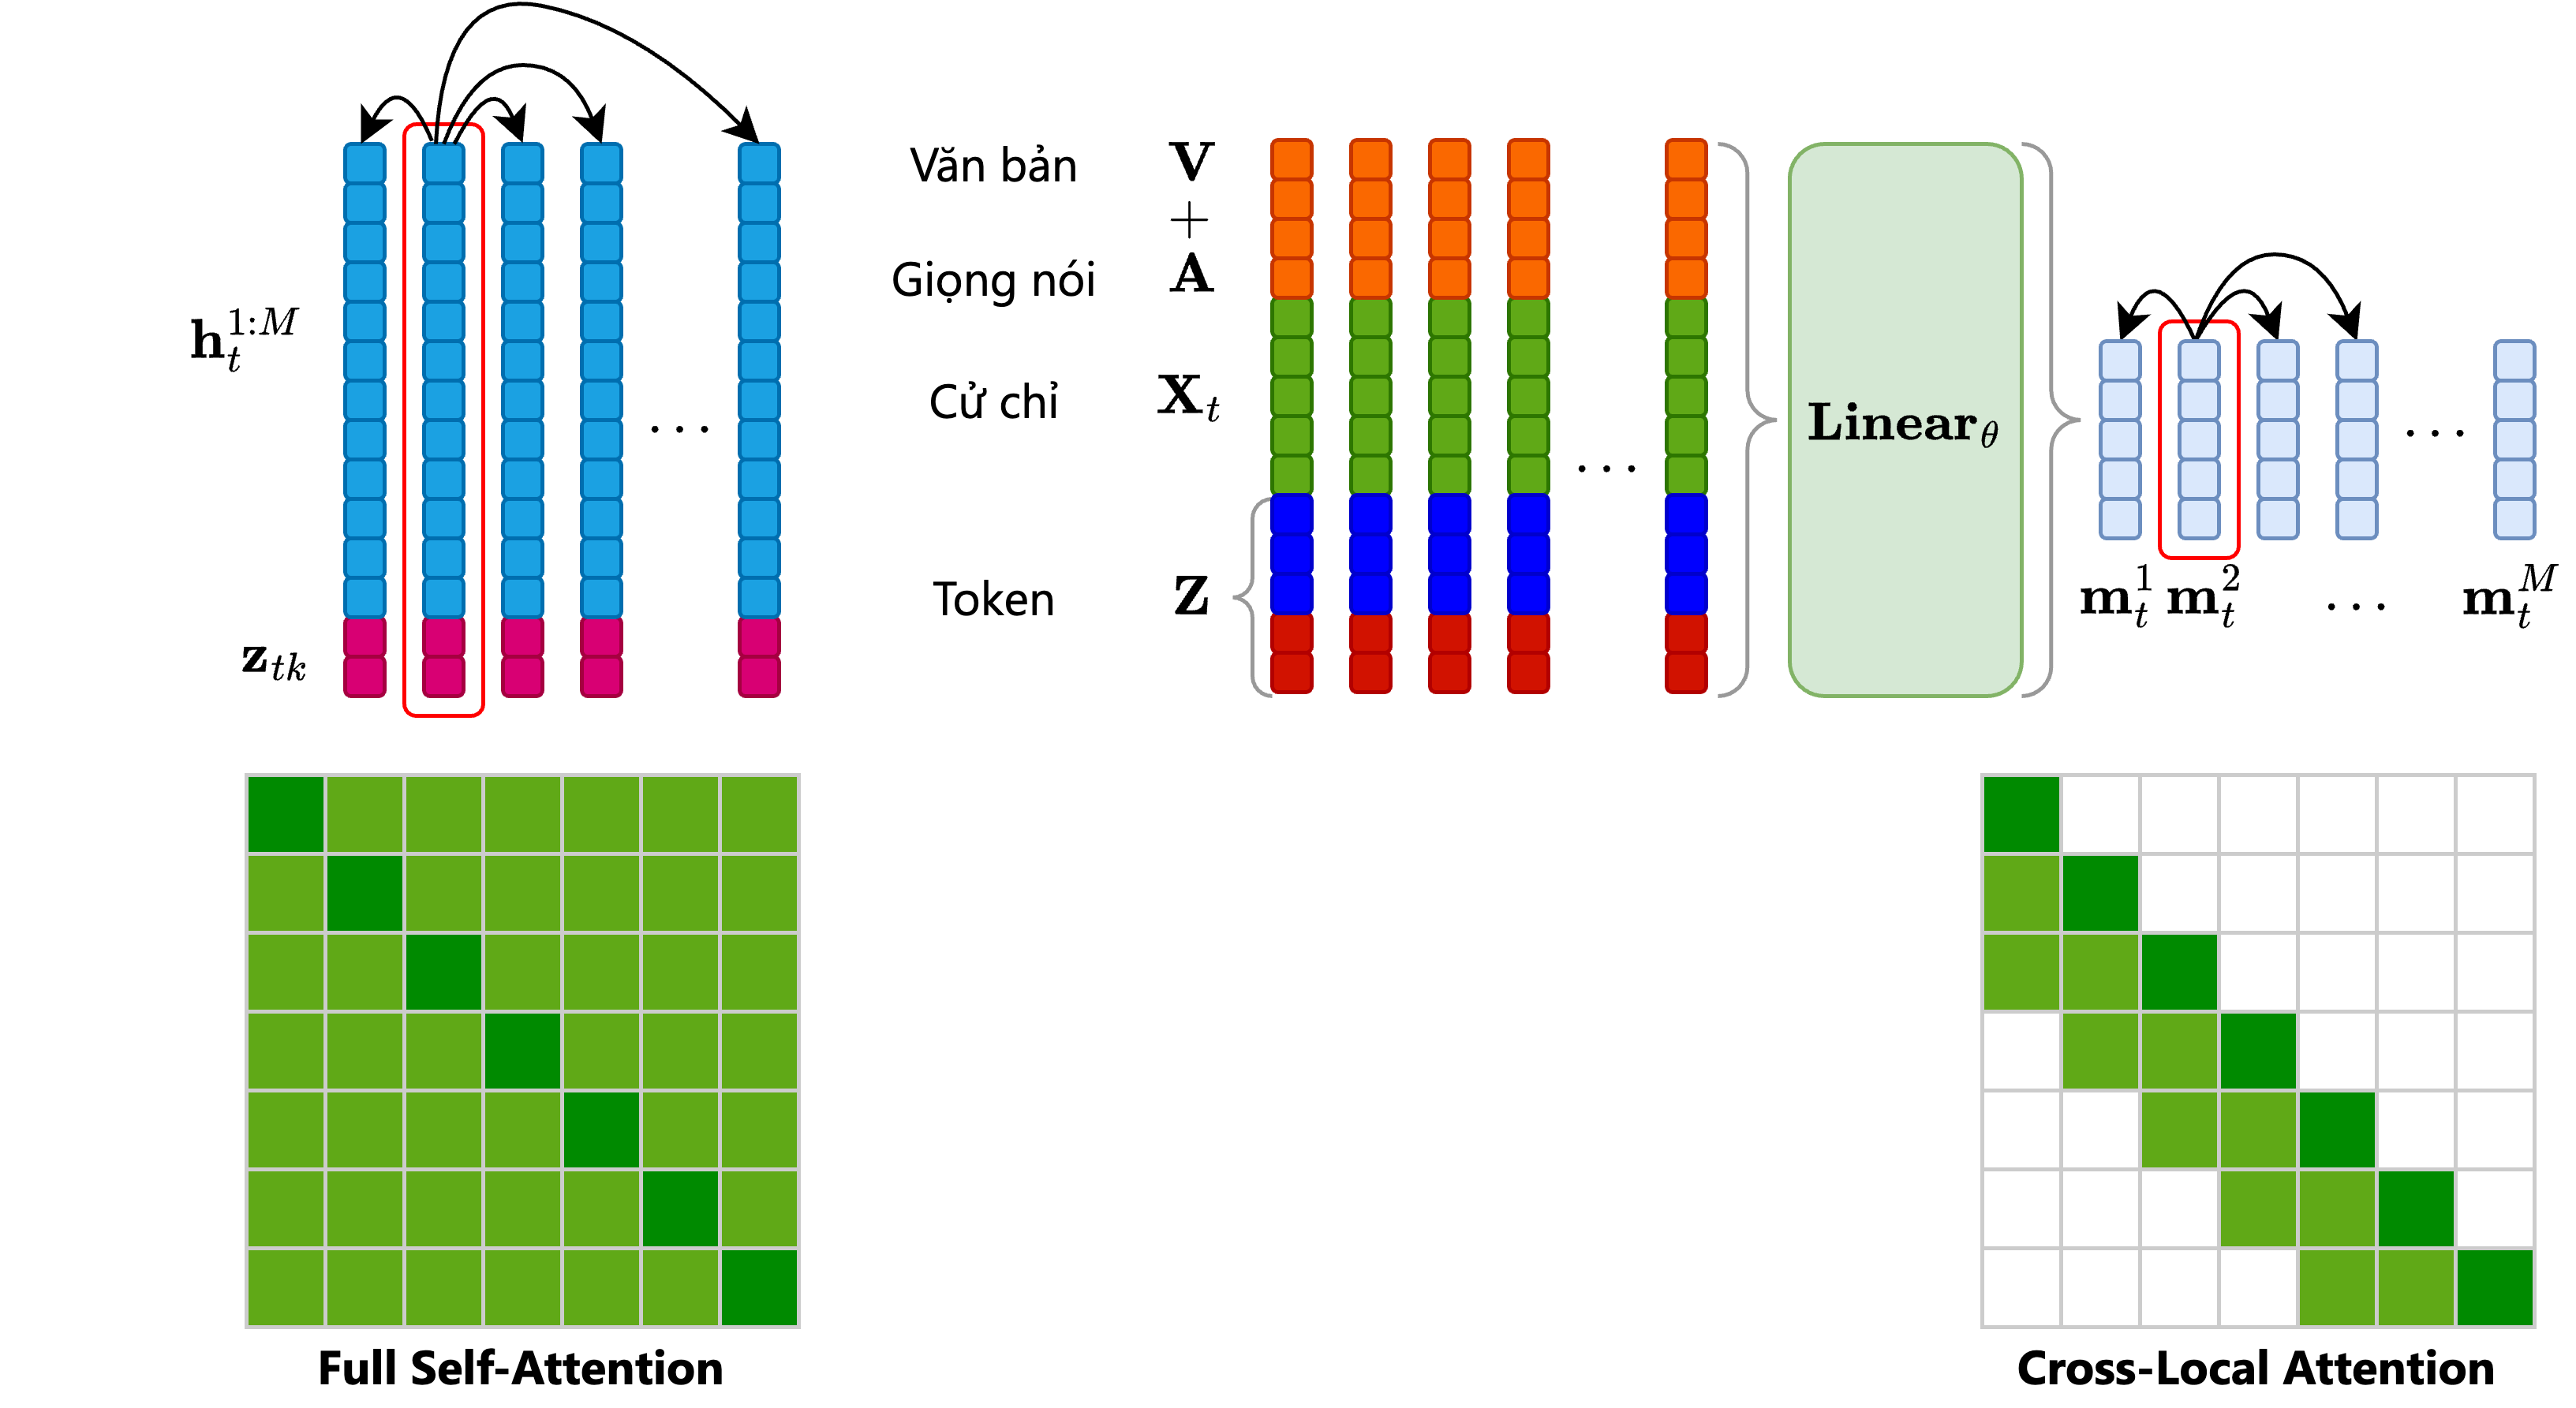
\includegraphics[width=1\textwidth]{CrossLocalAttention}
	\caption{Attention Mechanism in Transformer Encoder and Cross-Local Attention}
	\label{fig:CrossLocalAttention}
\end{figure}

The Attention mechanism functions like a dictionary, where the final retrieved information is the matrix $\mathbf{V}$ (value), while $\mathbf{Q}$ (query) represents the keyword being searched for, and $\mathbf{K}$ (key) is the set of keywords in the lookup dictionary. The Attention process computes the similarity between \( \mathbf{Q} \) and \( \mathbf{K} \) to determine the weights for the values in \( \mathbf{V} \).

The final result is a weighted combination of the values in \( \mathbf{V} \), where the values corresponding to keys most similar to the query receive higher weights. $\mathbf{M}$ is the mask used to perform local attention. The Cross-Local Attention mechanism is illustrated on the right in \autoref{fig:CrossLocalAttention}, while the Transformer Encoder layer uses Self-Attention shown on the left.

\subsubsection{Combining Local Features with Cross-Local Attention}

%The matrix $\mathbf{m}_{t} \in \mathbb{R}^{1:M \times 256}$ is then passed through the Cross-Local Attention layer to compute the correlation between local features.

The matrix $\mathbf{m}_{t} \in \mathbb{R}^{1:M \times 256}$ is then passed through the Cross-Local Attention layer to compute the correlations between local features.
% resulting in the matrix $\mathbf{h}_t \in \mathbb{R}^{1:M \times D}$ :


\begin{equation}
	\mathbf{h}_{t}  = \operatorname{Linear}_{\theta}  ( \operatorname{Cross-Local\ Attention}( \mathbf{m}_{t}) )
	\label{eq:CrossLocalAttention}
\end{equation}


% (\operatorname{Query}) (\operatorname{Key}) (\operatorname{Value})
Cross-local Attention is performed with $\mathbf{Q} = \mathbf{K} = \mathbf{V} = \mathbf{m}_{t}$.
Following the idea of the Routing Transformer method \cite{roy2021efficient}, Cross-local Attention highlights the importance of constructing intermediate feature-vector representations before passing them through the Transformer Encoder layer, as shown in \autoref{fig:OHGesture}.
The feature vectors are augmented with a relative position-encoding vector \textbf{RPE} (\textbf{R}elative \textbf{P}osition \textbf{E}ncoding) to preserve temporal ordering before entering the Cross-Local Attention layer.

After Cross-Local Attention, the model is forwarded through a linear layer, as in \autoref{eq:CrossLocalAttention}, to align with the $M$ frames and obtain the matrix $\mathbf{h}_t \in \mathbb{R}^{1:M \times D}$.

\subsubsection{Global Feature Fusion with the Transformer Encoder}

\begin{figure}[h]
	\centering
	\begin{subfigure}{0.42\textwidth}
		\centering
		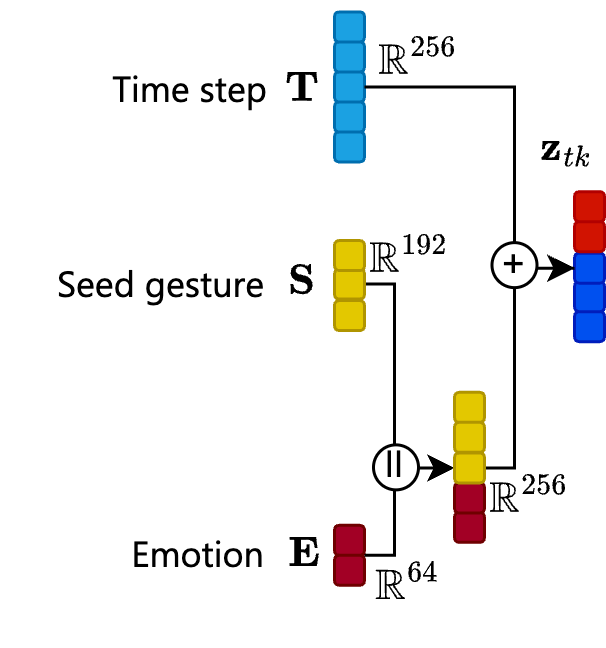
\includegraphics[width=0.9\textwidth]{FeatureConcatenate}
		\caption{Feature concatenation for $\mathbf{z}_{tk}$}
		\label{fig:FeatureFusion}
	\end{subfigure}
	\hfill
	\begin{subfigure}{0.55\textwidth}
		\centering
		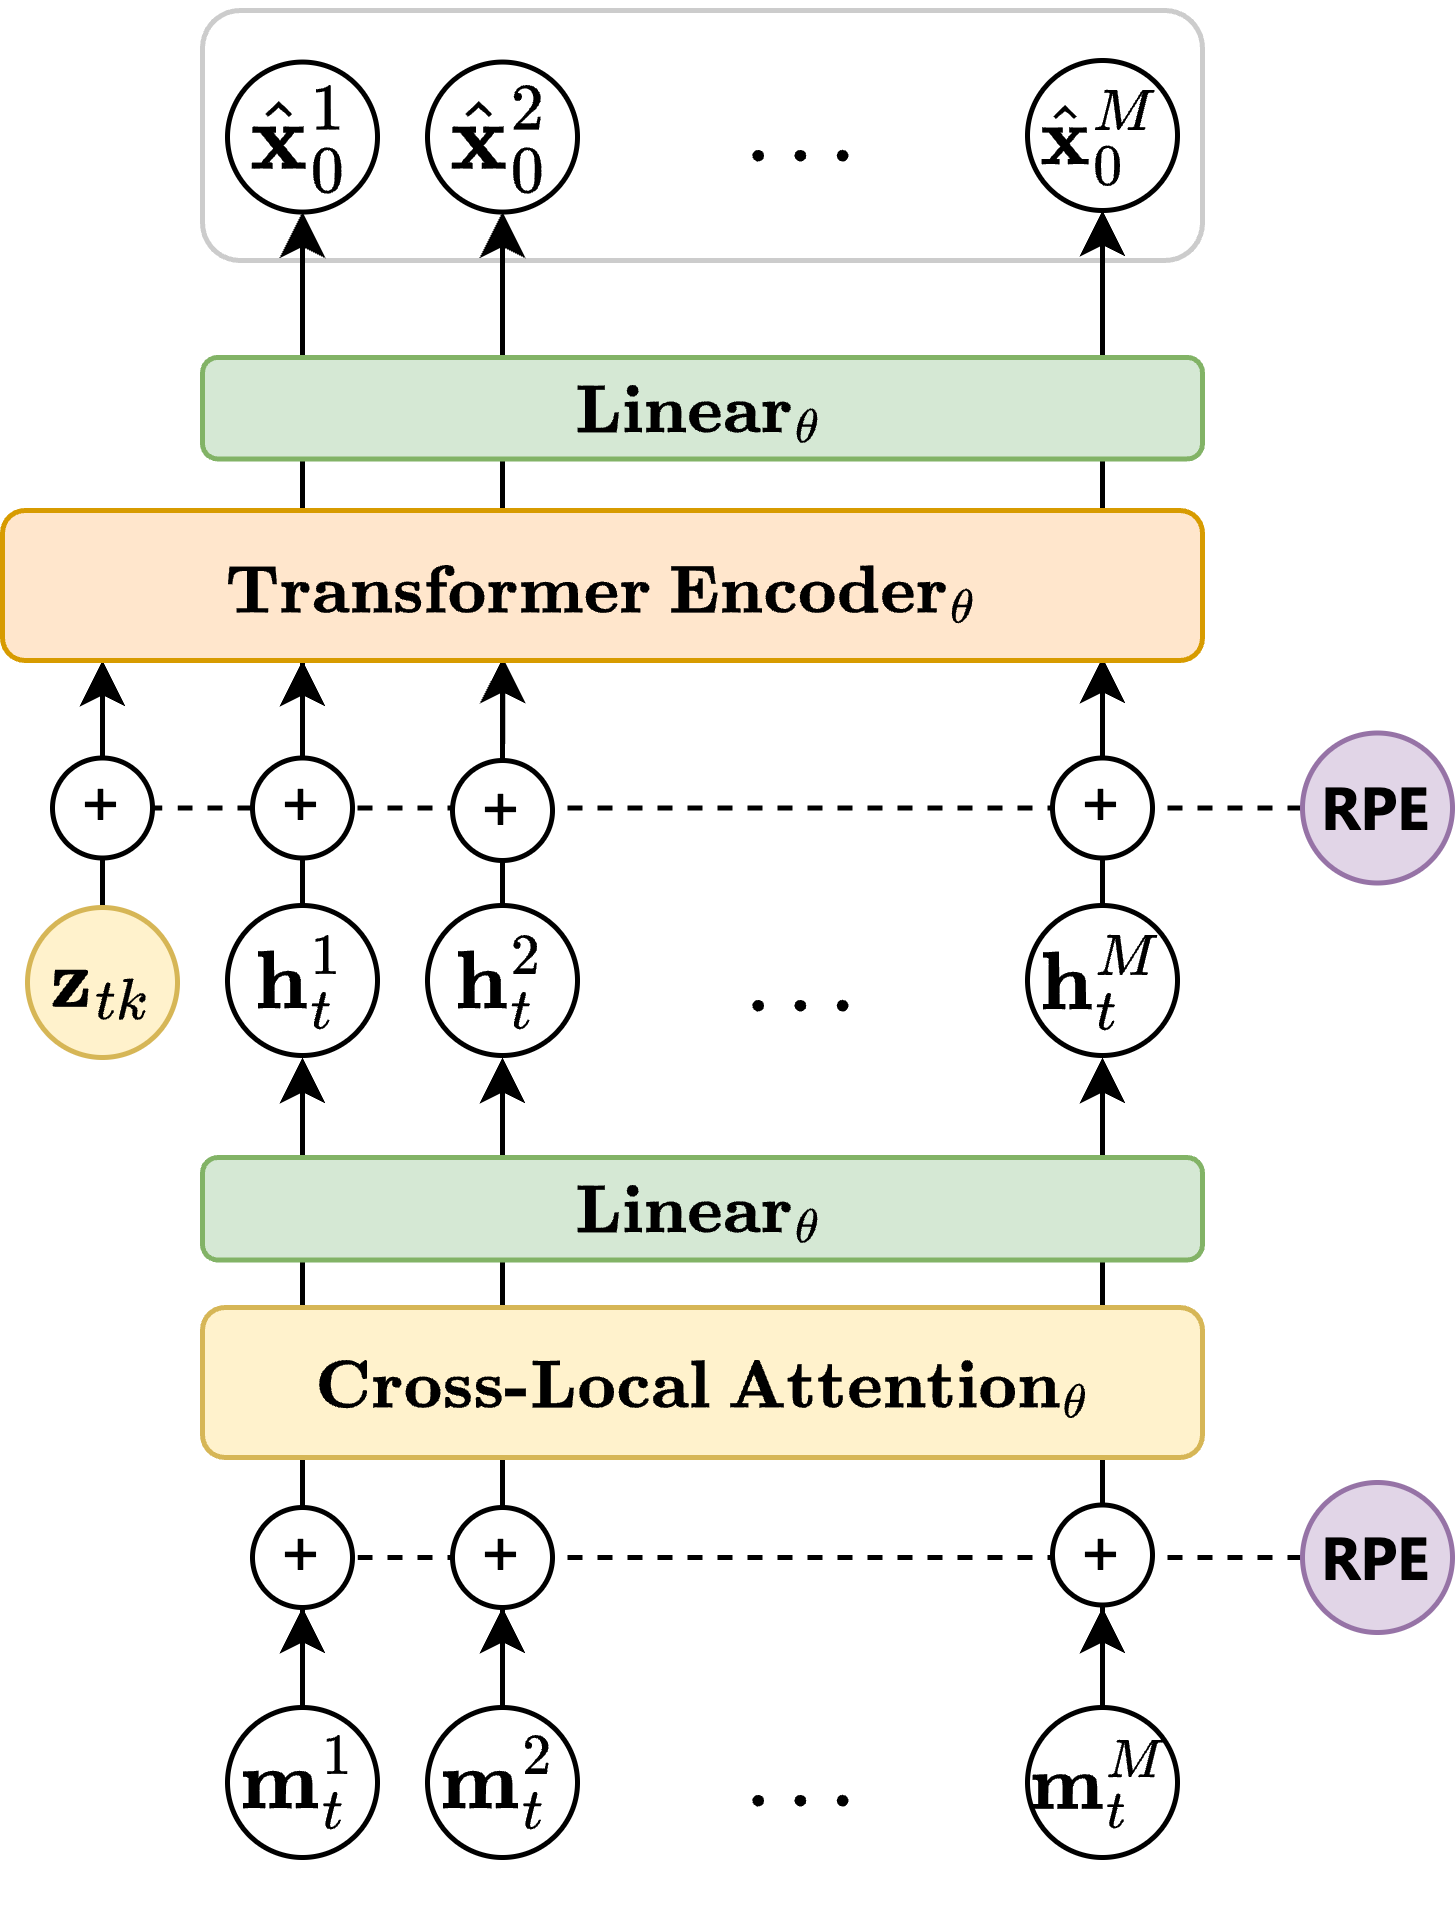
\includegraphics[width=0.85\textwidth]{FeatureFusion}
		\caption{Frame-wise feature-fusion process}
		\label{fig:ZToken}
	\end{subfigure}
\end{figure}

Following MDM \cite{tevet2022human}, the vector $\mathbf{z}_{tk}$ is the first token that encodes information for the entire frame sequence, analogous to the $\texttt{CLS}$ token in BERT \cite{devlin2019bertpretrainingdeepbidirectional}, which summarizes an entire text segment.
Here, the thesis uses $\mathbf{z}_{tk}$, with $\mathbf{z}_{tk} \in \mathbb{R}^{256}$ (\autoref{eq:ConditionConcat}), as the first token representing global features for the whole sequence of $M$ frames.

\begin{equation}
	\mathbf{X}_{0} = \operatorname{Transformer\ Encoder}\bigl(\operatorname{concat}(\mathbf{z}_{tk} \;\|\; \mathbf{h}^{1:M}_{t})\bigr)
	\label{eq:TransformerEncoder}
\end{equation}

The vectors $\mathbf{h}_t$ represent the sequence of $M$ frames. Similar to Reformer \cite{kitaev2020reformer}, before entering the Self-Attention layer of the Transformer Encoder, the model employs Relative Position Encoding (RPE) instead of absolute position encoding, improving efficiency on long sequences.
Within the Transformer Encoder layer \cite{vaswani2017attention}, relationships among the data sequences are computed.
The Transformer Encoder applies the same self-attention mechanism as in \autoref{eq:attention} but without the $\mathbf{Mask}$, enabling correlations across the entire sequence to be captured.

\subsection{Feature Decoding Stage}

In stage \textit{6. Feature Decoding} (\autoref{fig:CommonStage}), once feature correlations are computed, the goal is to upsample the data back to its original dimensionality.

As illustrated in \autoref{fig:OHGesture}, the latent matrix $\mathbf{X}_{0}$, after passing through the Transformer Encoder to capture correlations among heterogeneous data types, is fed into a linear projection layer
$\hat{\mathbf{x}}_{0} = \operatorname{Linear}_{\theta}(\mathbf{X}_{0})$
to restore the latent matrix to its original size, yielding $\hat{\mathbf{x}}_{0} \in \mathbb{R}^{1:M \times D}$.

The final rendering step is presented in \autoref{sec:Render}.

\subsection{Emotion Control in Gesture Generation}

The preceding steps enable the model to learn gesture generation. To incorporate emotions across different contexts, each emotion is parameterized and varied so that the predictions faithfully express the designated affect.

Analogous to conditional denoising models \cite{ho2022classifier, tevet2022human}, the thesis uses the condition vector
$c = [\mathbf{s}, \mathbf{e}, \mathbf{a}, \mathbf{v}]$,  
where $\mathbf{s}$ is the seed gesture, $\mathbf{e}$ the emotion, $\mathbf{a}$ the associated speech, and $\mathbf{v}$ the text.
The conditional diffusion model injects $c$ at every timestep $t$ in the denoising network $\text{G}_\theta(\bx_{t}, t, c)$, with
$c_{\varnothing} = [\varnothing, \varnothing, \mathbf{a}, \mathbf{v}]$ (unconditional)
and $c = [\mathbf{s}, \mathbf{e}, \mathbf{a}, \mathbf{v}]$ (conditional).
A random mask applied to the seed-gesture and emotion vectors conveniently switches labels, allowing optimization under diverse conditions.

\begin{equation} \label{eq:denoise}
\hat{\bx}_{0\,c,c_{\varnothing},\gamma}
    = \gamma\, G(\bx_{t}, t, c) + (1-\gamma)\, G(\bx_{t}, t, c_{\varnothing})
\end{equation}

Classifier-free guidance \cite{ho2022classifier} further enables interpolation between two emotions
$\mathbf{e}_1$ and $\mathbf{e}_2$ by setting
$c = [\mathbf{s}, \mathbf{e}_{1}, \mathbf{a}, \mathbf{v}]$ and
$c_{\varnothing} = [\mathbf{s}, \mathbf{e}_{2}, \mathbf{a}, \mathbf{v}]$:
\[
\hat{x}_{0\,\gamma, c_{1}, c_{2}}
    = \gamma\, G(x_{t}, t, c_{1}) + (1-\gamma)\, G(x_{t}, t, c_{2}).
\]

\subsection{Training Procedure}

\begin{algorithm}[h]
	\caption{Training in OHGesture}
	\label{alg:trainingohgesture}
	\setlength{\baselineskip}{10pt}
	\begin{enumerate}
		\item Pre-compute $\gamma$, $\sqrt{\alpha_t}$, $\sqrt{1-\alpha_t}$, $\sqrt{\bar{\alpha}_t}$, and random noise $\boldsymbol{\epsilon}_t$ for each timestep $t: 1 \rightarrow T$. Define the noise schedule $\{\alpha_t \in (0,1)\}_{t=1}^T$.
		\item Sample the initial label $\mathbf{x}_0$ from the normalized data distribution.
		\item Randomly generate Bernoulli masks
		      $c_{1} = [ \mathbf{s}, \mathbf{e_1}, \mathbf{a}, \mathbf{v} ]$,
		      $c_{2} = [ \mathbf{s}, \mathbf{e_2}, \mathbf{a}, \mathbf{v} ]$, or
		      $c_{2} = [ \varnothing, \varnothing, \mathbf{a}, \mathbf{v} ]$.
		\item Add noise to obtain the noisy gesture $\mathbf{x}_t$:
		      \[
		      \mathbf{x}_t = \sqrt{\bar{\alpha}_t}\,\mathbf{x}_0 + \sqrt{1-\bar{\alpha}_t}\,\boldsymbol{\epsilon}_t.
		      \]
		\item Sample $t$ \textbf{uniformly} from $[1, T]$.
		\item Given $\mathbf{x}_t$, $t$, and masks $c_1$, $c_2$, predict the gesture sequence:
		      \[
		      \hat{\mathbf{x}}_{0\,\gamma,c_{1},c_{2}}
		          = \gamma\, G_{\theta}(\mathbf{x}_{t}, t, c_{1})
		          + (1-\gamma)\, G_{\theta}(\mathbf{x}_{t}, t, c_{2}).
		      \]
		\item Compute the loss and gradient to update $\theta$:
		      \[
		      \mathcal{L}^t
		          = \mathbb{E}_{t, \mathbf{x}_0, \boldsymbol{\epsilon}_t}
		            \bigl[\operatorname{HuberLoss}(\mathbf{x}_0, \hat{\mathbf{x}}_0)\bigr].
		      \]
		\item Repeat from step 6 until convergence, obtaining the optimal parameters $\theta'$.
	\end{enumerate}
\end{algorithm}

\autoref{alg:trainingohgesture} trains the OHGesture model by first computing the required values and hyper-parameters—$\gamma$, $\sqrt{\alpha_t}$, $\sqrt{1-\alpha_t}$, $\sqrt{\bar{\alpha}_t}$, and $\boldsymbol{\epsilon}_t$—for every timestep $t$ (1 … $T$).  
The initial label $\mathbf{x}_0$, representing the ground-truth gesture, is drawn from the normalized data distribution.  
Random Bernoulli masks $c_1$ and $c_2$ emulate different conditions (gesture, emotion, speech, or text), with one mask possibly lacking emotion information.  
Noise is then added to create the noisy gesture $\mathbf{x}_t$.  
A timestep $t$ is sampled uniformly, and $\mathbf{x}_t$ with the masks is fed into the model to predict the original gesture sequence as a weighted combination of conditional outputs.  
The Huber loss between ground-truth and prediction is used to update $\theta$.  
This cycle repeats until the model converges, yielding the optimal parameters $\theta'$.

\subsection{Sampling Process}

\begin{figure}[h]
	\centering
	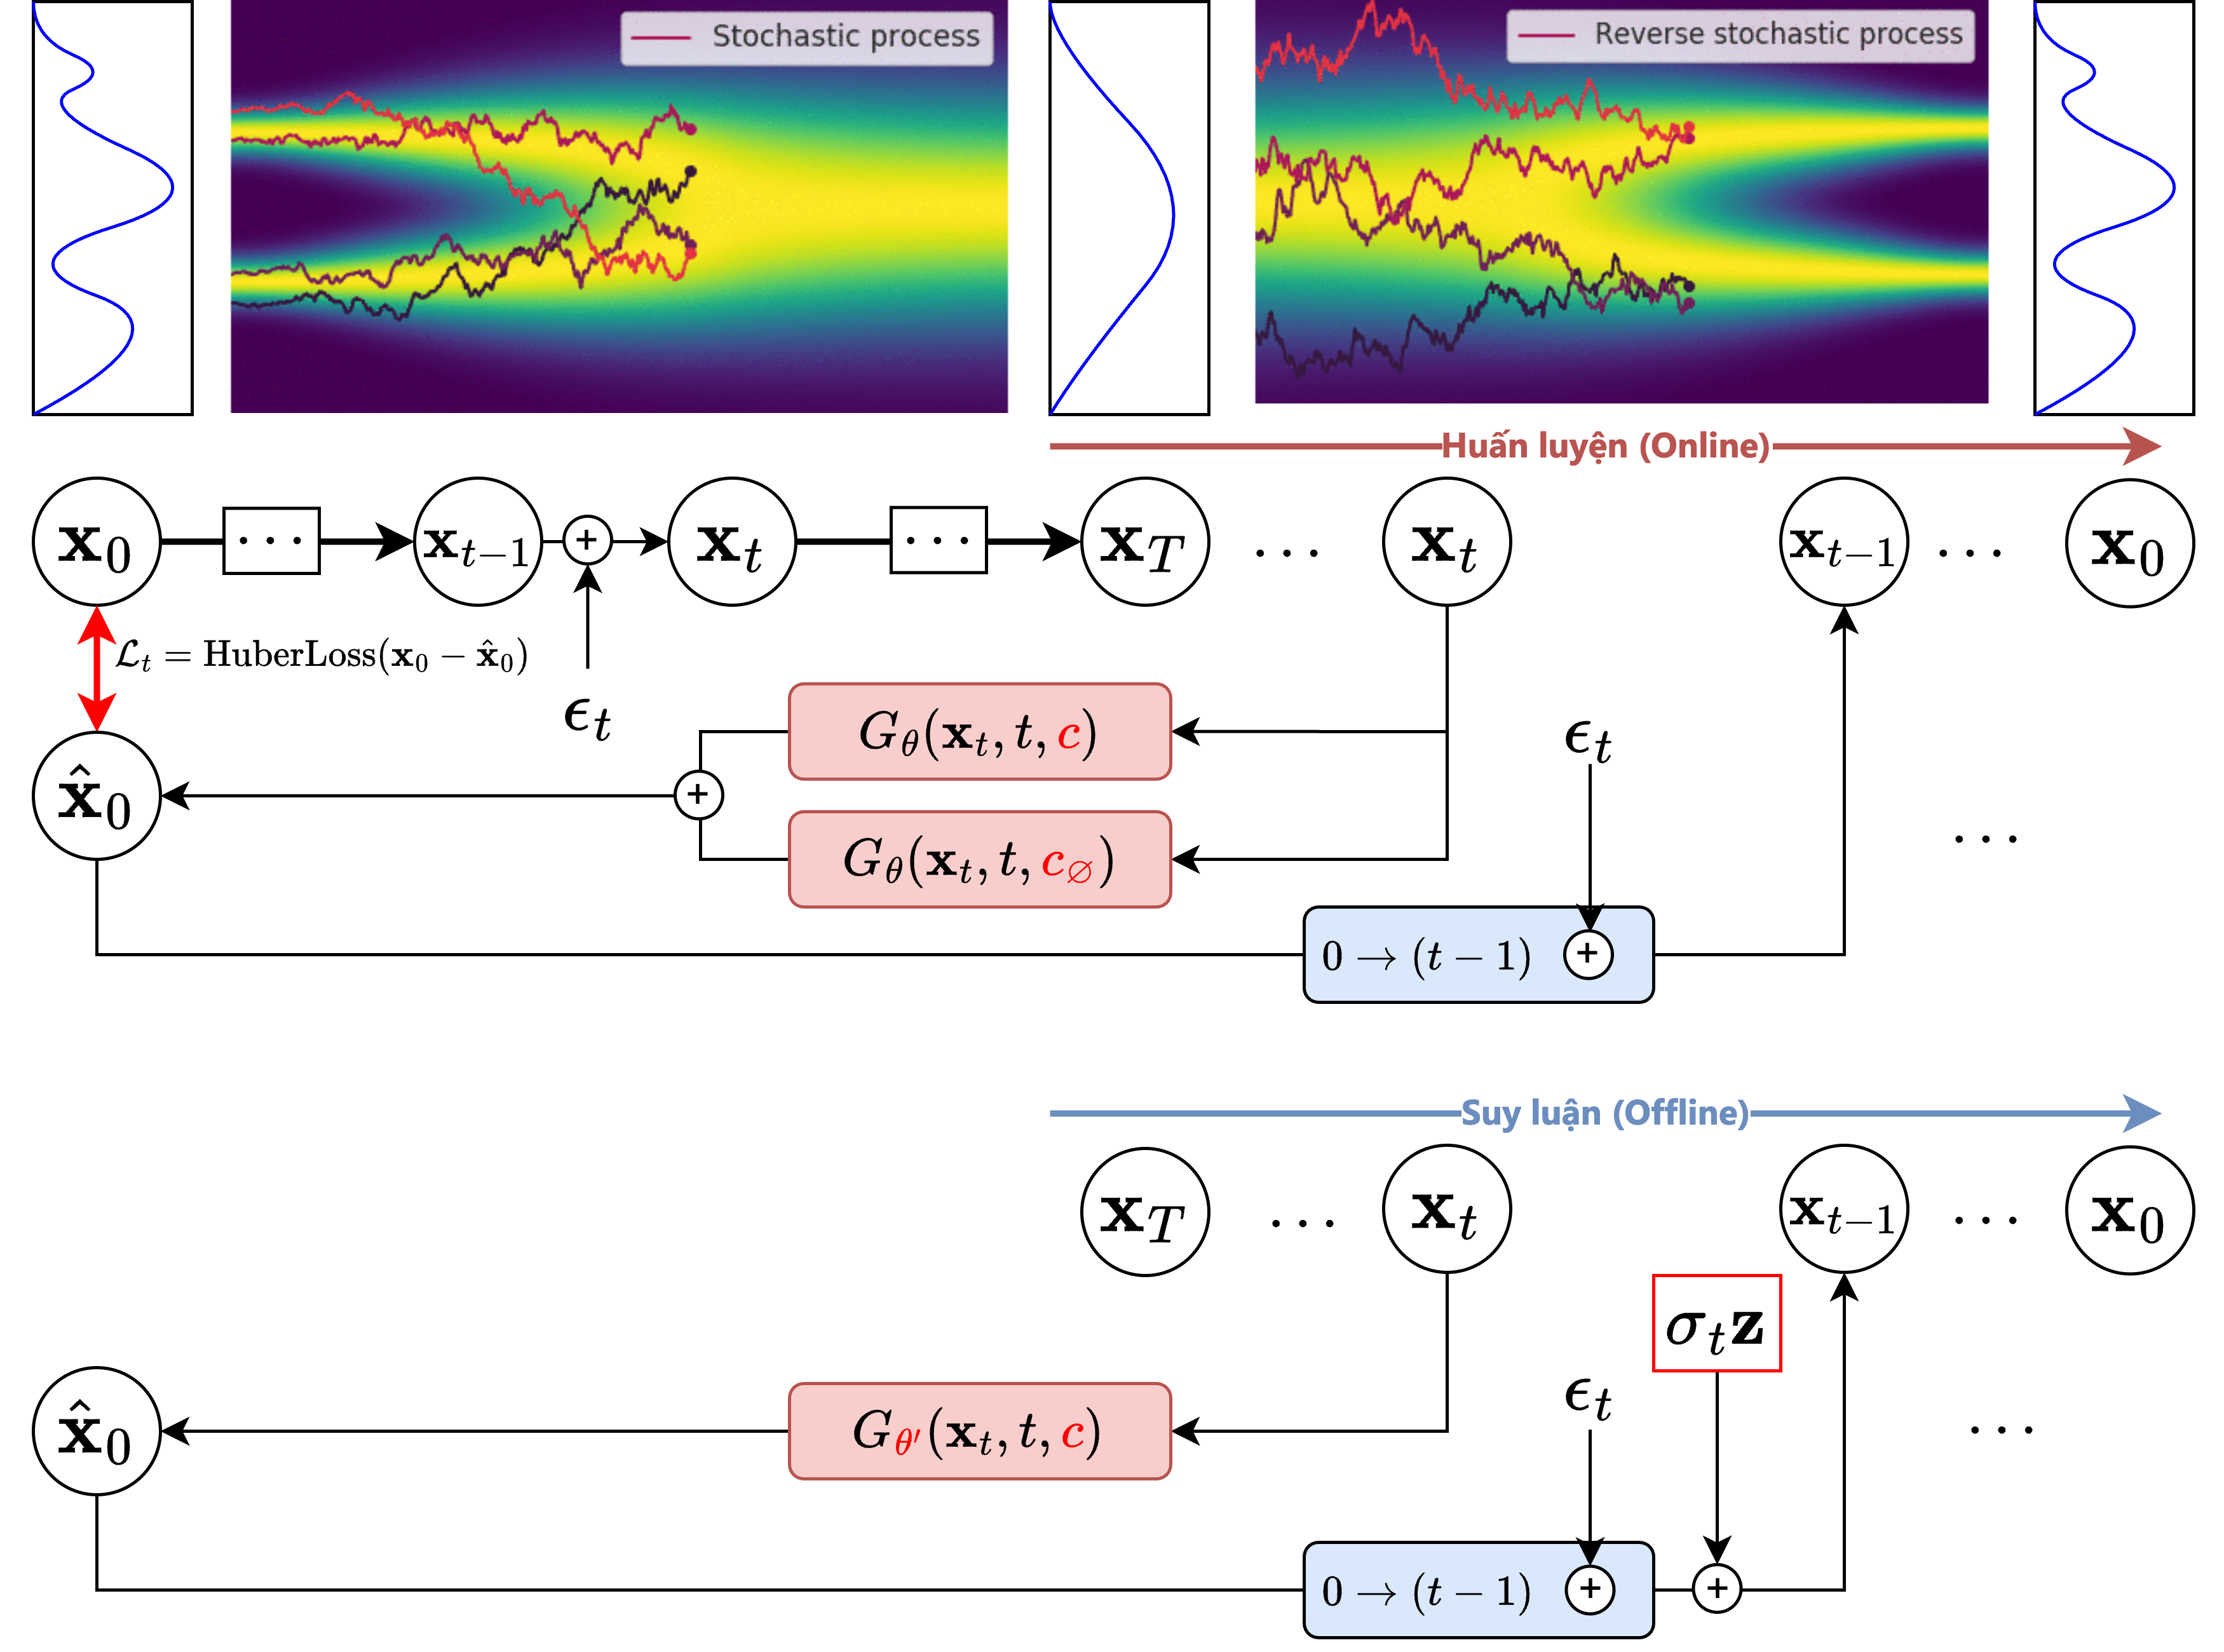
\includegraphics[width=\linewidth]{OnlineAndOffline}
	\caption{Offline (Training) and Online (Inference) Phases}
	\label{fig:OnlineAndOffline}
\end{figure}

To generate gestures of arbitrary length, the original sequence is segmented into clips of length $M$.
During training, the seed gesture can be chosen by randomly selecting a gesture from the dataset or by averaging the clipped segments—here, the mean rotation angles are used.  
Generated frames are processed sequentially, with the last $N=8$ frames taken as the seed for the next iteration.  
For each clip, the gesture $\bx_{t}$ is denoised via $\hat{\bx}_{0} = G_{\theta'}(\bx_{t}, t, c)$; noise is re-added to obtain $\bx_{t-1}$, and the procedure repeats until $t=1$, yielding $\bx_{0}$.

\begin{algorithm}[H]
	\caption{Sampling in OHGesture}
	\label{alg:sampling}
	\setlength{\baselineskip}{10pt}
	\begin{enumerate}
		\item Initialize with noise: $\mathbf{x}_T \sim \mathcal{N}(0, \mathbf{I})$.
		\item Retrieve $\sqrt{\alpha_t}$, $\sqrt{1 - \alpha_t}$, and $\sqrt{\bar{\alpha}_t}$ from training; precompute $\sigma_t$ from $\alpha_t$ for each timestep $t: 1 \rightarrow T$.
		\item Split each 4-second speech segment into $\mathbf{a} \in \mathbb{R}^{64000}$.  
		      The initial seed gesture $\mathbf{s}$ is the data mean and is later updated from the inferred gesture segment.  
		      Select the desired emotion, obtain the transcript $\mathbf{v}$ from speech $\mathbf{a}$, and form the condition $c = [\mathbf{s}, \mathbf{e}, \mathbf{a}, \mathbf{v}]$.
		\item For each timestep, take $t$ \textbf{sequentially} from $[T, \dots, 1]$.
		\item Sample random noise $\mathbf{z} \sim \mathcal{N}(0, \mathbf{I})$.
		\item Infer $\hat{\mathbf{x}}_0^{(t)} = G_{\theta'}(\mathbf{x}_t, t, c)$.
		\item Diffuse $\hat{\mathbf{x}}_0^{(t)}$ from step $0 \rightarrow t$ to obtain $\hat{\mathbf{x}}_{t-1}^{(t)}$.
		\item Add noise: $\hat{\mathbf{x}}_{t-1} = \hat{\mathbf{x}}_{t-1}^{(t)} + \sigma_t \mathbf{z}$.
		\item Return to step 4.  
		      When $t = 1$, output the denoised gesture $\hat{\mathbf{x}}_0$.
	\end{enumerate}
\end{algorithm}

\autoref{alg:sampling} starts by initializing the noisy gesture $\mathbf{x}_T$ from $\mathcal{N}(0, \mathbf{I})$.  
The values $\sqrt{\alpha_t}$, $\sqrt{1-\alpha_t}$, and $\sqrt{\bar{\alpha}_t}$ obtained during training, together with $\sigma_t$, are employed at each timestep (1 … $T$).  
Each 4-second speech segment is represented by $\mathbf{a}$, and the seed gesture $\mathbf{s}$ is taken as the data mean or from the previously inferred segment.  
The desired emotion and the transcript form the condition $c = [\mathbf{s}, \mathbf{e}, \mathbf{a}, \mathbf{v}]$.  
The algorithm proceeds sequentially from $T$ to 1: random noise $\mathbf{z}$ is generated, the model predicts $\hat{\mathbf{x}}_0^{(t)}$ from $\mathbf{x}_t$, $t$, and $c$, then $\hat{\mathbf{x}}_{t-1}^{(t)}$ is computed and updated with noise.  
This loop continues until $t=1$, after which the algorithm outputs the final denoised gesture $\hat{\mathbf{x}}_0$.

%
%\chapter{EXPERIMENTS}
\label{Chapter4}

\section{Dataset}

\begin{figure}[h]
	\centering
	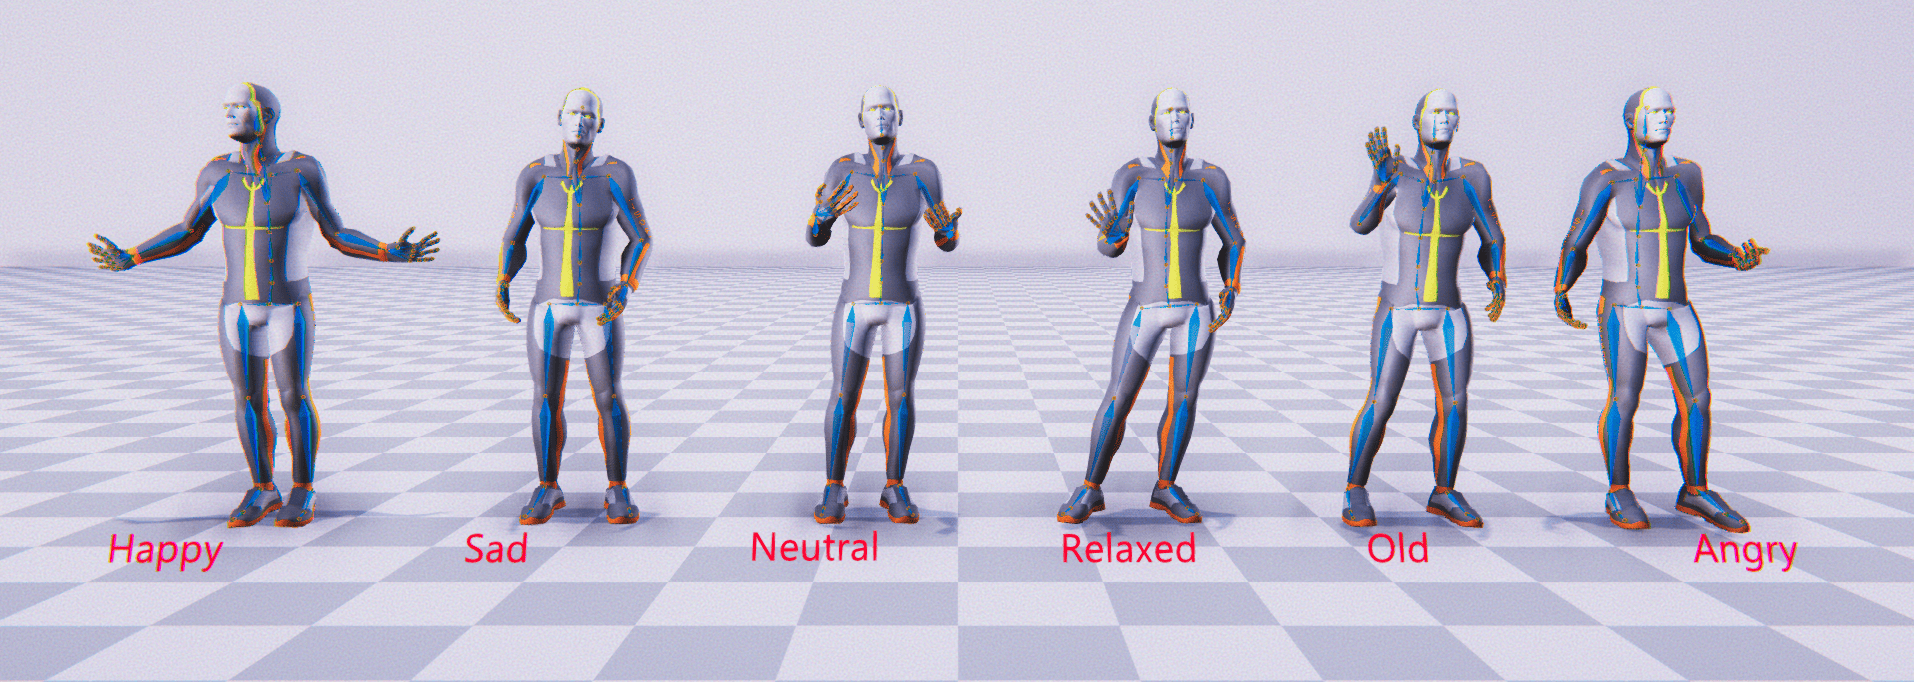
\includegraphics[width=\textwidth]{EmotionAnimation}
	\caption{Illustration of 6 gestures: $\texttt{Happy}$, $\texttt{Sad}$, $\texttt{Neutral}$, $\texttt{Old}$, $\texttt{Relaxed}$, and $\texttt{Angry}$}
\end{figure}

This thesis uses the ZeroEGGS dataset \cite{ghorbani2022zeroeggszeroshotexamplebasedgesture}, a motion capture dataset designed for research and development of gesture generation models. It includes 67 monologue clips performed by a female motion capture actor, with a total duration of 135 minutes. The monologues are annotated with 6 different emotions: $\texttt{Happy}$, $\texttt{Sad}$, $\texttt{Neutral}$, $\texttt{Old}$, $\texttt{Relaxed}$, and $\texttt{Angry}$, enabling simulation of various emotional states in gestures and body movements. ZeroEGGS provides a rich platform for studying the integration of speech and dynamic gestures, supporting the development of models capable of adapting gestures according to emotions and text semantics.

\section{Data Preprocessing}
\label{sec:Preprocessing}

In stage {1. Data Preprocessing} (\autoref{fig:CommonStage}), gesture, speech, and text data are read and processed to be represented as vectors or matrices containing information derived from raw data.

For \textbf{text data}: the thesis uses the $\texttt{nltk}$ library for tokenization and $\texttt{contractions}$ to normalize contracted words.

One contribution of the thesis is to convert the speech data available in ZeroEGGS using Adobe Speech To Text, then align the phonetic timestamps using the Montreal Forced Aligner \cite{saxon2020robust} with an English phoneme dictionary to match the gesture frame rate, generating TextGrid files. From these TextGrids containing word-level timing information, the thesis uses $\texttt{gensim}$ to generate word2vec embeddings.

\textbf{Gesture data} consists of BVH (BioVision Motion Capture) files captured via motion capture systems. BVH files include two components: Hierarchy and Motion. Specifically:

\begin{itemize}
	\item \texttt{HIERARCHY}: defines a skeletal tree containing 75 bones $\{ \mathbf{b}_1, \mathbf{b}_2 \cdots \mathbf{b}_{75} \}$, each with an initial position (\texttt{OFFSET}) and \texttt{CHANNELS} parameters specifying the type and order of rotation angles (\texttt{Zrotation}, \texttt{Yrotation}, \texttt{Xrotation}) and position (\texttt{Xposition}, \texttt{Yposition}, \texttt{Zposition}), which are defined in the \texttt{MOTION} section. The first bone (usually \texttt{Hips}) is the root bone $\mathbf{b}_{\text{root}}$, used to define the T-pose via forward kinematics as the initial pose of the skeleton before applying motion.
	
	\item \texttt{MOTION}: a sequence of frames, each containing motion data representing changes of all $75$ bones as defined by the \texttt{CHANNELS} in the \texttt{HIERARCHY}.
\end{itemize}

The model in the thesis converts Euler rotation angles to quaternion rotation angles, where a quaternion is a 4-dimensional vector.

\begin{equation} \label{eq:gesturevector}
	\mathbf{g} = \Big[ \mathbf{p}_{\text{root}},  \mathbf{r}_{\text{root}},
	\mathbf{ p }'_{\text{root}},  \mathbf{r}'_{\text{root}},
	\mathbf{p}_{\text{joins}},  \mathbf{r}_{\text{joins}},
	\mathbf{p}'_{\text{joins}},  \mathbf{r}'_{\text{joins}},
	\mathbf{d}_{\text{gaze}}
	\Big]
\end{equation}

Here, each $\mathbf{g} \in \mathbb{R}^{1141}$ includes:
{
	\begin{itemize}
		\item $\mathbf{p}_{\text{root}} \in \mathbb{R}^3$: coordinates of the root joint
		\item $\mathbf{r}_{\text{root}} \in \mathbb{R}^4$: rotation (quaternion) of the root joint
		\item $\mathbf{p}'_{\text{root}} \in \mathbb{R}^3$: velocity of the root position
		\item $\mathbf{r}'_{\text{root}} \in \mathbb{R}^3$: angular velocity of the root rotation
		
		\item $\mathbf{p}_{\text{joins}} \in \mathbb{R}^{3 n_{\text{join} }}$: positions of other joints
		\item $\mathbf{r}_{\text{joins}} \in \mathbb{R}^{6 n_{\text{join} }}$: joint rotations on the X and Y planes
		\item $\mathbf{p}'_{\text{joins}} \in \mathbb{R}^{3n_{\text{join} }}$: velocity of joint positions
		\item $\mathbf{r}'_{\text{joins}} \in \mathbb{R}^{3n_{\text{join} }}$: angular velocity of joint rotations
		\item $\mathbf{d}_{\text{gaze}} \in \mathbb{R}^3$: gaze direction
\end{itemize}}

The original gesture sequences in Euler angles are converted to radians, then converted from Euler to Quaternion as detailed in \autoref{appendix:BVHData:QuaternionConvert}.

\textbf{Speech data}: $\mathbf{a}_{\text{raw}} \in \mathbb{R}^{ \text{length } }$ is raw speech sampled at 16000 Hz, trimmed into segments $\mathbf{a} \in \mathbb{R}^{64000}$ corresponding to 4 seconds. The thesis uses \texttt{ffmpeg-normalize} to normalize volume to a level lower than the original.

\textbf{Emotion}: Emotion data is represented using a predefined one-hot encoded vector. During sampling, the filename encodes the target emotion.

All data is stored using the $\texttt{h5}$ format.

\section{Training Process}

The entire model training process was conducted over approximately two weeks with the following parameters: number of training steps $T = 1000$, using an Nvidia 3090 GPU. The learning rate was set to $3 \times 10^{-5}$, batch size was $640$, and a total of $43,853$ samples were trained. At each step, $t$ is randomly sampled and input to $f_{\theta}$ to predict $\mathbf{x}_{0}$. The emotional control parameter was set to $\gamma = 0.1$. The probability of applying random masking to the emotion and initial gesture matrices was $10\%$, using a Bernoulli distribution to randomly hide/reveal these matrices.

The $\beta$ parameter was scheduled linearly from $0.5 \rightarrow 0.999$.

The $\operatorname{HuberLoss} (\mathbf{x}_{0},  \hat{\mathbf{x}}_{0} )$ is computed as follows:

\begin{itemize}
\item If $|\mathbf{x}_0 - \hat{\mathbf{x}}_0| \leq \delta$ then $\mathcal{L}_{ \delta, \mathbf{x}_0, \hat{\mathbf{x}}_0} = \frac{1}{2} (\mathbf{x}_0 - \mathbf{x}_0)^2$: Below the threshold, the loss is computed as squared distance (similar to MSE), which is sensitive to small errors and provides smooth gradients.

\item If $|\mathbf{x}_0 - \hat{\mathbf{x}}_0| > \delta$ then $\mathcal{L}_{ \delta, \mathbf{x}_0, \hat{\mathbf{x}}_0}  =  \delta \cdot |\mathbf{x}_0 - \mathbf{x}_0| - \frac{1}{2} \delta^2$: Above the threshold, the loss behaves like MAE, reducing sensitivity to large errors and improving robustness against outliers.

\end{itemize}

The training process is implemented in the open-source repository: \hyperlink{https://github.com/hmthanh/OHGesture}{Github/OHGesture} \footnote{\url{https://github.com/hmthanh/OHGesture}}.

\section{Rendering Process in Unity}
\label{sec:Render}

To visualize the gesture generation process from model output, the thesis uses Unity in stage \textit{7. Rendering} (\autoref{fig:CommonStage}), extending code from the DeepPhase model \cite{starke2022deepphase}. The generated output is in BVH (BioVision Motion Capture) format. In Unity, the author adds C-Sharp scripts to render gestures based on coordinates and labels, with bone positions and rotations represented using quaternions.

Rendering details are presented in \autoref{Appendix3}.

The Unity project source code is available at: \hyperlink{https://github.com/DeepGesture/deepgesture-unity}{Github/DeepGesture-Unity}
\footnote{\url{https://github.com/DeepGesture/deepgesture-unity}}.

%
%
\chapter{KẾT QUẢ VÀ ĐÁNH GIÁ}
\label{chap:evalution}

\section{Phương pháp đánh giá}

Quá trình đánh giá được thực hiện qua hai độ đo chính là: Mean Opinion Scores (MOS) và Fréchet Inception Distance (FID).

\subsection{Đánh giá dựa trên cảm nhận của con người}

\subsubsection{Mean Opinion Scores (MOS)}

Hiện tại, chưa có một độ đo chung cho bài toán sinh cử chỉ, đặc biệt là sinh cử chỉ từ giọng nói, vì vậy luận văn dựa vào đánh giá chủ quan của con người để thực hiện các đánh giá thực nghiệm. 
Tương tự như các phương pháp trước đây \cite{yoon2022genea}, \cite{kucherenko2021large}, các mô hình sinh cử chỉ điều khiển bằng giọng nói vẫn thiếu các chỉ số mục tiêu phản ánh một cách nhất quán với nhận thức chủ quan của con người  \cite{alexanderson2022listen}.

MOS được đo lường thông qua ba tiêu chí:

\begin{itemize}
	\item Human-likeness (Mức độ giống con người)
	\item Gesture-Speech Appropriateness (Sự phù hợp giữa cử chỉ và giọng nói)
	\item Gesture-style Appropriateness (Sự phù hợp giữa phong cách cử chỉ)
\end{itemize}

Một trong những đóng góp của luận văn là xây dựng  \hyperlink{https://genea-workshop.github.io/leaderboard/}{GENEA Leaderboard} \footnote{  \url{https://genea-workshop.github.io/leaderboard} } \cite{nagy2024towards}. Hệ thống này bao gồm HEMVIP (\textbf{H}uman \textbf{E}valuation of \textbf{M}ultiple \textbf{V}ideos in \textbf{P}arallel) nhằm so sánh kết quả sinh trực quan giữa các video được tạo ra từ kết quả kết xuất.

\begin{figure}[H]
	\centering
	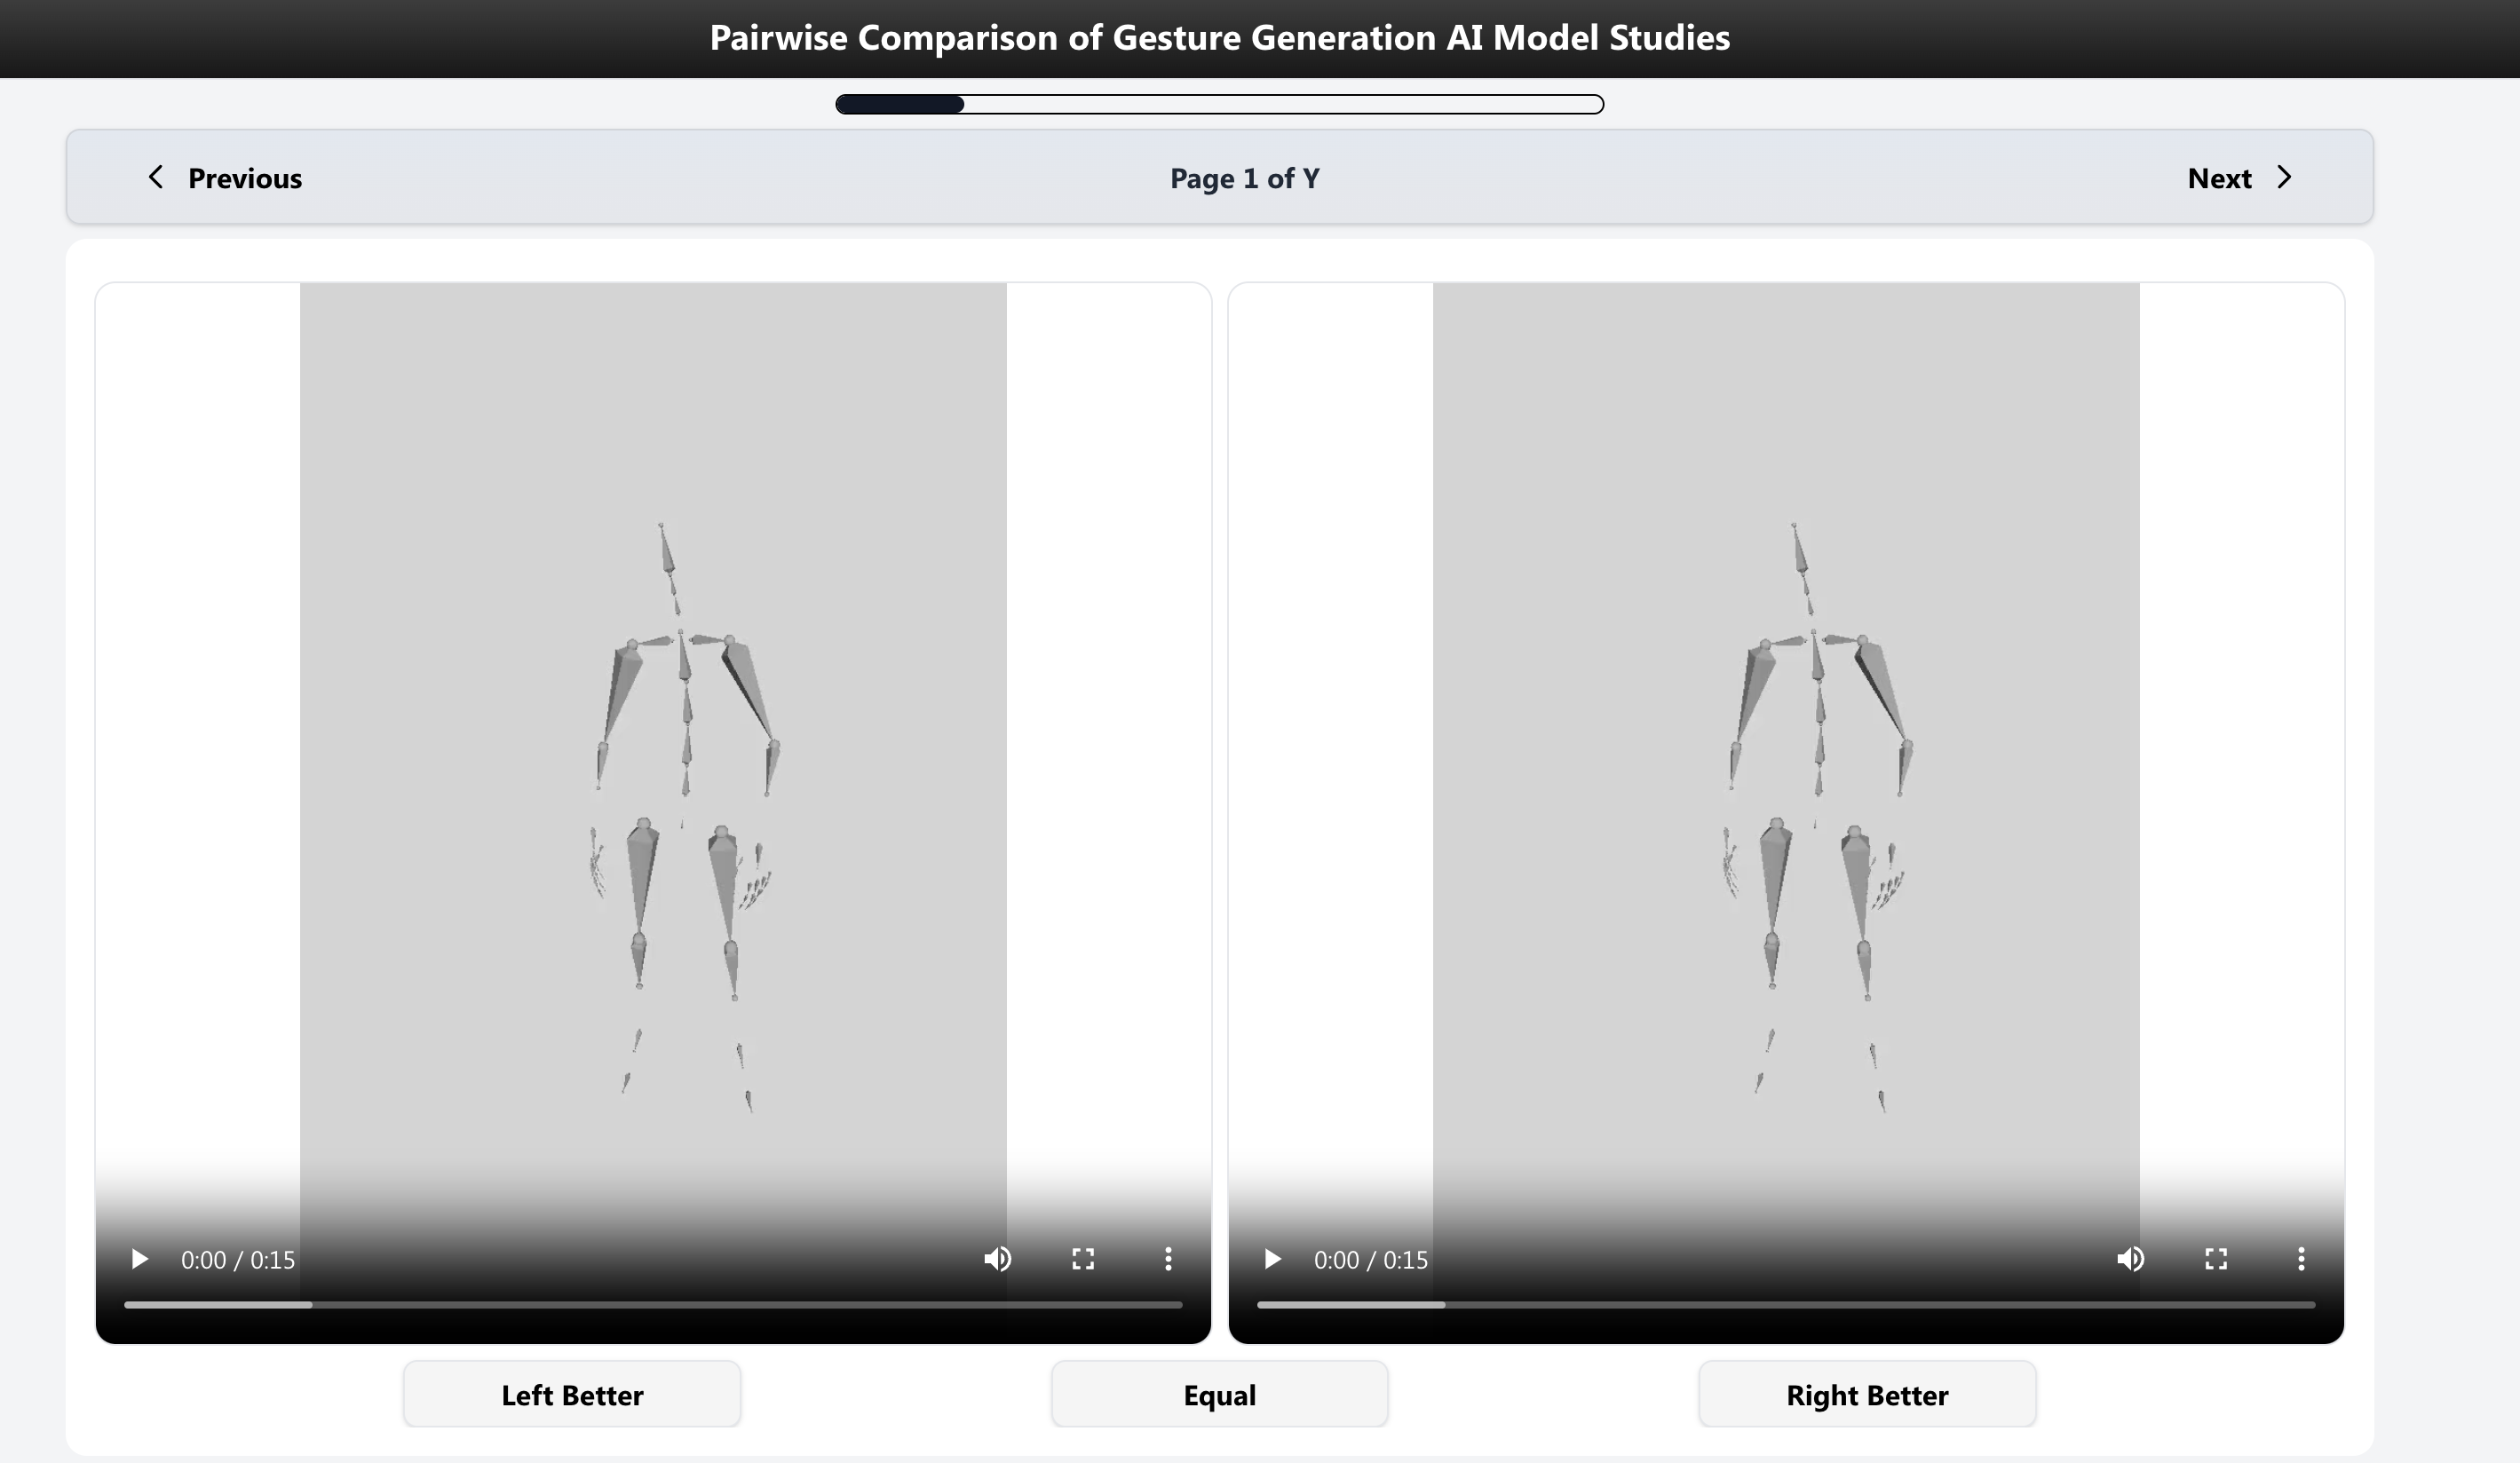
\includegraphics[width=\textwidth]{hemvip}
	\caption{Hệ thống HEMVIP nhằm đánh giá kết quả sau khi kết xuất của hai mô hình}
\end{figure}

Trong nhóm GENEA (\textbf{G}eneration and \textbf{E}valuation of \textbf{N}on-verbal Behaviour for \textbf{E}mbodied \textbf{A}gents), chúng tôi sẽ thuê các người đánh giá trên Prolific và thực hiện nghiên cứu người dùng (User Study) theo kết quả kết xuất trên video, người tham gia sẽ đánh giá \textit{Bên Trái Tốt Hơn} (Left Better), \textit{Bằng Nhau} hoặc \textit{Bên Phải Tốt Hơn} (Right Better). Điểm số sẽ cập nhật sẽ là $-1$, $0$ và $1$ cho mô hình cho các kết quả sinh bao gồm cả dữ liệu thật. Kết quả so sánh của toán bộ mô hình sẽ được cập nhật bằng hệ thống đánh giá Elo (Elo rating system).

Mã nguồn của chương trình được công khai ở \hyperlink{https://github.com/hemvip/hemvip.github.io/}{github.com/hemvip.github.io}
\footnote{HEMVIP 2 \url{https://github.com/hemvip/hemvip.github.io}}.


\subsection{Đánh giá dựa trên các độ đo số học}

\subsubsection{Sai số toàn phương trung bình (Mean Square Error)}

Độ đo sai số toàn phương trung bình giữa chuỗi cử chỉ dự đoán $\hat{\mathbf{y}}_i^{1:M \times D}$ và chuỗi cử chỉ thật $\mathbf{y}_i^{1:M \times D}$ được thực hiện theo công thức sau:

\begin{equation}
\text{MSE} = \frac{1}{n} \sum_{i=1}^n \left\| \mathbf{y}_i^{1:M \times D} - \hat{\mathbf{y}}_i^{1:M \times D} \right\|^2
\end{equation}

Trong đó:  
\begin{itemize}
	\item $n$ là số lượng mẫu dữ liệu.
	\item $\mathbf{y}_i^{1:M \times D}$ là giá trị thực (ground truth) của mẫu thứ $i$, với $M$ là số khung (frames) và $D$ là số chiều dữ liệu.
	\item $\hat{\mathbf{y}}_i^{1:M \times D}$ là giá trị dự đoán của mẫu thứ $i$, có cùng kích thước $M \times D$.
	\item $\left\| \mathbf{y}_i^{1:M \times D} - \hat{\mathbf{y}}_i^{1:M \times D} \right\|^2$ là bình phương chuẩn của sự chênh lệch giữa ma trận thực và ma trận dự đoán.
\end{itemize}

MSE đo lường độ chênh lệch trung bình bình phương giữa các chuỗi cử chỉ thực và chuỗi cử chỉ dự đoán, càng nhỏ thì mô hình dự đoán càng chính xác. Kết quả đánh giá được cập nhật ở \autoref{subsec:MSEResult}.

\subsubsection{Fréchet Gesture Distance (FGD)}

Tương tự các phương pháp sinh ảnh sử dụng độ đo FID (Fréchet Inception Distance) nhằm đo khoảng cách phân phối của dữ liệu thật và dữ liệu dự đoán.
Khoảng cách Fréchet trong cử chỉ hay FGD (\textbf{F}réchet \textbf{G}esture \textbf{D}istance) đo sự tương đồng về phân phối giữa chuỗi cử chỉ sinh ra $\hat{\mathbf{y}}_i^{1:M \times D}$ và cử chỉ thực tế  $\mathbf{y}_i^{1:M \times D}$:

\begin{equation}
	\text{FGD} = \left\| \hat{\mu} - \mu \right\|^2 + \operatorname{Tr}\left( \Sigma + \hat{\Sigma} - 2 \sqrt{\Sigma \hat{\Sigma}} \right)
	\label{eq:fidscore}
\end{equation}

Trong đó trong đó $n$ là số lượng mẫu dữ liệu, các tham số:

\begin{itemize}
	\item $\mu = \frac{1}{n} \sum_{i=1}^n \mathbf{y}_i^{1:M \times D}$ và $\hat{\mu} = \frac{1}{n} \sum_{i=1}^n \hat{\mathbf{y}}_i^{1:M \times D}$ lần lượt là vector trung bình của các đặc trưng (features) từ tập dữ liệu thực $\mathbf{y}_i^{1:M \times D}$ và tập dữ liệu sinh $\hat{\mathbf{y}}_i^{1:M \times D}$.
	 
	\item $\Sigma = \frac{1}{n-1} \sum_{i=1}^n \left( \mathbf{y}_i^{1:M \times D} - \mu \right) \left( \mathbf{y}_i^{1:M \times D} - \mu \right)^T$ và
	
	$\hat{\Sigma} = \frac{1}{n-1} \sum_{i=1}^n \left( \hat{\mathbf{y}}_i^{1:M \times D} - \hat{\mu} \right) \left( \hat{\mathbf{y}}_i^{1:M \times D} - \hat{\mu} \right)^T$: là ma trận hiệp phương sai (covariance matrix) của các đặc trưng từ tập dữ liệu thực và sinh.
	
	\item $\operatorname{Tr}(\cdot)$ là toán tử vết (trace) của ma trận, tính tổng các phần tử trên đường chéo chính.
	
	\item $\sqrt{\Sigma \hat{\Sigma}}$: là căn bậc hai ma trận (matrix square root) của tích hai ma trận hiệp phương sai.
\end{itemize}

FGD thấp cho thấy phân phối của cử chỉ sinh ra gần giống với cử chỉ thực tế, trong khi FID cao gợi ý sự khác biệt lớn, cho thấy chất lượng cử chỉ sinh ra kém hơn. Trong luận văn, quá trình đánh giá được thực hiện trên chuỗi cử chỉ dự đoán $\hat{\mathbf{x}}^{0} \in \mathbb{R}^{1:M \times D}$ và chuỗi cử chỉ thật $\mathbf{x}_{0} \in \mathbb{R}^{1:M \times D}$.


\section{Kết quả đánh giá}
\label{sec:result}

\subsection{Kết quả đánh giá nghiên cứu người dùng}

\subsubsection{Kết quả đánh giá bằng MOS}

Ở đây luận văn sử dụng lại kết quả đánh giá của mô hình baseline \textbf{DiffuseStyleGesture} \cite{yang2023diffusestylegesture} trong độ đo về  cảm nhận đánh giá của con người do lĩnh vực sinh cử chỉ vẫn còn rất mới, chi phí để ước lượng các mô hình còn lớn nên luận văn không thể đánh giá được mô hình OHGesture. Vì vậy các kết quả này chưa bao gồm thông tin kết quả về mô hình \textbf{OHGesture} mà luận văn đề xuất.

\begin{figure}[htbp]
	\centering
	\begin{subfigure}[b]{0.3\textwidth}
		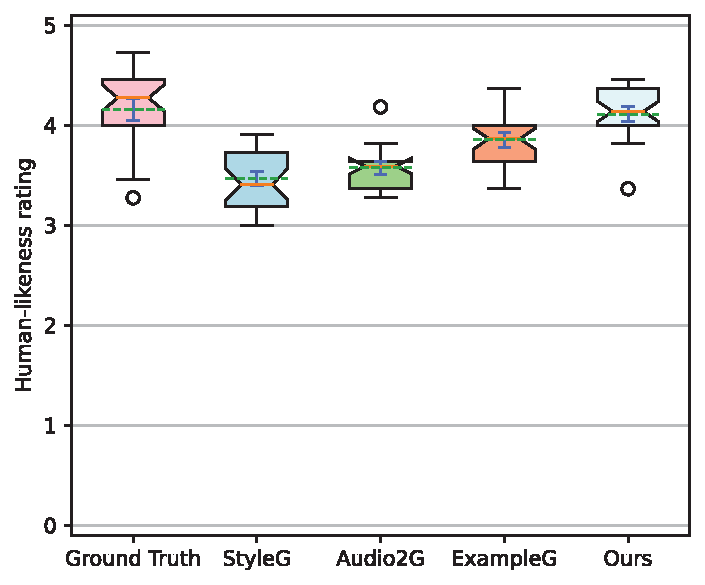
\includegraphics[width=\textwidth]{BoxHumanLikeness.pdf}
		\caption*{(a) Human-likeness}
	\end{subfigure}
	\hfill
	\begin{subfigure}[b]{0.3\textwidth}
		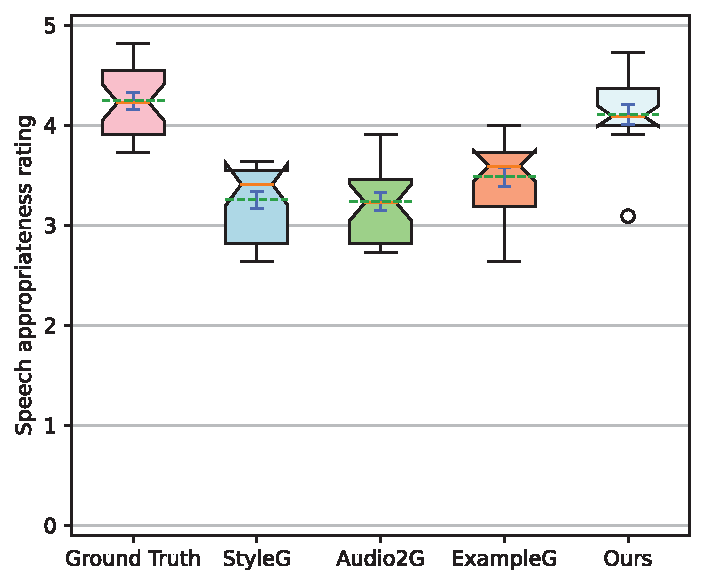
\includegraphics[width=\textwidth]{BoxSpeechAppropriateness.pdf}
		\caption*{\small (b) Speech Appropriateness}
	\end{subfigure}
	\hfill
	\begin{subfigure}[b]{0.3\textwidth}
		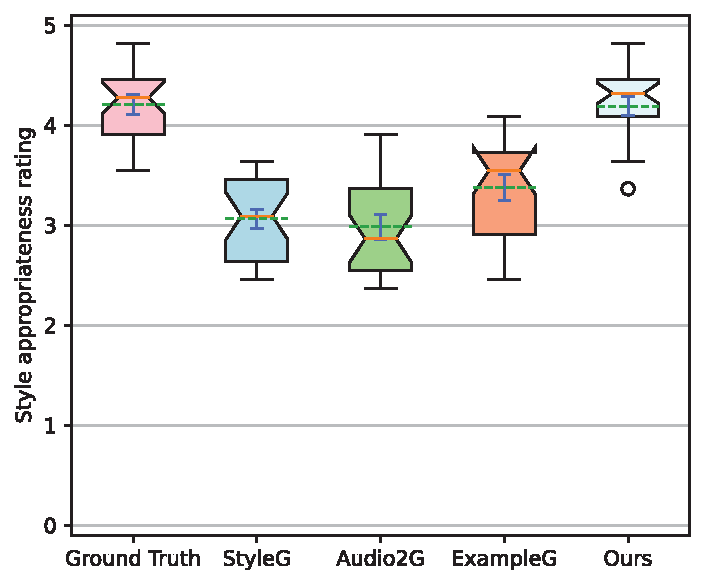
\includegraphics[width=\textwidth]{BoxStyleAppropriateness.pdf}
		\caption*{(c) Style Appropriateness}
	\end{subfigure}
	
	\label{fig:compare }
\end{figure}


Để hiểu hiệu suất thị giác thực tế của phương pháp của luận văn, luận văn tiến hành một nghiên cứu người dùng so sánh các cử chỉ được tạo ra từ phương pháp của luận văn và dữ liệu chụp chuyển động thực tế. Độ dài của các đoạn clip đánh giá dao động từ 11 đến 51 giây, với độ dài trung bình là 31.6 giây, dài hơn so với các đoạn trong đánh giá GENEA \cite{yoon2022genea} (8-10 giây), vì thời gian dài hơn có thể tạo ra kết quả rõ ràng và thuyết phục hơn \cite{yang2022reprgesture}. Người tham gia đánh giá trên thang điểm từ 5 đến 1, với các nhãn từ $\texttt{excellent}$,  $\texttt{good}$, $\texttt{fair}$, $\texttt{poor}$, đến $\texttt{bad}$. 

\begin{table}[H]
	\centering
	\begin{tabular}{lcc}
		\hline
		\multicolumn{1}{c}{Name} &
		\begin{tabular}[c]{@{}c@{}}Human\\ likeness \end{tabular}$\uparrow$ &
		\begin{tabular}[c]{@{}c@{}}Gesture-speech\\ appropriateness\end{tabular}$\uparrow$ \\ \hline
		Ground Truth          & 4.15 $\pm$ 0.11          & 4.25 $\pm$ 0.09          \\
		Ours                  & \textbf{4.11 $\pm$ 0.08} & \textbf{4.11 $\pm$ 0.10} \\
		\quad$-$ WavLM             & 4.05 $\pm$ 0.10          & 3.91 $\pm$ 0.11          \\
		\quad$-$ Cross-local attention   & 3.76 $\pm$ 0.09          & 3.51 $\pm$ 0.15          \\
		\quad$-$ Self-attention    & 3.55 $\pm$ 0.13          & 3.08 $\pm$ 0.10          \\
		\quad$-$ Attention + GRU&
		3.10 $\pm$ 0.11 &
		2.98 $\pm$ 0.14 \\
		\quad$+$ Forward attention & 3.75 $\pm$ 0.15          & 3.23 $\pm$ 0.24          \\
		\hline
	\end{tabular}
	\caption{Kết quả đánh giá bằng MOS}
	\label{table:MOSScore}
\end{table}
%Kết quả của các nghiên cứu loại bỏ (Ablation studies). "$-$" chỉ các mô-đun không được sử dụng và "$+$" chỉ các mô-đun bổ sung. Chữ in đậm chỉ ra chỉ số tốt nhất

\subsection{Kết quả đánh giá theo độ đo số học}

\subsubsection{Kết quả đánh giá bằng MSE}
\label{subsec:MSEResult}

Trong luận văn, chuỗi cử chỉ dự đoán sẽ được đoạn trên $M$ khung hình. Luận văn sử dụng Mean Square Error trên chuỗi cử chỉ $\mathbf{x}^{1:M \times D}$.

\begin{table}[H]
	\centering
	\resizebox{\textwidth}{!}{%
		\begin{tabular}{lcccccc}
			\hline
			\multicolumn{1}{c}{Cảm xúc} & Tự Nhiên & Buồn Bã &  Vui Vẻ  & Thư Giãn & Lớn Tuổi & Giận Dữ \\ \hline
			DiffuseStyleGesture  & 75.04 & 51.40 & 110.18 & 130.83     & 116.03    & 78.53     \\
			ZeroEGG & 136.33 & 81.22 & 290.47 & 140.24     & 102.44    & 181.07     \\
			\hline
			Mô hình đề xuất                     &         &         &         &           &          &                 \\
			\quad \textbf{OHGesture} & 161.22 & 89.58 & 279.95 & 156.93   & 99.86   & 215.24    \\
			\hline
		\end{tabular}%
	}
	\caption{Kết quả đánh giá Mean Square Error theo 6 cảm xúc}
	\label{table:EvaluationMSE}
\end{table}


\subsubsection{Kết quả đánh giá bằng FGD}

Luận văn đề xuất Fréchet Gesture Distance (FGD), độ đo FID dựa trên cử chỉ (gesture), và xây dựng mã nguồn \hyperlink{https://github.com/GestureScore/GestureScore}{GestureScore} \footnote{Github/GestureScore: \url{https://github.com/GestureScore/GestureScore}} . Trong GestureScore, luận văn xây dựng một Inception V3 model, để mã hóa chuỗi khung hình $\bx^{1:M \times D}$ thành vector tiềm ẩn kích thước $32 \times 32$. Sử dụng vector này làm đầu vào cho \autoref{eq:fidscore}. Sau đây là \autoref{table:EvalFGD} đánh giá kết quả của mô hình OHGesture bằng GestureScore

%$\uparrow$
\begin{table}[H]
	\centering
	\begin{tabular}{lcc}
		\hline
		\multicolumn{1}{c}{Name} & FGD trên vector đặc trưng & \begin{tabular}[c]{@{}c@{}} FGD dữ liệu gốc \end{tabular} \\ \hline
		Ground Truth             & -       & -          \\
		Ours                     &       & \\
		\quad OHGesture (Feature D=1141) & 2.058      & 9465.546 \\
		\quad OHGesture (Rotations) & 3.513       & 9519.129 \\
		\hline
	\end{tabular}
	\caption{Kết quả đánh giá Fréchet Gesture Distance (FGD) trên $\bx^{1:M \times D}$ (từ khung hình 1 đến khung hình M, mỗi khung hình có D đặc trưng từng khung hình )}
		\label{table:EvalFGD}
\end{table}

\begin{itemize}[]
		\item \textbf{Vector đặc trưng}
	Sử dụng tệp BVH để chuyển toàn bộ skeleton của mỗi khung hình thành vector đặc trưng $D = 1141 $ như công thức  \autoref{eq:gesturevector}
	
	\item  \textbf{Rotations}: Từ tệp BVH kết quả, luận văn trích xuất sự thay đổi của các góc quay (rotations), $D = 225$ ($225 = 75 \times 3$) của chuỗi cử chỉ với chiều dài mỗi đoạn là $M$ khung hình để đánh giá ở dòng OHGesture bên dưới. 
	
\end{itemize}

\section{Xây dựng và tiêu chuẩn hóa hệ thống đánh giá kết quả sinh cử chỉ}

Hiện nay các mô hình sinh (gesture generation) cử chỉ được quan tâm nghiên cứu với rất nhiều mô hình khác nhau, tuy nhiên do không có độ đo chung, vì các độ đo truyền thống như FID (Fréchet Inception Distance) hay IS (Inception Score),.. không thể hiện được hết các tính chất Giống người (Human-likeness), tính phù hợp với giọng nói (Speech Appropriateness), và tính phù hợp với phong cách (Style Appropriateness) của cử chỉ. Các mô hình cũng được thực hiện và huấn luyện trên một tập dữ liệu khác nhau, vì vậy rất khó để biết được mô hình nào đã đạt kết quả tốt hơn, và mô hình nào là mô hình state-of-the-art, từ đó khó có thể đạt được sự tiến bộ trong lĩnh vực sinh cử chỉ. Việc thiếu tiêu chuẩn chung để đánh giá trong cộng đồng nghiên cứu khiến luận văn mong muốn xây dựng một hệ thống xếp hạng trực tuyến \cite{nagy2024towards} \hyperlink{https://genea-workshop.github.io/leaderboard/}{GENEA Leaderboard} \footnote{GENEA Leaderboard: \url{https://genea-workshop.github.io/leaderboard/}}, là một bảng xếp hạng các mô hình sinh cử chỉ. Luận văn thu thập và xử lý một tập dữ liệu cử chỉ từ nhiều ngôn ngữ và từ nhiều tập dữ liệu khác nhau và tiêu chuẩn hóa để tạo ra một tập dữ liệu duy nhất.  Sau đó, luận văn sẽ mời các tác giả của các mô hình để học và dự đoán trên tập dữ liệu đã được tiêu chuẩn hóa, sau khi có kết quả sinh cử chỉ, luận văn sẽ thuê những người tham gia nghiên cứu trên Prolific để đánh giá và xếp hạng kết quả sinh cử chỉ của các mô hình. Hiện tại luận văn đang xây dựng hệ thống trực tuyến \hyperlink{https://github.com/hemvip/hemvip.github.io}{hemvip/hemvip.github.io}\footnote{HEMVIP2 \url{https://github.com/hemvip/hemvip.github.io}} với mục tiêu đánh giá kết quả sinh của cử chỉ thông qua việc thuê các người tham gia đánh giá kết quả thông qua Prolific. Luận văn sẽ bổ sung các đánh giá về mô hình OHGesture dựa trên các điểm số trên.


Thông qua hệ thống đánh giá này, nghiên cứu kỳ vọng sẽ thiết lập một tiêu chuẩn chung, từ đó tạo động lực cho sự tiến bộ trong lĩnh vực sinh cử chỉ.

%
%\chapter{CONCLUSION}
\label{Chapter5}

\section{Achieved Results}

This thesis has successfully developed and evaluated the gesture generation model OHGesture, a system capable of producing highly natural gestures that convey a human-like impression. A notable highlight of the model is its precise synchronization between gestures and the emotional content of the input speech, with the ability to generalize beyond the training data. This means the diffusion-based model is not solely dependent on the learned gesture data but also demonstrates strong generalization capabilities, enabling it to generate gestures for low-probability speech and contextual inputs.

Another significant aspect of this research is the expansion of input modalities. The thesis does not limit itself to gestures, speech, and emotion labels but also integrates text-to-speech tools to convert speech into text. By incorporating textual features, the model can better capture the semantic aspects of gestures, providing additional context and enabling the system to produce more appropriate and context-aware gestures.

\section{Strengths and Limitations of the Model}

The OHGesture model offers several significant advantages, contributing meaningfully to the development of more natural and flexible human-machine interaction systems. However, there remain some limitations that require future improvements for enhanced effectiveness.

\vspace{10pt}

\textbf{Strengths:}

\begin{itemize}
	\item \textbf{High realism:} Based on the gesture generation results, the OHGesture model produces gestures with a high degree of human-likeness. The generated gestures reflect the nuances and rhythm of speech, enabling the system to synchronize effectively with the emotional and semantic content of the speech.
	
	\item \textbf{Good generalization ability:} Thanks to the denoising model's capability to cover low-probability data points, the model can infer gestures for situations and emotional states not present in the training dataset, demonstrating potential for deployment in diverse real-world contexts.
	
	\item \textbf{Controllability over multiple attributes:} The diffusion model allows control over various emotional states and supports interpolation between different emotions.
\end{itemize}

\textbf{Limitations:}

\begin{itemize}
	\item The model currently lacks real-time inference capabilities and requires multiple steps to generate the final output.
	
	\item The feature representation with $D=1141$ is processed as an image, which does not fully capture motion characteristics.
	
	\item Dependence on high-quality input data: The model requires clear and high-quality speech input to ensure accurate gesture generation. When the input speech is noisy or contains ambiguous emotional variations, the accuracy of the generated gestures may degrade.
\end{itemize}

\section{Future Research and Development Directions}

Looking ahead, there are several promising directions to improve and expand the OHGesture gesture generation model to better meet practical requirements and enhance the system’s applicability. Key directions include:

\begin{itemize}
	\item \textbf{Optimizing the model for real-time inference:} Currently, the model requires speech sequences to be segmented, and the generated results must be imported into Unity for rendering. The thesis aims to develop real-time systems in the future to enable interactive applications and enhance the model's practicality.
	
	\item \textbf{Optimizing the sampling process and reducing sampling steps:} At present, the gesture generation process requires a relatively high number of sampling steps, which impacts the system’s speed and efficiency. Optimizing the process to reduce sampling steps without degrading gesture quality would enable faster responses suitable for real-time applications.
	
	\item \textbf{Integrating and experimenting with new embedding techniques:} Using novel embedding methods to diversify the input information may help the model better understand and reflect the context and emotions of speech. This development path would also enhance the system’s ability to generate semantically appropriate gestures across different languages.
	
	\item \textbf{Expanding to new languages:} Currently, the model primarily operates with English speech data. Extending the model to support gesture generation for various languages and cultures would be a significant advancement, making the system more diverse and widely applicable.
	
	\item \textbf{Combining with the DeepPhase model \cite{starke2022deepphase} to enable real-time gesture generation:} The thesis aims to integrate OHGesture with the DeepPhase model to develop systems capable of real-time gesture responses, suitable for natural interaction scenarios such as human-machine dialogue and voice-controlled systems. The goal is to learn phase-related motion features to extract motion characteristics more effectively, instead of treating features as image-like representations as done in the current model.
	
	\item \textbf{Improving objective evaluation with automatic metrics:} To reduce reliance on subjective evaluations, it is necessary to develop and incorporate reliable automatic evaluation methods, enabling the model to self-assess and adjust based on objective indicators.
\end{itemize}

\section{Thesis Contributions}
\label{sec:contribution}

In this thesis, the OHGesture gesture generation system was developed, with the following key contributions:

\begin{itemize}
	\item \textbf{Development of a gesture generation model based on Diffusion:} The OHGesture system is designed to generate gestures synchronized with input speech and accurately reflecting emotion. The model also possesses generalization capabilities, allowing gesture generation even for speech samples outside the training data, thereby achieving high realism.
	
	\item \textbf{Open-sourcing code and models on public platforms:} To encourage community adoption and improvement, the thesis provides source code on GitHub, with extensions and releases available at \hyperlink{https://github.com/hmthanh/OHGesture}{Github/OHGesture} \footnote{GitHub source code: \url{https://github.com/hmthanh/OHGesture}} and a pretrained version on Huggingface at \hyperlink{https://huggingface.co/openhuman/openhuman}{huggingface.co/openhuman/openhuman} \footnote{HuggingFace: \url{https://huggingface.co/openhuman/openhuman}}, enabling other researchers to easily access, reproduce, and extend the system.
	
	\item \textbf{Integration of text and transcribed speech in gesture generation:} Since the ZeroEGGS dataset includes only speech, gesture, and emotion labels, this thesis uses Azure and Google APIs to transcribe the speech files into text. This enriches the model’s input with textual features, giving the system additional context to produce more semantically appropriate gestures.
	
	\item \textbf{Contribution to standardized evaluation systems:} We developed an online ranking system \hyperlink{https://genea-workshop.github.io/leaderboard/}{GENEA Leaderboard} \footnote{GENEA Leaderboard: \url{https://genea-workshop.github.io/leaderboard/}} \cite{nagy2024towards} for gesture generation models. The GENEA Leaderboard collects and processes gesture data from multiple languages and datasets into a unified benchmark, allowing comparative evaluation across various models. Human evaluators are used to assess the models, providing more accurate evaluations of gesture generation results compared to previous metrics, which fail to capture the complexity and diversity of speech-related motion. This creates a unified data foundation that promotes consistent evaluation within the gesture generation research community.
	
	\item \textbf{Development of a Unity-based visualization tool:} Existing gesture visualization systems rely on Blender and do not render gestures effectively. By extending the source code of the DeepPhase model \cite{starke2022deepphase}, we developed a Unity-based rendering system \hyperlink{https://github.com/DeepGesture/deepgesture-unity}{Github/DeepGesture-Unity} \footnote{Unity-based gesture generation rendering system: \url{https://github.com/DeepGesture/deepgesture-unity}}.
	
	\item \textbf{Development of gesture evaluation using FGD (Fréchet Gesture Distance):} Based on the FGD source code \cite{yoon2020speech}, this thesis builds GestureScore and trains a new model to evaluate distribution differences in joint rotation angles between predicted and ground-truth data. The code is available at \hyperlink{https://github.com/GestureScore/GestureScore}{GestureScore} \footnote{Github/GestureScore: \url{https://github.com/GestureScore/GestureScore}} and the pretrained evaluation model is available on \hyperlink{https://huggingface.co/GestureScore}{Huggingface} \footnote{Huggingface/GestureScore: \url{https://huggingface.co/GestureScore/GestureScore}}.
	
	\item \textbf{Outlining future development directions:} Based on the diffusion model and a deep understanding of the gesture generation process, the thesis proposes integrating phase-based gesture generation models with advanced processing and feature extraction algorithms to optimize the quality and contextual alignment of generated gestures. This development direction opens up opportunities for significant improvements in gesture interaction with complex contextual elements such as facial expressions, prosody, and emotional dynamics, laying the groundwork for advancements in human-machine communication and related fields.
\end{itemize}

\newpage

\section{Closing Remarks}

Through experiments and analysis of gesture generation results, the OHGesture model developed in this thesis—an extension of the DiffuseStyleGesture model—demonstrates its ability to generate realistic gestures not only for data within the training set but also for out-of-distribution voices, such as that of Steve Jobs. This proves the potential of diffusion models for generating gestures in low-probability data contexts.

Furthermore, the thesis contributes modified source code on GitHub, including rendering and data processing pipelines based on Unity, providing a solid foundation for future research and improvements to the OHGesture model. The integration of textual input into the gesture generation process also represents a breakthrough, paving the way for applications in domains requiring more natural and effective human-computer interaction.

%
\pagebreak 
%TÀI LIỆU TRÍCH DẪN
\renewcommand{\bibname}{TÀI LIỆU THAM KHẢO} % Đổi tên phần tiêu đề của tài liệu tham khảo
%
\bibliographystyle{plain}
%\bibliographystyle{custombibstyle}
\bibliography{References/references}



%\renewcommand{\bibname}{DANH MỤC CÔNG TRÌNH CỦA HVCH}
%\bibliographystyle{plain}
%\bibliography{References/author}
%\printbibliography[heading=subbibliography,
%title={Web Related},
%keyword=web]
%\chapter*{TRÍCH NGANG THÔNG TIN BÀI BÁO KHOA HỌC LIÊN QUAN ĐẾN LUẬN VĂN THẠC SĨ	}
%\label{AppendixAuthor}
\chapter*{LIST OF THE MASTER’S PUBLISHED WORKS}
\label{AppendixAuthor}

\begin{enumerate}
	\item Towards a GENEA Leaderboard -- an Extended, Living Benchmark for Evaluating and Advancing Conversational Motion Synthesis \cite{nagy2024towards}.
%\item Tạp chí XYZ
\end{enumerate}

%\printbibliography[heading=subbibliography, title={Tiếng Việt}, keyword=Viet, resetnumbers=true]
%\bibliography{References/author.bib}

%\printbibliography[heading=subbibliography,
%title={Web Related},
%keyword=thanhminh]
%
%\appendix
\renewcommand{\chaptername}{Phụ lục}
\chapter{Các tham số trong Diffusion}
 \label{appendix:Appendix1}

\section{Sự thay đổi của $\sqrt{\alpha}$ và $\sqrt{1 - \alpha}$}

\begin{figure}[H]
	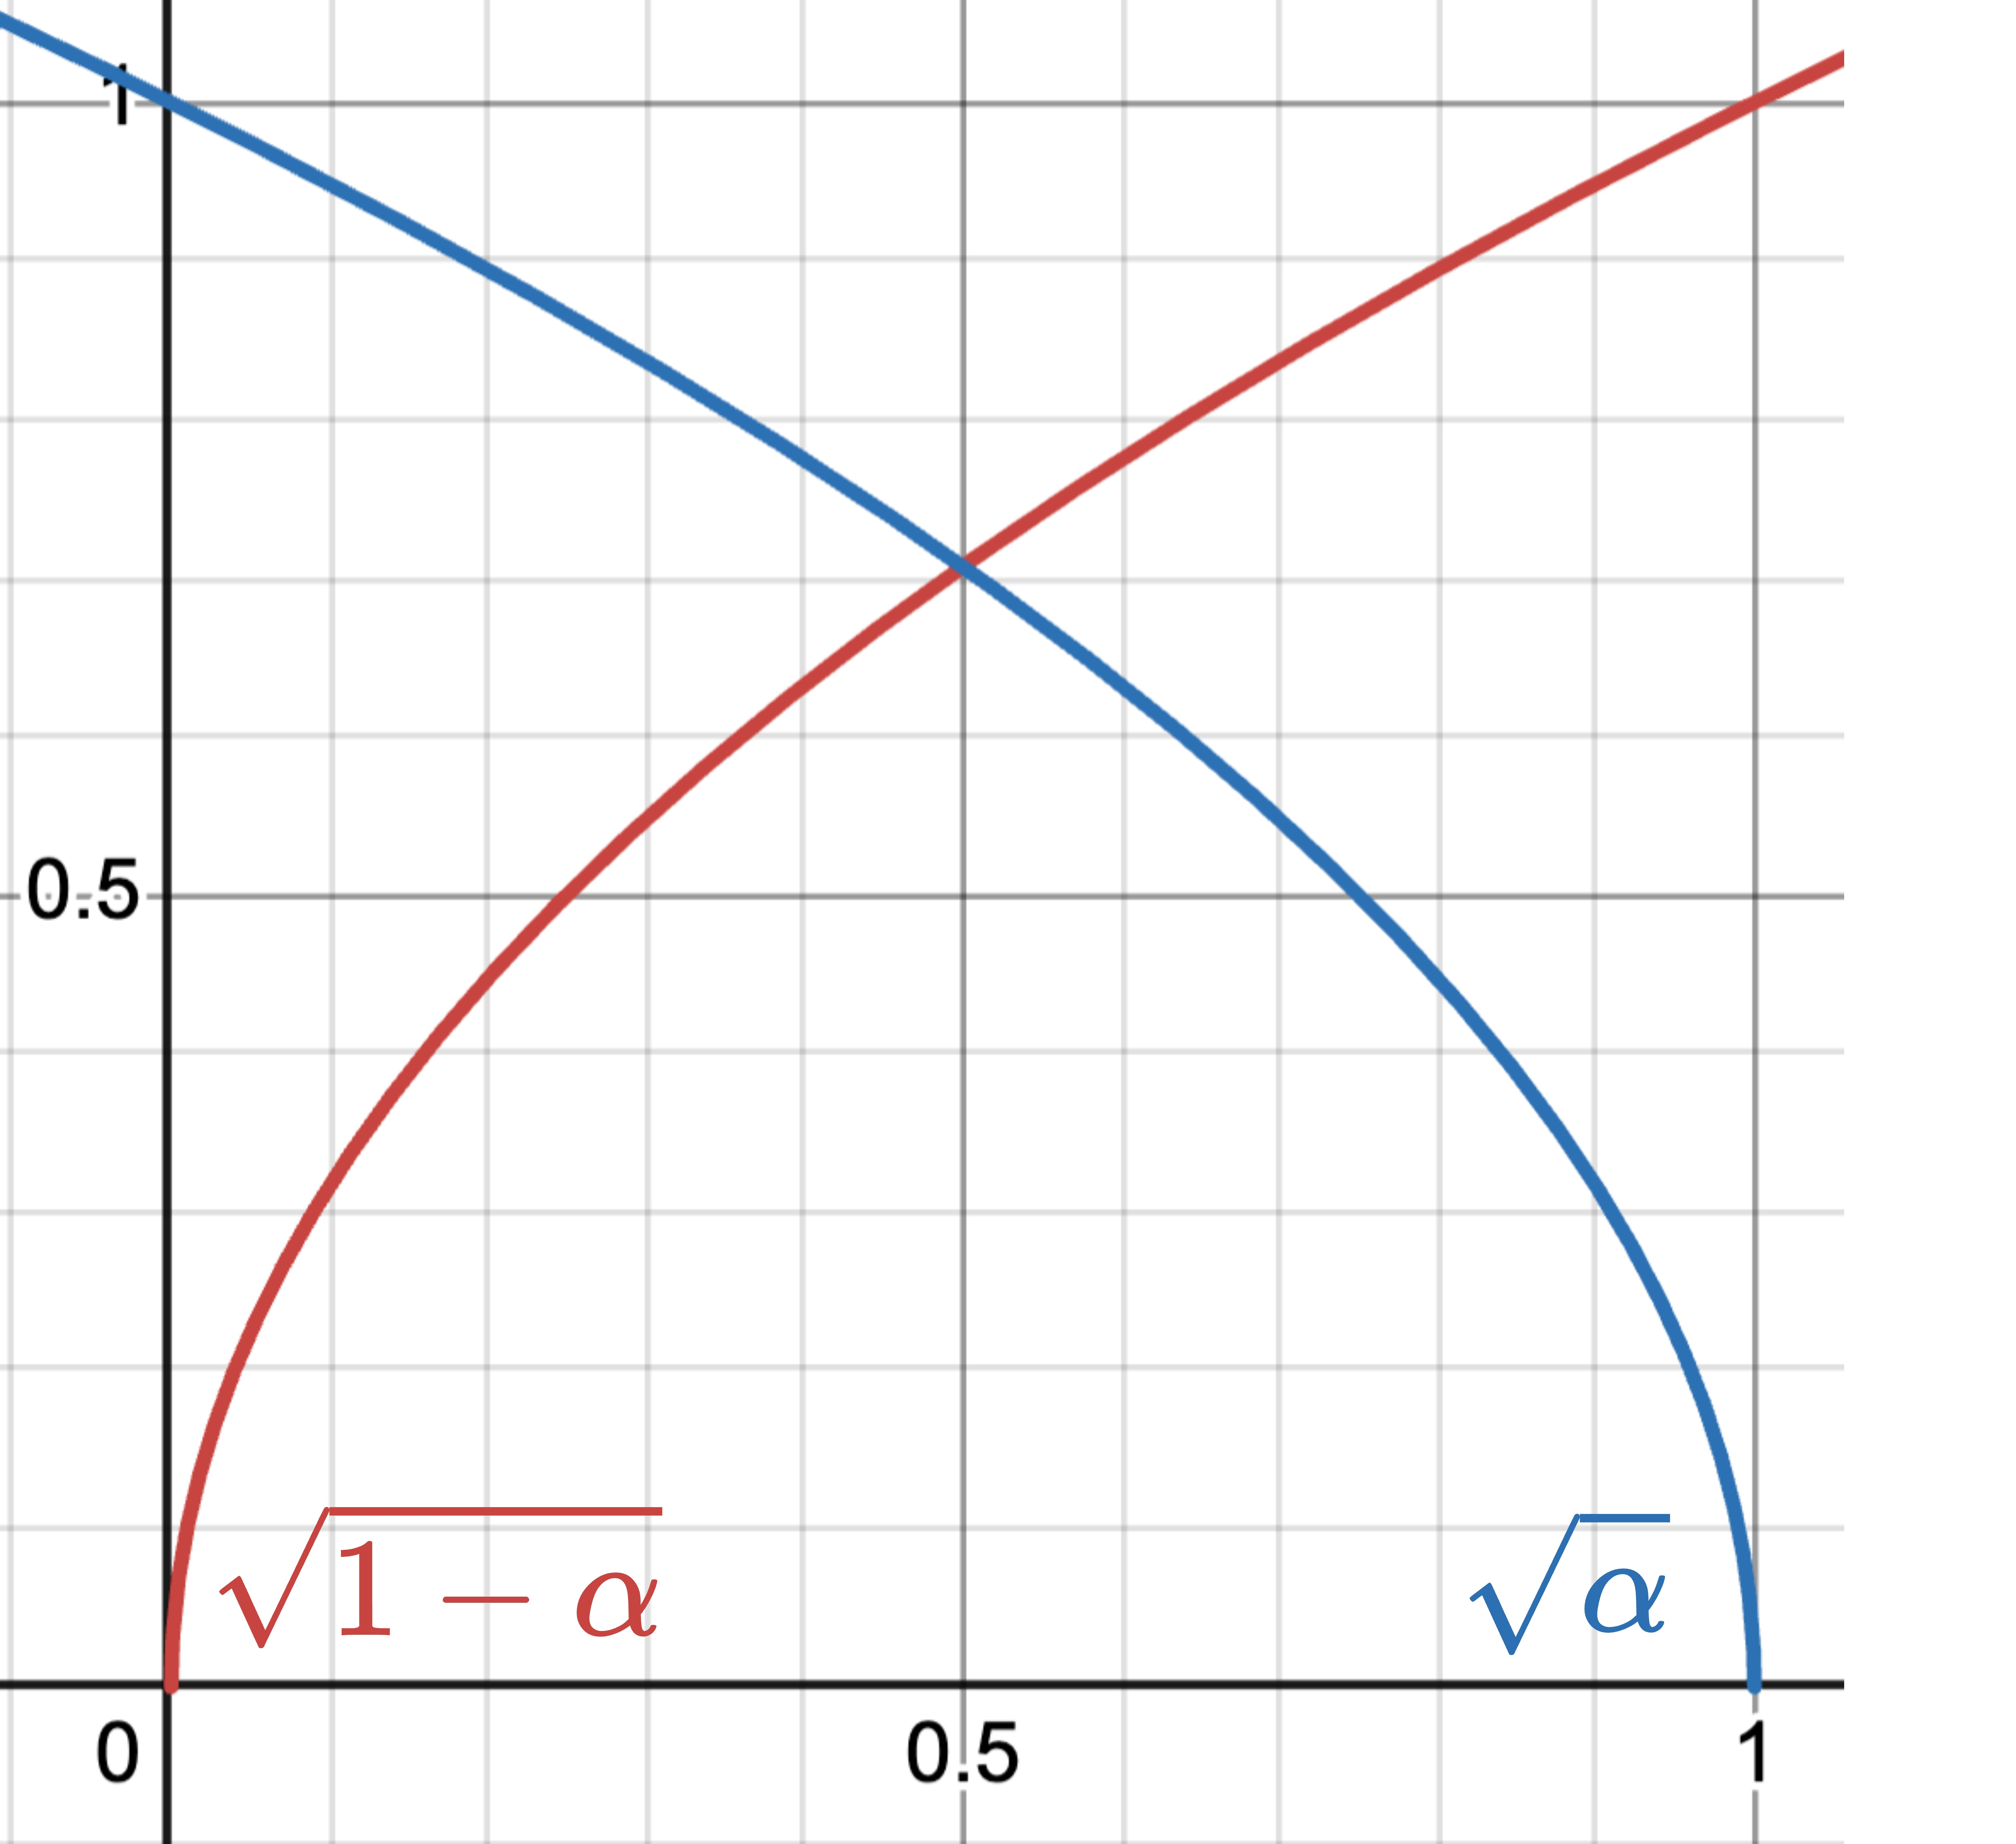
\includegraphics[width=0.5\linewidth]{SquareAlpha}
	\label{fig:wrapfig}
	\caption{Sự thay đổi của $\sqrt{\alpha}$ và $\sqrt{1 - \alpha}$}
\end{figure}

Trong quá trình diffusion, hệ thống muốn giảm dần sự hiện diện của $\bx$ và tăng dần sự hiện diện của nhiễu $\epsilon_t$. Với $\mathbf{x}_{t} = \sqrt{\alpha_t} \mathbf{x}_{t-1} + \sqrt{1 - \alpha_t} \epsilon_t$. Các hệ số $\sqrt{\alpha_t}$ và $\sqrt{1 - \alpha_t}$ giúp điều khiển quá trình này như sau:



\begin{itemize}
	\item $\sqrt{\alpha_t}$: Ban đầu giá trị lớn nhưng giảm dần để giảm sự ảnh hưởng vào kết quả tổng giữa nhiễu và $\bx_t$
	\item $\sqrt{1 - \alpha_t}$: Ban đầu giá trị nhỏ nhưng tăng dần theo từng bước. Với mục tiêu là đến cuối cùng thì sự ảnh hưởng của nhiễu càng lớn và trở thành nhiễu hoàn toàn.
\end{itemize}

Cả hai đại lượng này thay đổi theo thời gian trong quá trình diffusion, từ đó quyết định mức độ nhiễu được thêm vào từng bước $t$ và mức độ giữ lại trạng thái trước đó qua từng bước.


\section{Sự thay đổi của $\sqrt{\bar{\alpha}}$ và $\sqrt{1 - \bar{\alpha}}$}

$\bar{\alpha}_t = \prod_{i=1}^t \alpha_i$.  $\sqrt{1 - \bar{\alpha}_t} = \sqrt{1 - \prod_{i=1}^t \alpha_i}$. Cả $\sqrt{\bar{\alpha}}$ và $\sqrt{1 - \bar{\alpha}}$ đóng một vai trò quan trọng trong quá trình huấn luyện và sinh cử chỉ. Giúp kiểm soát mức độ nhiễu được thêm vào và cử chỉ, ta có thể thấy $\sqrt{\bar{\alpha}}$ giảm dần còn $\sqrt{1 - \bar{\alpha}}$ thì tăng dần..


\begin{figure}[H]
	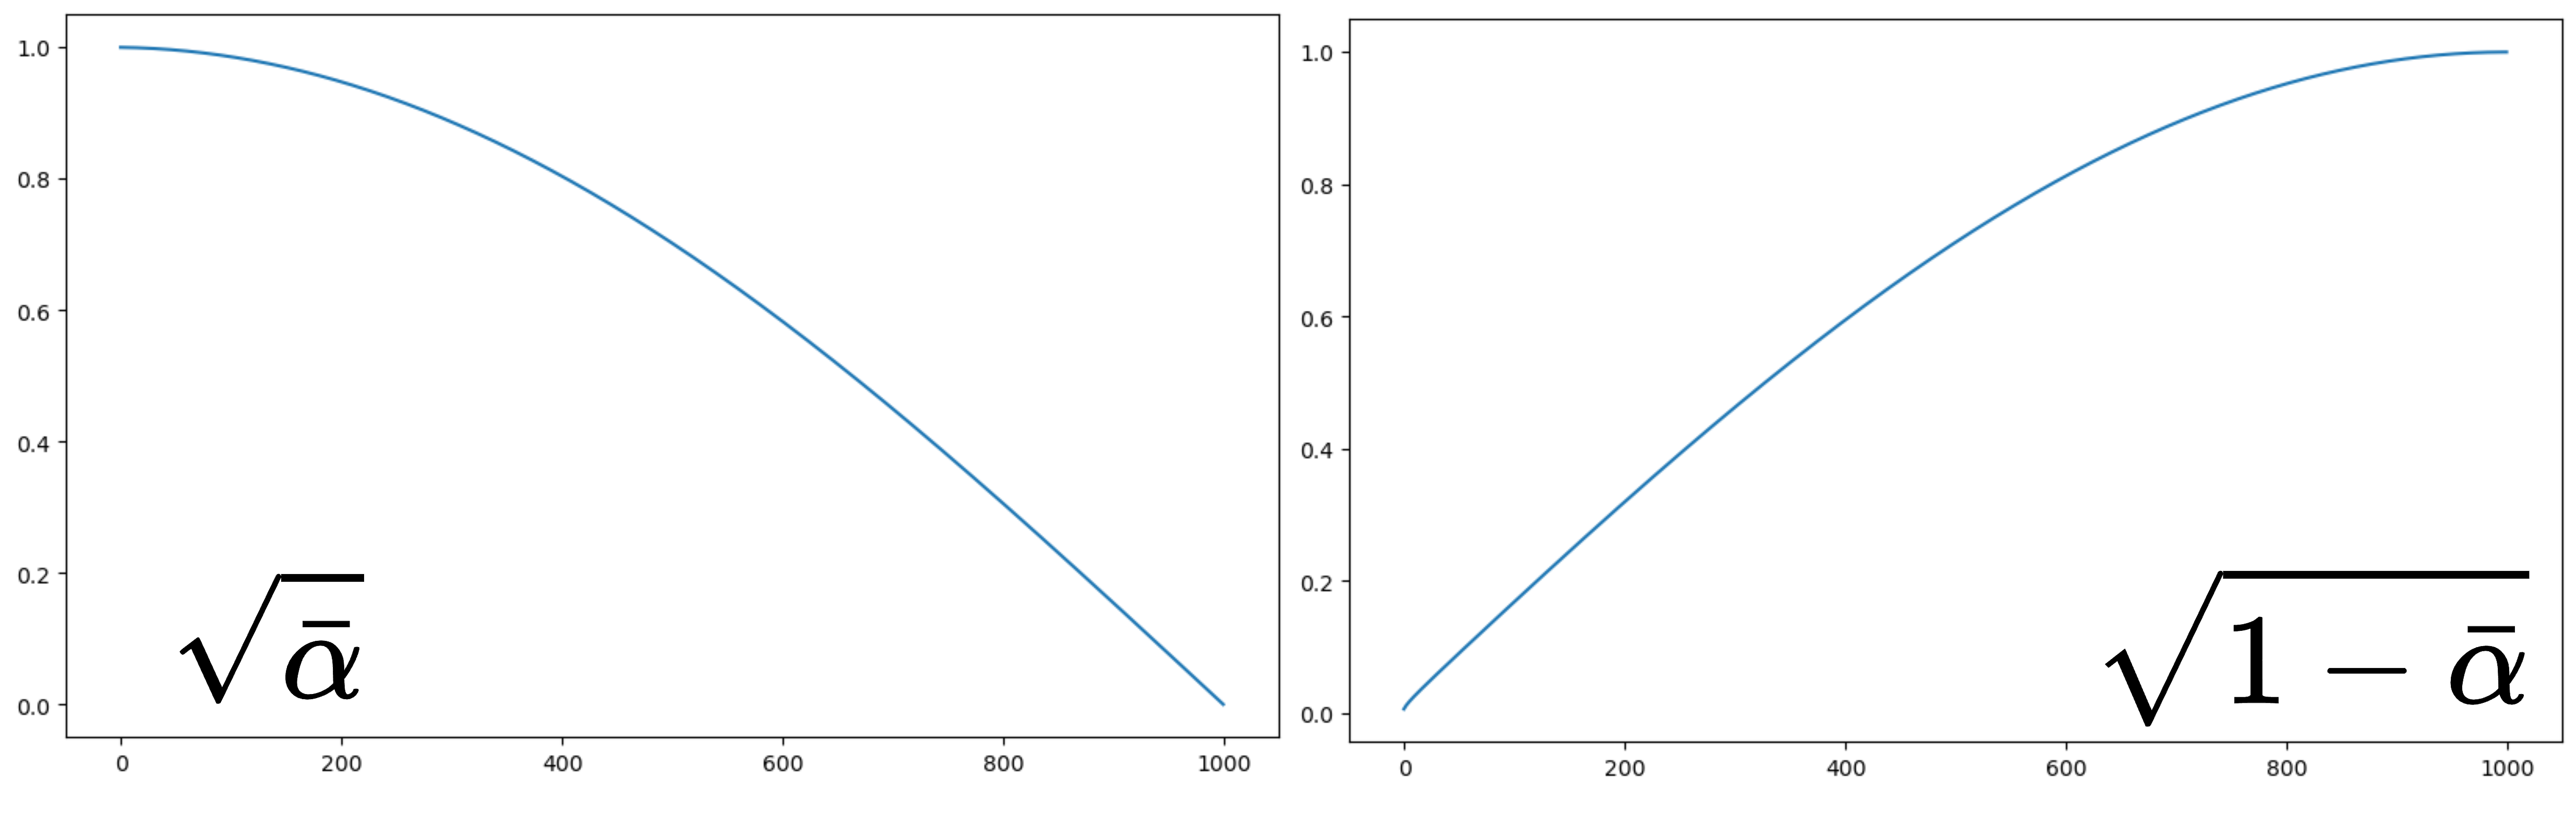
\includegraphics[width=\linewidth]{AlphaCumprod}
	\label{fig:AlphaCumprod}
	\caption{Quá trình thay đổi của $\sqrt{\bar{\alpha}}$ và $\sqrt{1 - \bar{\alpha}}$}
\end{figure}

%\section{So sánh $\epsilon$ objective và  $\bx_0$ }

\section{Sự thay đổi của $\sigma_t$}
 \label{appendix:Appendix1:NoiseScale}
\vspace{-10pt}
\begin{figure}[H]
	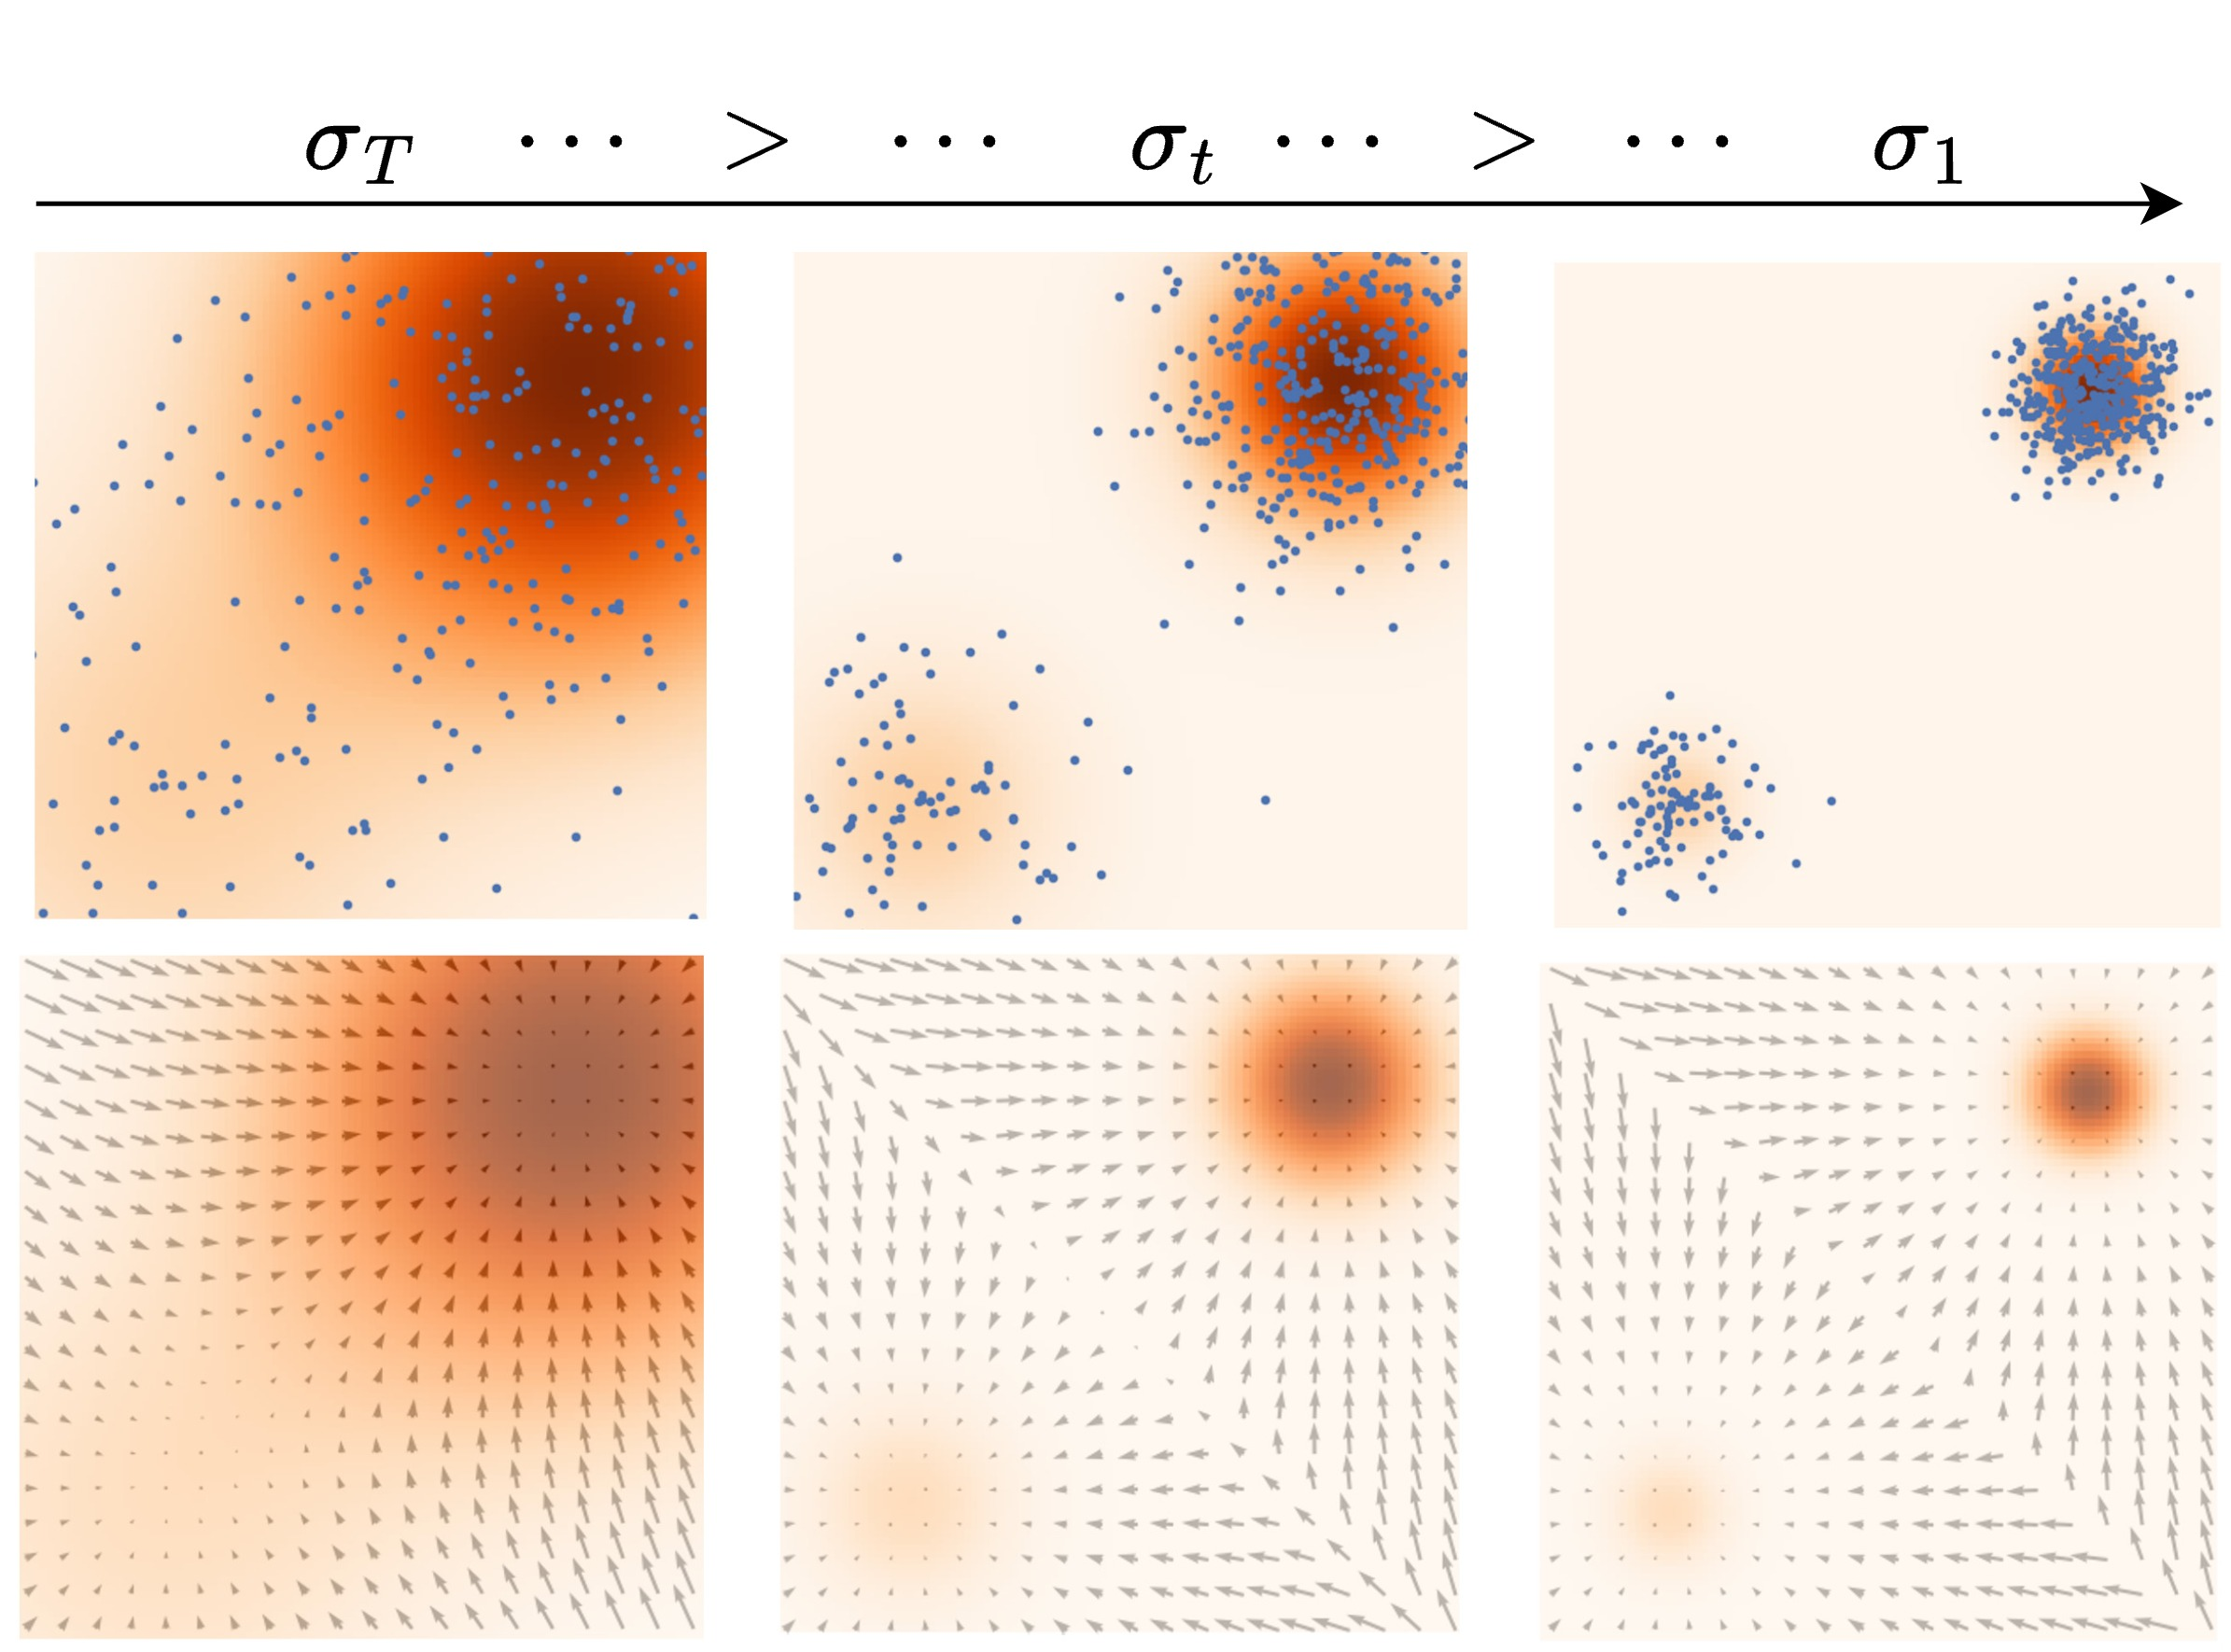
\includegraphics[width=\linewidth]{NoiseScale}
	\label{fig:NoiseScale}
	\caption{Sự thay đổi của hệ số $\sigma_t$ trong quá trình lấy mẫu }
\end{figure}
\vspace{-10pt}
Trong quá trình lấy mẫu, mục tiêu của việc giảm dần $\sigma_t$, mô hình có thể điều hướng về các vùng có mật độ dữ liệu cao ở từng bước $t$.


%\chapter{Quá trình xử lý dữ liệu BVH}
\label{appendix:BVHData}

\section{Cấu trúc khung xương của một nhân vật}
\label{appendix:BVHData:skeleton}

Một số tên khung xương nhân vật trong $75$ khung xương chuyển động bao gồm:

{
\small
\texttt{Hips},
\texttt{Spine},
\texttt{Neck},
\texttt{Head},
\texttt{RightShoulder},
\texttt{RightArm},
\texttt{RightForeArm},
\texttt{RightHand},
\texttt{LeftShoulder},
\texttt{LeftArm},
\texttt{LeftForeArm},
\texttt{LeftHand},
\texttt{RightUpLeg},
\texttt{RightLeg},
\texttt{RightFoot},
\texttt{RightToeBase},
\texttt{LeftUpLeg},
\texttt{LeftLeg},
\texttt{LeftFoot},
\texttt{LeftToeBase},
...
}

%\begin{itemize}
%	\item Left
%\end{itemize}

%\begincolcol}

\begin{figure}[H]
\centering
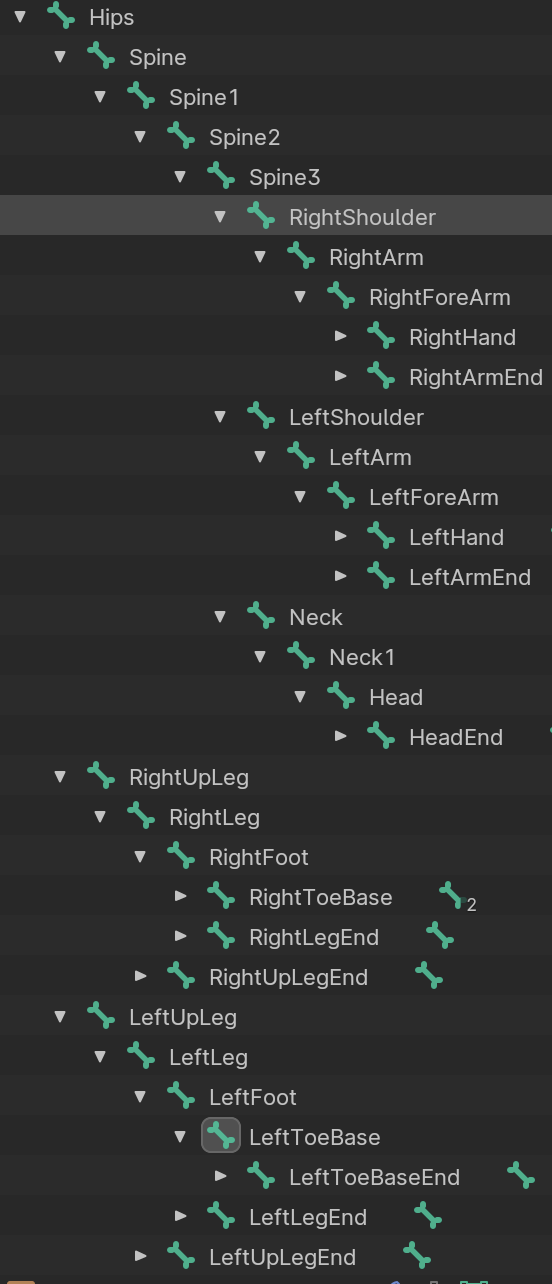
\includegraphics[height=10.5cm]{Bone}
\caption{Khung xương của một nhân vật}
\label{fig:Bone}
\end{figure}

\section{Cấu trúc tệp dữ liệu BVH}
\label{appendix:BVHData:BVHStructure}

File BVH (Biovision Hierarchy) là một định dạng file dữ liệu chứa thông tin về cấu trúc xương và dữ liệu về chuyển động của xương trong một hệ thống xương. File BVH bao gồm hai phần chính: phần khai báo cấu trúc xương và phần dữ liệu chuyển động của xương. 

\begin{itemize}
	\item \textbf{HIERARCHY}:
	
	\begin{itemize}
		\item Định nghĩa thành phần và tên các khung xương, vị trí khởi tạo của các khung xương ở vị trí T-pose (Tay diễn viên motion capture sẽ được duỗi thẳng thành hình chữ T).
		\item Định nghĩa quan hệ cha-con từ nút gốc đến các nút lá của một khung xương. Với nút gốc thường là cột sống ($\texttt{Spine}$).
		\item Định nghĩa các dữ liệu sẽ được ghi nhận như vị trí hoặc góc quay theo chiều $X, Y, Z$ của mỗi khung xương theo thời gian.
	\end{itemize}
	
	\item \textbf{MOTION}: Là chuỗi chuyển động theo từng khung hình, với mỗi khung hình là dữ liệu của từng xương về chuyển động theo thông tin về góc quay hoặc vị trí đã định nghĩa ở HIERARCHY.
\end{itemize}

\begin{figure}[htbp]
	\centering
	\begin{subfigure}{0.49\textwidth}
		\centering
		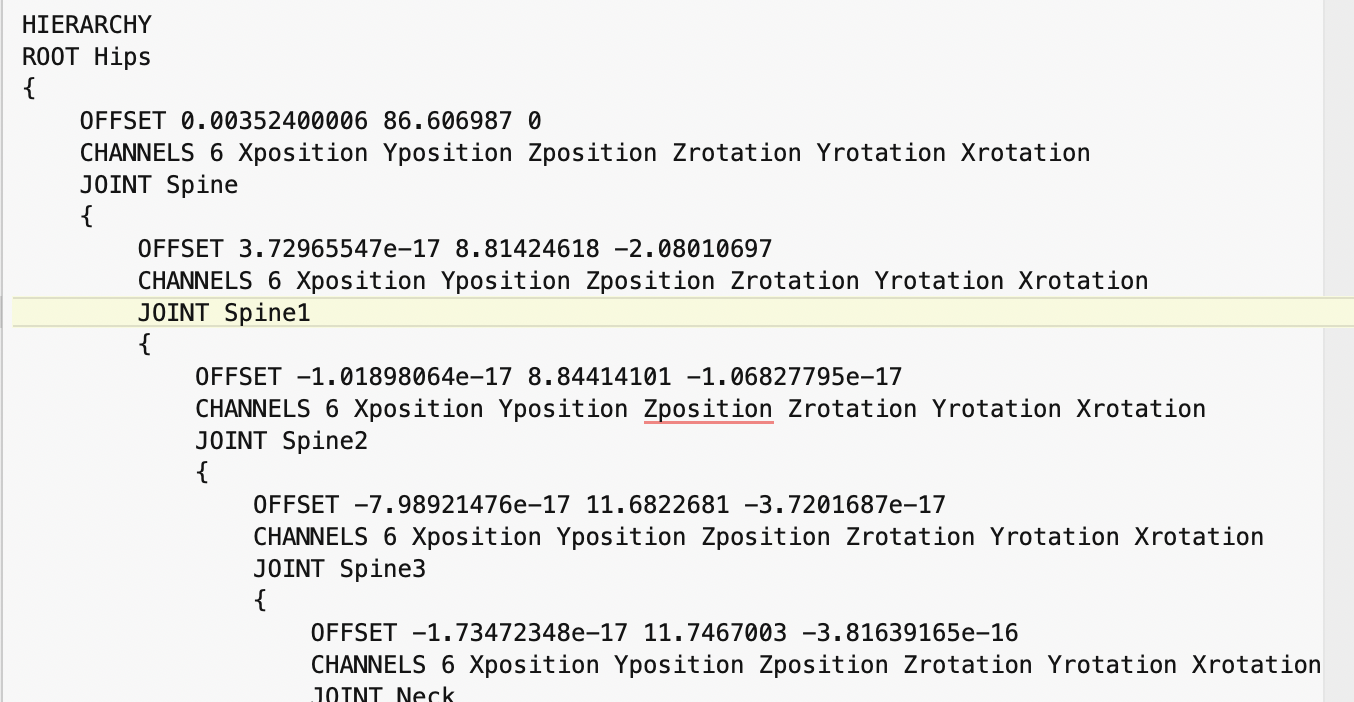
\includegraphics[width=\linewidth]{BVH1}
		\caption{HIERARCHY trong tệp BVH}
		\label{fig:BVH1}
	\end{subfigure}
	\hfill
	\begin{subfigure}{0.49\textwidth}
		\centering
		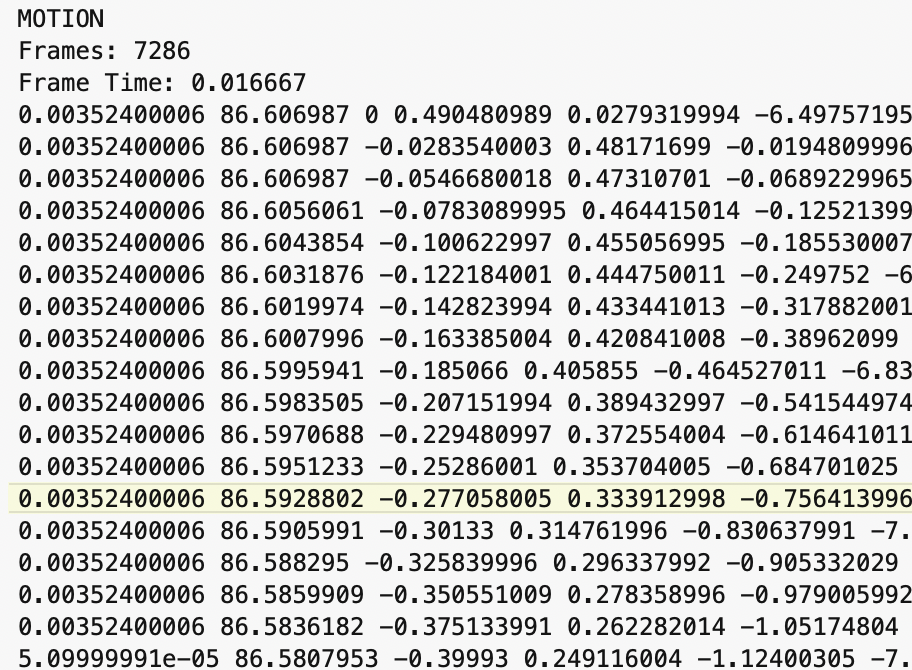
\includegraphics[width=\linewidth]{BVH2}
		\caption{MOTION trong tệp BVH}
		\label{fig:BVH2}
	\end{subfigure}
\end{figure}




%	\begin{figure}
	%		\centering
	%		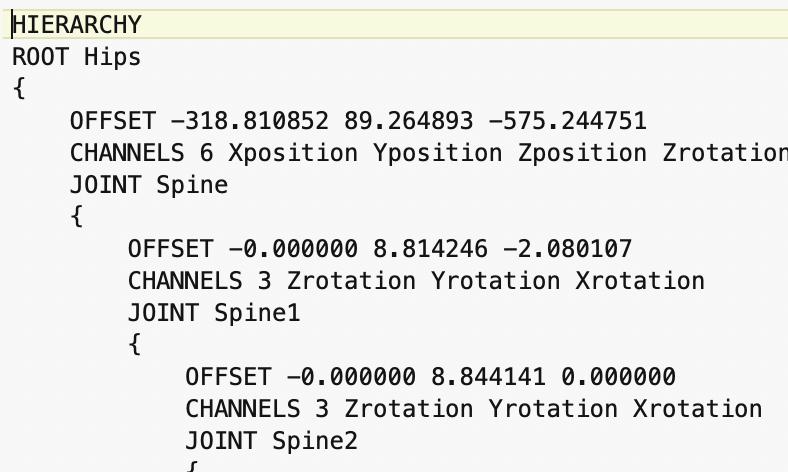
\includegraphics[width=0.25\textwidth]{BVHFile}
	%	\end{figure}
	
$\mathbf{rotation}_i^{\operatorname{local}} = \{ \alpha ,\beta , \gamma \}$ lần lượt là góc quay quanh các trục $Z$ ,$Y$ , và $X$, góc quay tổng hợp ba trục trong không gian Euler là 

\begin{equation}
R = R_Z(\alpha) R_Y(\beta) R_X(\gamma)
\end{equation}

Trong đó:

1. \textbf{Ma trận quay quanh trục \(Z\)}:

\[
R_Z(\alpha) = 
\begin{bmatrix}
	\cos(\alpha) & -\sin(\alpha) & 0 \\
	\sin(\alpha) & \cos(\alpha) & 0 \\
	0 & 0 & 1
\end{bmatrix}
\]

2. \textbf{Ma trận quay quanh trục \(Y\)}:

\[
R_Y(\beta) = 
\begin{bmatrix}
	\cos(\beta) & 0 & \sin(\beta) \\
	0 & 1 & 0 \\
	-\sin(\beta) & 0 & \cos(\beta)
\end{bmatrix}
\]

3. \textbf{Ma trận quay quanh trục \(X\)}:

\[
R_X(\gamma) = 
\begin{bmatrix}
	1 & 0 & 0 \\
	0 & \cos(\gamma) & -\sin(\gamma) \\
	0 & \sin(\gamma) & \cos(\gamma)
\end{bmatrix}
\]

Để tính tọa độ chuyển động của một nhân vật, thực hiện phép toán sau:

\begin{equation}
	\mathbf{position}_{\text{global}} = R \cdot \mathbf{position}_{\text{local}} + \mathbf{t}
\end{equation}


\section{Quá trình chuyển góc quay Euler sang Quaternion}
\label{appendix:BVHData:QuaternionConvert}


Để tránh Gimbal lock, dữ liệu ở dạng góc quay Euler phải được chuyển sang dạng góc quay Quaternion. Trong đó góc quay từng Bone dạng Euler ZYX sang dạng Quaternion, mỗi Bone biểu diễn bằng 4 phần tử $q = (q_w, q_x, q_y, q_z)$, với các giá trị được tính như sau:
%	Mỗi Bone được biểu diễn thành: 

Đầu tiên, tính các giá trị $\cos$ và $\sin$ của một nửa góc quay cho mỗi trục:


\begin{itemize}
	\item $c_{\alpha} = \cos\left(\frac{\alpha}{2}\right), \quad s_{\alpha} = \sin\left(\frac{\alpha}{2}\right)$
	\item $c_{\beta} = \cos\left(\frac{\beta}{2}\right), \quad s_{\beta} = \sin\left(\frac{\beta}{2}\right)$
	\item $c_{\gamma} = \cos\left(\frac{\gamma}{2}\right), \quad s_{\gamma} = \sin\left(\frac{\gamma}{2}\right)$
\end{itemize}

Dựa trên các giá trị tính được ở trên, các thành phần của quaternion được tính như sau:


\begin{itemize}
	\item $q_w = c_{\alpha} c_{\beta} c_{\gamma} + s_{\alpha} s_{\beta} s_{\gamma}$
	\item $q_x = c_{\alpha} c_{\beta} s_{\gamma} - s_{\alpha} s_{\beta} c_{\gamma}$
	\item $q_y = c_{\alpha} s_{\beta} c_{\gamma} + s_{\alpha} c_{\beta} s_{\gamma}$
	\item $q_z = s_{\alpha} c_{\beta} c_{\gamma} - c_{\alpha} s_{\beta} s_{\gamma}$
\end{itemize}

Với quaternion $q$ đã tính, vị trí toàn cục của bone $\mathbf{p}_{\text{global}}$ được xác định bằng cách quay vị trí cục bộ $\mathbf{p}_{\text{local}}$ thông qua công thức:

\begin{equation}
	\mathbf{p}_{\text{global}} = q \cdot \mathbf{p}_{\text{local}} \cdot q^{-1} + \mathbf{t}
\end{equation}

với $\mathbf{t}$ là vị trí gốc của bone trong không gian toàn cục.
%\input{Appendix/Appendix3}

\end{document}